\documentclass[paper=a4wide, fontsize=11pt]{report}	 % A4 paper and 11pt font size
\usepackage[svgnames]{xcolor} % Using colors
\usepackage{xurl} %xurl en vez de url para urls largas
\usepackage[hidelinks]{hyperref}
\usepackage[utf8]{inputenc}
\renewcommand\thechapter{\Roman{chapter}}
\usepackage[spanish]{babel} % ponerlo en español
\usepackage{todonotes} % para poner notitas de colores
\usepackage{fancyhdr} % Needed to define custom headers/footers
\usepackage[a4paper, left=30mm, right=30mm, top=2.5cm, bottom=2.5cm, footskip=1.2cm]{geometry}  % Changing size of document
\usepackage{braket}
\usepackage{tabularx}
\usepackage{multirow}
\usepackage{nicematrix}
\usepackage[numbers]{natbib}
\usepackage{subcaption}
\usepackage{tabularx, makecell, booktabs}
\usepackage{textcmds}
\usepackage{color}
\usepackage{listings}
\definecolor{lightgray}{rgb}{.9,.9,.9}
\definecolor{darkgray}{rgb}{.4,.4,.4}
\definecolor{purple}{rgb}{0.65, 0.12, 0.82}
%%%%%% Setting up the style

\pagestyle{fancy} % Enables the custom headers/footers

\lhead{} \rhead{} % Headers - all  empty



\title{
{\Huge \textbf{Proyecto: 
\\ Sistemas de Información 2}}\\
\vspace{1cm}
\vspace{1cm}
\text{Pablo Angusto\quad\href{mailto:842255@unizar.es}{842255@unizar.es}}\\
\text{Miguel Aréjula\quad\href{mailto:850068@unizar.es}{850068@unizar.es}}\\

\includegraphics[width=6cm]{logo.png}\\
\date{6 de marzo de 2024}



}


\cfoot{\color{Black} \thepage}

\renewcommand{\headrulewidth}{0.0pt} % No header rule
\renewcommand{\footrulewidth}{0.4pt} % Thin footer rule
\renewcommand{\thesection}{\arabic{section}} % para que los títulos no salgan en 0.1 ...

\setcounter{secnumdepth}{3}
%%%%%% Starting the document
\setlength\parindent{0pt} % No indentar los párrafos
\begin{document}
\author{Pablo Angusto and Miguel Aréjula}
\maketitle % Print the title
\tableofcontents
\newpage
\thispagestyle{fancy} % Enabling the custom headers/footers for the first page

% In the following lines, add the relevant information
\vspace{-0.5cm}

%TODO add content
\section{Introducción}

Odoo es un software de código abierto para la gestión empresarial. Destaca por ser una plataforma versátil con diversas áreas funcionales de una organización. Con un enfoque modular, Odoo ofrece una gran cantidad de aplicaciones; contabilidad, recursos humanos, ventas, inventario, CRM y más, permitiendo a las empresas optimizar sus procesos y centralizar su gestión.


Esta software modular facilita a las empresas la adaptación a sus necesidades específicas. La interfaz intuitiva y la naturaleza de código abierto de Odoo fomentan la personalización y la innovación continua, brindando a las empresas la flexibilidad necesaria para evolucionar con el cambiante panorama empresarial. Odoo está posicionada como una herramienta valiosa para impulsar el crecimiento y la eficacia operativa de las organizaciones.

\section{Instalación}
\paragraph{}
UZ-On-Marketing esta buscando introducir un ERP en su empresa. Algunas de las posiblidades son SAP, SAGE u Odoo. La empresa no dispone de mucho presupuesto para invertir en el ERP, por lo tanto, se ha decido utilizar la versión 17 de Odoo al ser de código abierto y tener coste cero.

\paragraph{}
Para instalar Odoo en las máquinas de la empresa hay varias opciones: instalar en paquetes, instalación en linea, instalación de origen o mediante Docker.
Hemos decidido instalarlo mediante docker ya que es una manera sencilla y rápida de obtener Odoo. 
Para ello es necesario tener instalado docker en nuestra máquina. En caso que no lo tengamos, podemos obtenerlo de diversas formas en función del  sistema operativo que tenga la máquina: 
\subsection{Instalación Docker}
\begin{itemize}
    \item \textbf{Windows:} 
    \begin{enumerate}
        \item Descarga Docker Desktop desde el sitio oficial de Docker: Docker Desktop for Windows.
        \item Ejecuta el instalador descargado y sigue las instrucciones del asistente de instalación.
        \item Durante la instalación, se te pedirá que habilites la virtualización en la BIOS de tu computadora, si aún no está habilitada. Asegúrate de seguir estas instrucciones si es necesario.
        \item Una vez completada la instalación, reinicia tu ordenador si es necesario.
    \end{enumerate}
    \item \textbf{MacOS: }
    \begin{enumerate}
        \item Descarga Docker Desktop desde el sitio oficial de Docker: Docker Desktop for Mac.
        \item Ejecuta el instalador descargado y arrastra el ícono de Docker a la carpeta de Aplicaciones.
        \item Abre Docker Desktop desde la carpeta de Aplicaciones.
    \end{enumerate}
    \item \textbf{Linux:} 
    \begin{itemize}
        \item \textbf{Sistemas basados en Debian (ej:Ubuntu)}
        \begin{enumerate}
            \item Actualiza el índice de paquetes: 
            \begin{lstlisting}[frame=single, basicstyle=\small]
sudo apt update
            \end{lstlisting}
            \item Instala paquetes para permitir que APT use un repositorio sobre HTTPS:
            \begin{lstlisting}[frame=single, basicstyle=\small]
sudo apt install apt-transport-https ca-certificates curl
software-properties-common
            \end{lstlisting}
            
            \item Agrega la clave GPG para el repositorio oficial de Docker:
            \begin{lstlisting}[frame=single, basicstyle=\small]
curl -fsSL https://download.docker.com/linux/ubuntu/gpg | sudo 
gpg --dearmor -o /usr/share/keyrings/docker-archive-keyring.gpg
            \end{lstlisting}
            
            \item Agrega el repositorio de Docker al sistema:
            \begin{lstlisting}[frame=single, basicstyle=\tiny]
echo "deb [signed-by=/usr/share/keyrings/docker-archive-keyring.gpg]
https://download.docker.com/linux/ubuntu \$(lsb\_release -cs) stable"
| sudo tee /etc/apt/sources.list.d/docker.list > /dev/null
            \end{lstlisting}
            
            \item Actualiza el índice de paquetes nuevamente:
           \begin{lstlisting}[frame=single, basicstyle=\small]
sudo apt update
            \end{lstlisting}
            \item Instala Docker:
            \begin{lstlisting}[frame=single, basicstyle=\small]
sudo apt install docker-ce docker-ce-cli containerd.io
            \end{lstlisting}
        \end{enumerate}
        \item \textbf{Sistemas basados en Red Hat (ej:Fedora)}
        \begin{enumerate}
            \item Instala Docker utilizando el gestor de paquetes dnf:
            \begin{lstlisting}[frame=single, basicstyle=\small]
sudo dnf install docker
            \end{lstlisting}
            \item Inicia y habilita el servicio Docker:
            \begin{lstlisting}[frame=single, basicstyle=\small]
sudo systemctl start docker
sudo systemctl enable docker
            \end{lstlisting}
        \end{enumerate}
        Para verificar que se ha instalado correctamente Docker ejecuta el comando:
        \begin{lstlisting}[frame=single, basicstyle=\small]
docker --version
        \end{lstlisting}
             Finalmente, para poder utilizar docker se va a necesitar los permisos de administrador por lo que puedes usar sudo o añadir tu usuario al grupo "docker" mediante el comando:
              \begin{lstlisting}[frame=single, basicstyle=\small]
sudo usermod -aG docker user.
        \end{lstlisting}
    \end{itemize}
\end{itemize}
\subsection{Instalación Odoo}
\paragraph{}
Una vez instalado docker, se va a continuar con la instalación de Odoo. El siguiente paso es crear un fichero con el nombre docker-compose.yml
\begin{lstlisting}[frame=single, basicstyle=\small]
version: "3.1"
services:
  odoo:
    image: odoo:17.0
    depends_on:
      - db
    ports:
      - "8069:8069"
    volumes:
      - odoo-web-data:/var/lib/odoo
    environment:
      - HOST=db
      - USER=odoo
      - PASSWORD=myodoo
  db:
    image: postgres:13
    environment:
      - POSTGRES_DB=postgres
      - POSTGRES_PASSWORD=myodoo
      - POSTGRES_USER=odoo
      - PGDATA=/var/lib/postgresql/data/pgdata
    volumes:
      - odoo-db-data:/var/lib/postgresql/data/pgdata
volumes:
  odoo-web-data:
  odoo-db-data:
\end{lstlisting}
\paragraph{}
A continuación, se necesita abrir una terminal y dirigerte al directorio donde se localiza el fichero docker-compose.yml. Para arrancar Odoo ejecuta en la terminal el comando docker compose up –d. Además, si se quiere parar Odoo se deberá ejecutar el comando docker compose stop o eliminarlo con docker compose down. Tras arrancar Odoo, para acceder a él se debe ir al navegador instalado en la máquina y escribir en la barra de busqueda de la parte superior la dirección http://localhost:8069/.
Redirige a /web/database/selector??? e introducir la siguiente información en el formulario, pulsar en create database y esperar a que se cree la base de datos.
\begin{figure}[h]
    \centering
    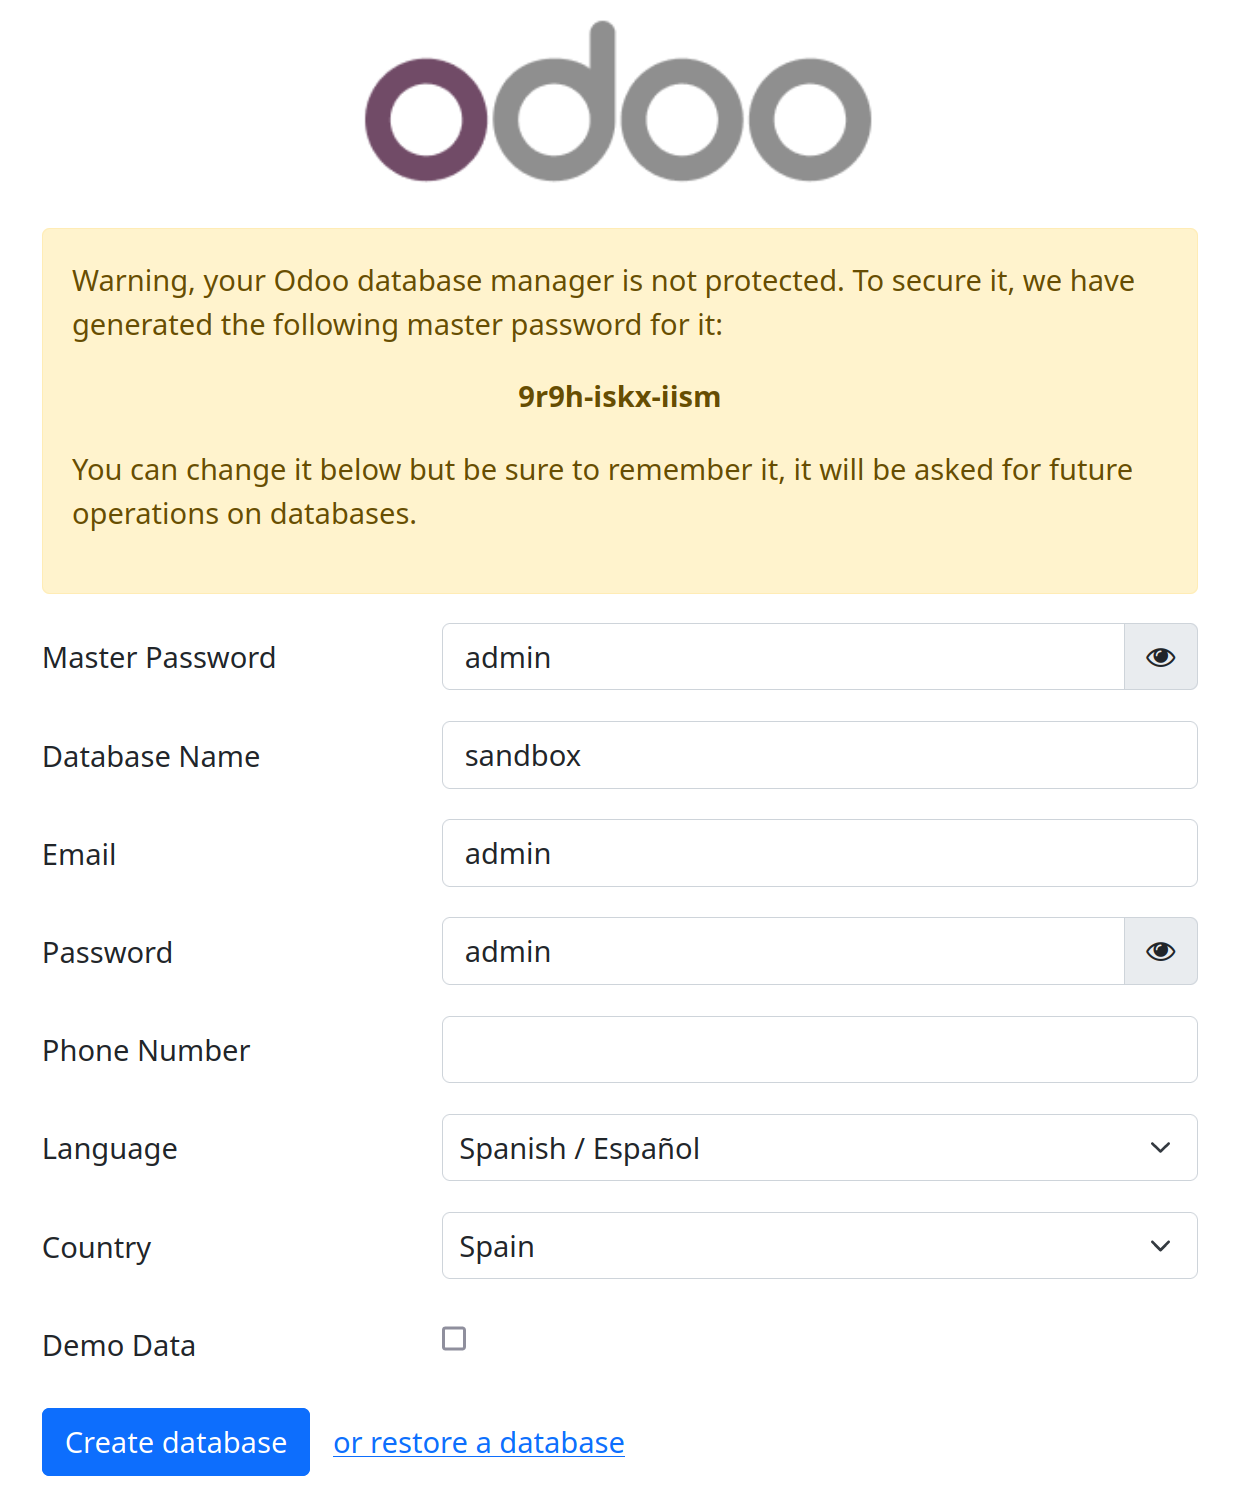
\includegraphics[width=6cm]{signup.png}
    \caption{Proceso de registro en Odoo}
    \label{fig:signup}
\end{figure}
Por último, cuando se tenga que iniciar sesión se tendrá que introducir el usuario admin y la contraseña admin.
\paragraph{}
Una vez dentro de Odoo, elimina el filtro de Aplicaciones de la barra de búsqueda y busca Blog.
\begin{figure}[h]
    \centering
    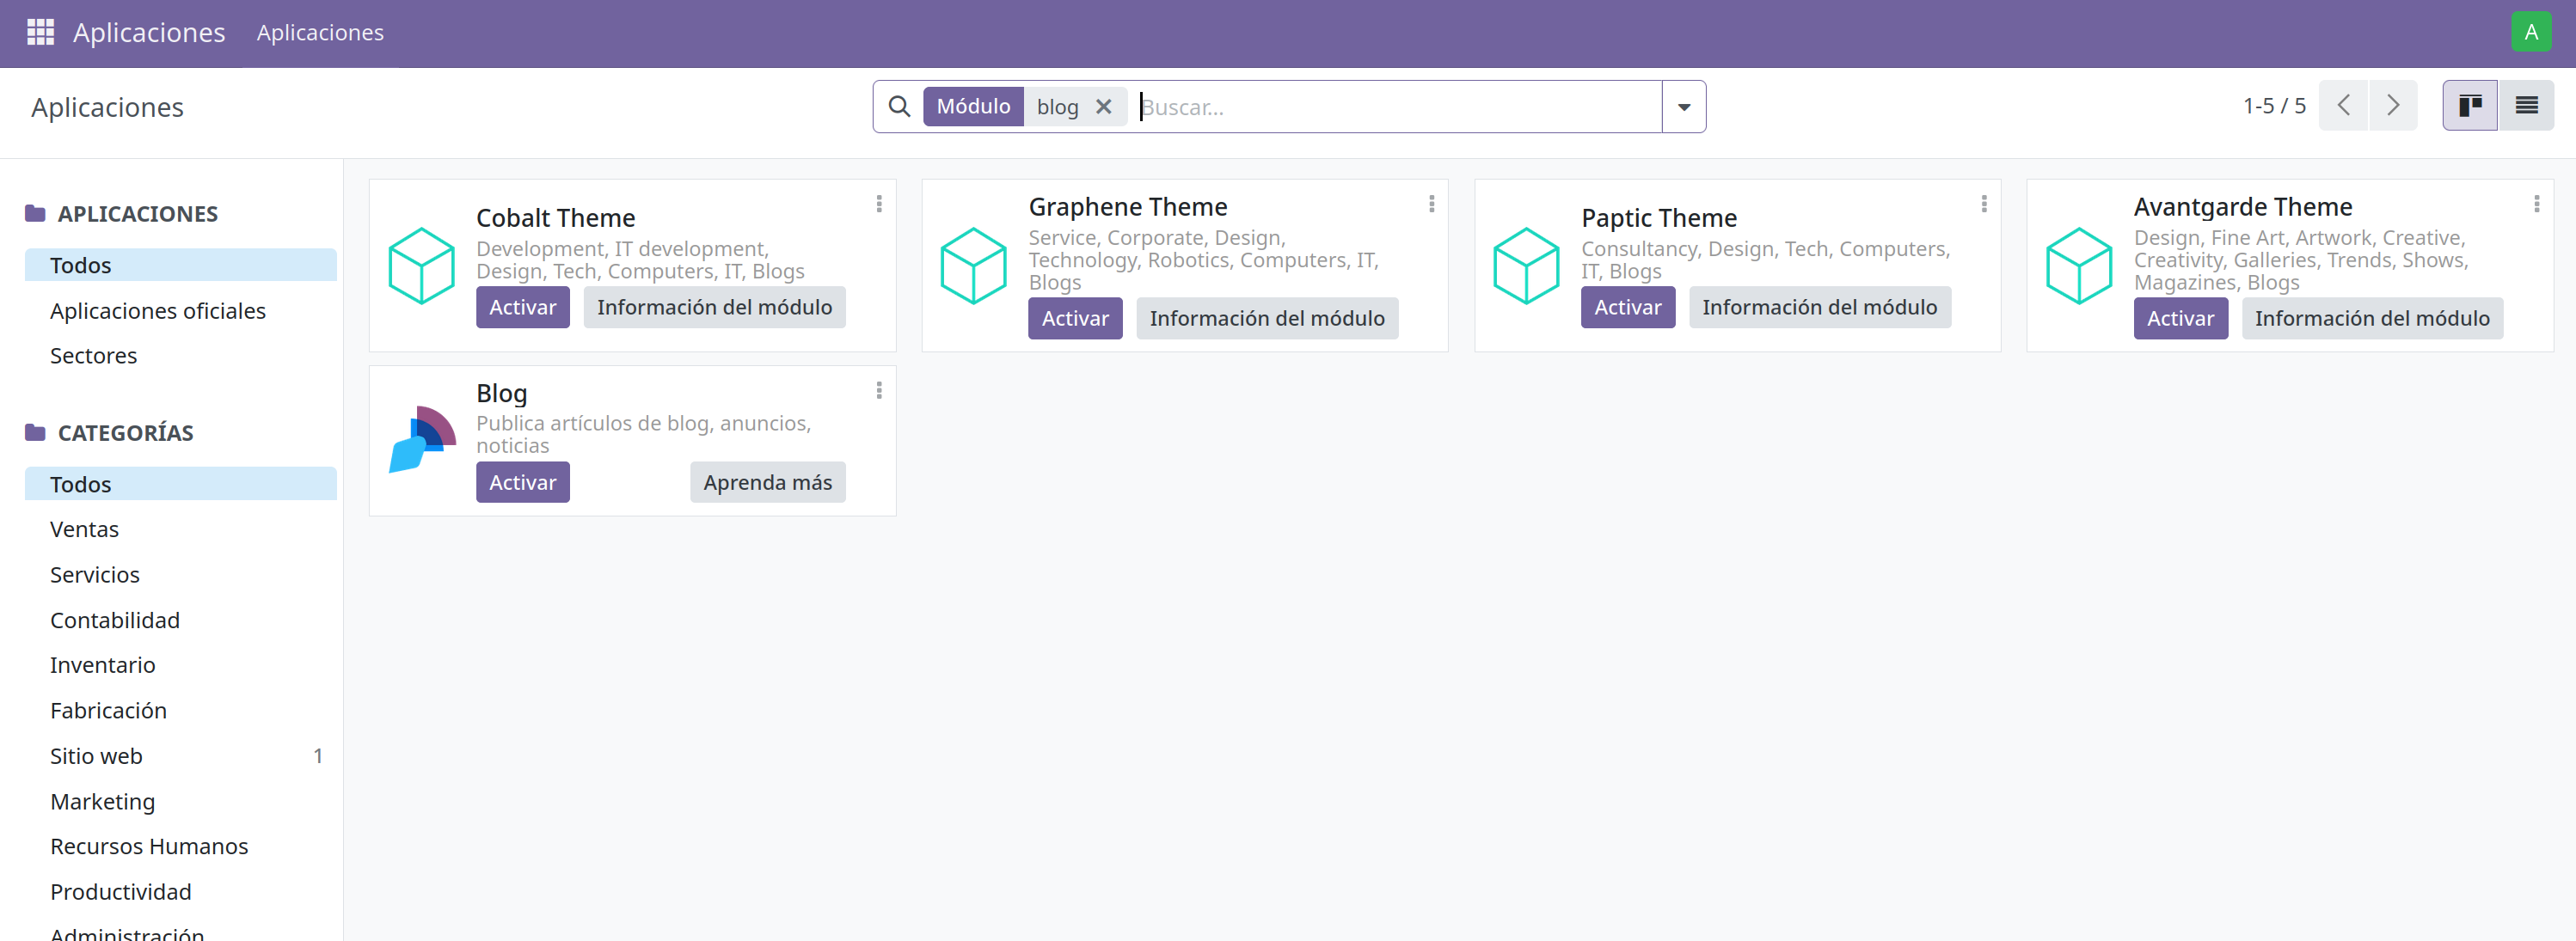
\includegraphics[width=6cm]{blog.png}
    \caption{Busqueda y activación del Blog}
    \label{fig:blog}
\end{figure}
\paragraph{}
Haz click en Activar dentro de la tarjeta de Blog, de esta manera se instalará automáticamente los módulos relacionados con la web. Se mostrará la siguiente pantalla:
\begin{figure}[h]
    \centering
    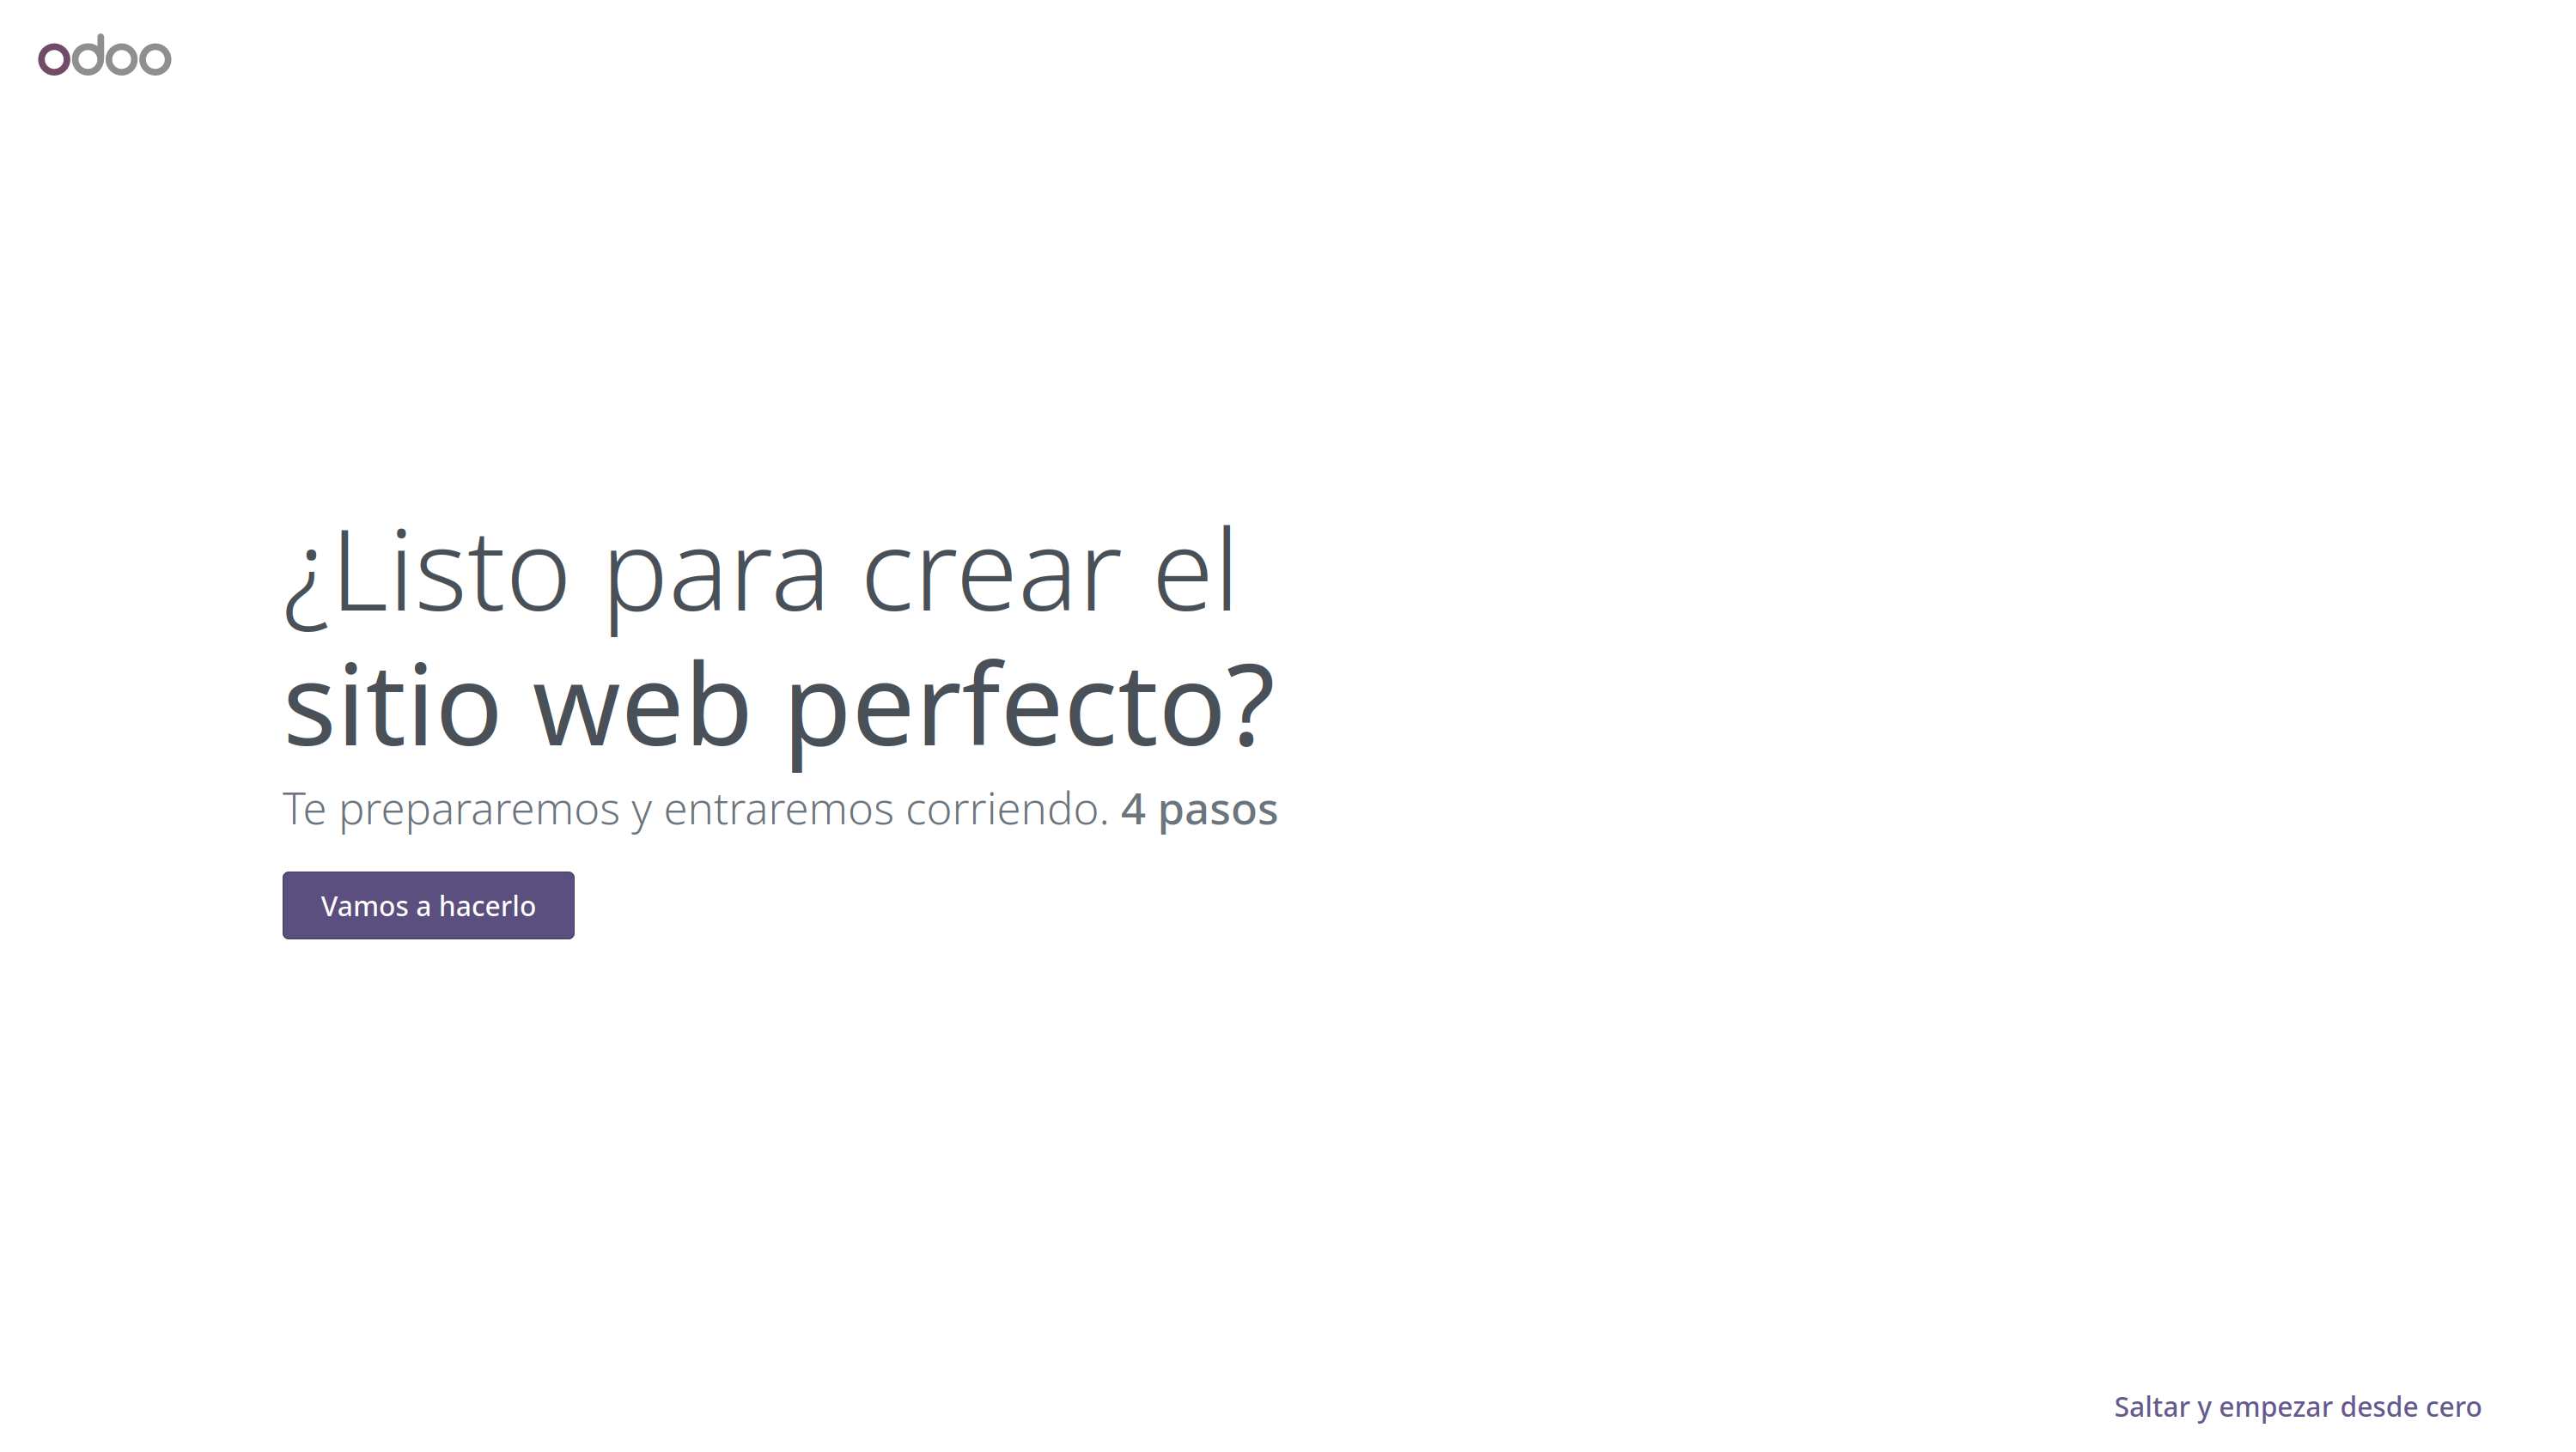
\includegraphics[width=6cm]{tutorial.png}
    \caption{Creación de la web}
    \label{fig:tutorial}
\end{figure}
En este menú se seleccionará la opción de Vamos a hacerlo, que permitirá crear la web de forma sencilla en 4 pasos. Selecciona e introduce la información que más se adecua al caso en particular y personaliza los colores y las características que tendrá la web. A continuación, se creará la web siguiendo la información enviada y se mostrará, en este caso se ha creado una web de alquiler de coches:
\begin{figure}[h]
    \centering
    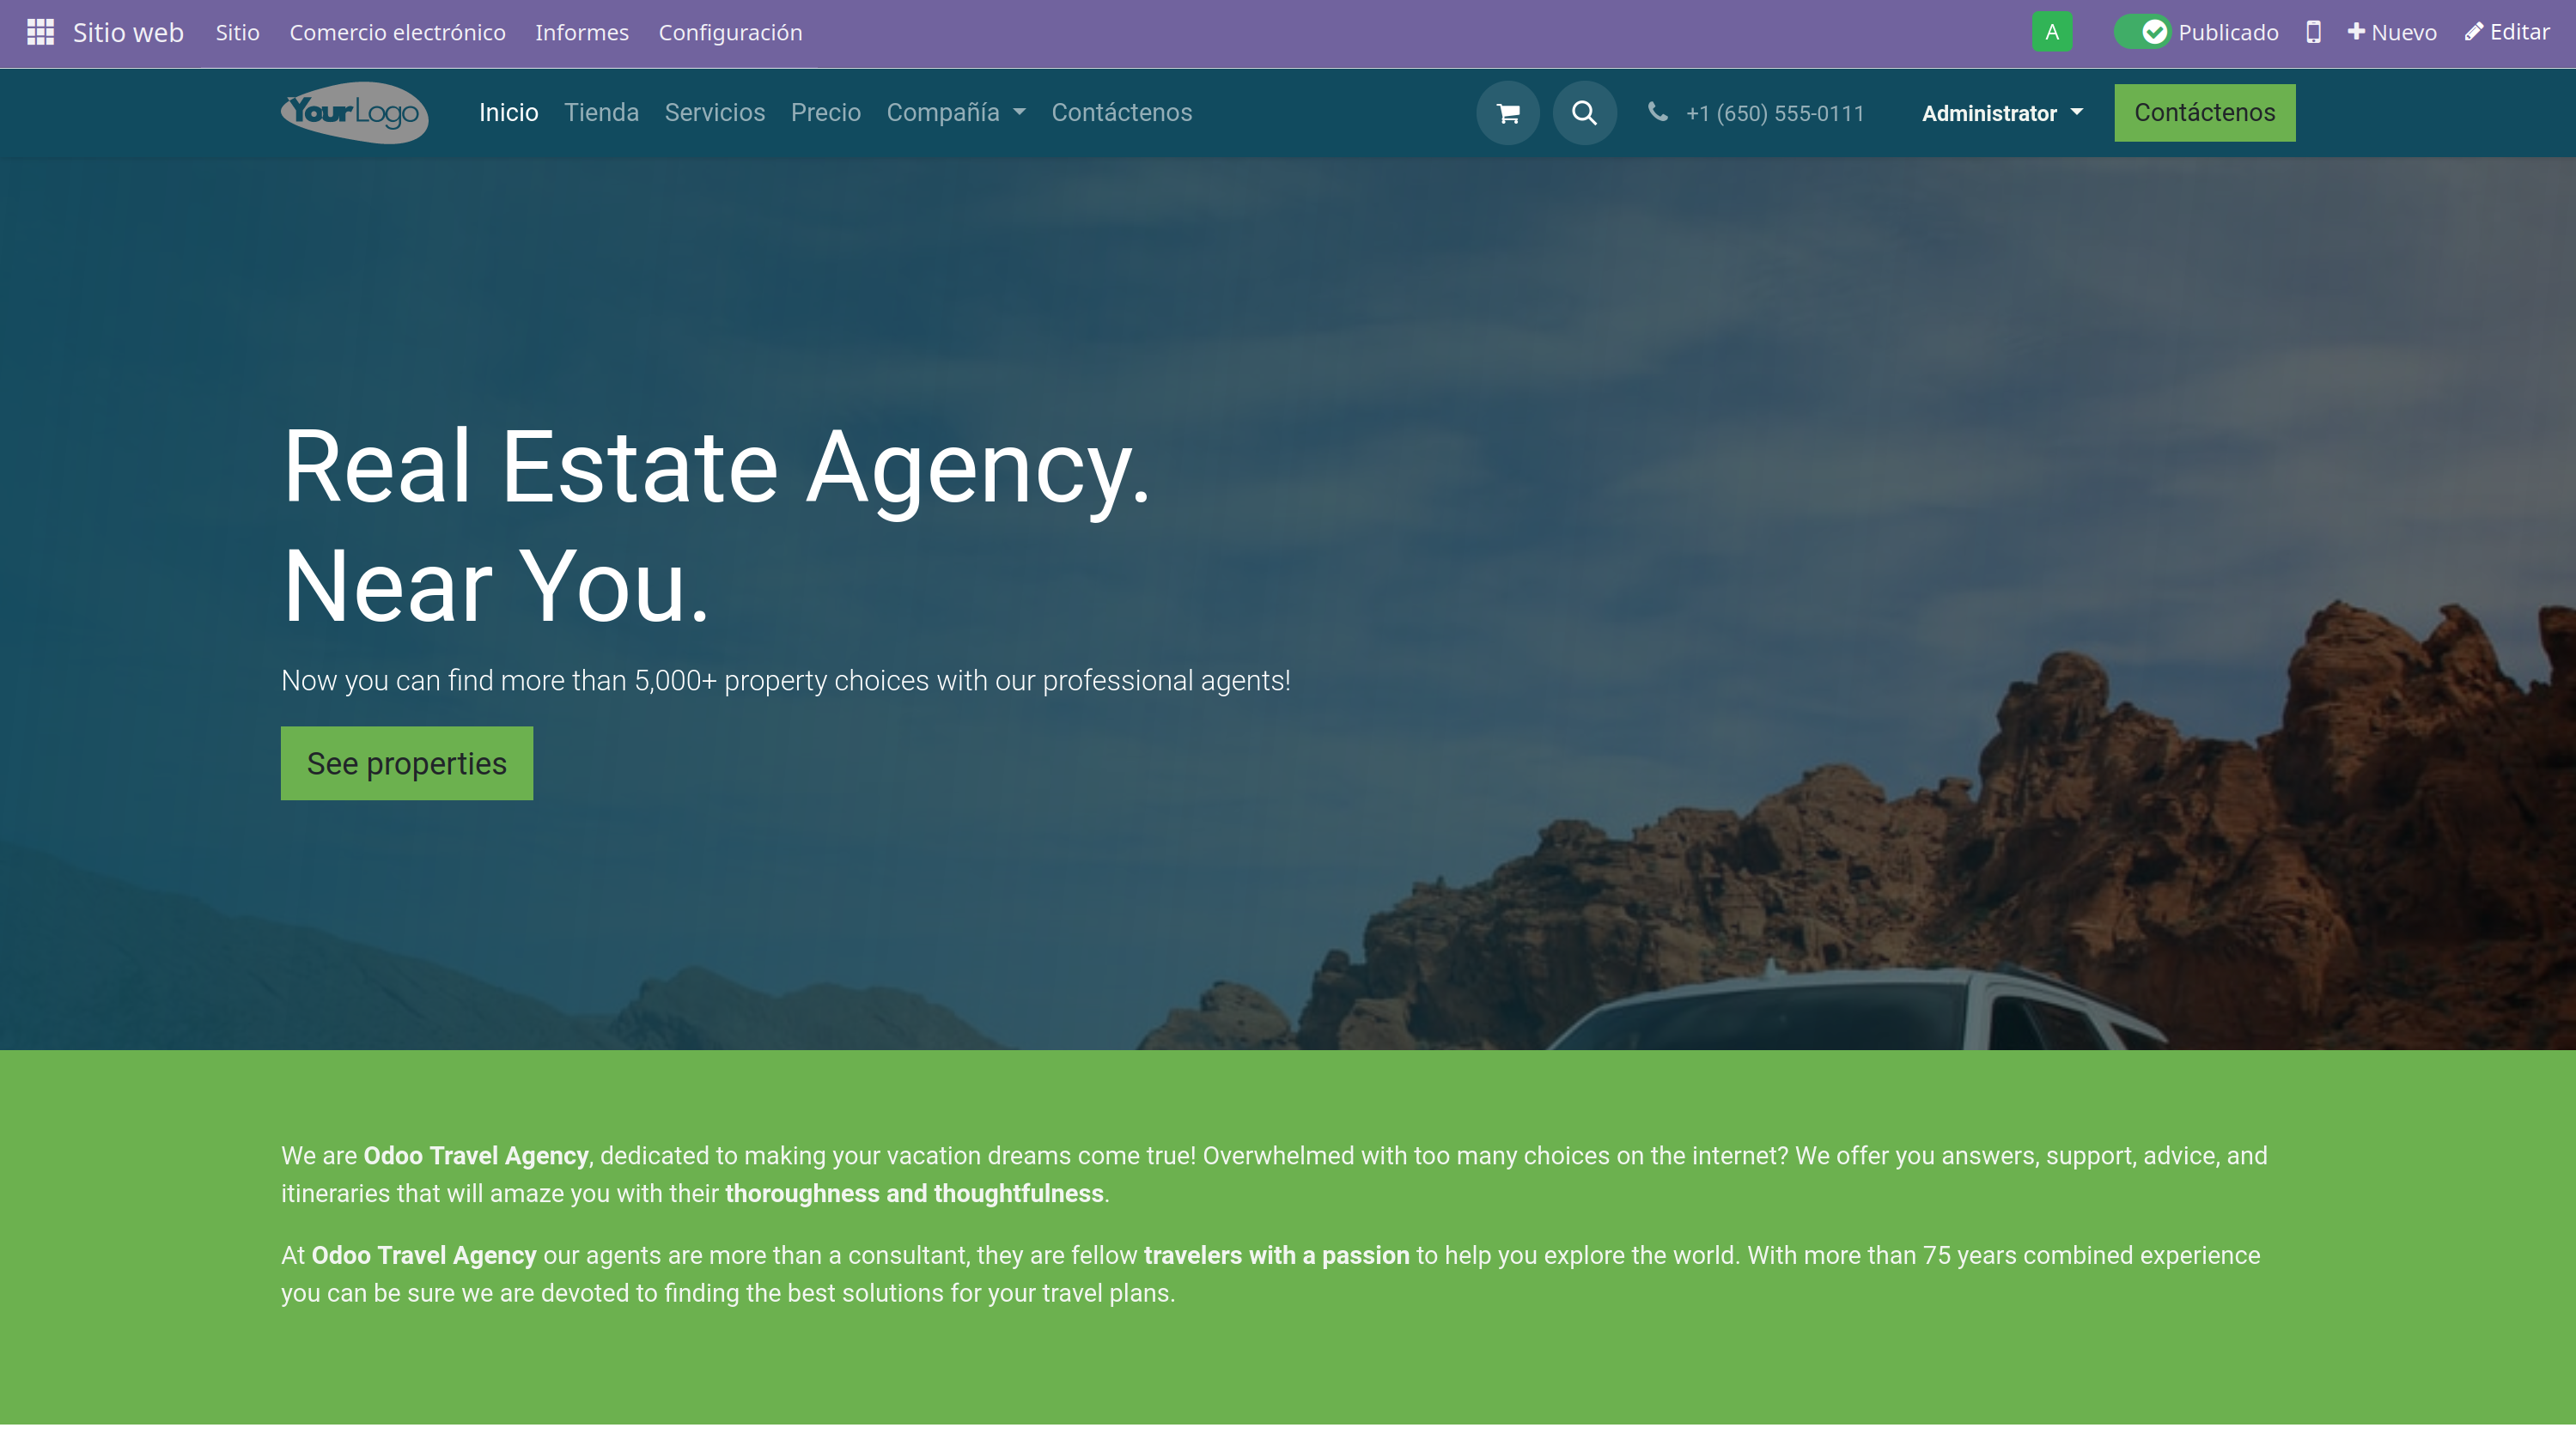
\includegraphics[width=6cm]{web.png}
    \caption{Sitio web creado automáticamente}
    \label{fig:web}
\end{figure}
Haz click en la opción Nuevo de la esquina superior derecha y selecciona Entrada de blog. Selecciona un blog existente o crea uno nuevo. Introduce el titulo de la entrada de blog y pulse guardar. Se mostrará la entrada de blog creada y un menú donde editar esta vista.
\paragraph{}
Si se clicka en el fondo verde que engloba el titulo se puede editar y añadir una imagen al fondo. Además, si se quiere añadir una galeria de fotos sobre el producto, en este caso el coche:
\begin{figure}[h]
    \centering
    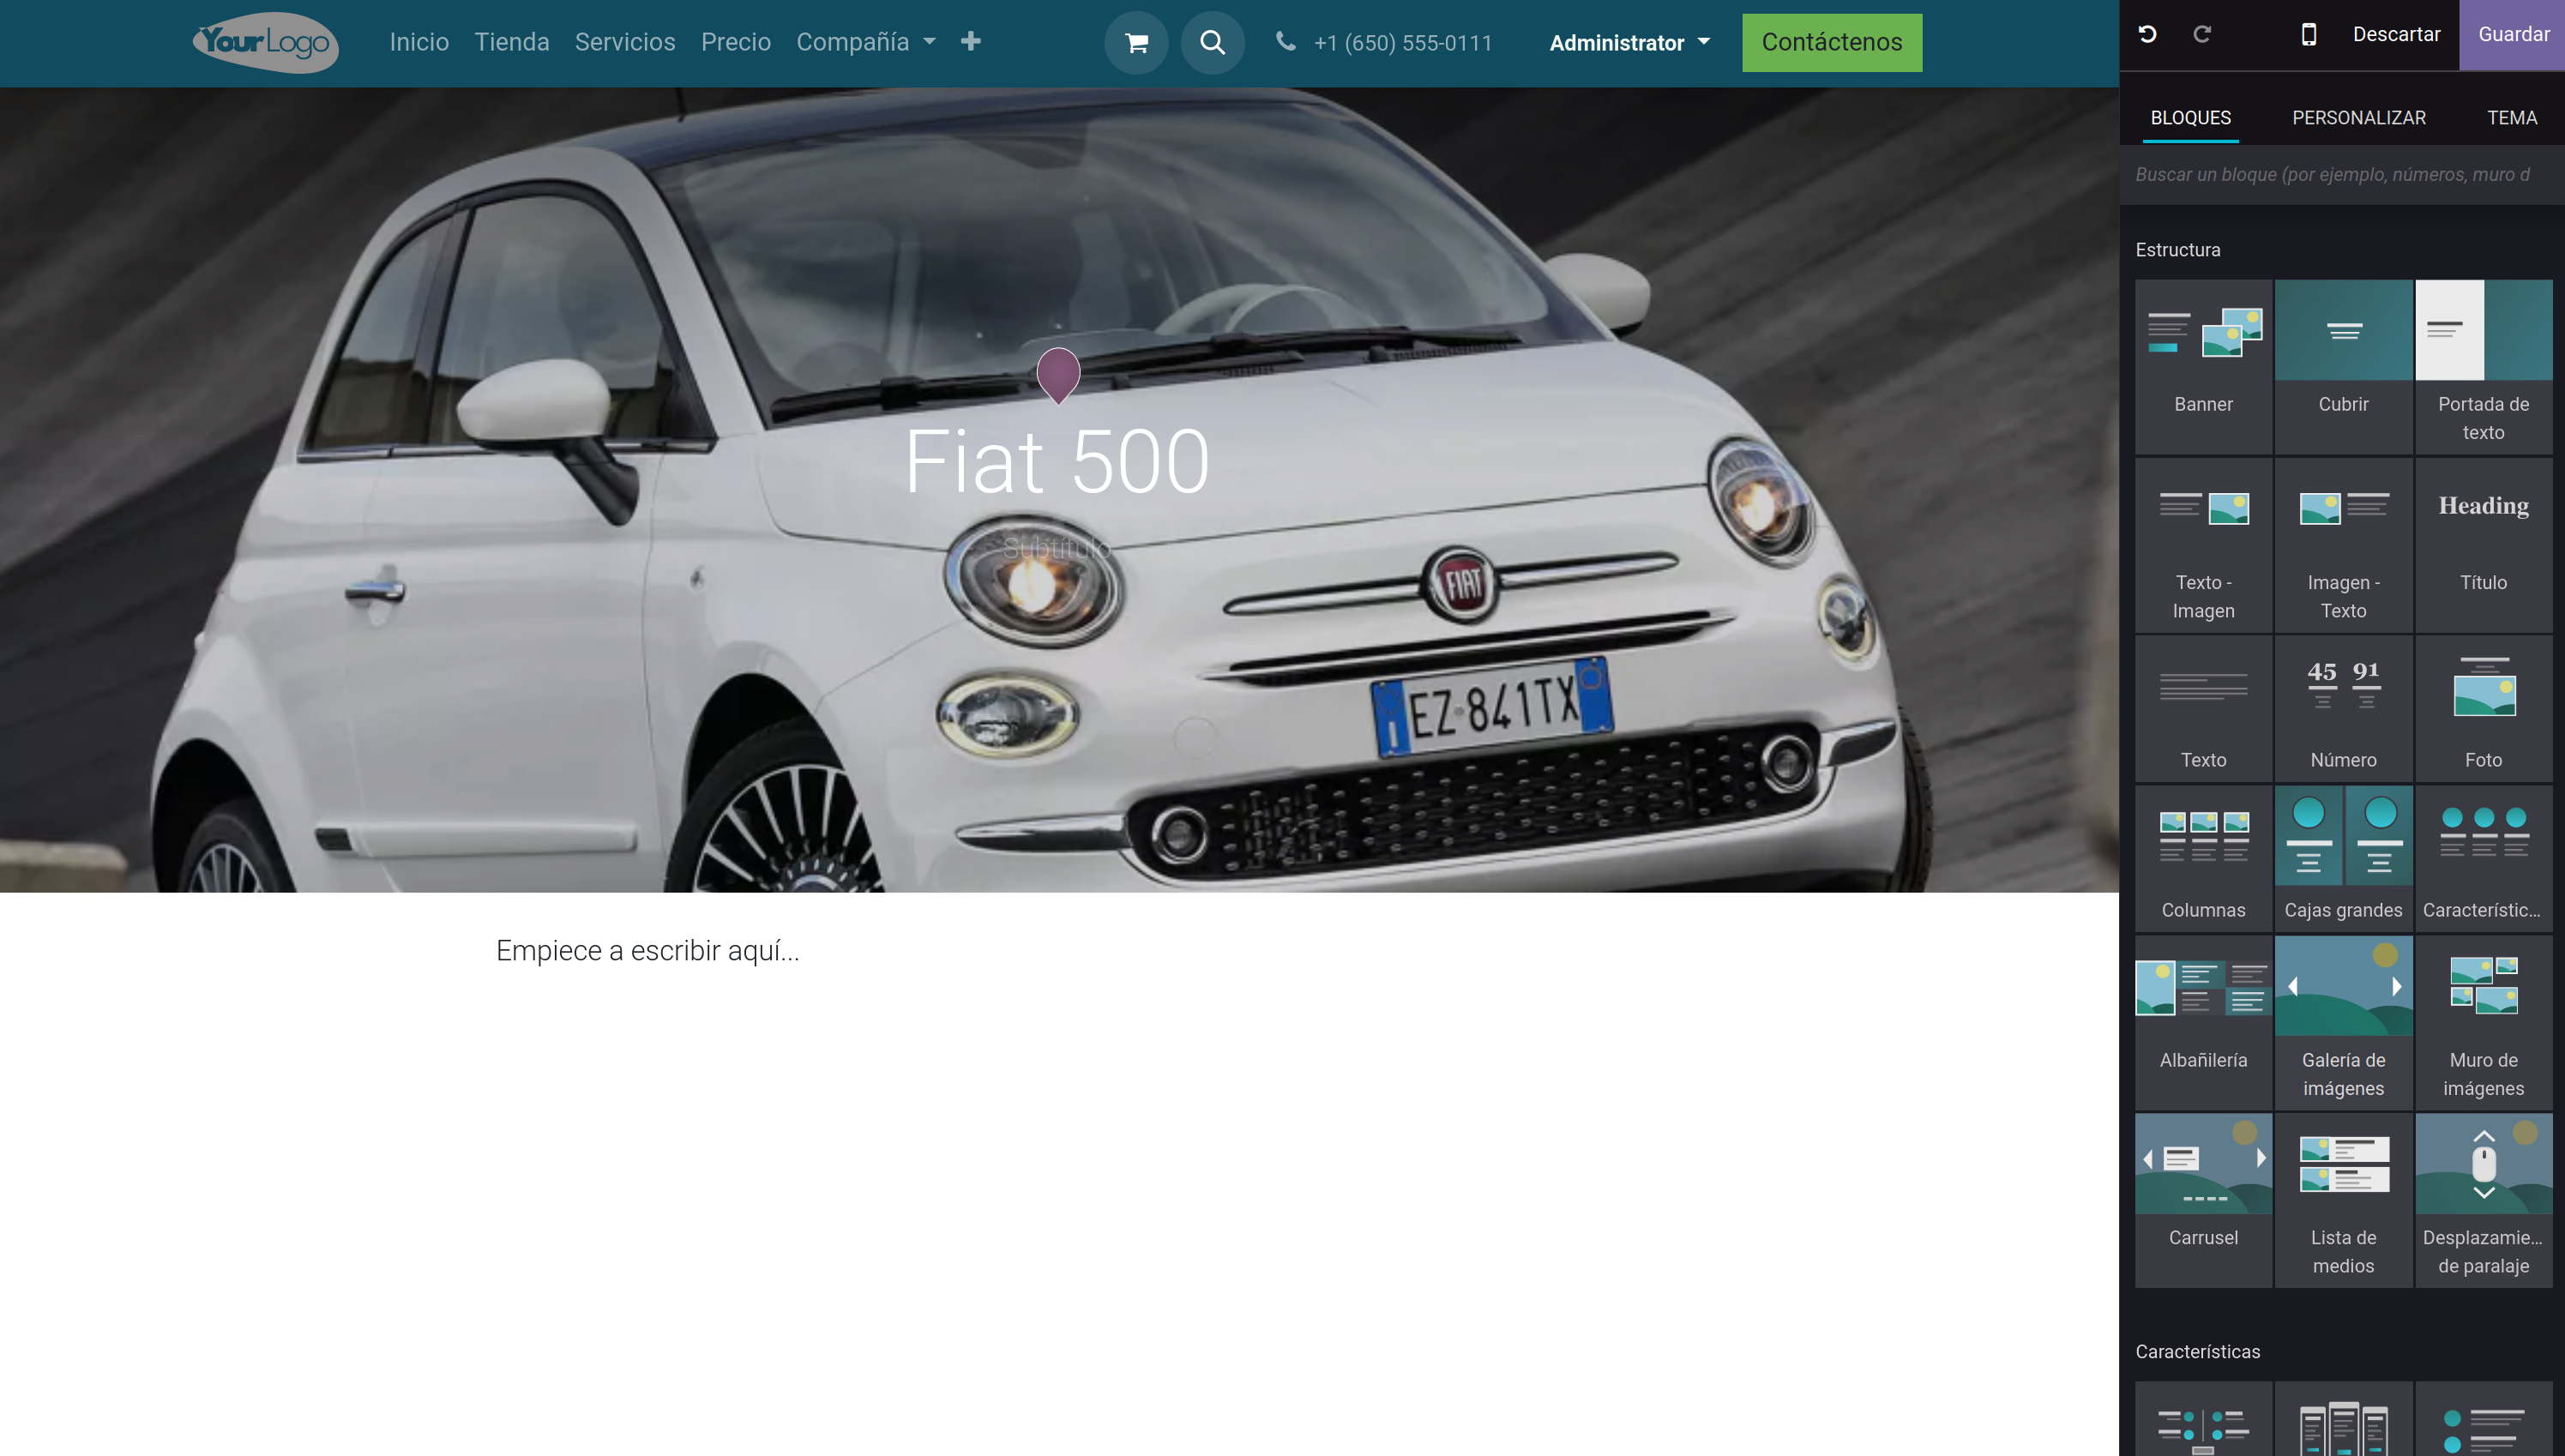
\includegraphics[width=6cm]{galeria.png}
    \caption{Adición de galería de fotos a la entrada de blog}
    \label{fig:galeria}
\end{figure}
Arrastra la galeria de imágenes del menú lateral derecho de edición y sueltalo en la parte de la web donde se quiere ubicar. Si haces click en la galeria, se mostrará un menu de edición en el lateral derecho donde se puede editar y personalizar. Para añadir las imagenes que se quieren mostrar se tendrá que dar click en Añadir en la opción de Imagenes dentro de la sección Galeria de imagenes del menú de edición. A continuación, hacer click en subir archivo y seleccionar las imagenes. Una vez subidas las fotos a Odoo, se hacer click en cada imagen de la galeria y se seleccionará la foto a mostrar. 
\paragraph{}
Si se quiere dar acceso a compra del producto mostrado se añadirá un bloque llamado Llamamiento a la acción de la misma manera que se ha hecho la galería de imágenes. Además, se puede editar cualquier texto de la web, para adecuar la información a las necesidades.
\begin{figure}[h]
    \centering
    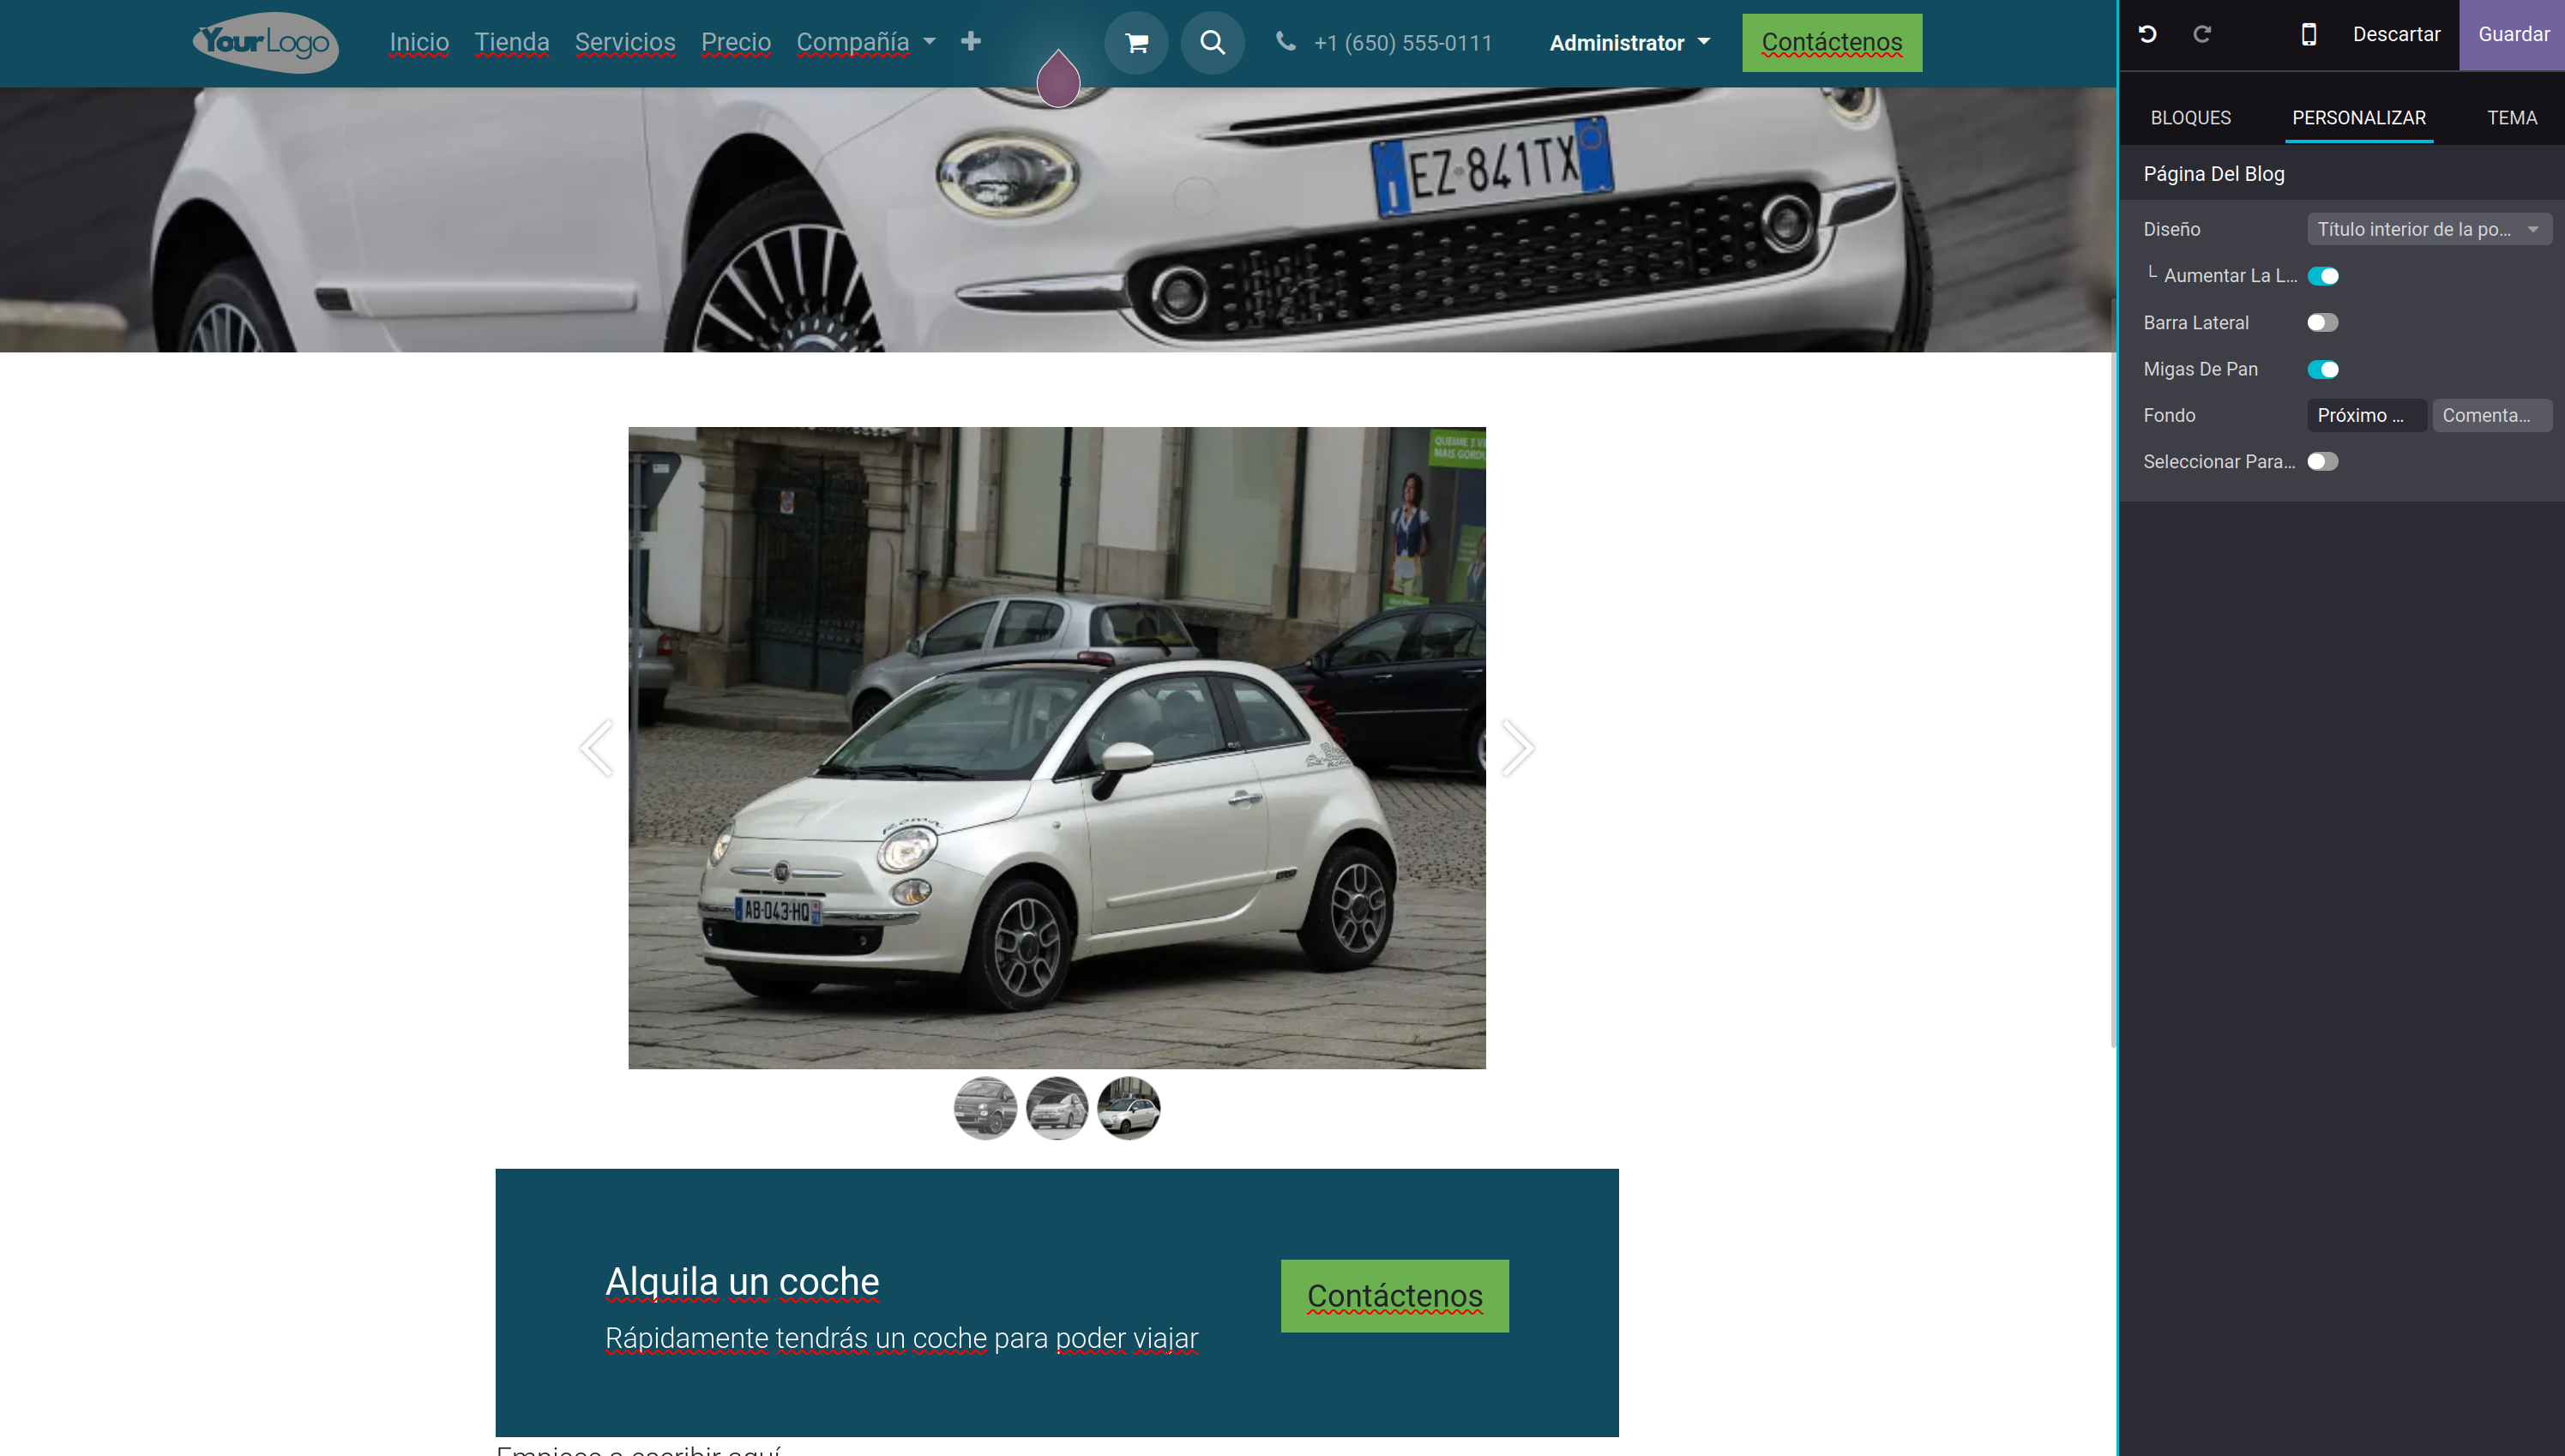
\includegraphics[width=6cm]{callToAction.png}
    \caption{Adición de un llamamiento a la acción a la entrada de blog}
    \label{fig:callToAction}
\end{figure}
Una vez, la entrada de blog esté a su gusto guárdalo clickando en el botón guardar de la esquina superior derecha.
\paragraph{}
Para añadir una página nueva al sitio web añadimos una página como en la figura 4. Selecciona la opción Servicios del menu lateral izquierdo y elige la página que más se adecua a las necesidades, en este caso se va a crear un sitio donde están las preguntas frecuentes, problemas comunes y sus soluciones, por lo que se va a elegir la segunda opción.
\begin{figure}[h]
    \centering
    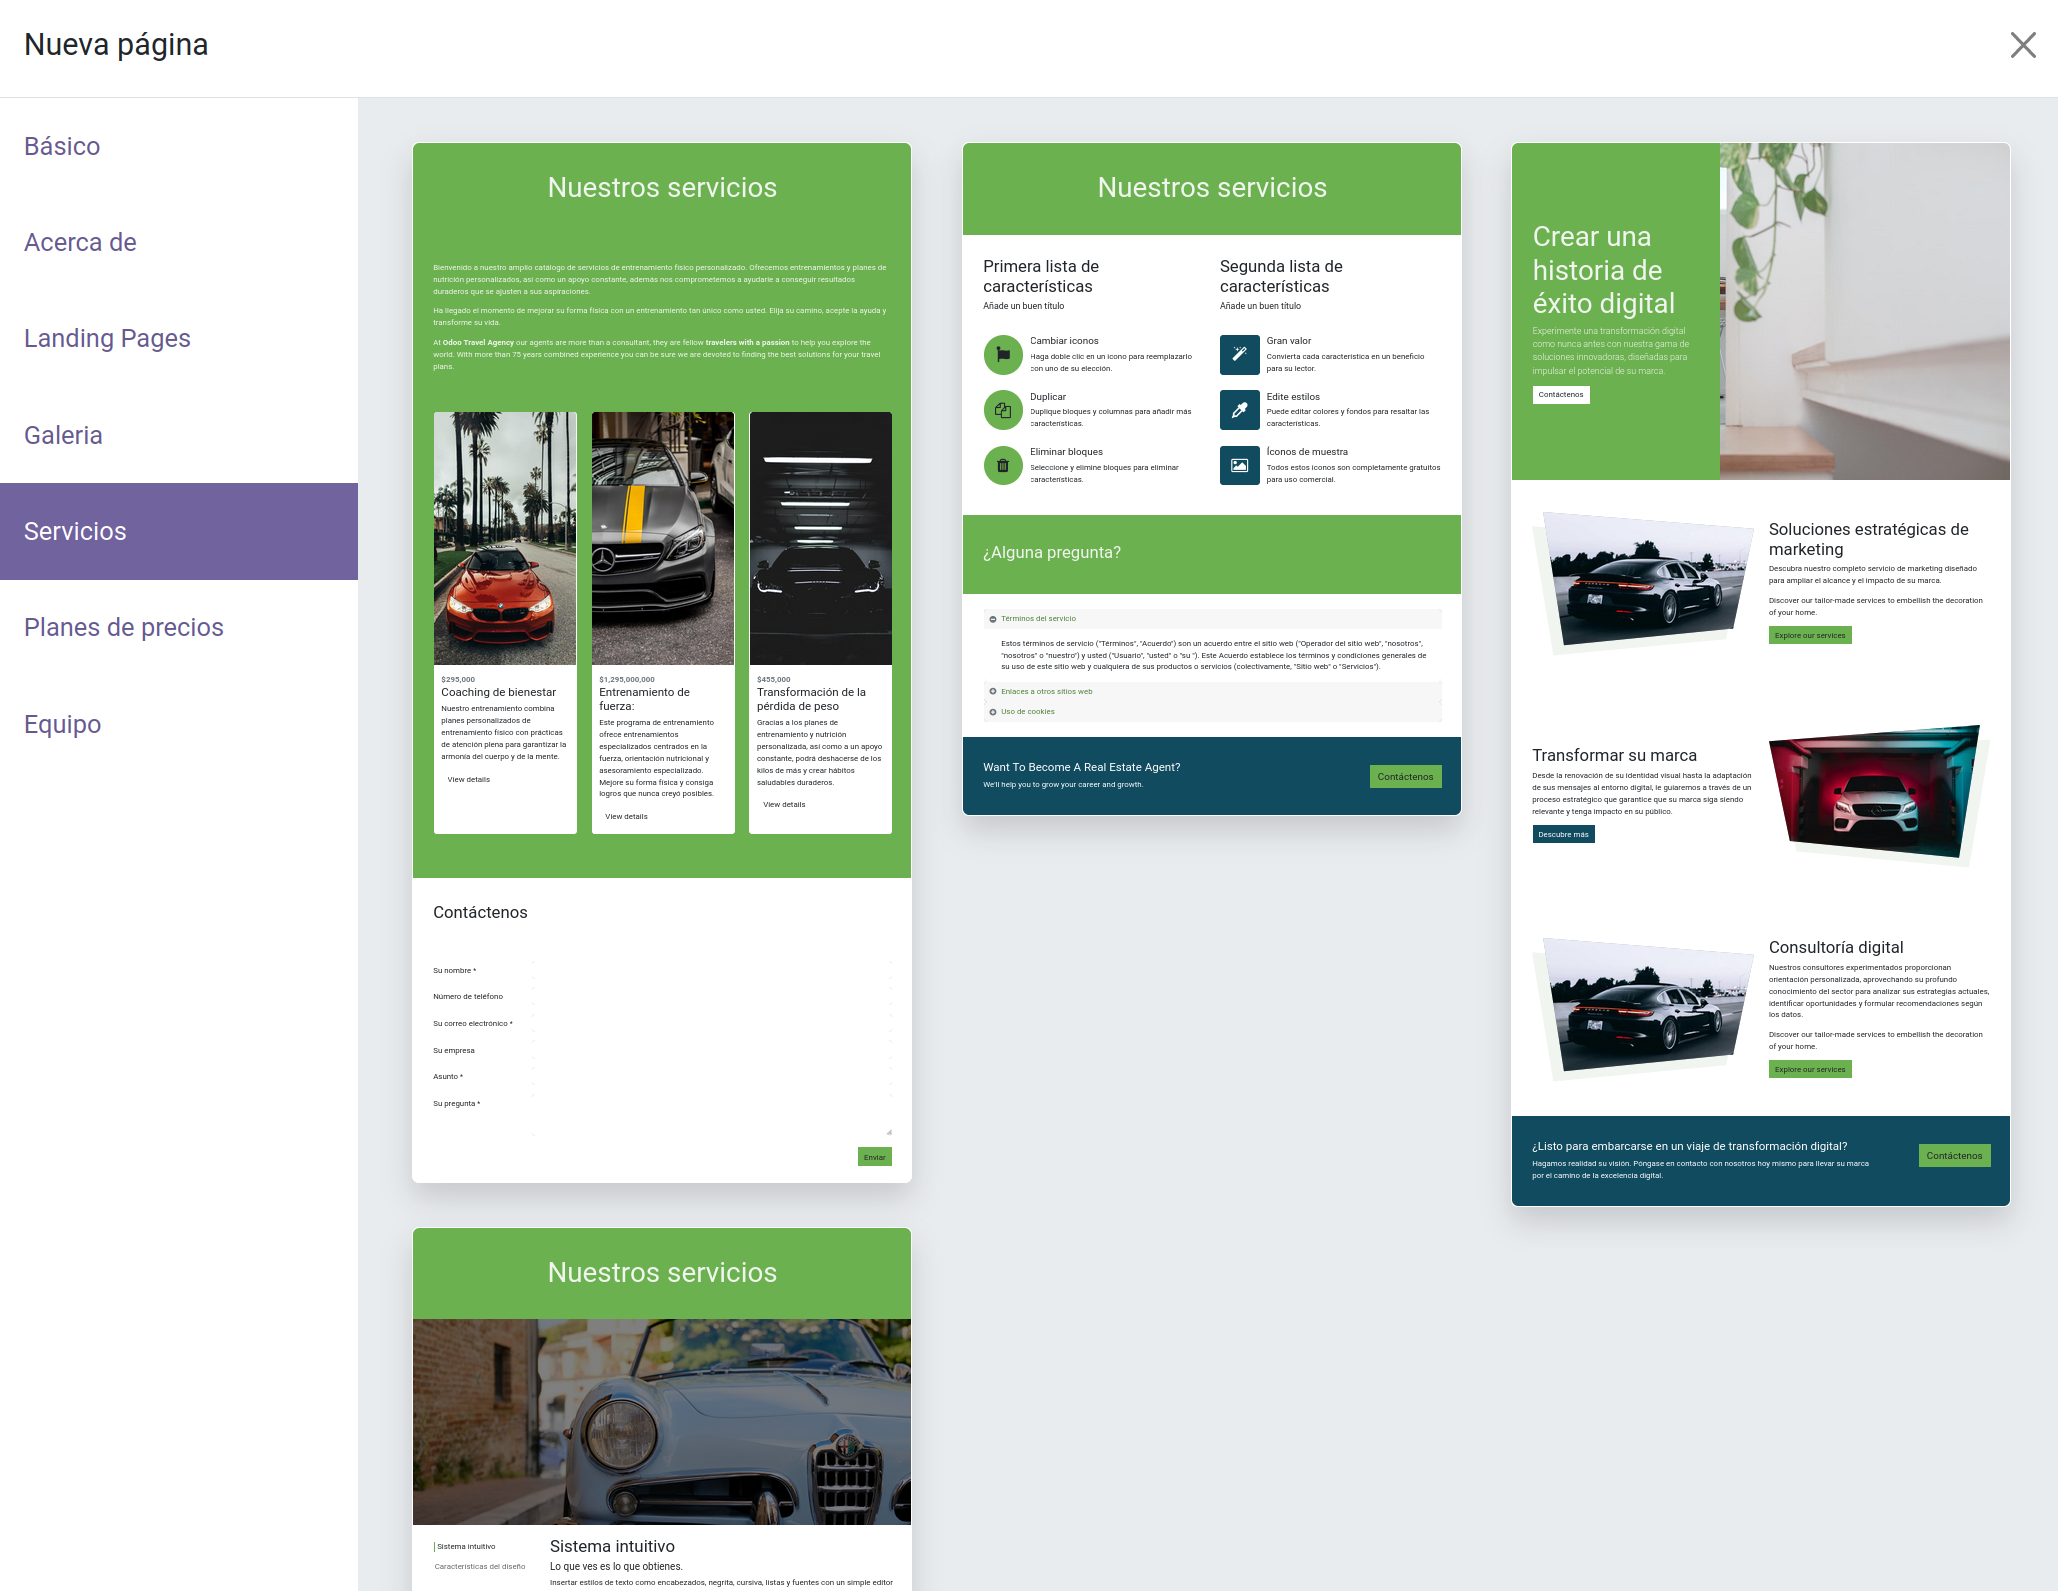
\includegraphics[width=6cm]{addPagina.png}
    \caption{Creación de una página para mostrar FAQs}
    \label{fig:addPagina}
\end{figure}
Introduce el titulo de la página, deja activada la opción de Añadir al menú y pulsa en crear.
\begin{figure}[h]
    \centering
    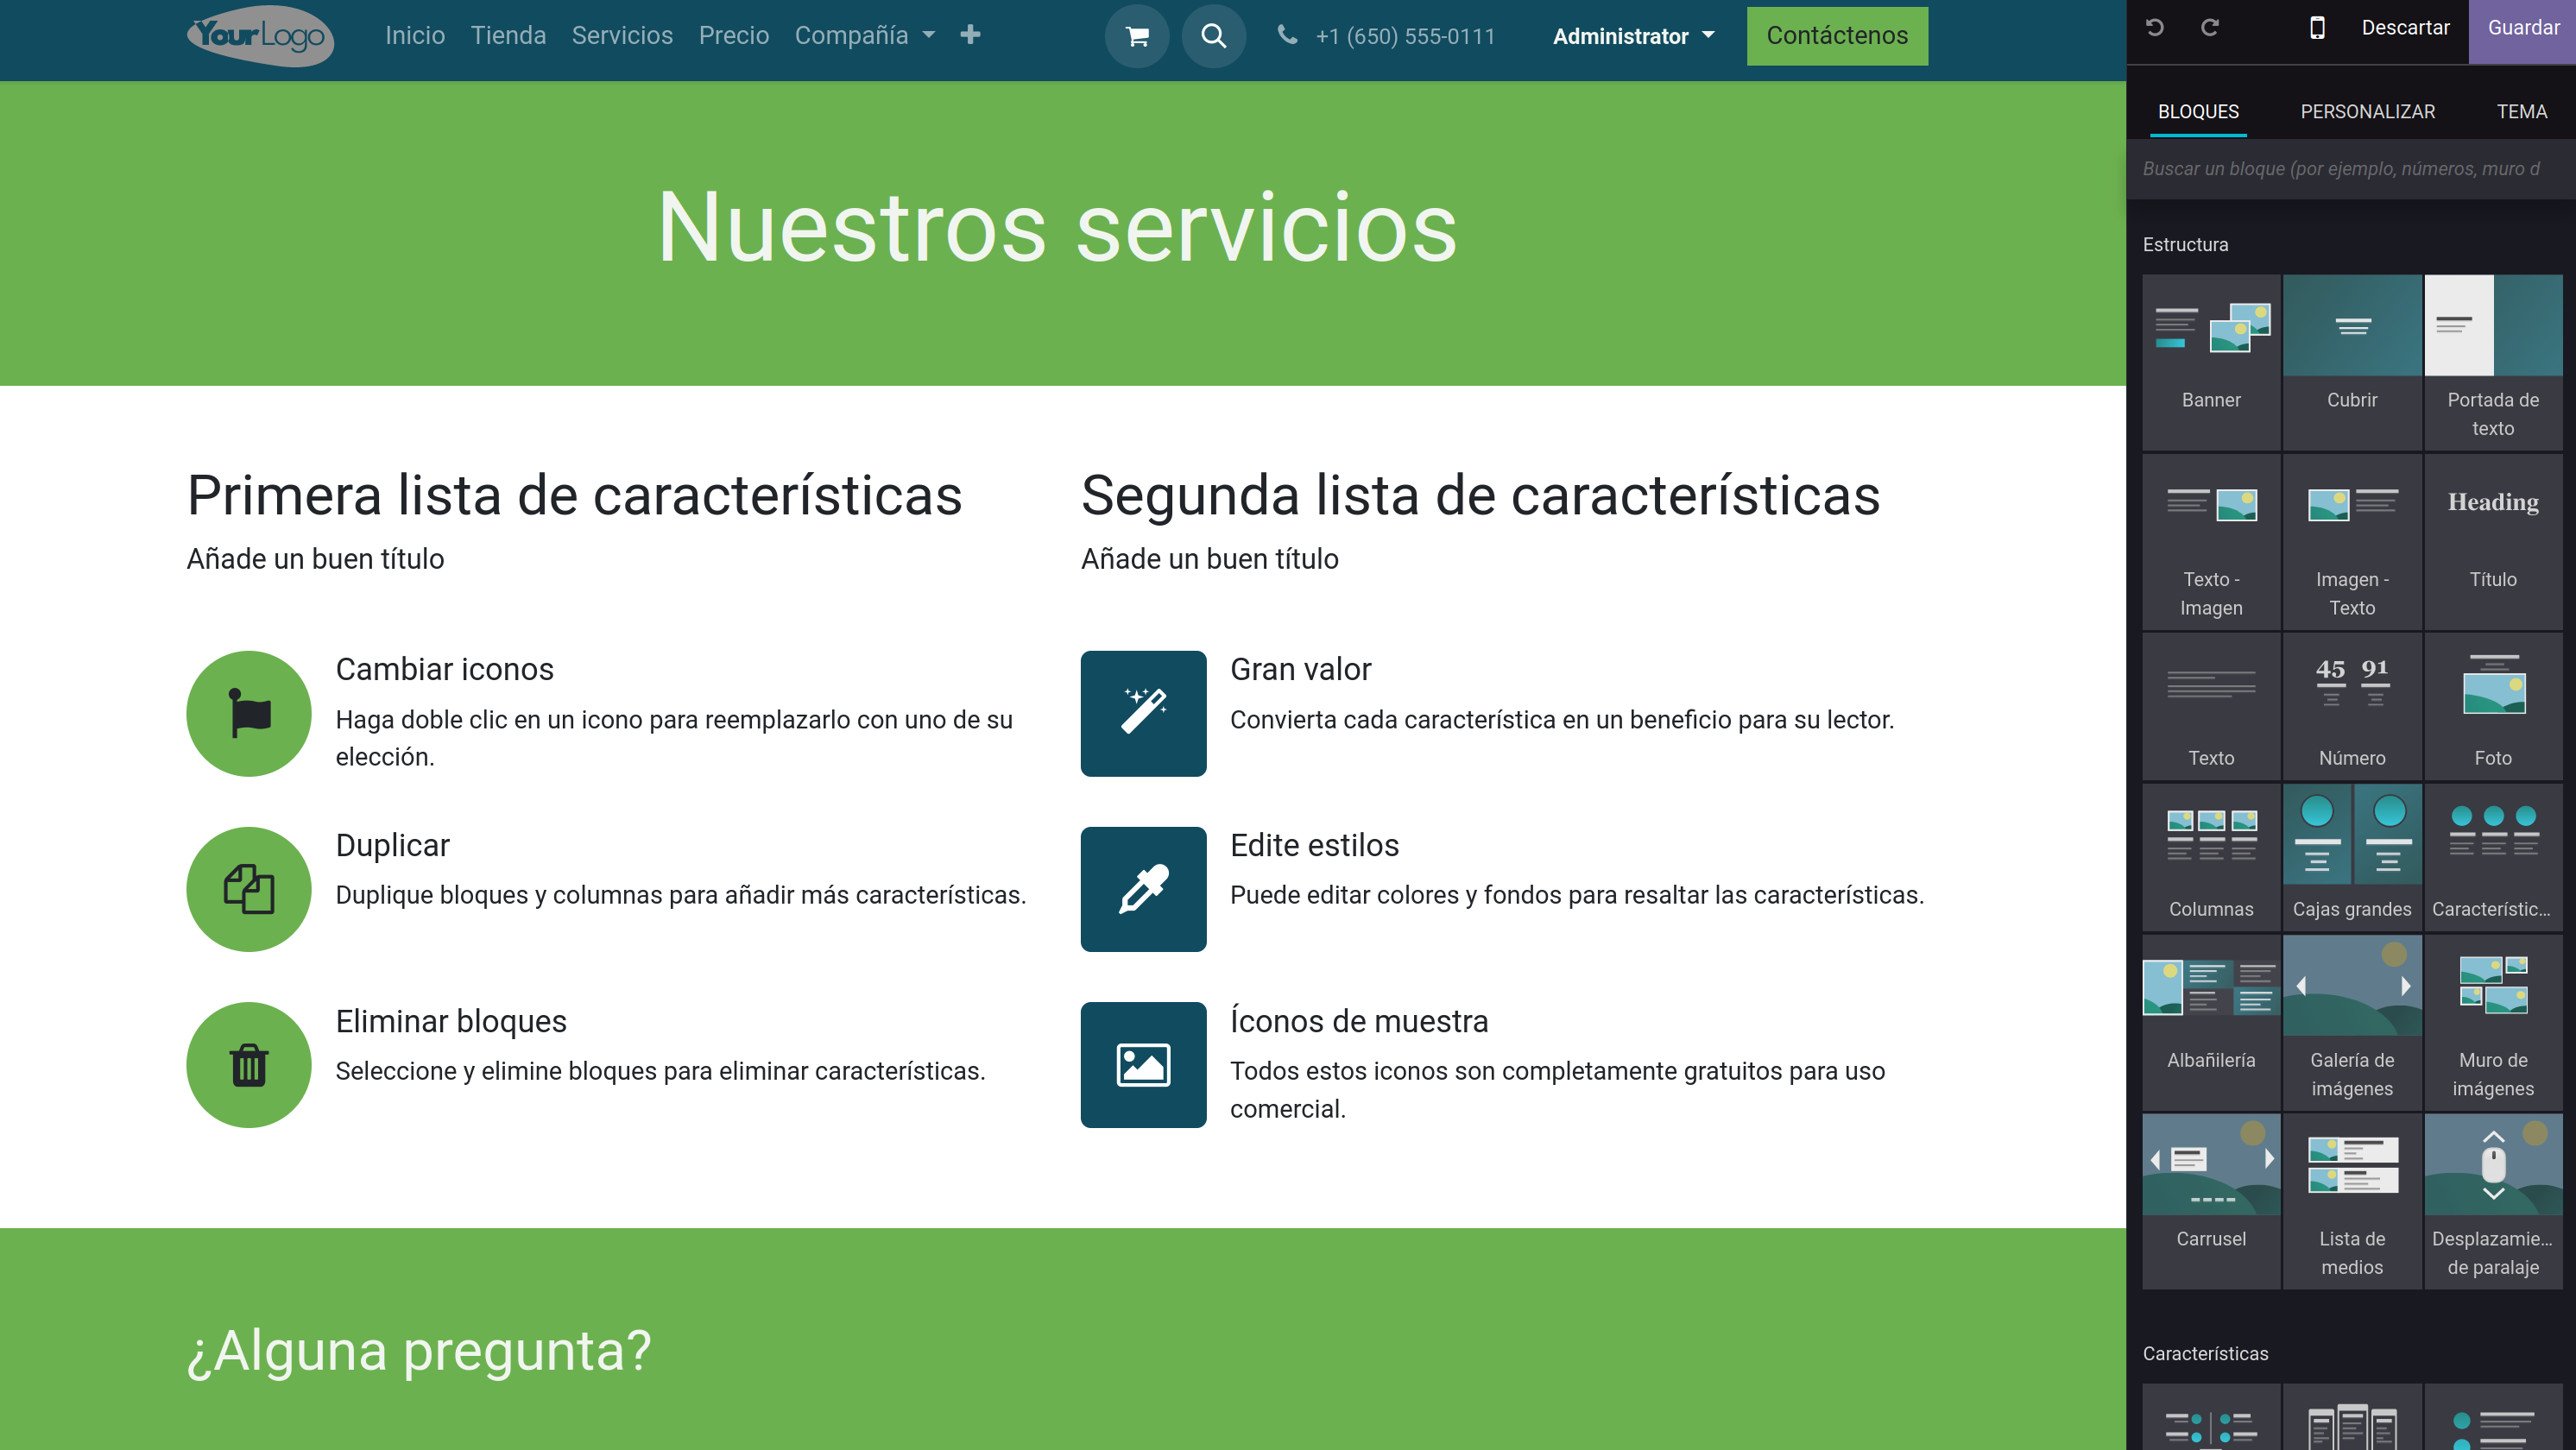
\includegraphics[width=6cm]{paginaNueva.png}
    \caption{Página para mostrar FAQs creada}
    \label{fig:paginaNueva}
\end{figure}
Como ya hemos explicado anteriormente, edita y personaliza cada texto y foto para que se ajuste a las necesidades propias. Vamos a centrarnos en el contenido importante de esta página que son las preguntas y problemas frecuentes y como solucionarlo. Para ello, se va a utilizar el bloque acordeón que ya existe en la parte inferior de la página. Para añadir nuevos temas clica encima del acordeón y clica en Añadir Artículo de la opción Tema de la sección Acordeón del menú lateral derecho. Se añadirá un nuevo artículo al final del acordeón, selecciona cada texto para incluir la información personalizada y selecciona la opción junto a la basura, para arrastrar el artículo y ordenarlos dentro del acordeón.
\begin{figure}[h]
    \centering
    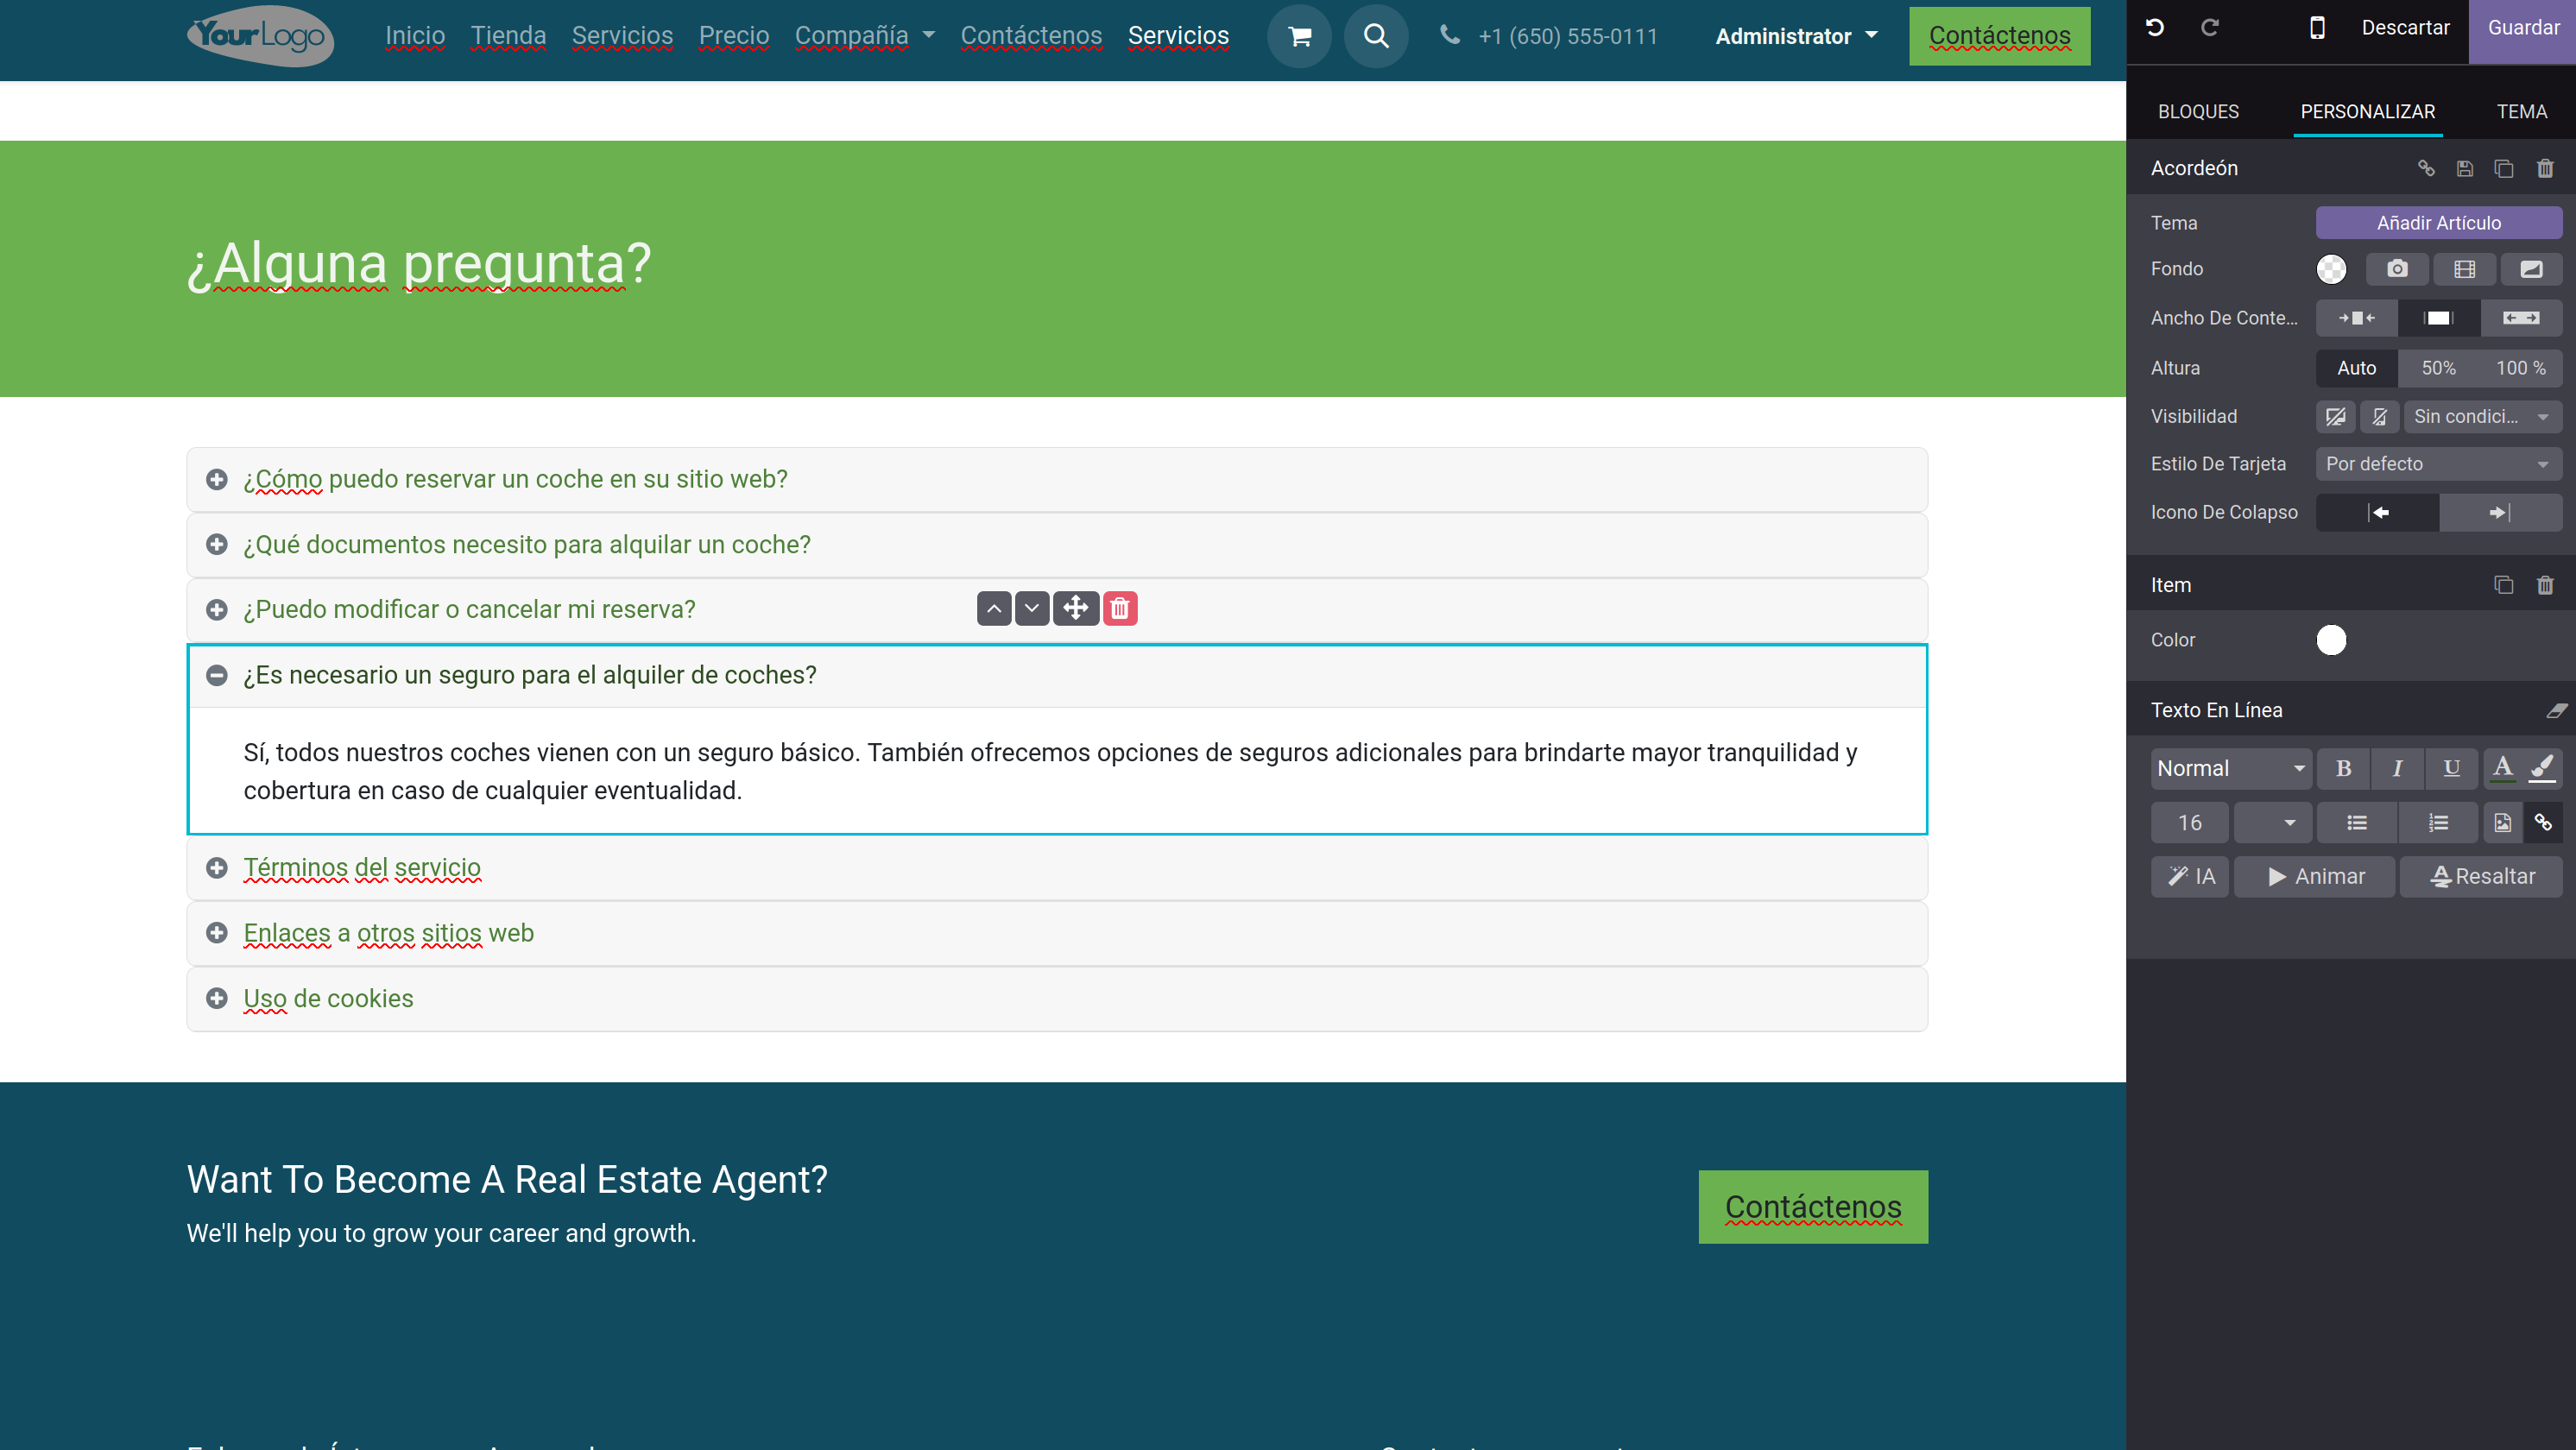
\includegraphics[width=6cm]{faqs.png}
    \caption{Creando el acordeón con los FAQs}
    \label{fig:faqs}
\end{figure}
Finalmente, haz click en guardar en la esquina superior derecha.
\section{Configuración funcional}
\paragraph{}
A continuación, se va a llevar a cabo la configuración funcional de Odoo. Para ello se va a explicar paso a paso el proceso de creación de una compañía. Primero, se debe ir al menú de configuración dentro de las opciones generales. Se hace click en el link Administrar compañías.
\newpage
\begin{figure}[h]
    \centering
    \includegraphics[width=6cm]{adminCompañias.png}
    \caption{Página de configuración de opciones generales}
    \label{fig:faqs}
\end{figure}
Luego en la esquina superior izquierda selecciona el botón New. Se llegará al menú de creación de una compañía.
\begin{figure}[h]
    \centering
    \includegraphics[width=6cm]{crearCompañias.png}
    \caption{Creando una nueva compañía}
    \label{fig:faqs}
\end{figure}
\paragraph{}
Introduce los datos correspondientes a la compañía que se quiere crear. Por último, si navegas hacia atrás a la página de administración de las compañías verás que se ha creado una nueva. Además, si se quieren crear compañías en otros países que sean ramas de una compañía matriz, se debe seleccionar desde la página de administración de compañías la compañía que se quiere que sea la matriz. Se entra en el menú Ramas donde se puede administrar las compañías ramas. 
\begin{figure}[h]
    \centering
    \includegraphics[width=6cm]{ramasCompañias.png}
    \caption{Página de administración de compañías rama.}
    \label{fig:faqs}
\end{figure}
\paragraph{}
Para crear una compañía rama pulsa en la opción Agregar línea y rellena la información correspondiente. 
\newpage
\begin{figure}[h]
    \centering
    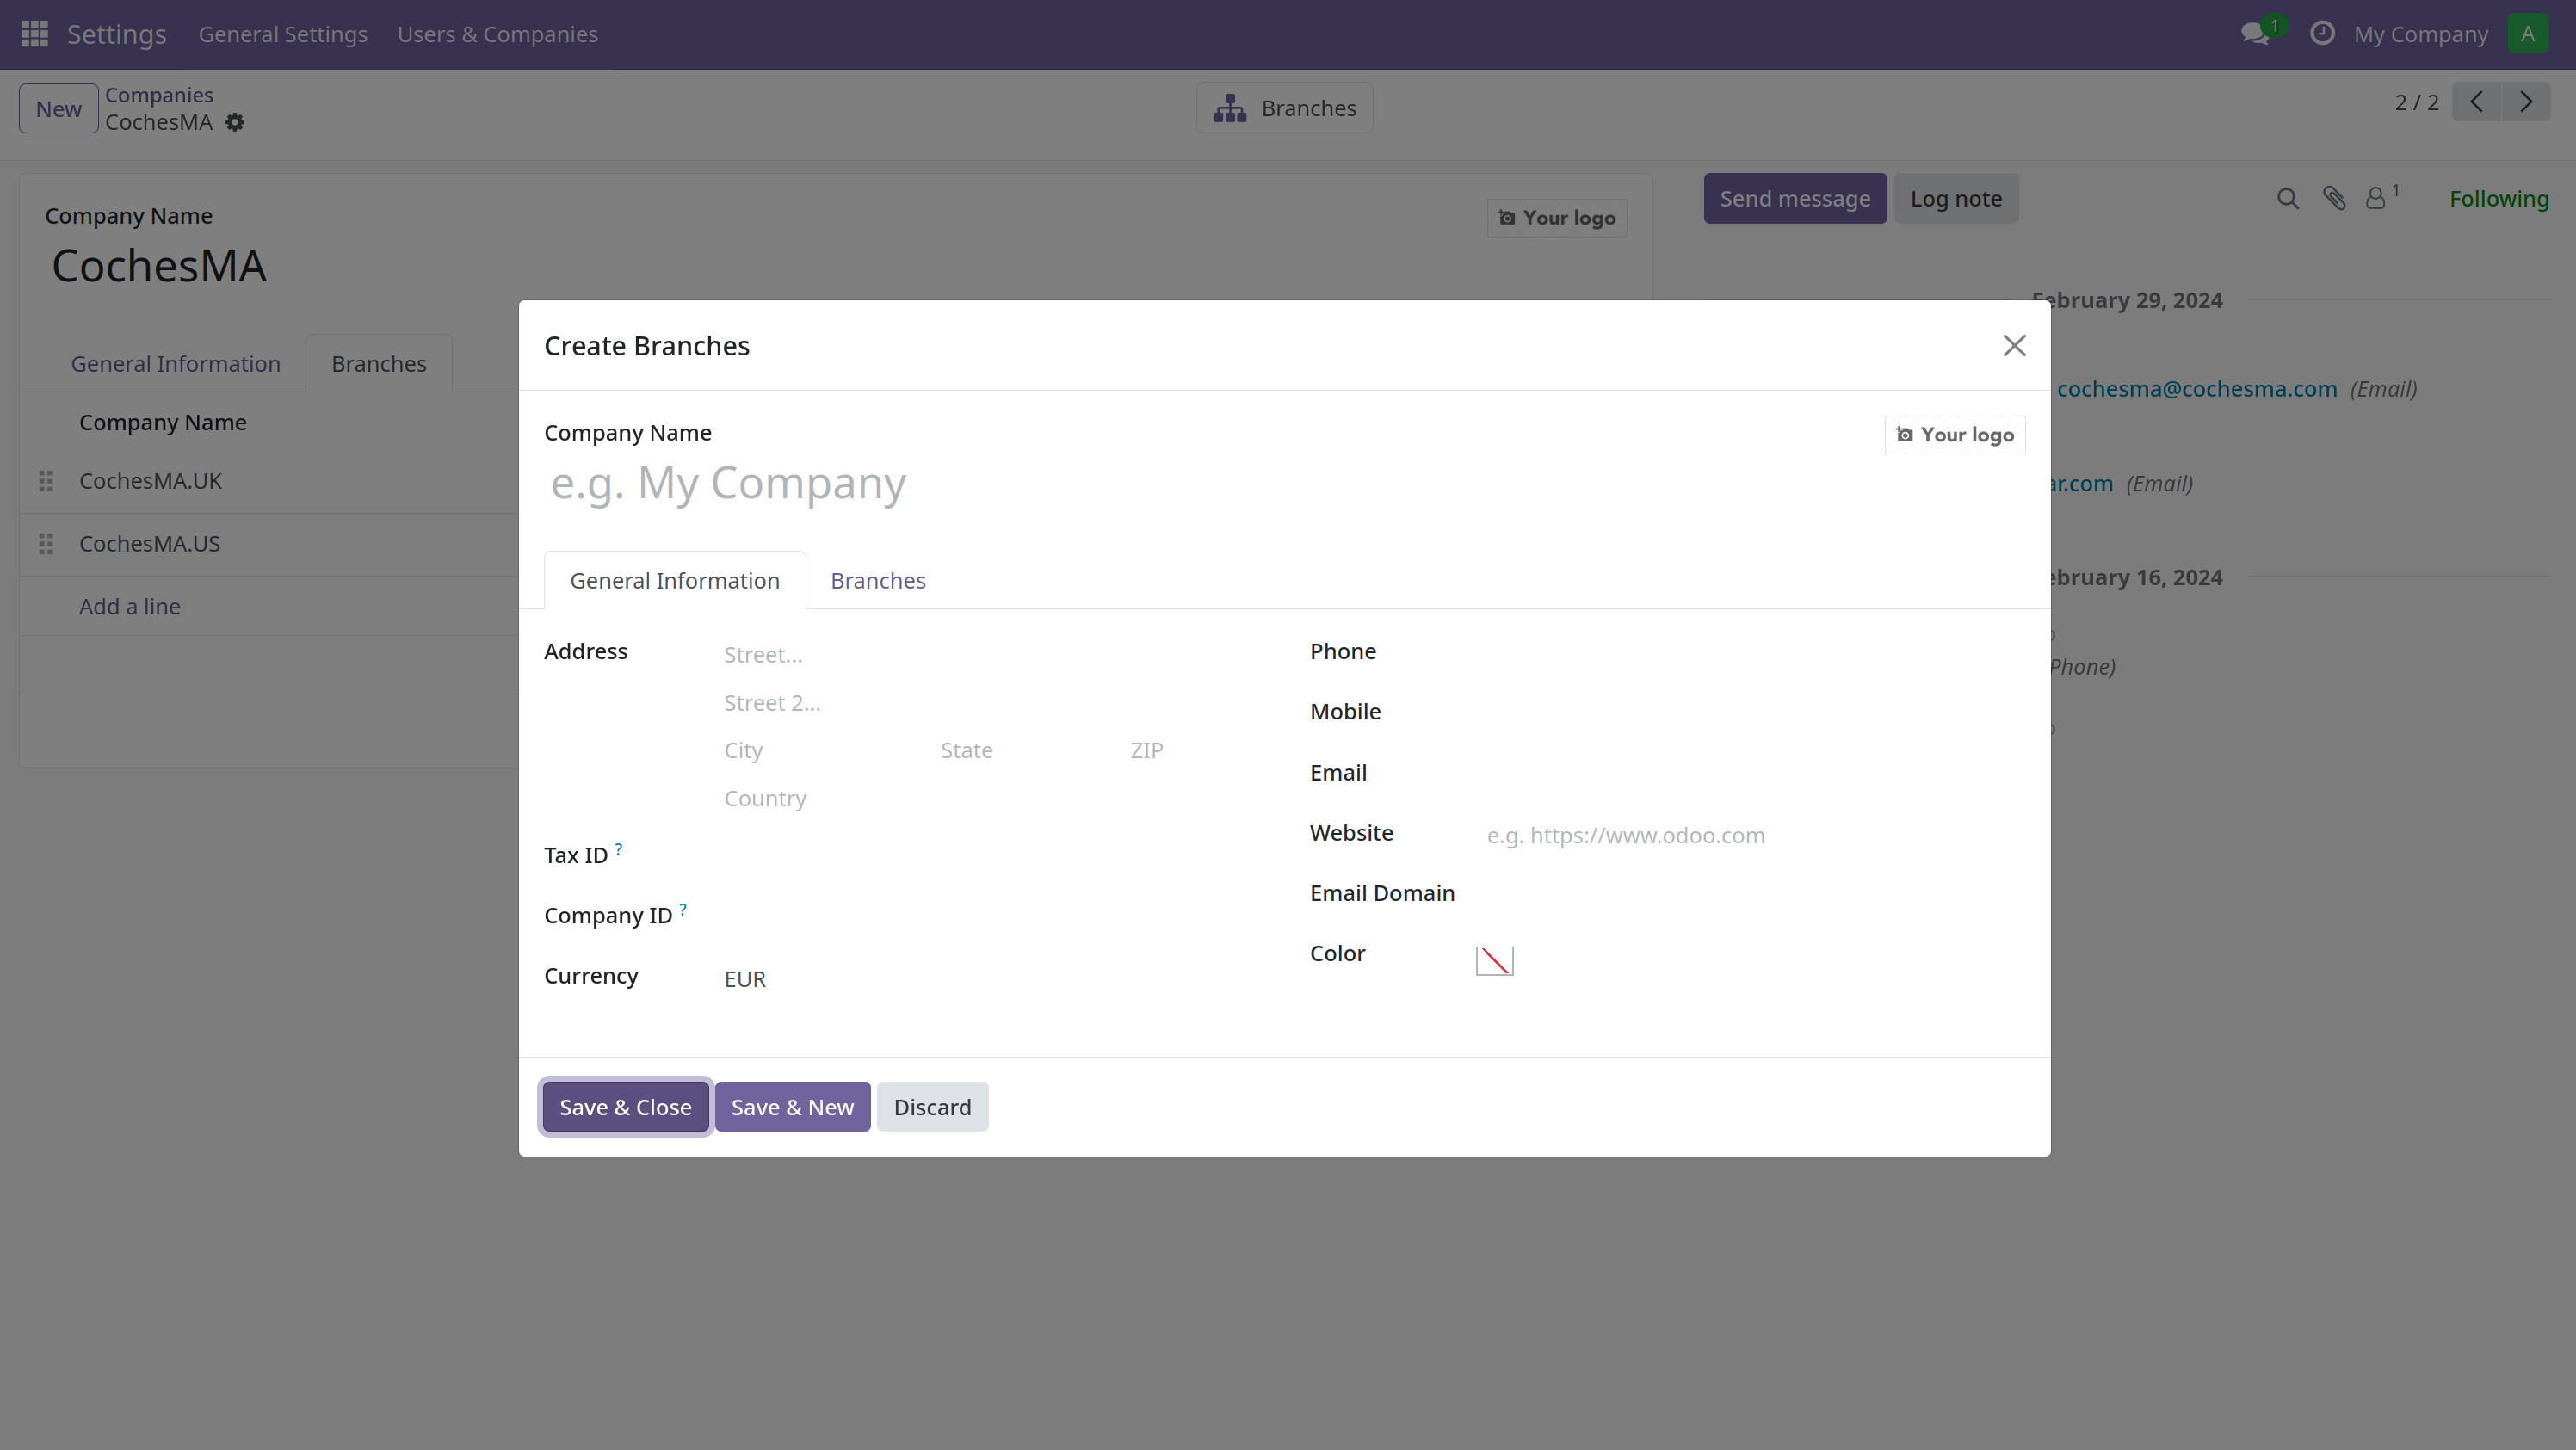
\includegraphics[width=6cm]{crearRama.png}
    \caption{Página de creación de compañías rama.}
    \label{fig:faqs}
\end{figure}
\paragraph{}
Una vez, introducido la información pulsa en Save and Close y se creará la empresa rama, podrás observar que ha aparecido una nueva rama en la página de administración de compañías rama.
\begin{figure}[h]
    \centering
    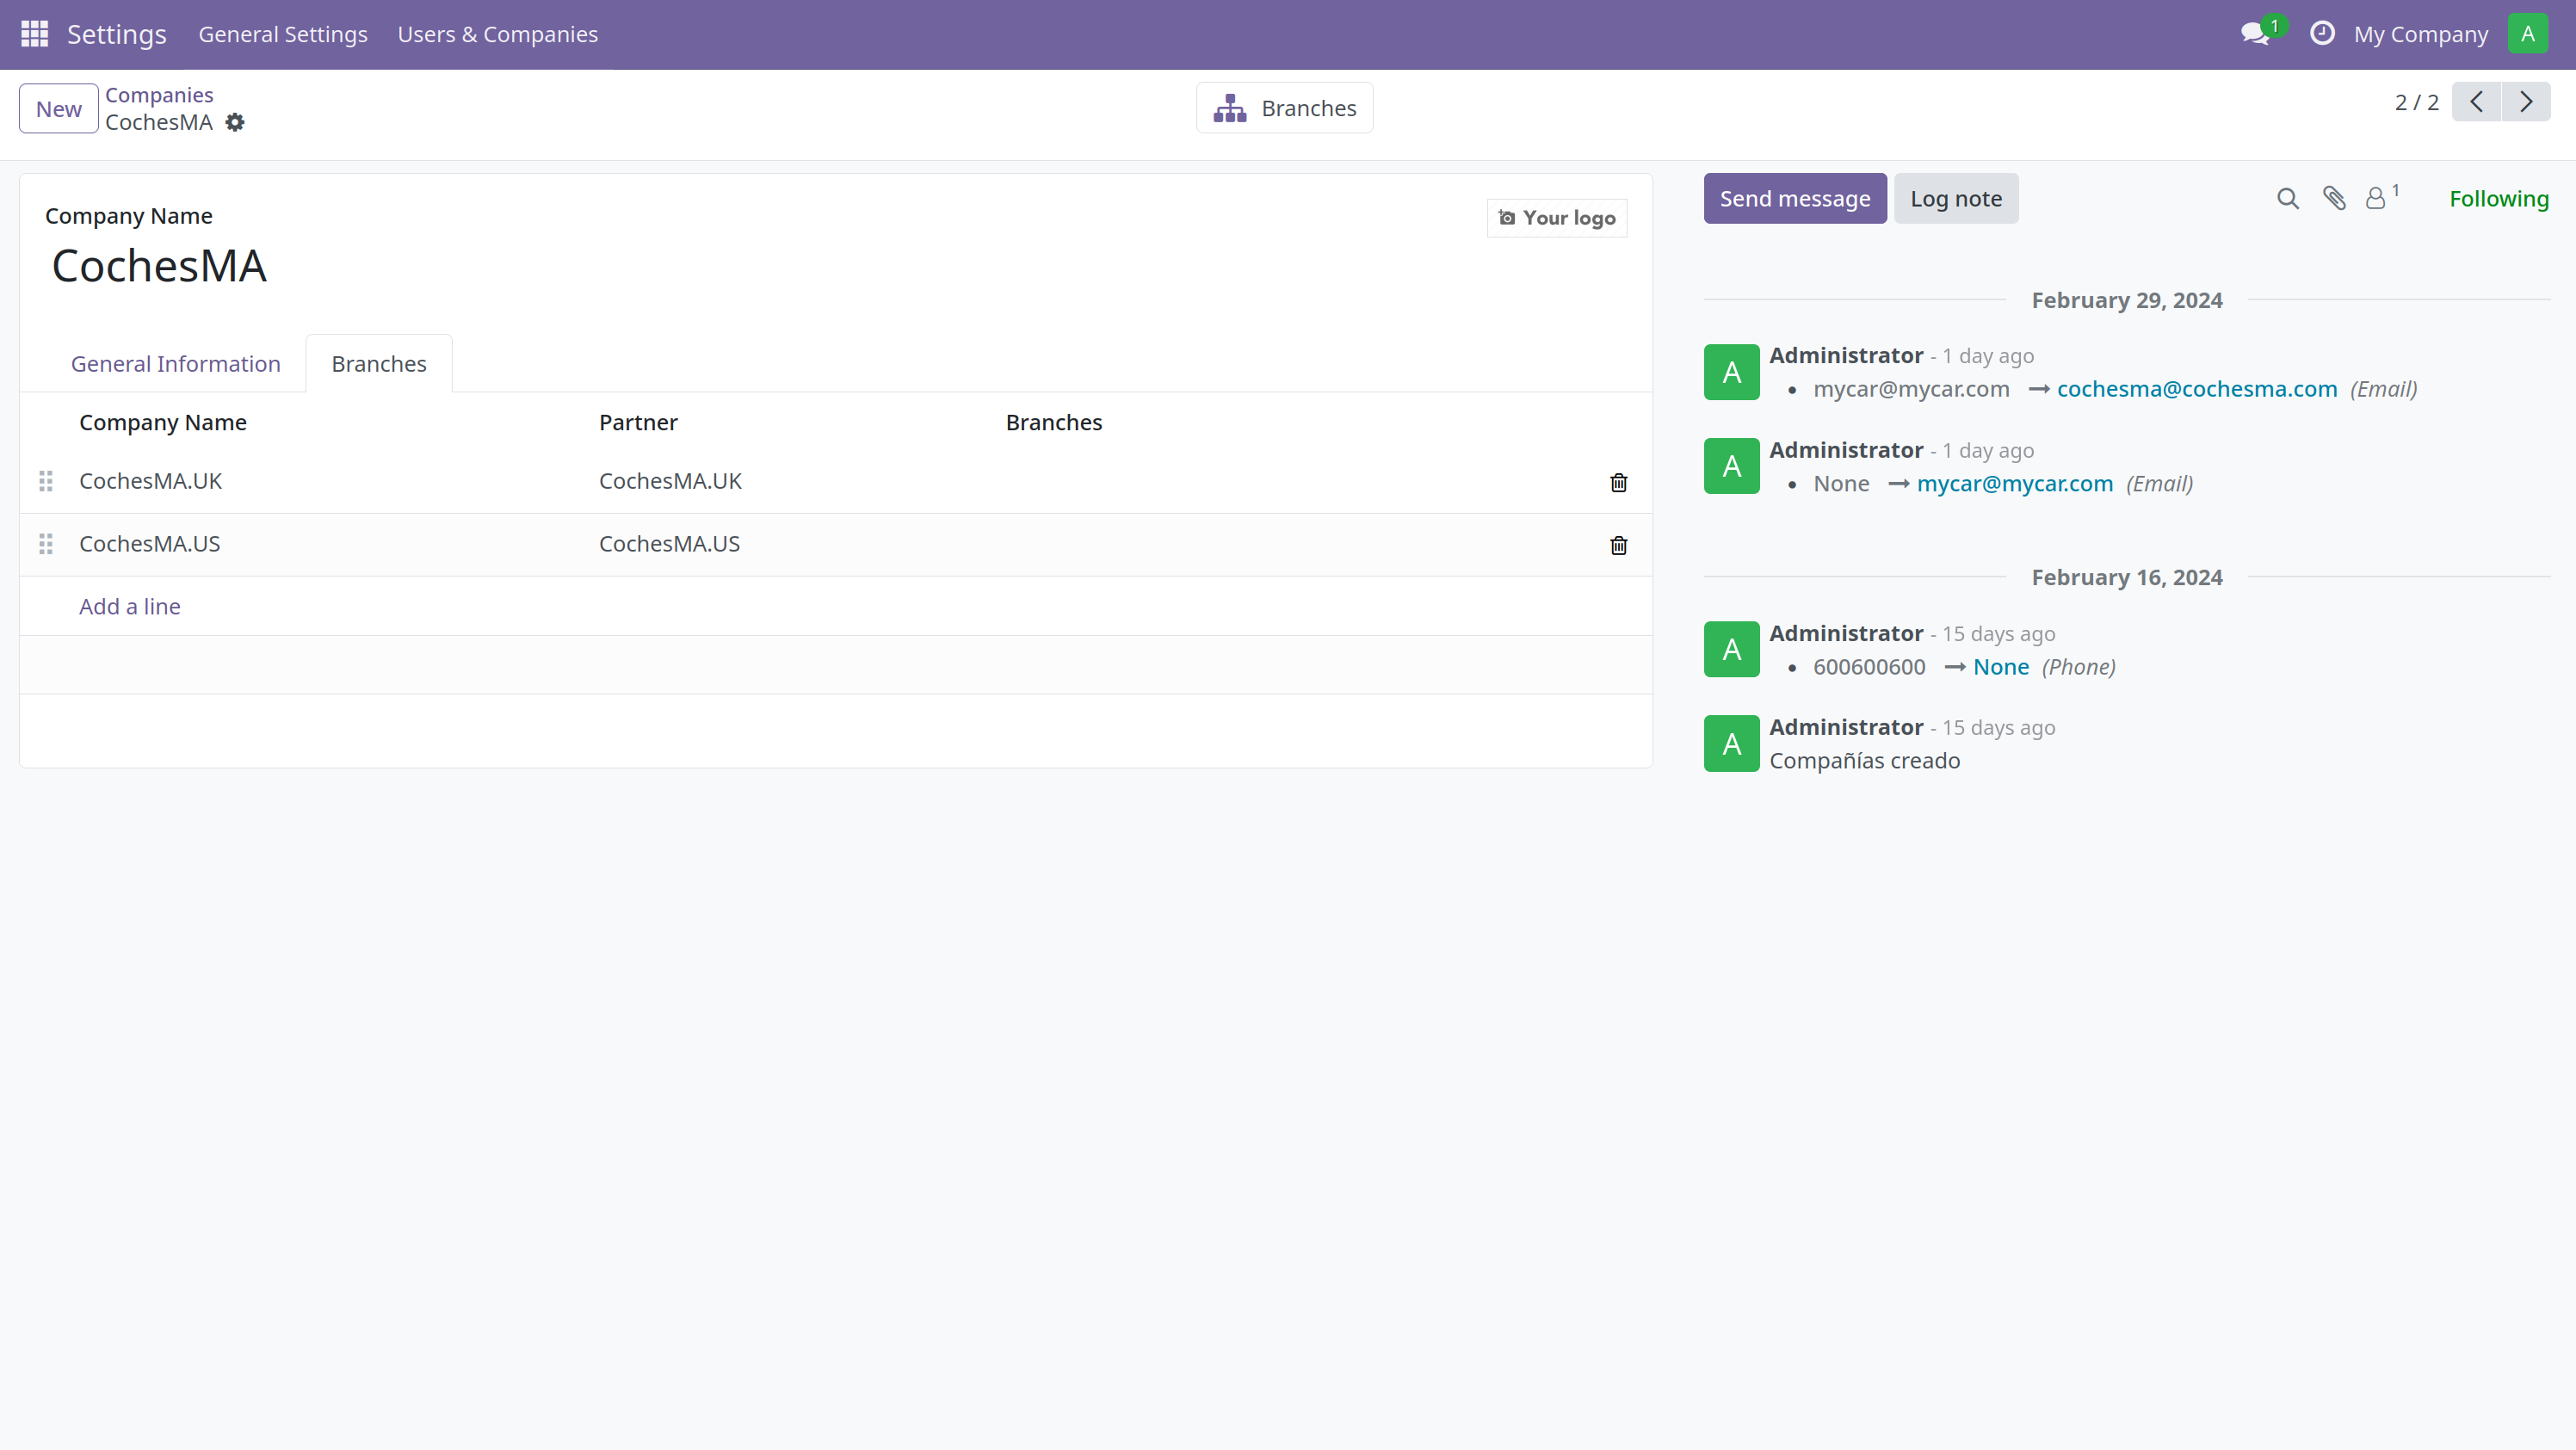
\includegraphics[width=6cm]{ramasCreadas.png}
    \caption{Página de administración de compañías rama con las compañías creadas.}
    \label{fig:faqs}
\end{figure}
\paragraph{}
A continuación, se va a explicar como se pueden crear usuarios para las compañías, tanto la matríz como las ramas. Como aparece en la figura 10, pulsa en el link Administrar usuarios y pulsa en New de la esquina superior izquierda. 
\begin{figure}[h]
    \centering
    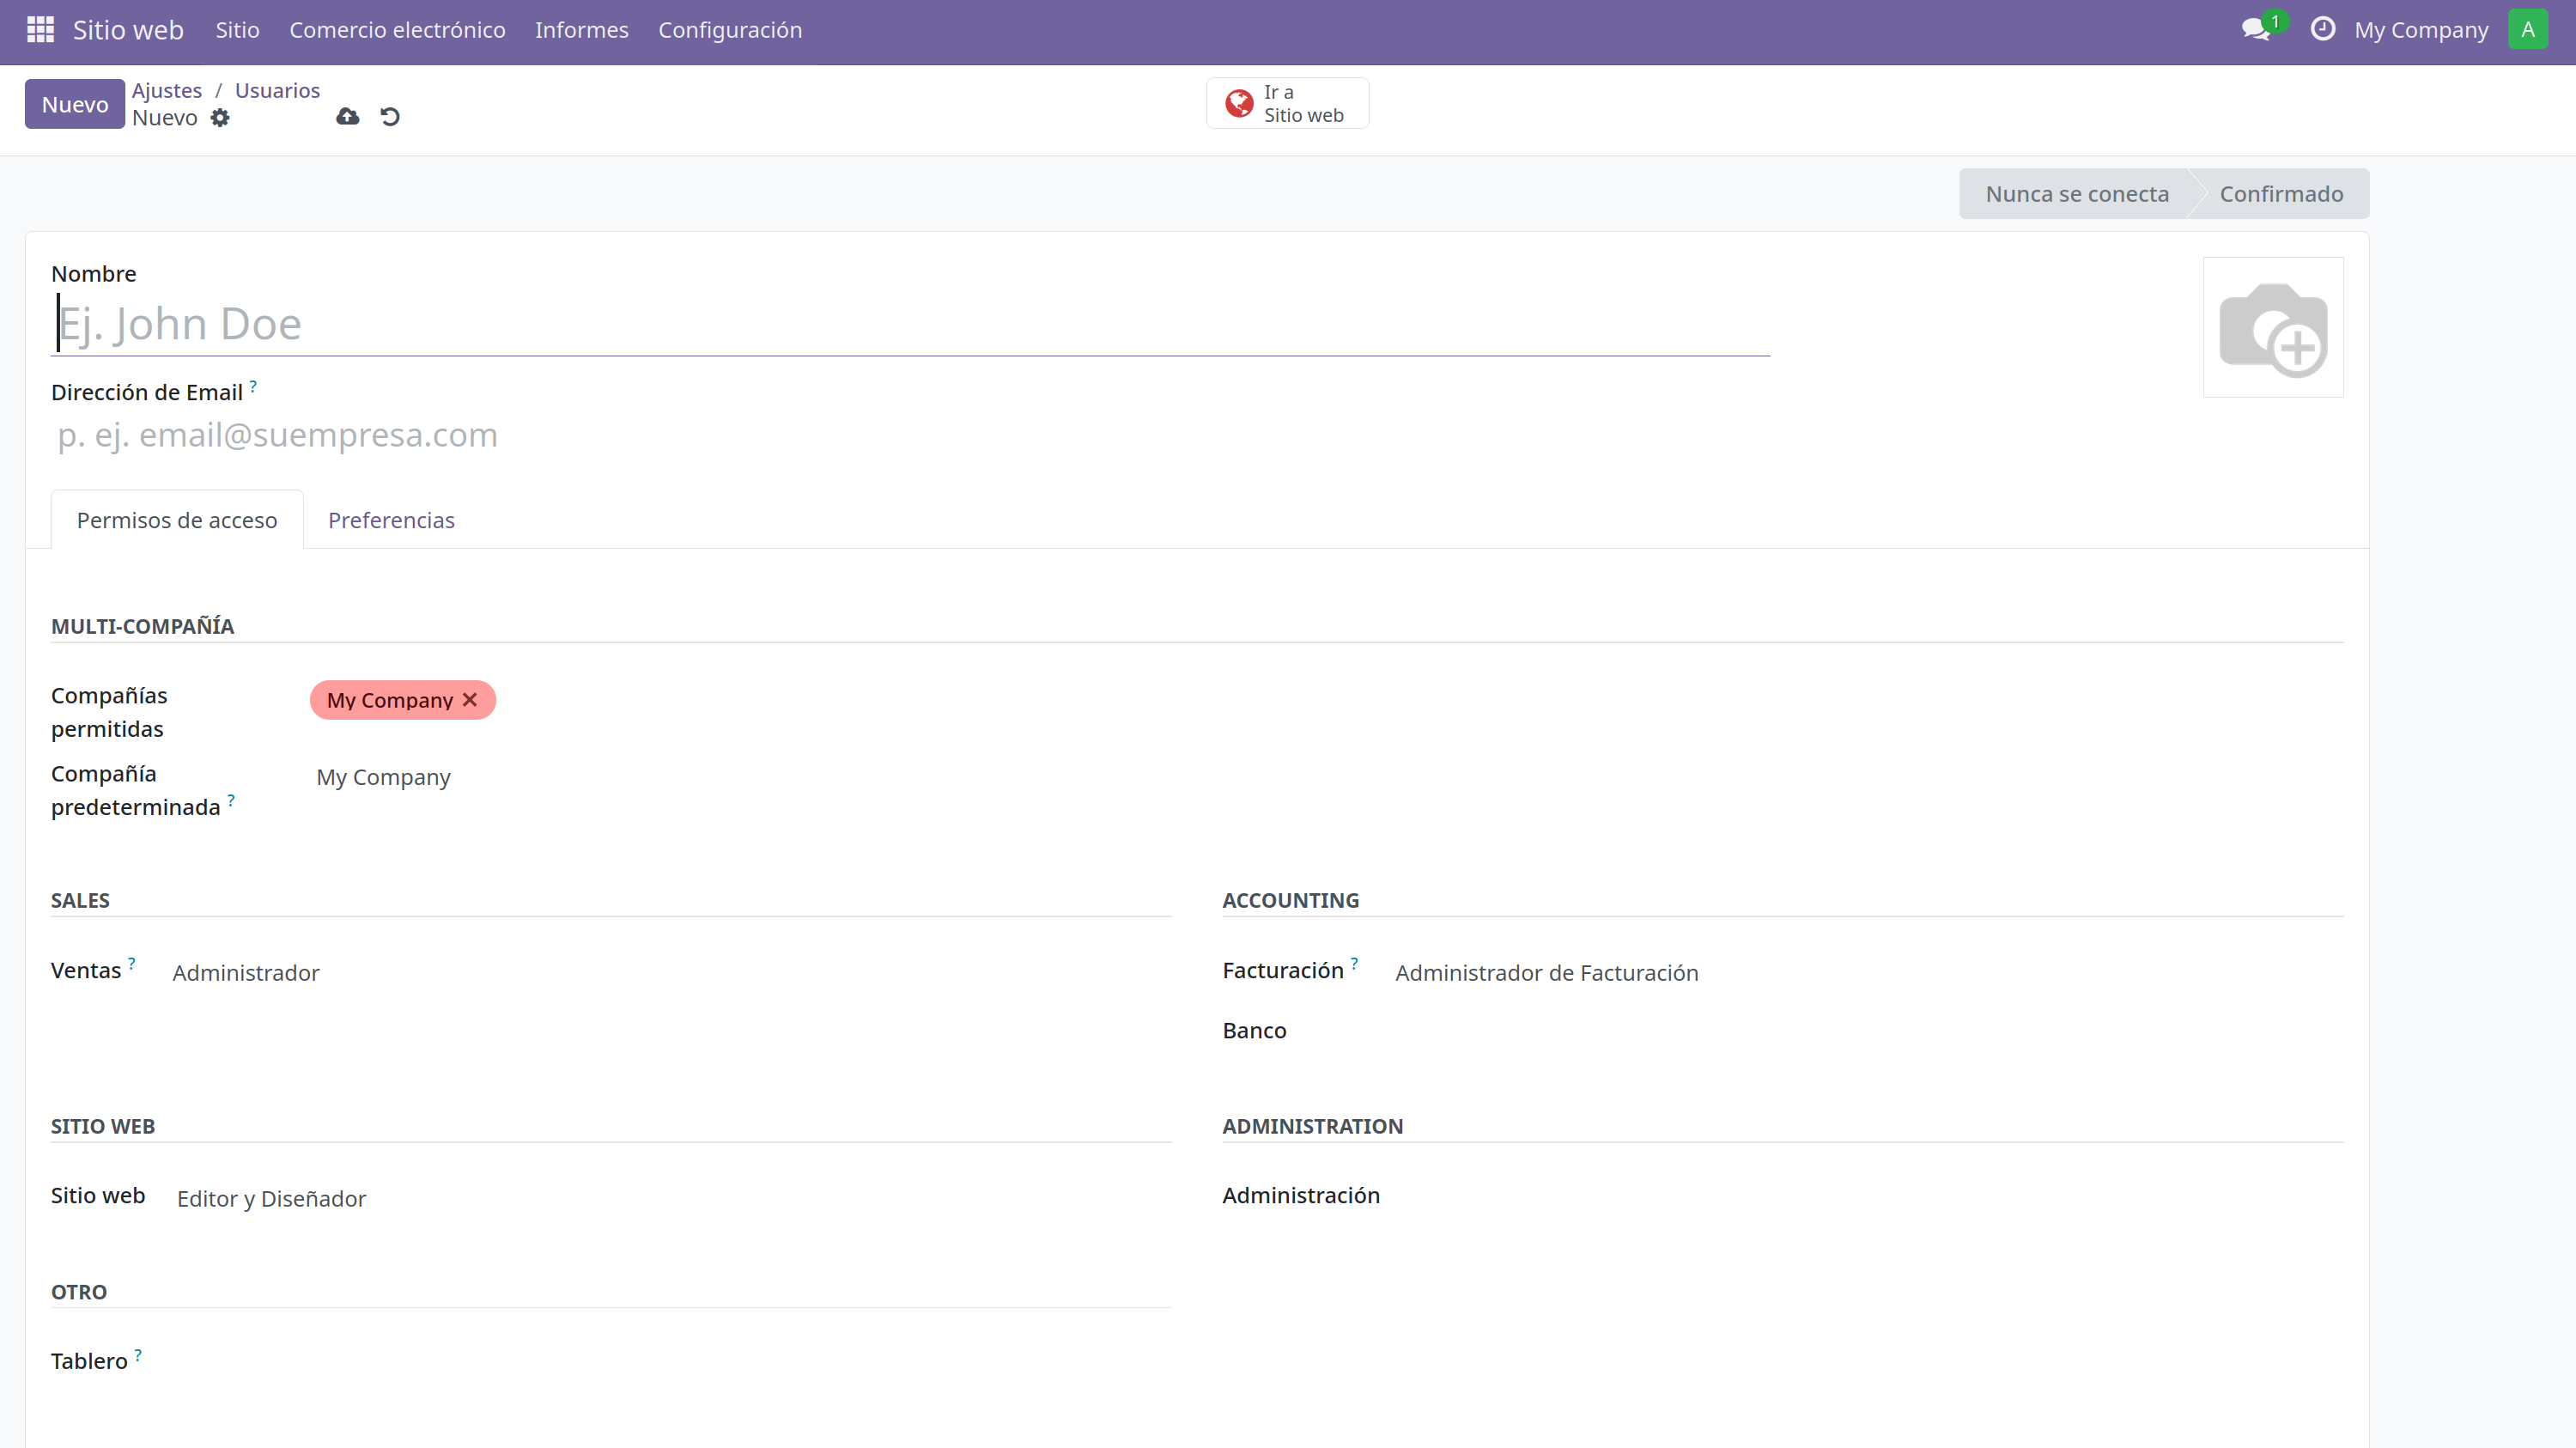
\includegraphics[width=6cm]{adminUsuarios.png}
    \caption{Página de creación de usuario de la compañía.}
    \label{fig:faqs}
\end{figure}
\paragraph{}
Introduce la información correspondiente al usuario que se quiere crear, también se puede elegir que compañías tiene acceso cada usuario si se hace click en Compañias predeterminadas y Compañía predeterminada y escogiendo la compañía deseada. Una vez realizado pulsa en Save and Close. Si se navega hacia atrás a la página de administración de usuarios se verá que se ha creado un nuevo usuario.
Si se quiere cambiar el idioma de la compañía, se debe ir al menú de preferencias y seleccionar el idioma deseado en la opción de Languagues.
\newpage
\begin{figure}[h]
    \centering
    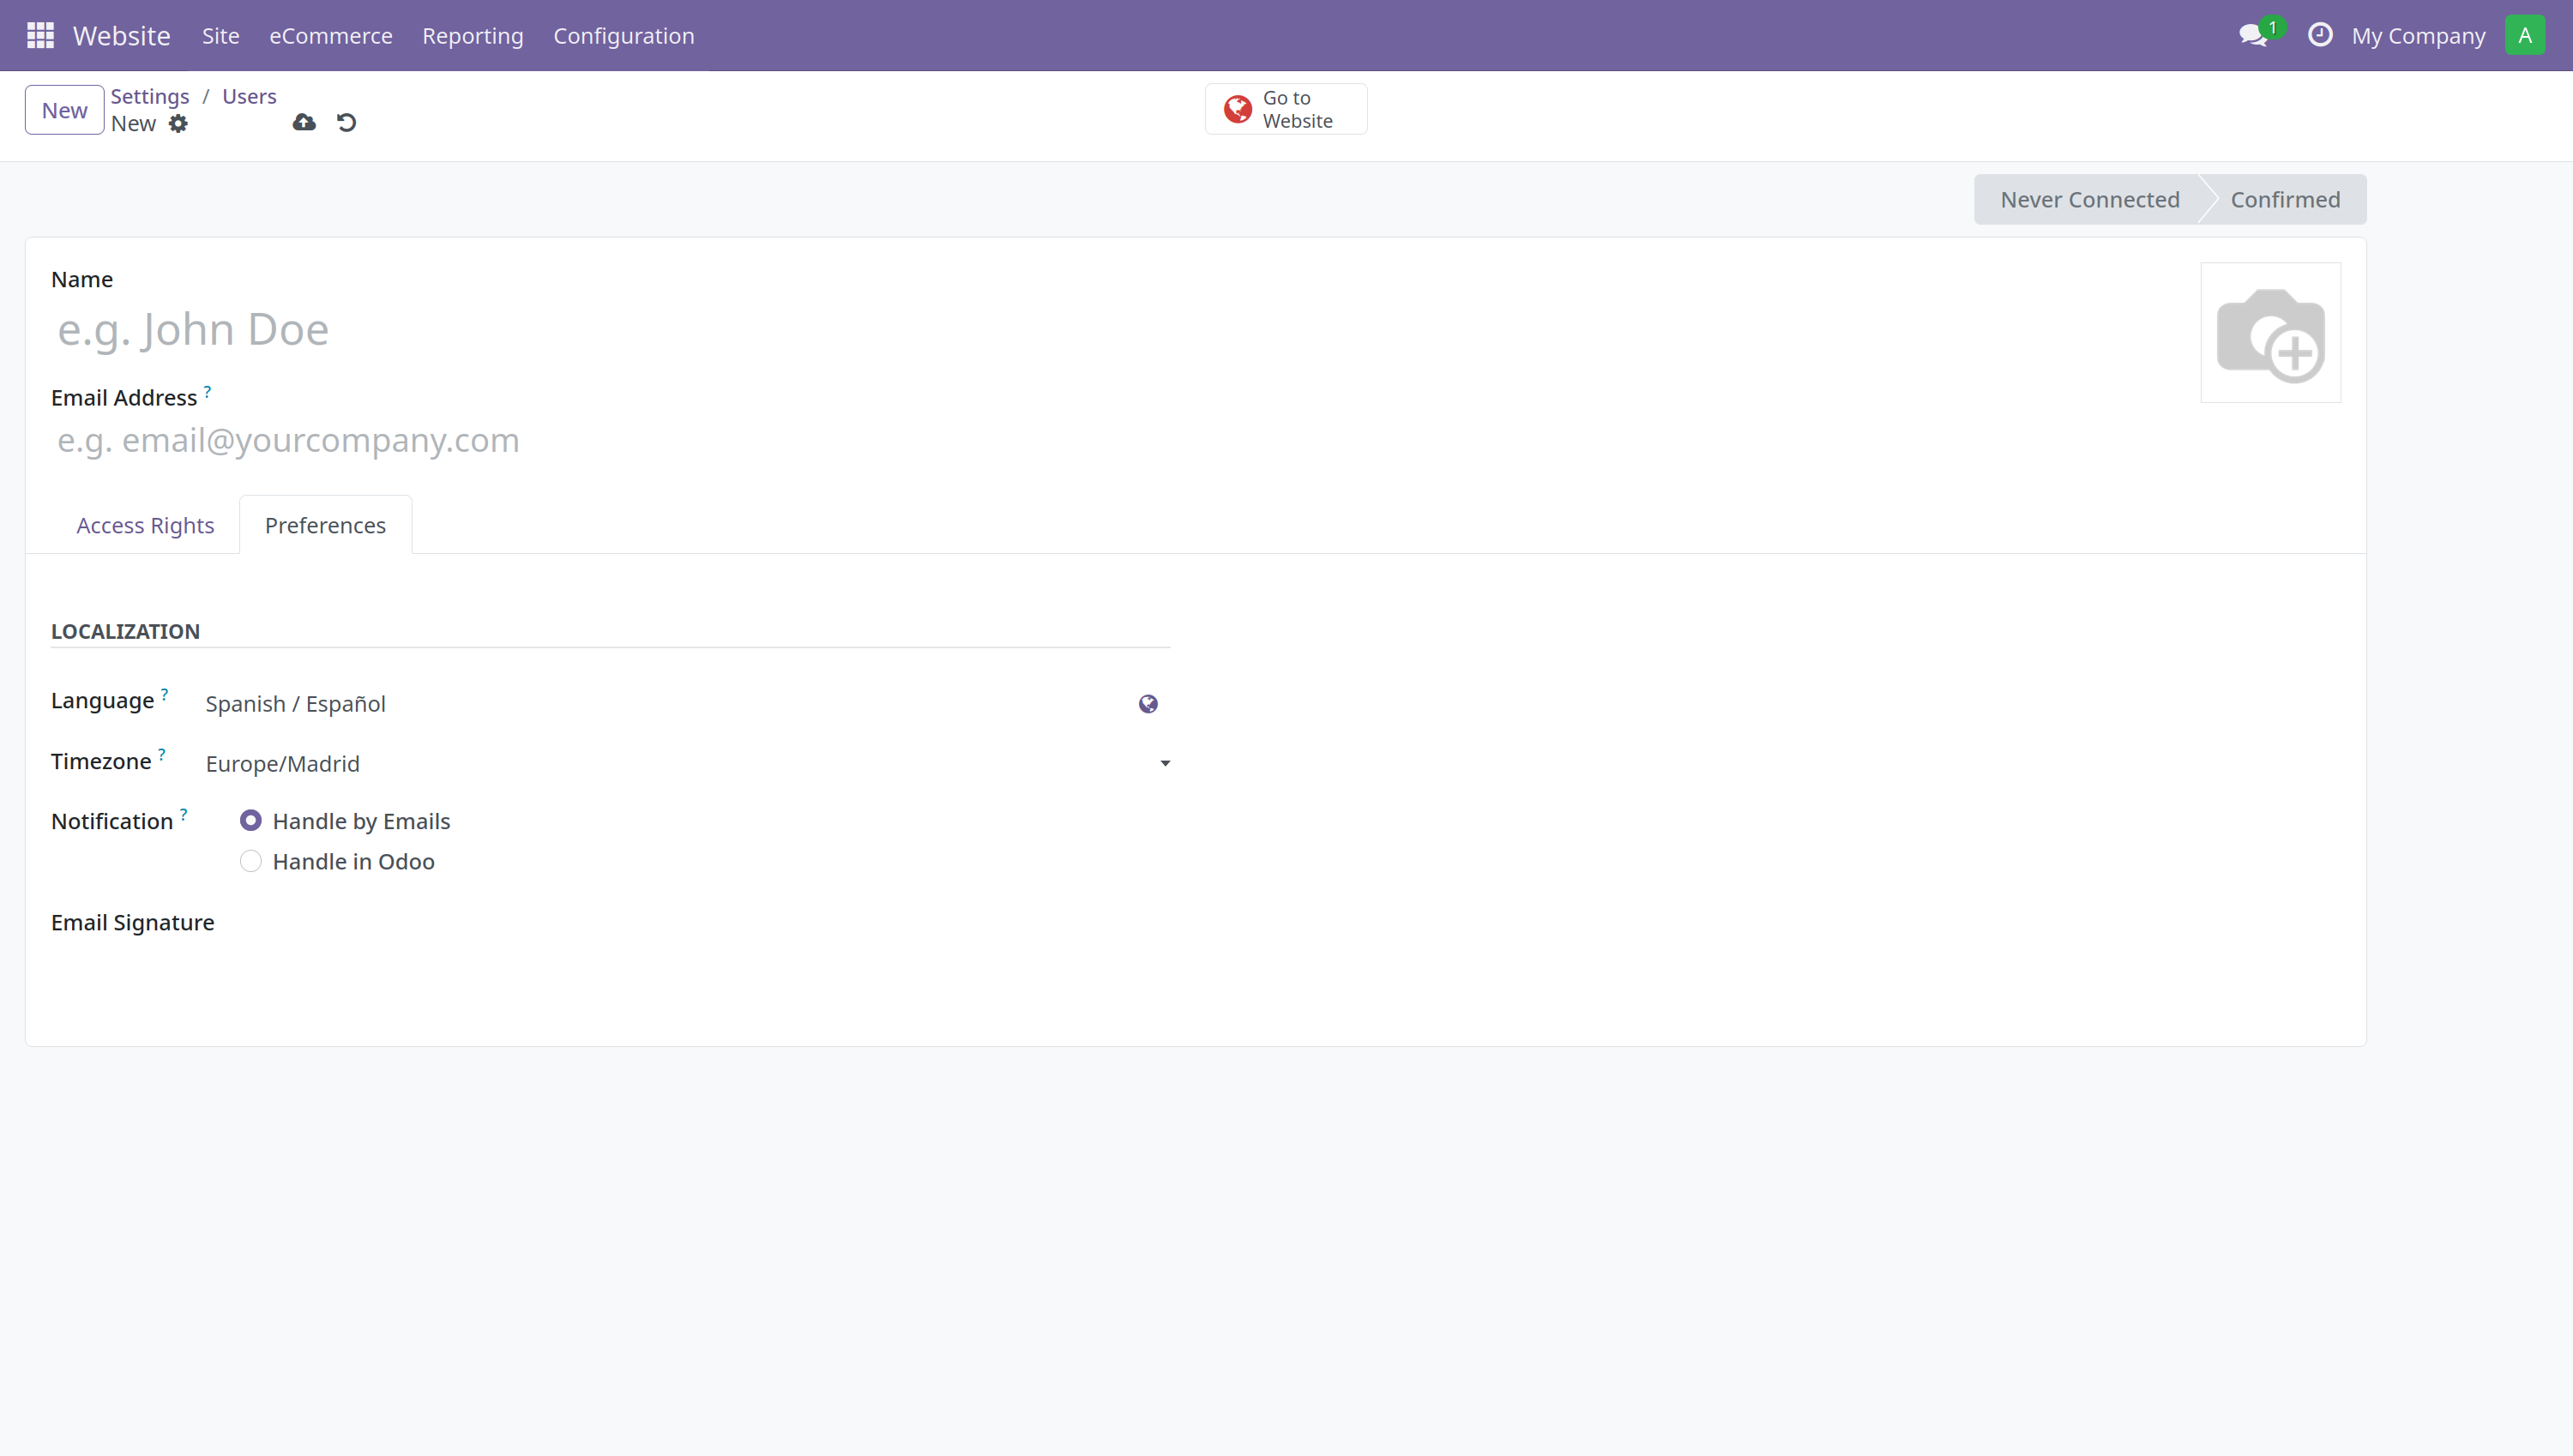
\includegraphics[width=6cm]{languageUsuario.png}
    \caption{Página de preferencias del usuario.}
    \label{fig:faqs}
\end{figure}
\paragraph{}
Se puede añadir idiomas si no se encuentran en la lista de idiomas disponibles. Para ello, se debe hacer click en el icono del mundo de la opción de Languagues y seleccionar el idioma deseado.
\begin{figure}[h]
    \centering
    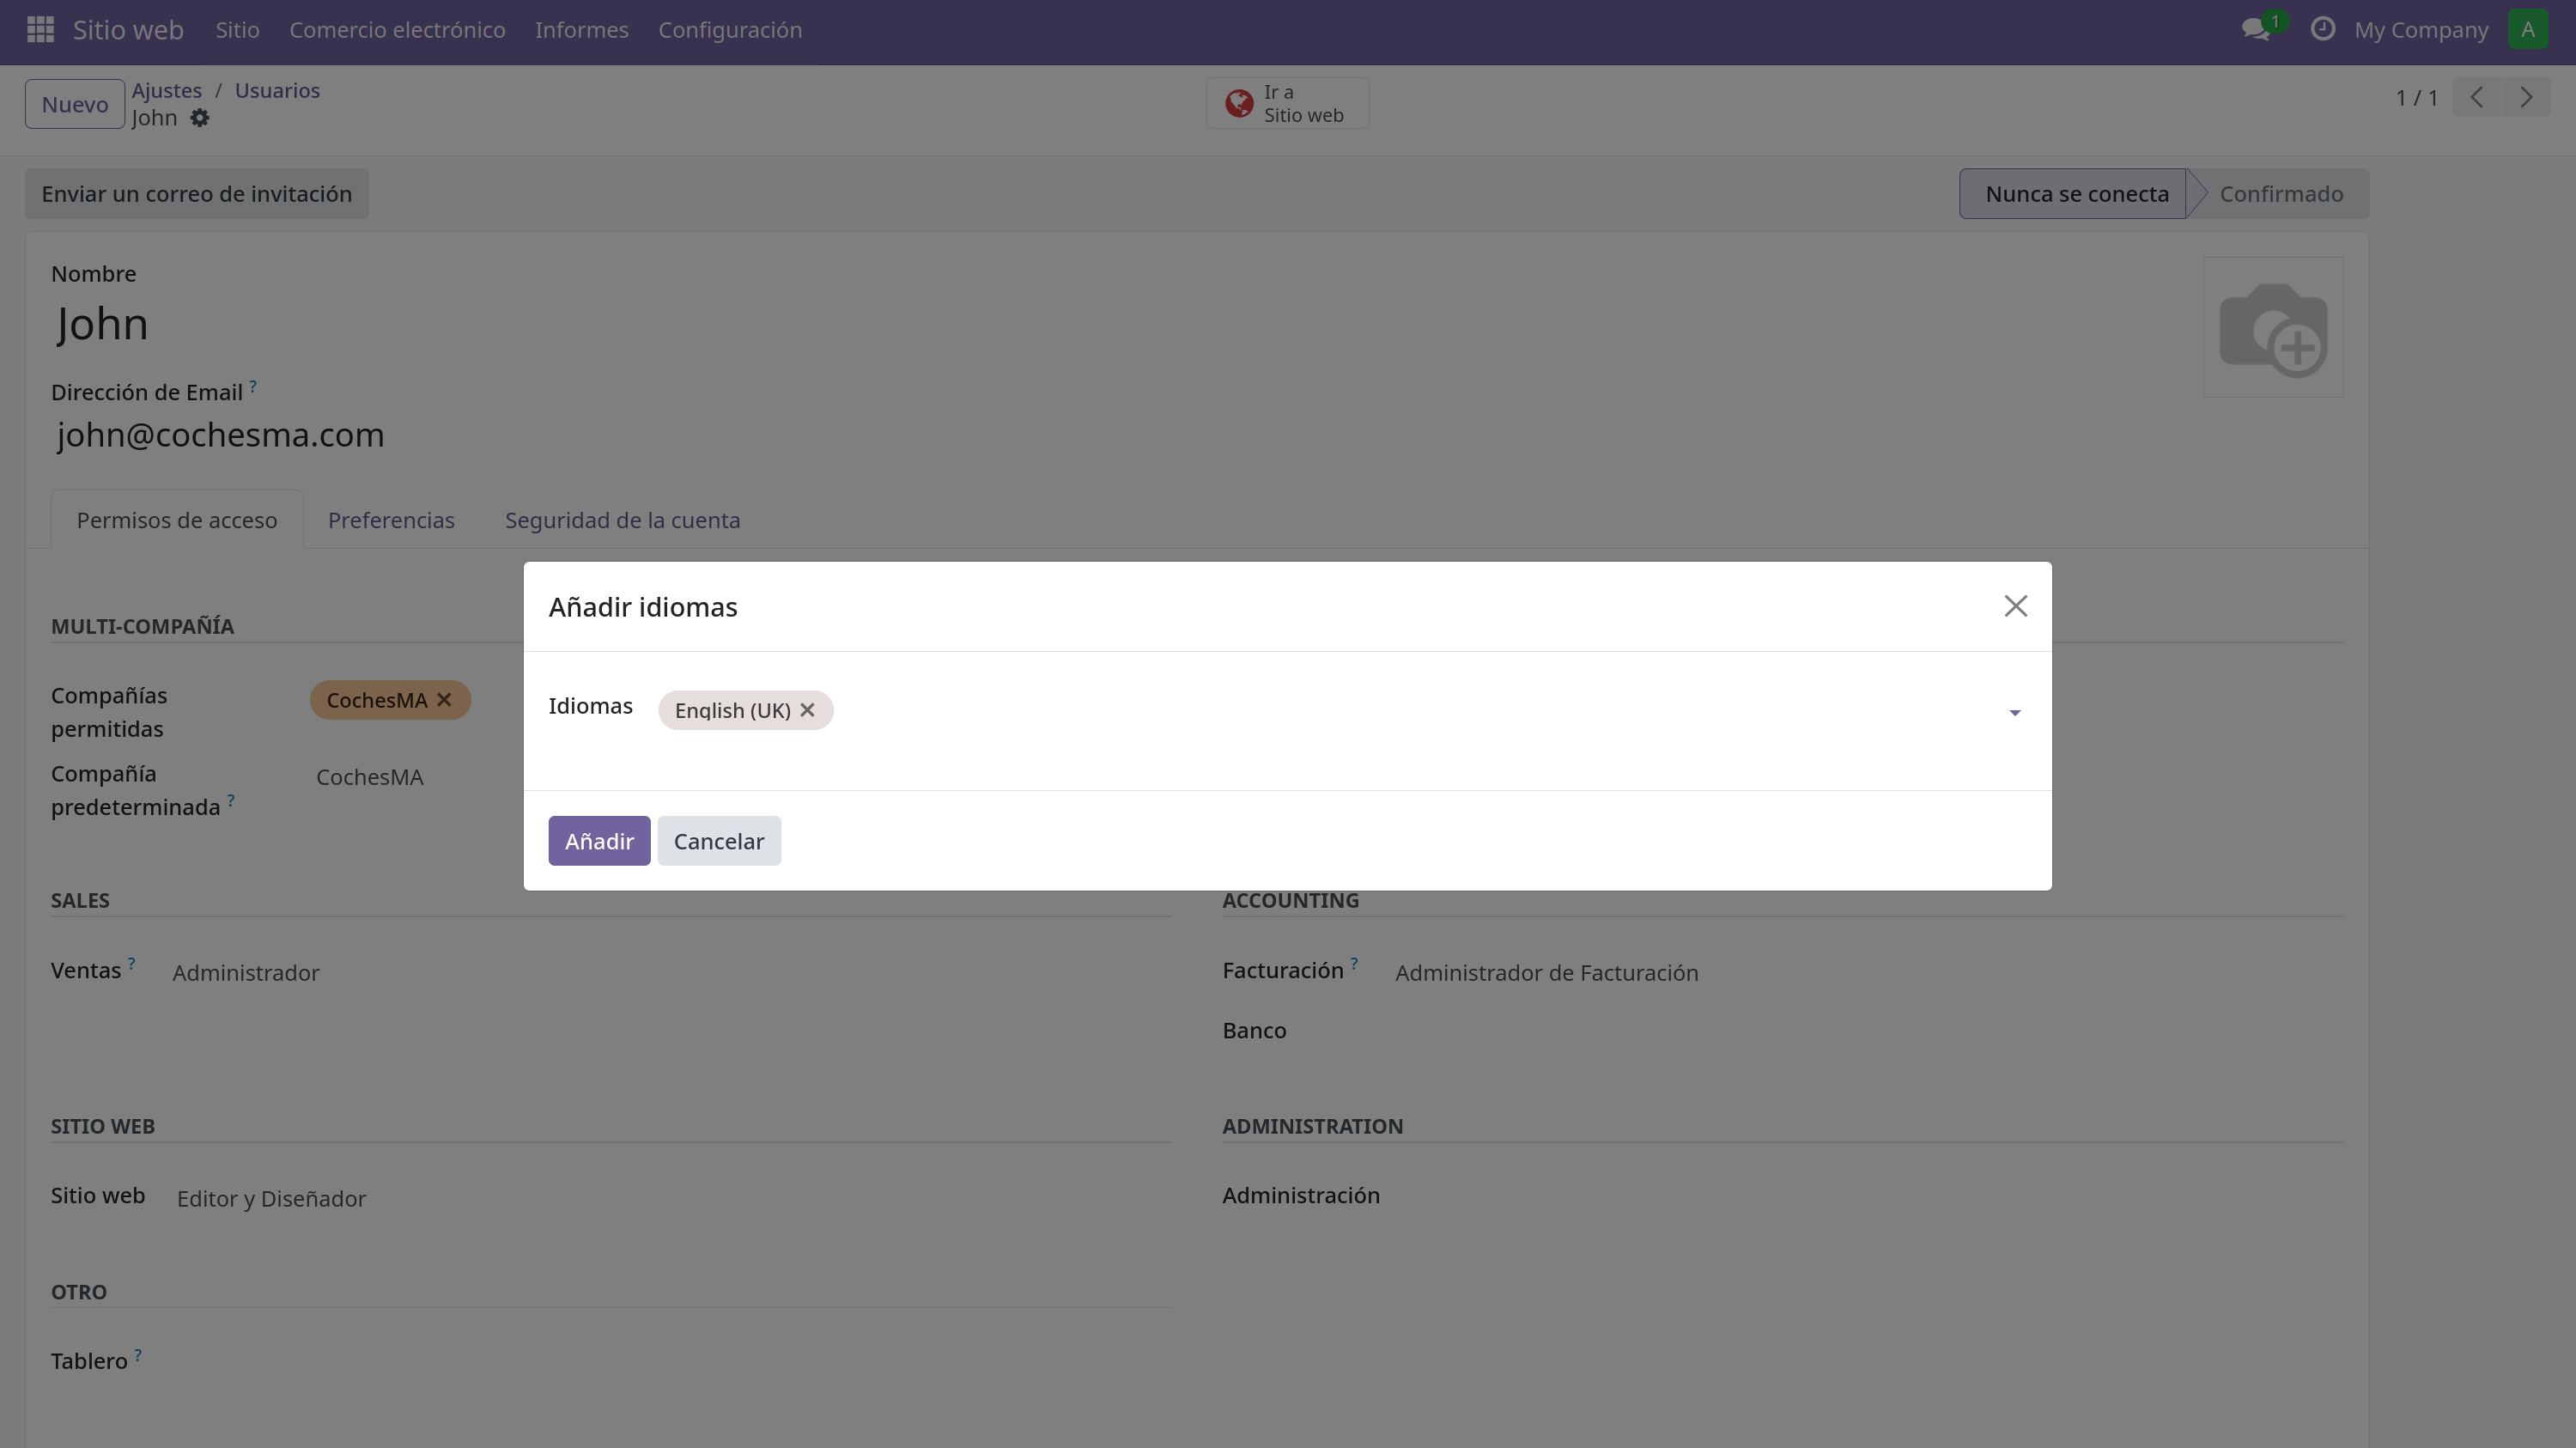
\includegraphics[width=6cm]{añadirIdioma.png}
    \caption{Menú de añadir un idioma.}
    \label{fig:faqs}
\end{figure}
\paragraph{}
Repite este proceso tantas veces como usuarios se quiere crear.
\begin{figure}[h]
    \centering
    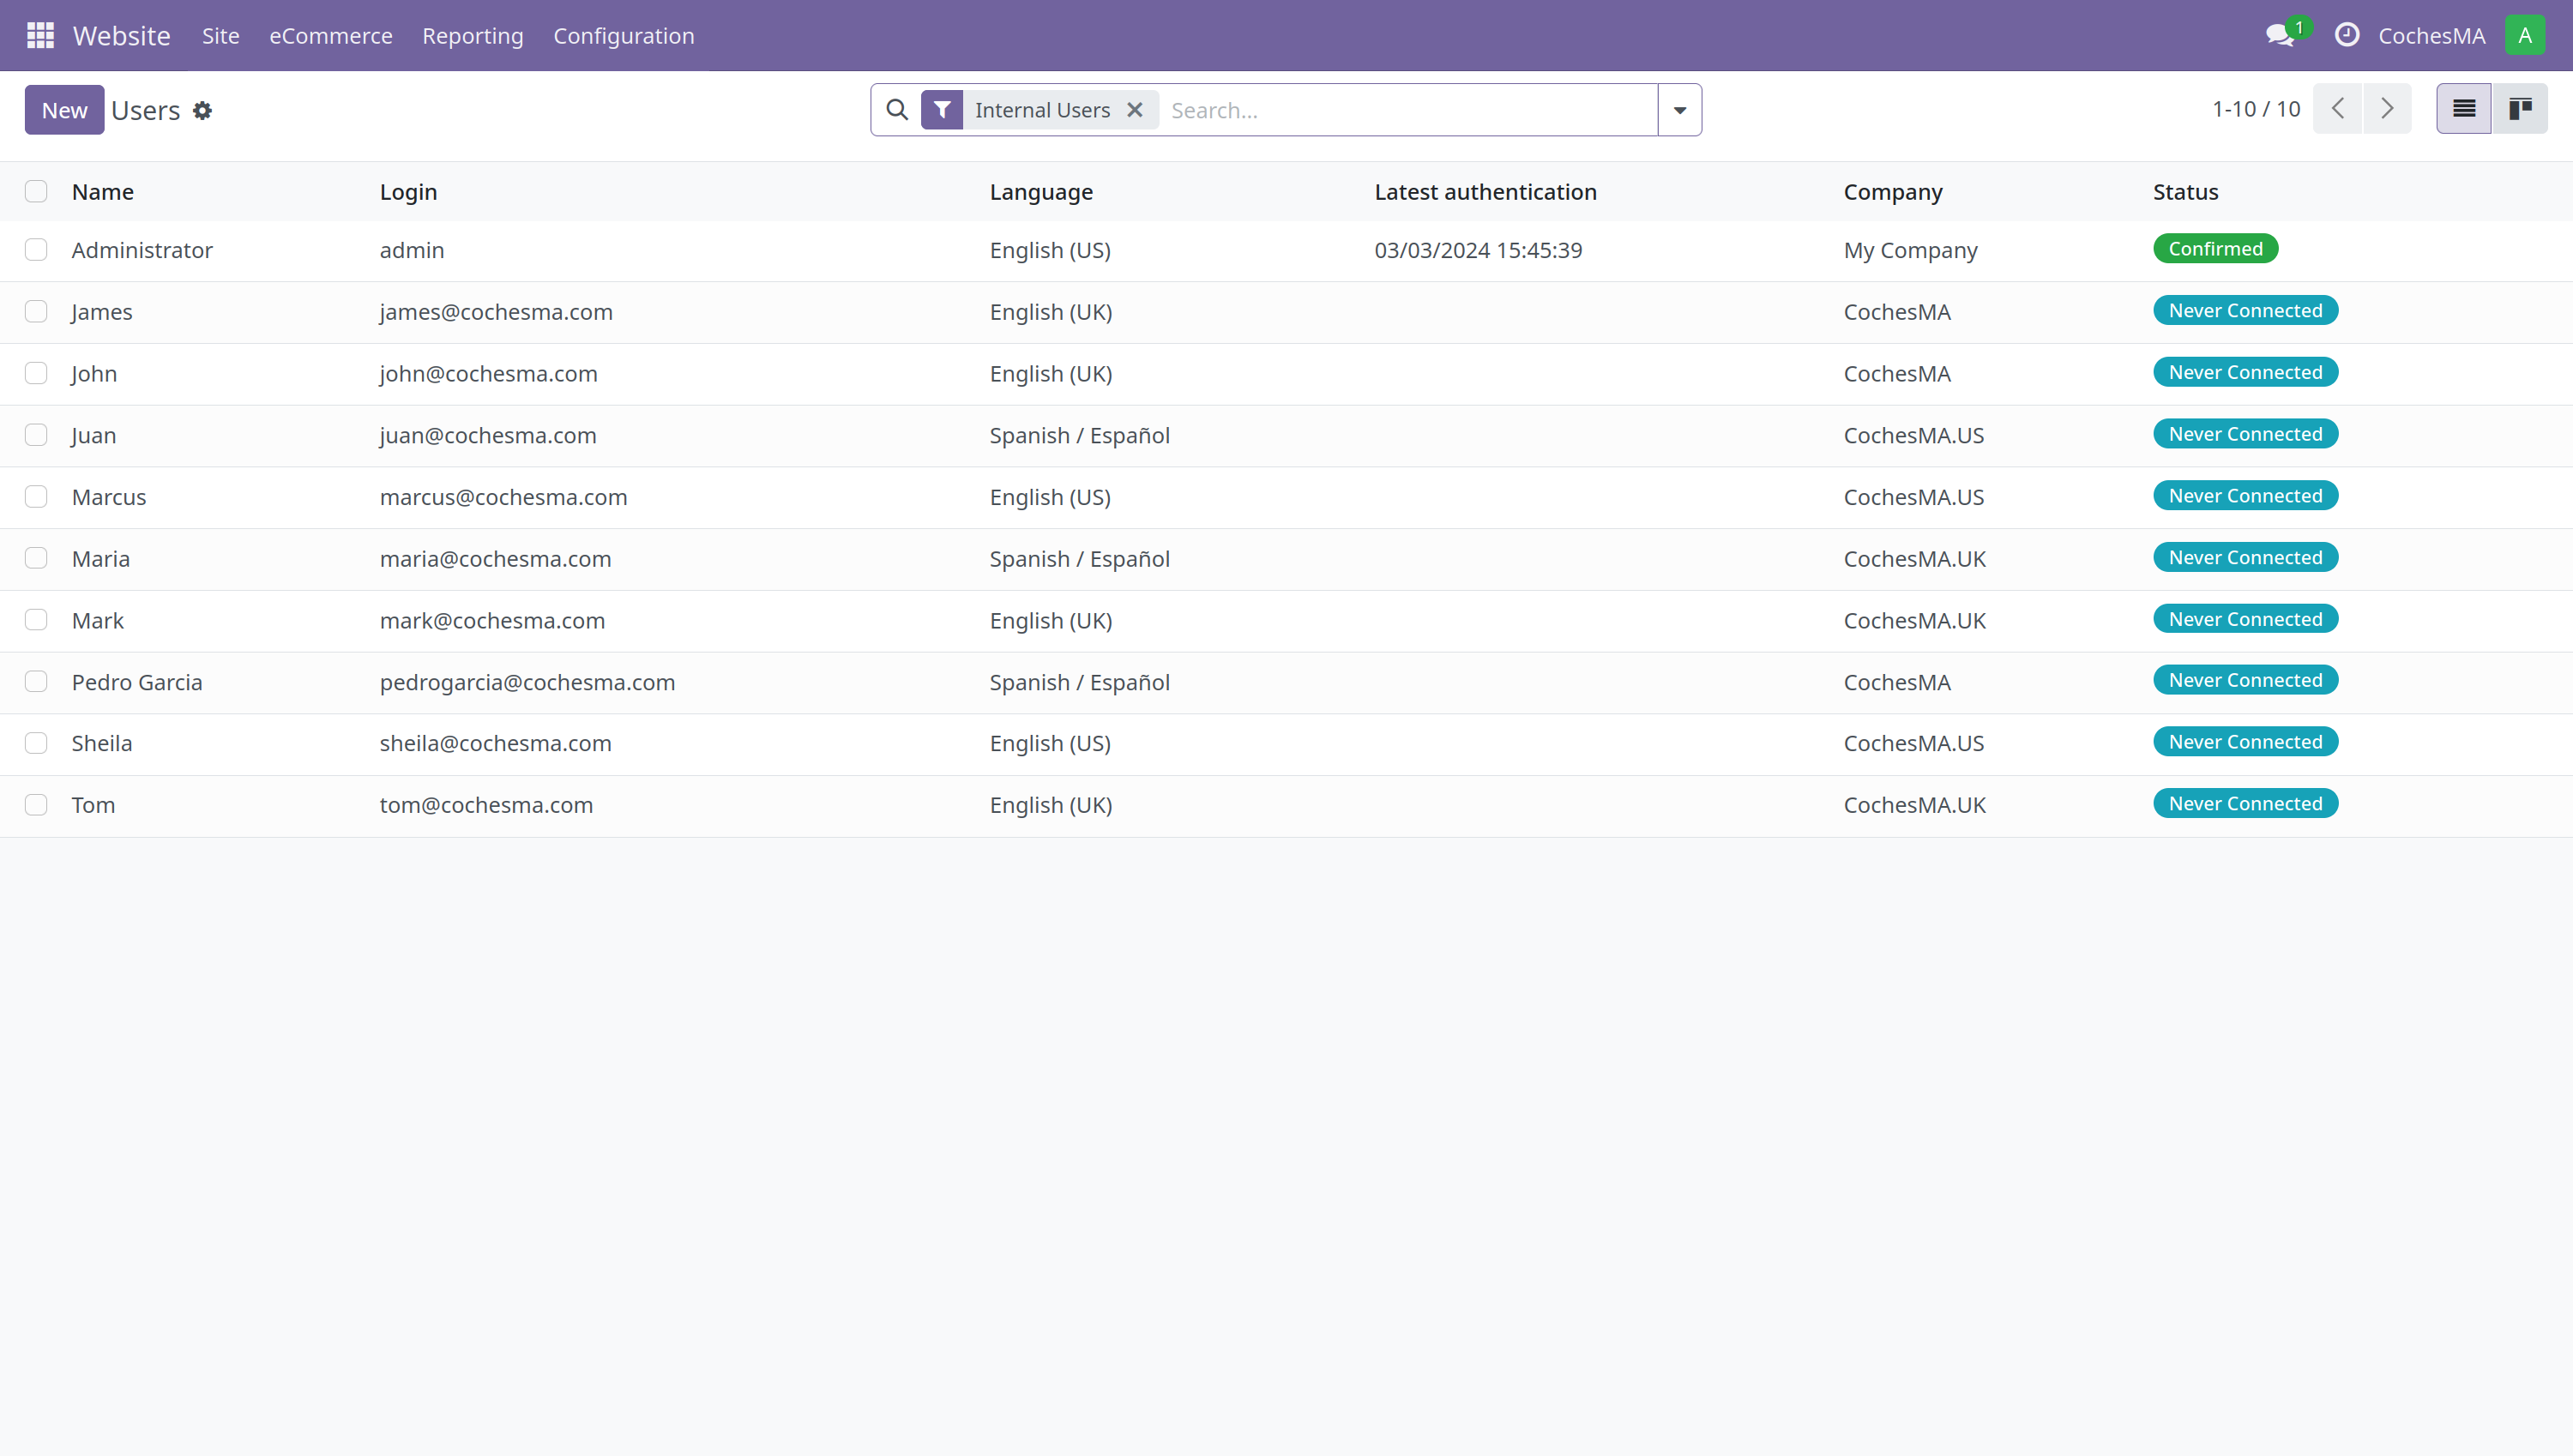
\includegraphics[width=6cm]{usuarios.png}
    \caption{Página de usuarios de la compañía.}
    \label{fig:faqs}
\end{figure}
\paragraph{}
Una vez añadido usuarios con sus respectivos idiomas, se puede añadir un nuevo idioma a la compañía. Para ello, se debe ir al menú de configuración de la web y selecciona el idioma que se quiere añadir dentro del menú de Información de la web.
\newpage
\begin{figure}[h]
    \centering
    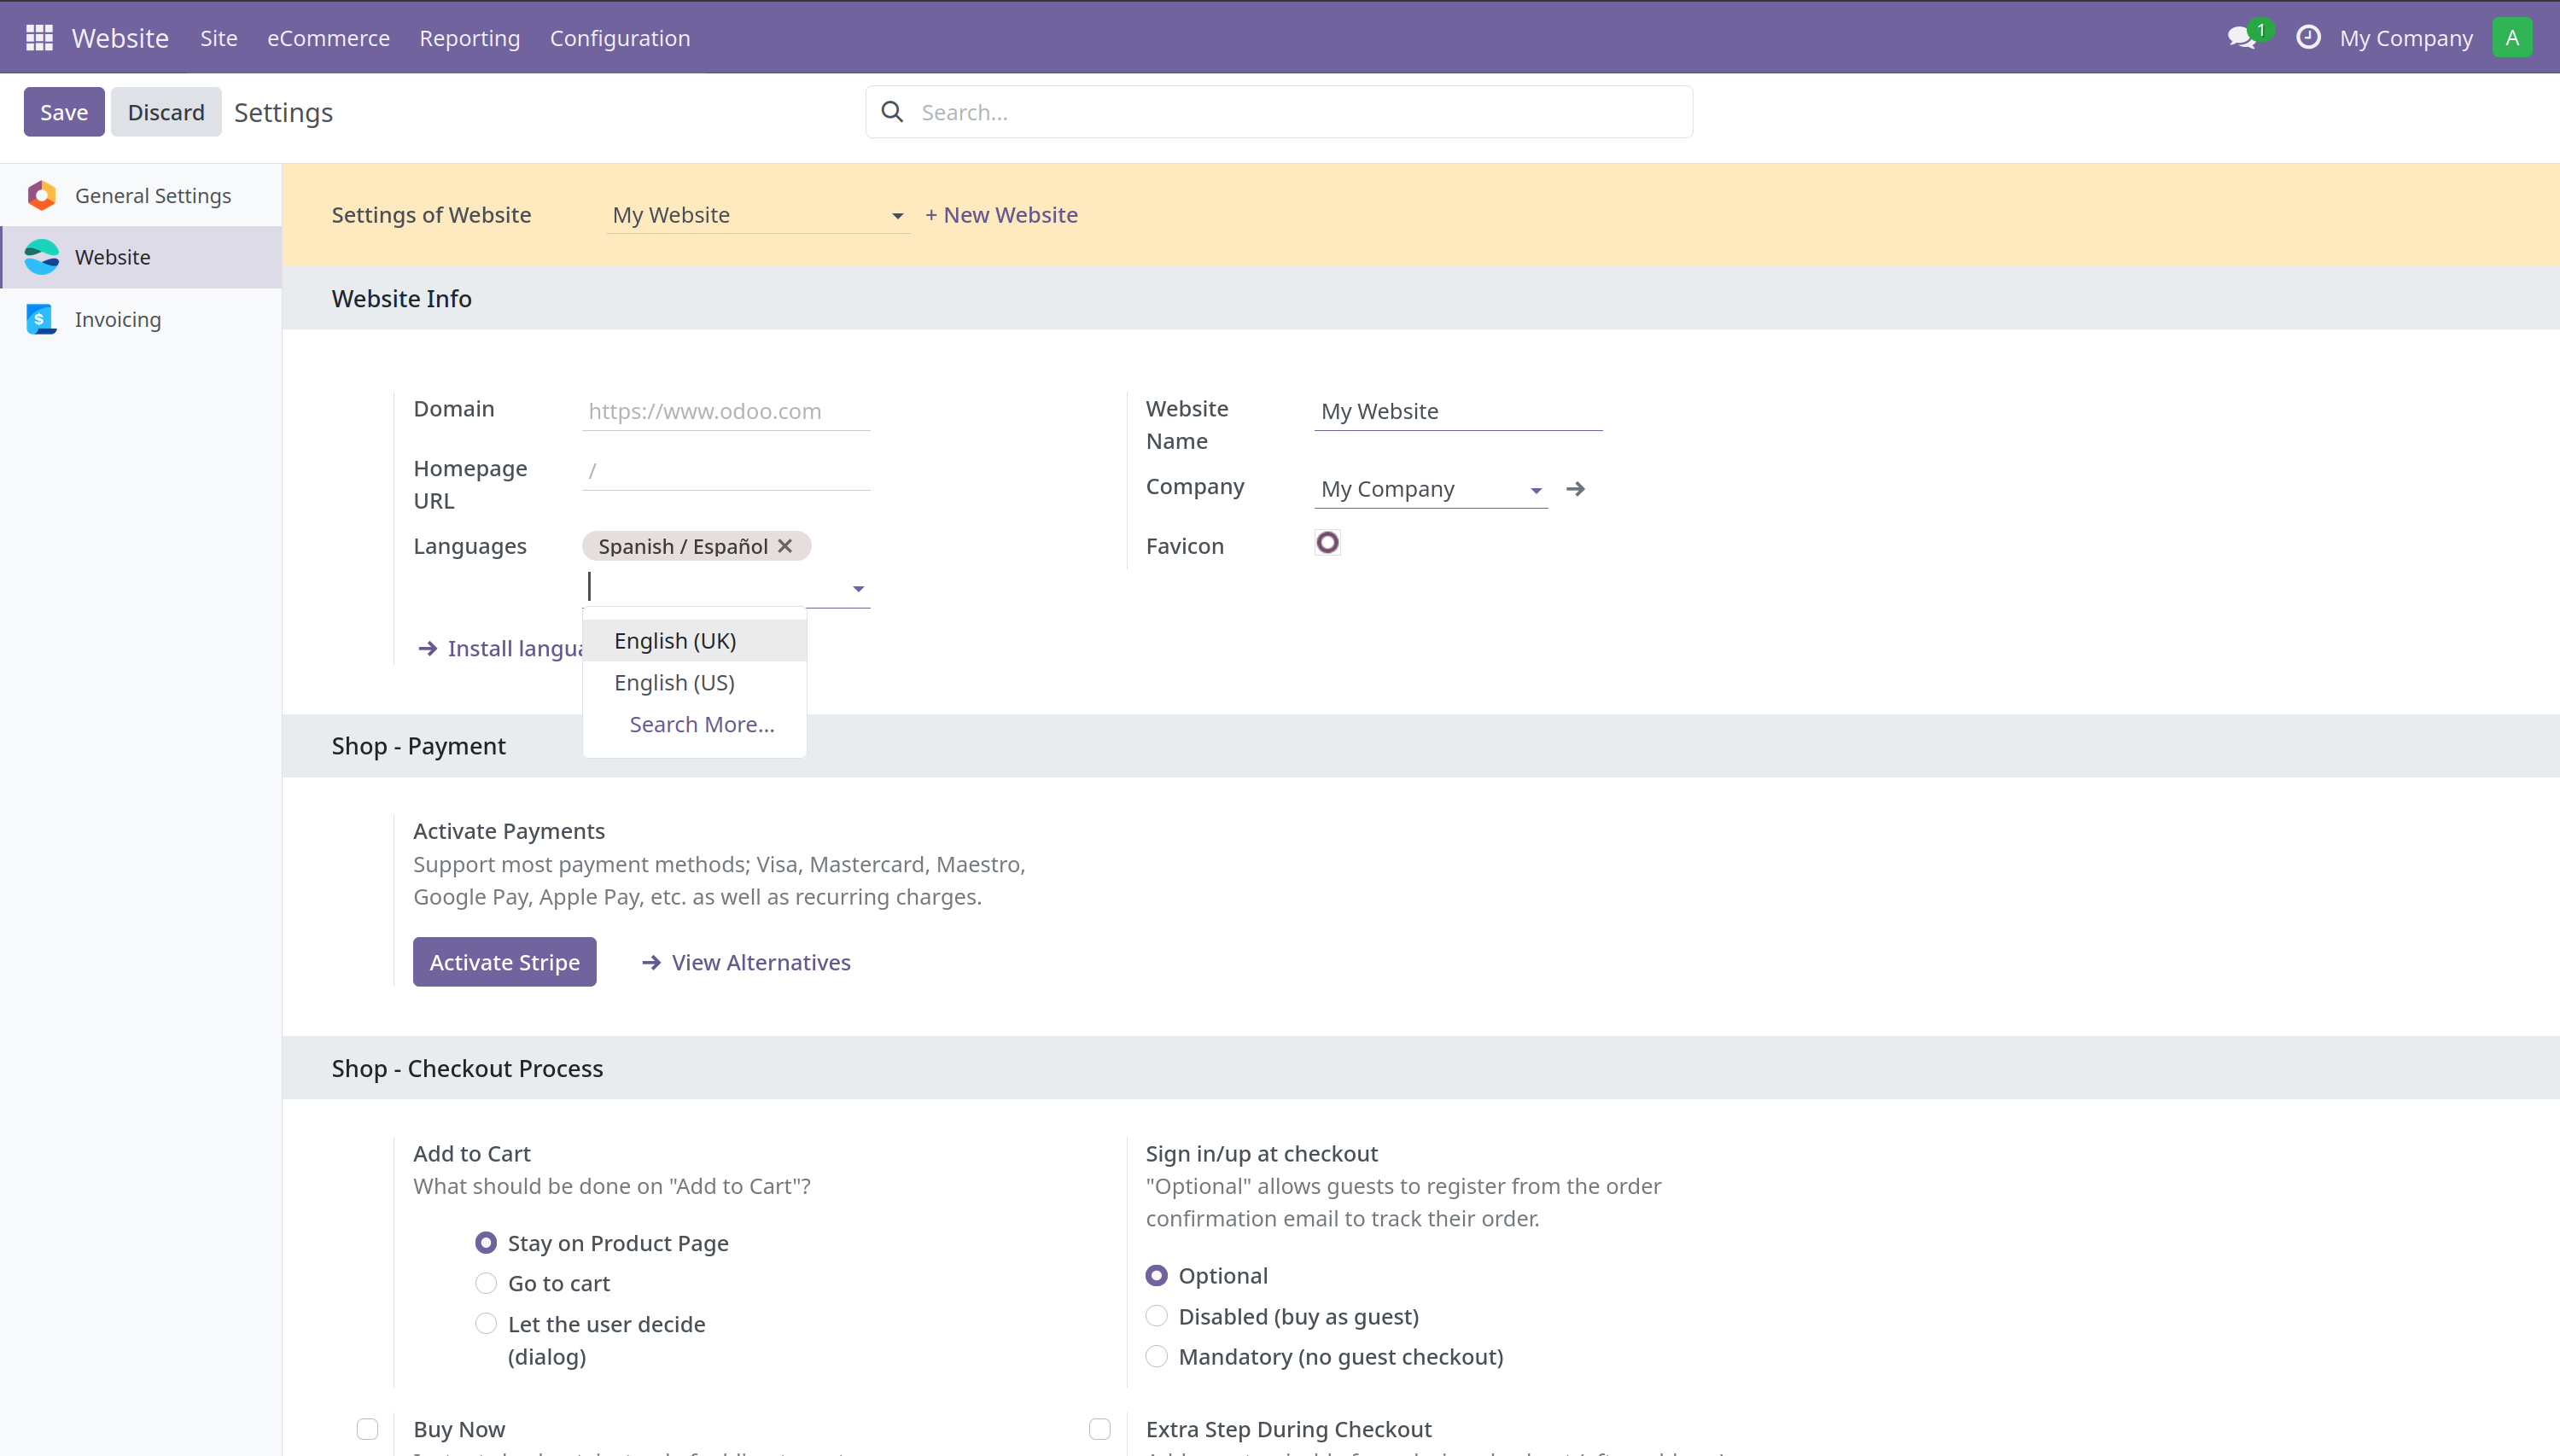
\includegraphics[width=6cm]{añadirIdiomaWeb.png}
    \caption{Página para añadir idioma a la web.}
    \label{fig:faqs}
\end{figure}
\paragraph{}
Además, se pueden añadir distintas funcionalidades de internalización a la web a parte del idioma que se ha explicado anteriormente, como por ejemplo la moneda.
Para ello se debe ir al menú de administración de las compañías y selecionar la compañía matriz. Una vez dentro haz click en el desplegable de la opción Moneda y selecciona Buscar más. Activa las monedas que se quieren añadir en las compañías ramas de la siguiente manera.
\begin{figure}[h]
    \centering
    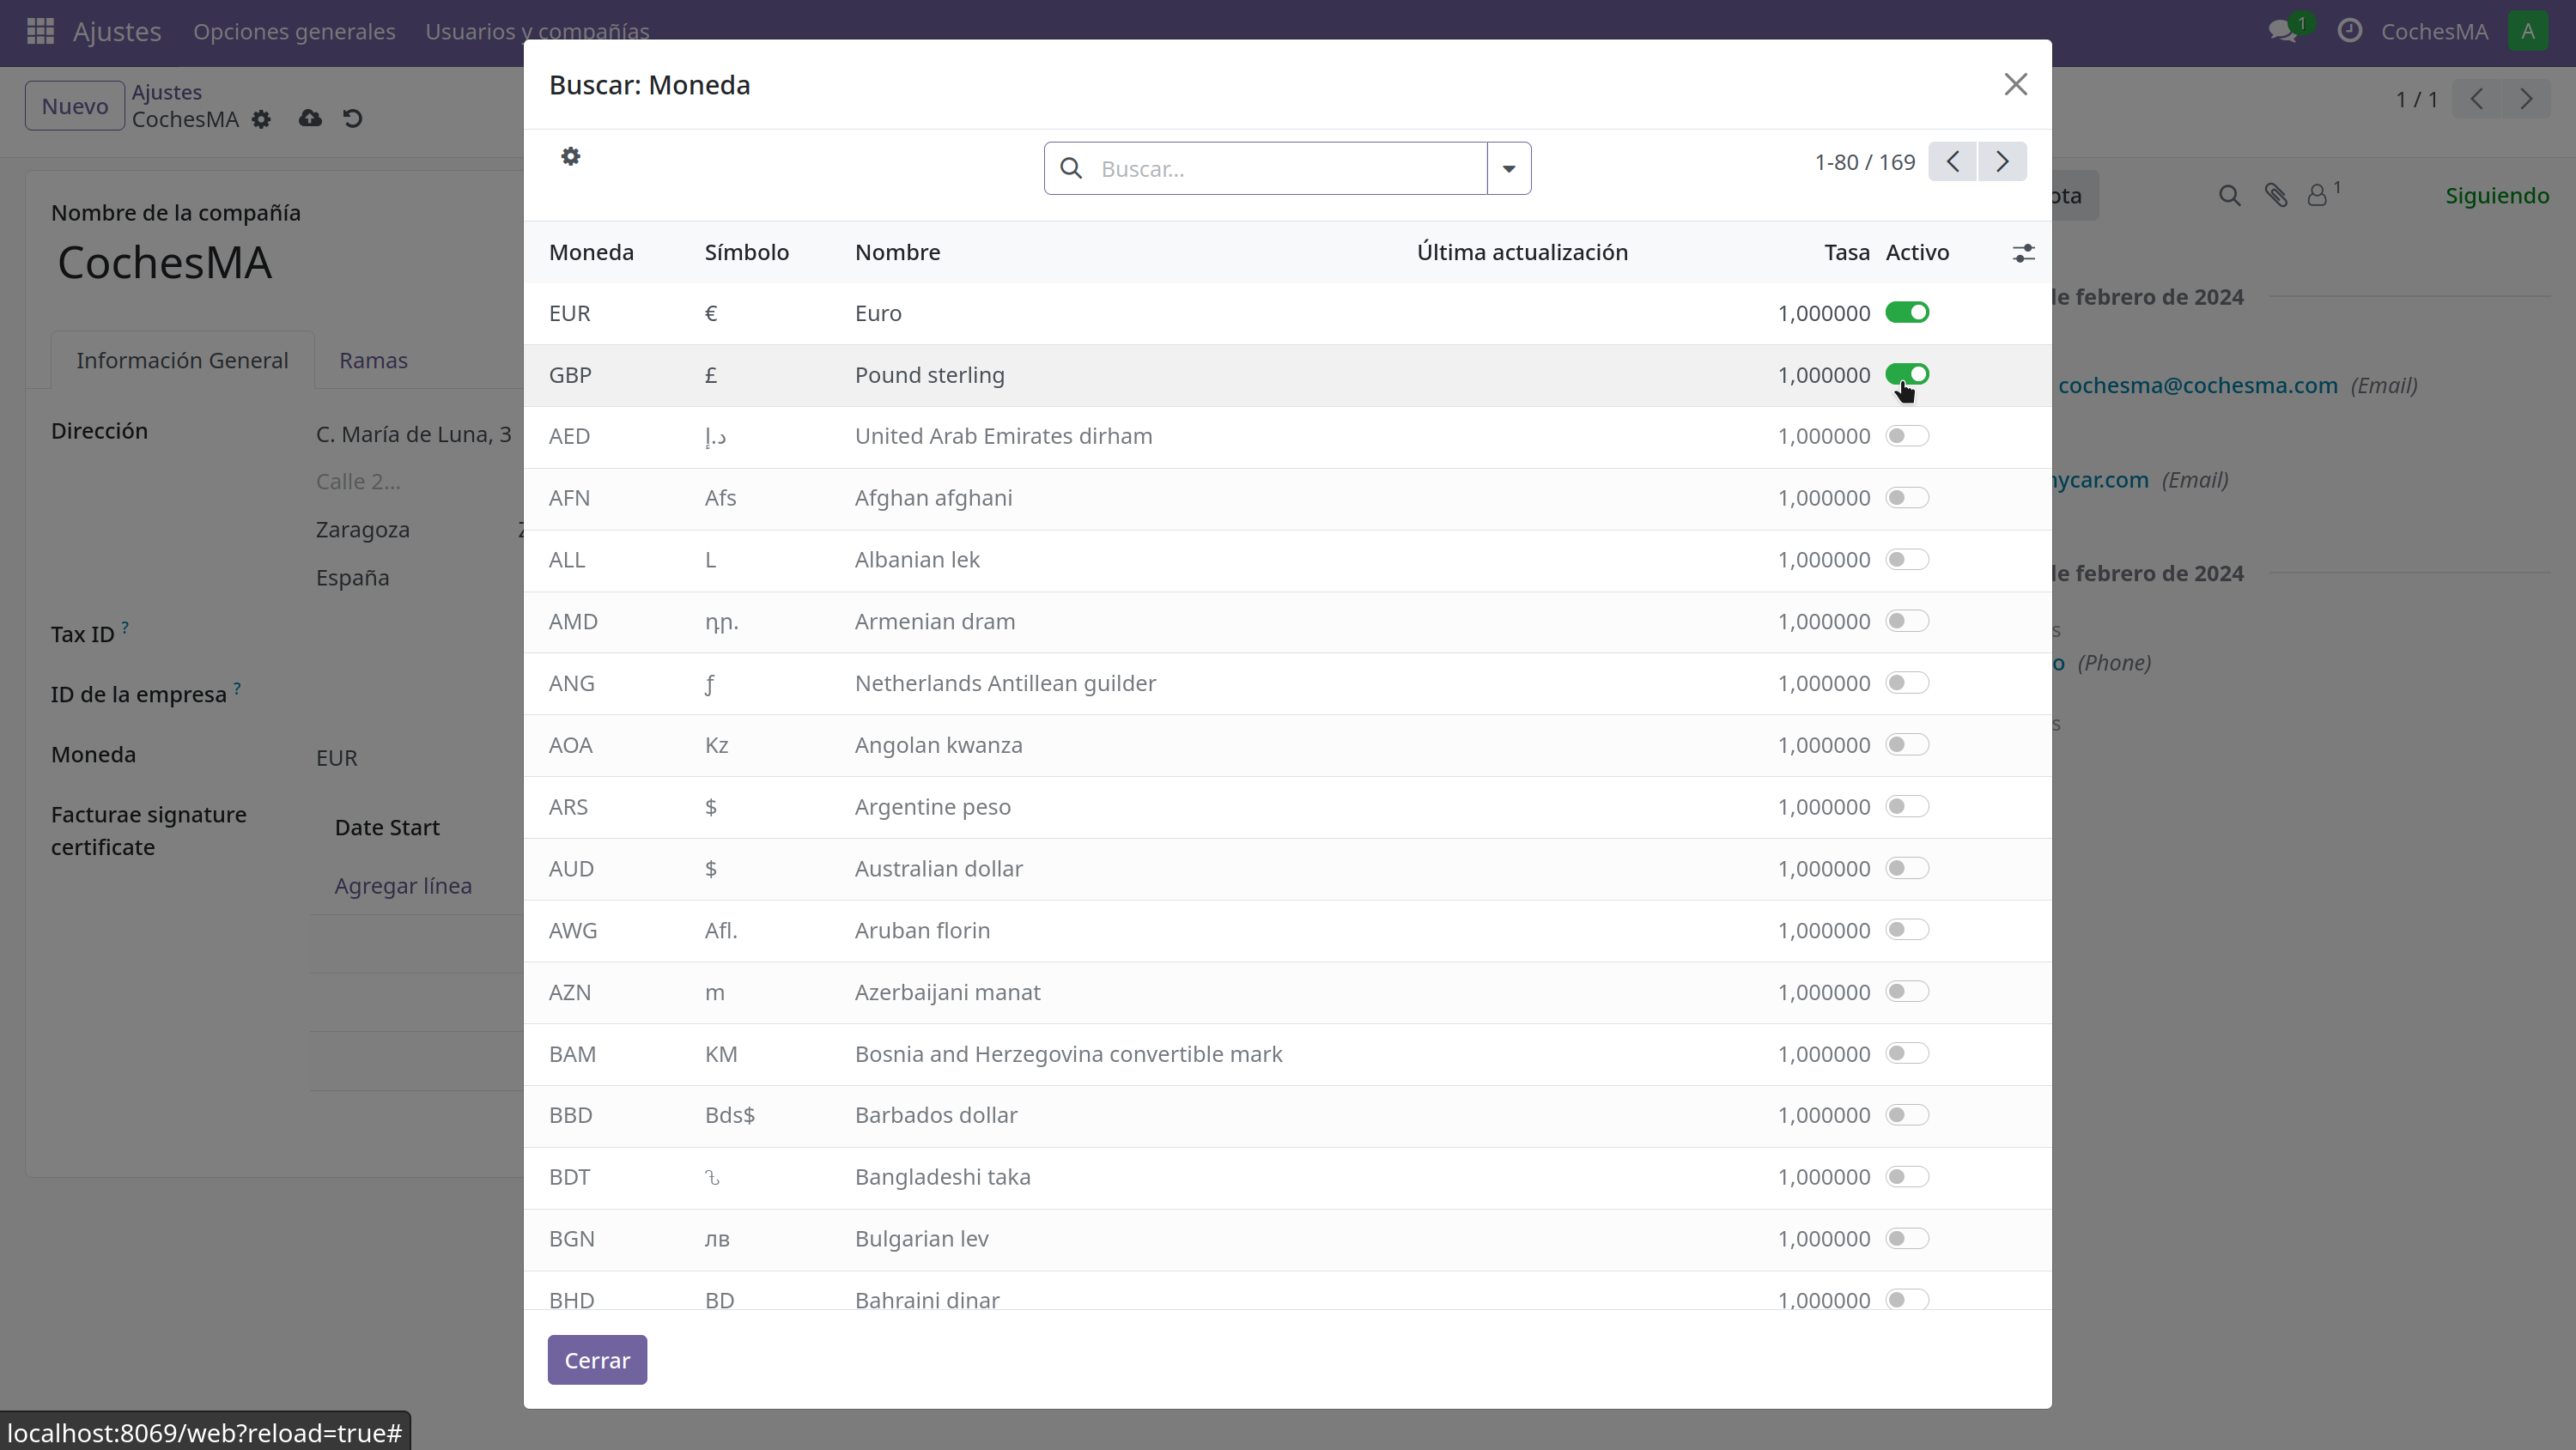
\includegraphics[width=6cm]{currencyMatriz.png}
    \caption{Página para añadir un nuevo tipo de moneda a la compañía matriz.}
    \label{fig:faqs}
\end{figure}
\paragraph{}
Ahora navega a la pestaña de ramas de la compañía matriz y selecciona la compañía rama a la que se quiere añadir la moneda y haz click en el desplegable de la opción Moneda y selecciona Buscar más. Selecciona la moneda que se quiere añadir y pulsa en Guardar.
\begin{figure}[h]
    \centering
    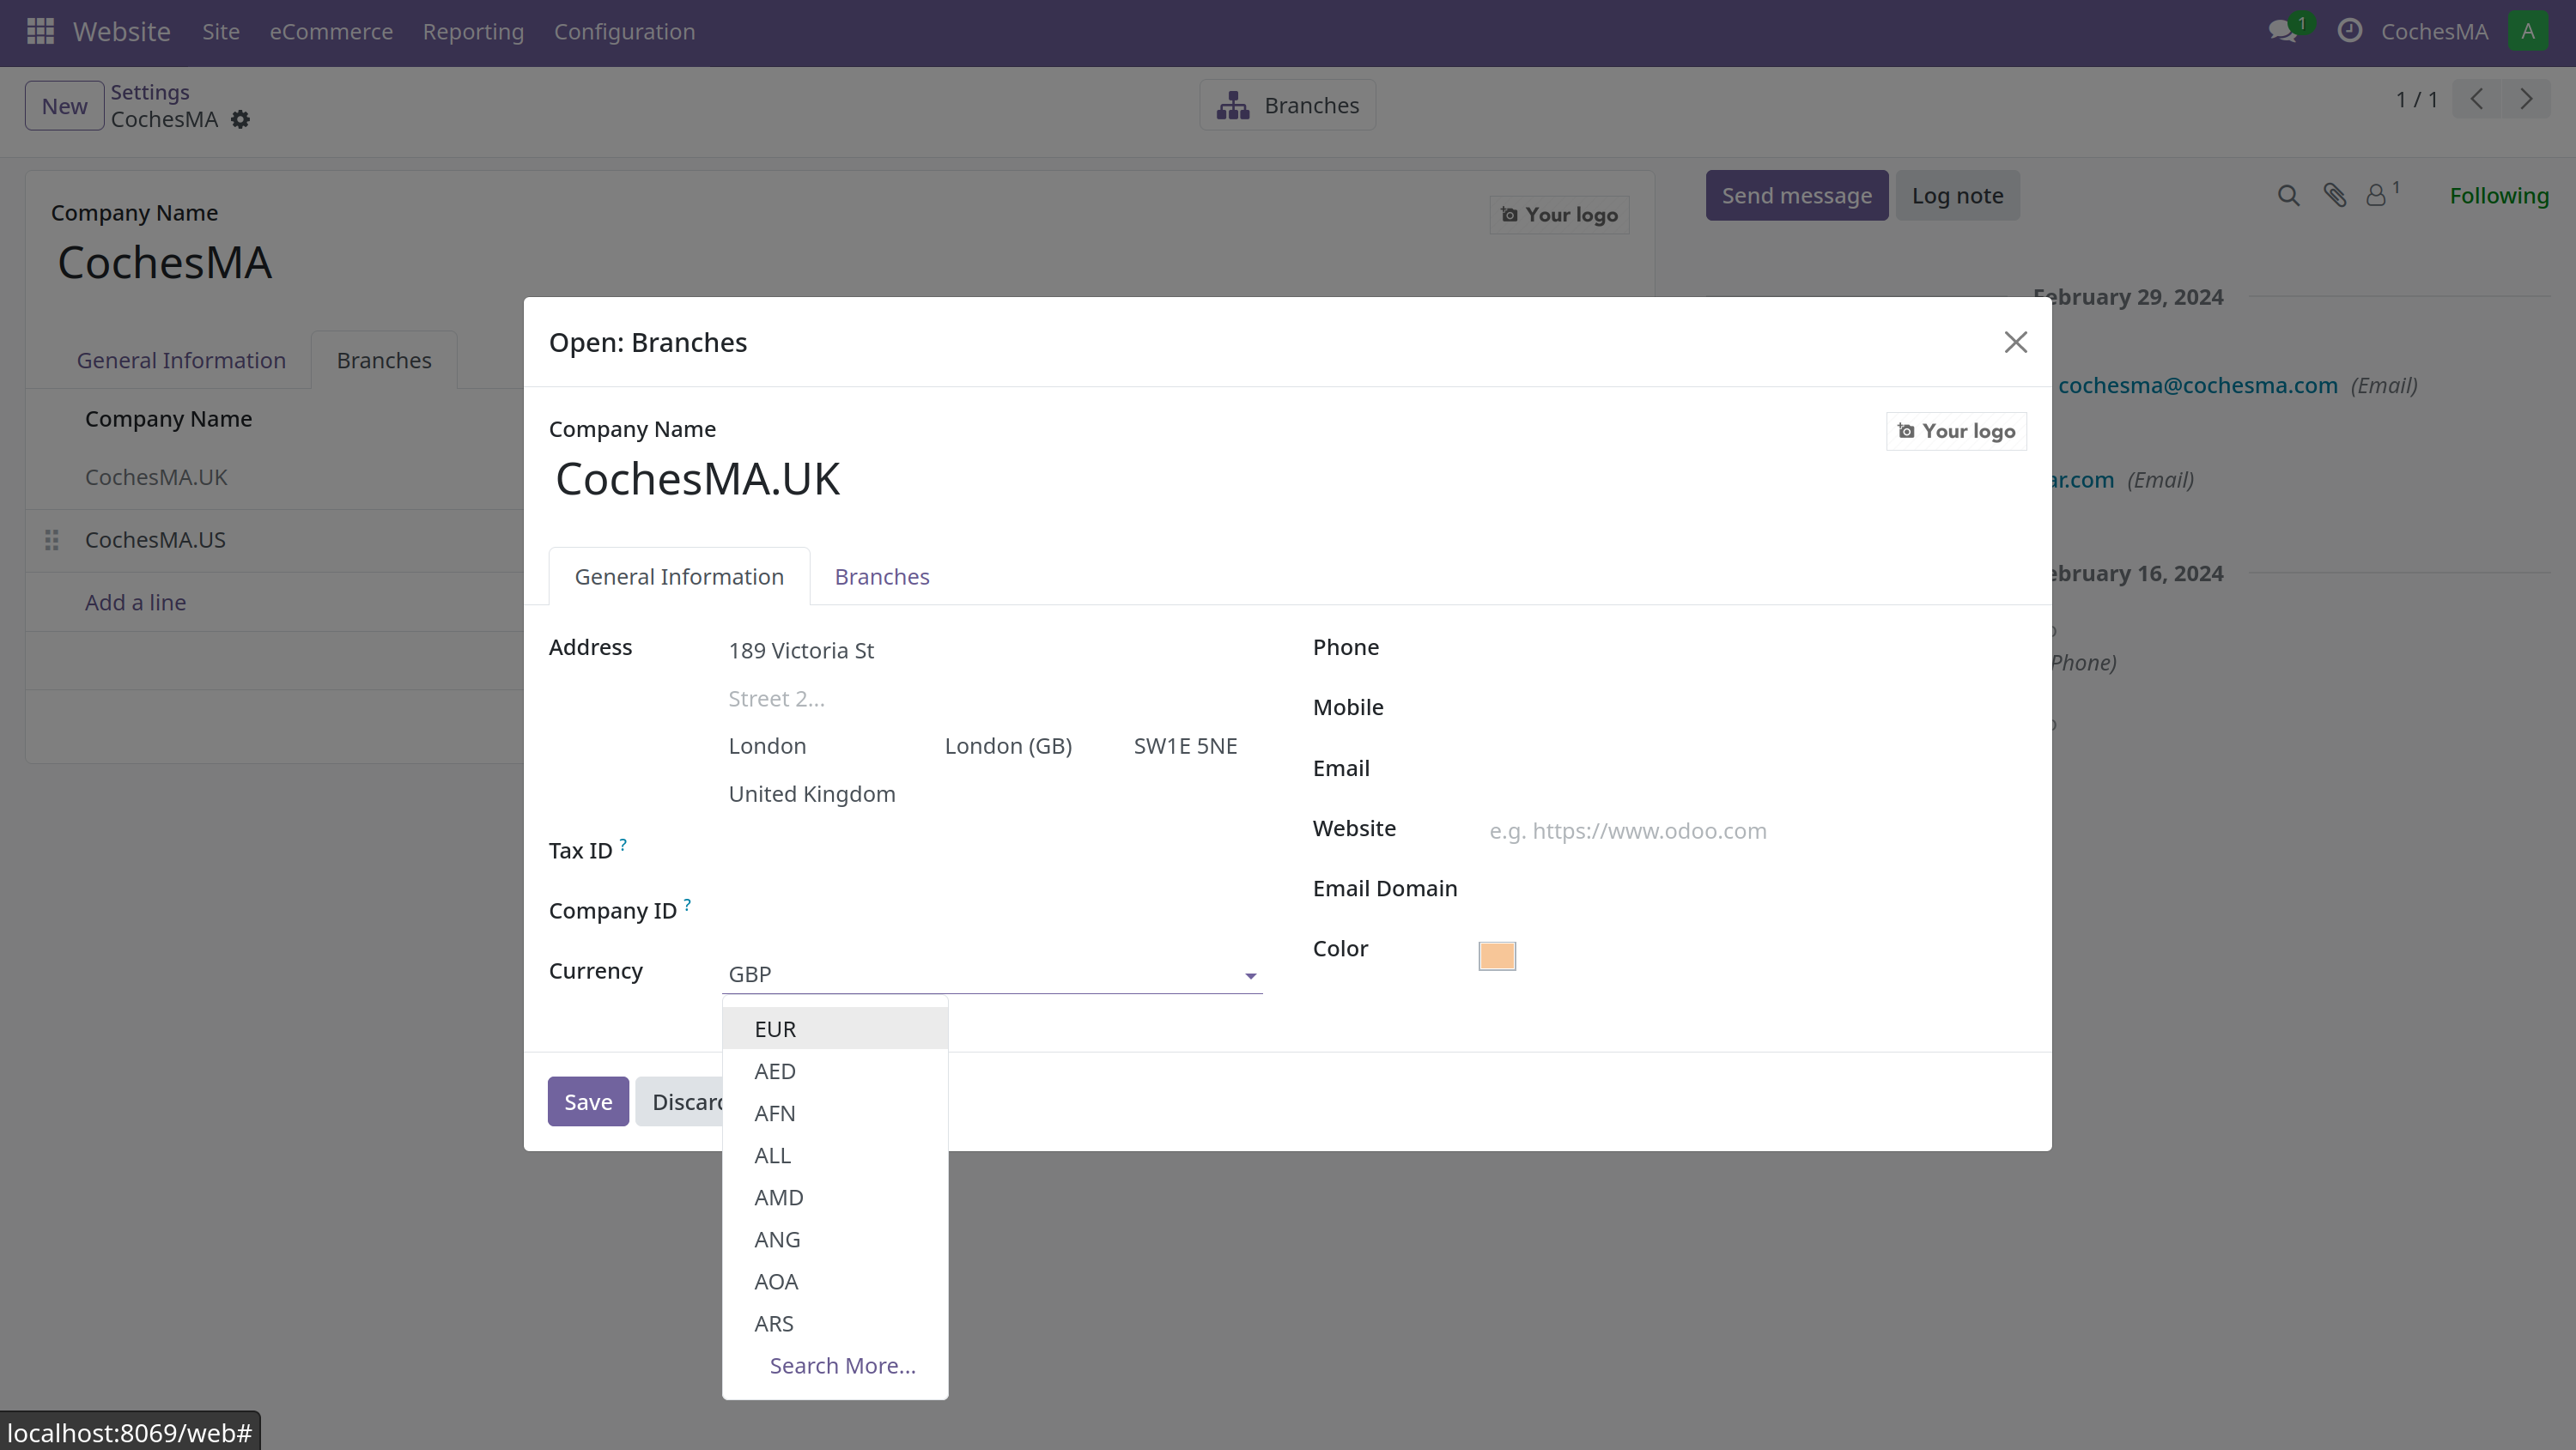
\includegraphics[width=6cm]{currency.png}
    \caption{Página para añadir un nuevo tipo de moneda a las compañías rama.}
    \label{fig:faqs}
\end{figure}
\paragraph{}
Para que cada usuario pueda cambiar el idioma de la pagina web se debe asegurar que los idiomas deseados están en el apartado de sitio web de la configuración y si no añadirlo desde ahi. Solo te dejará añadir idiomas que tengan los usuarios de la compañía.
\newpage
\begin{figure}[h]
    \centering
    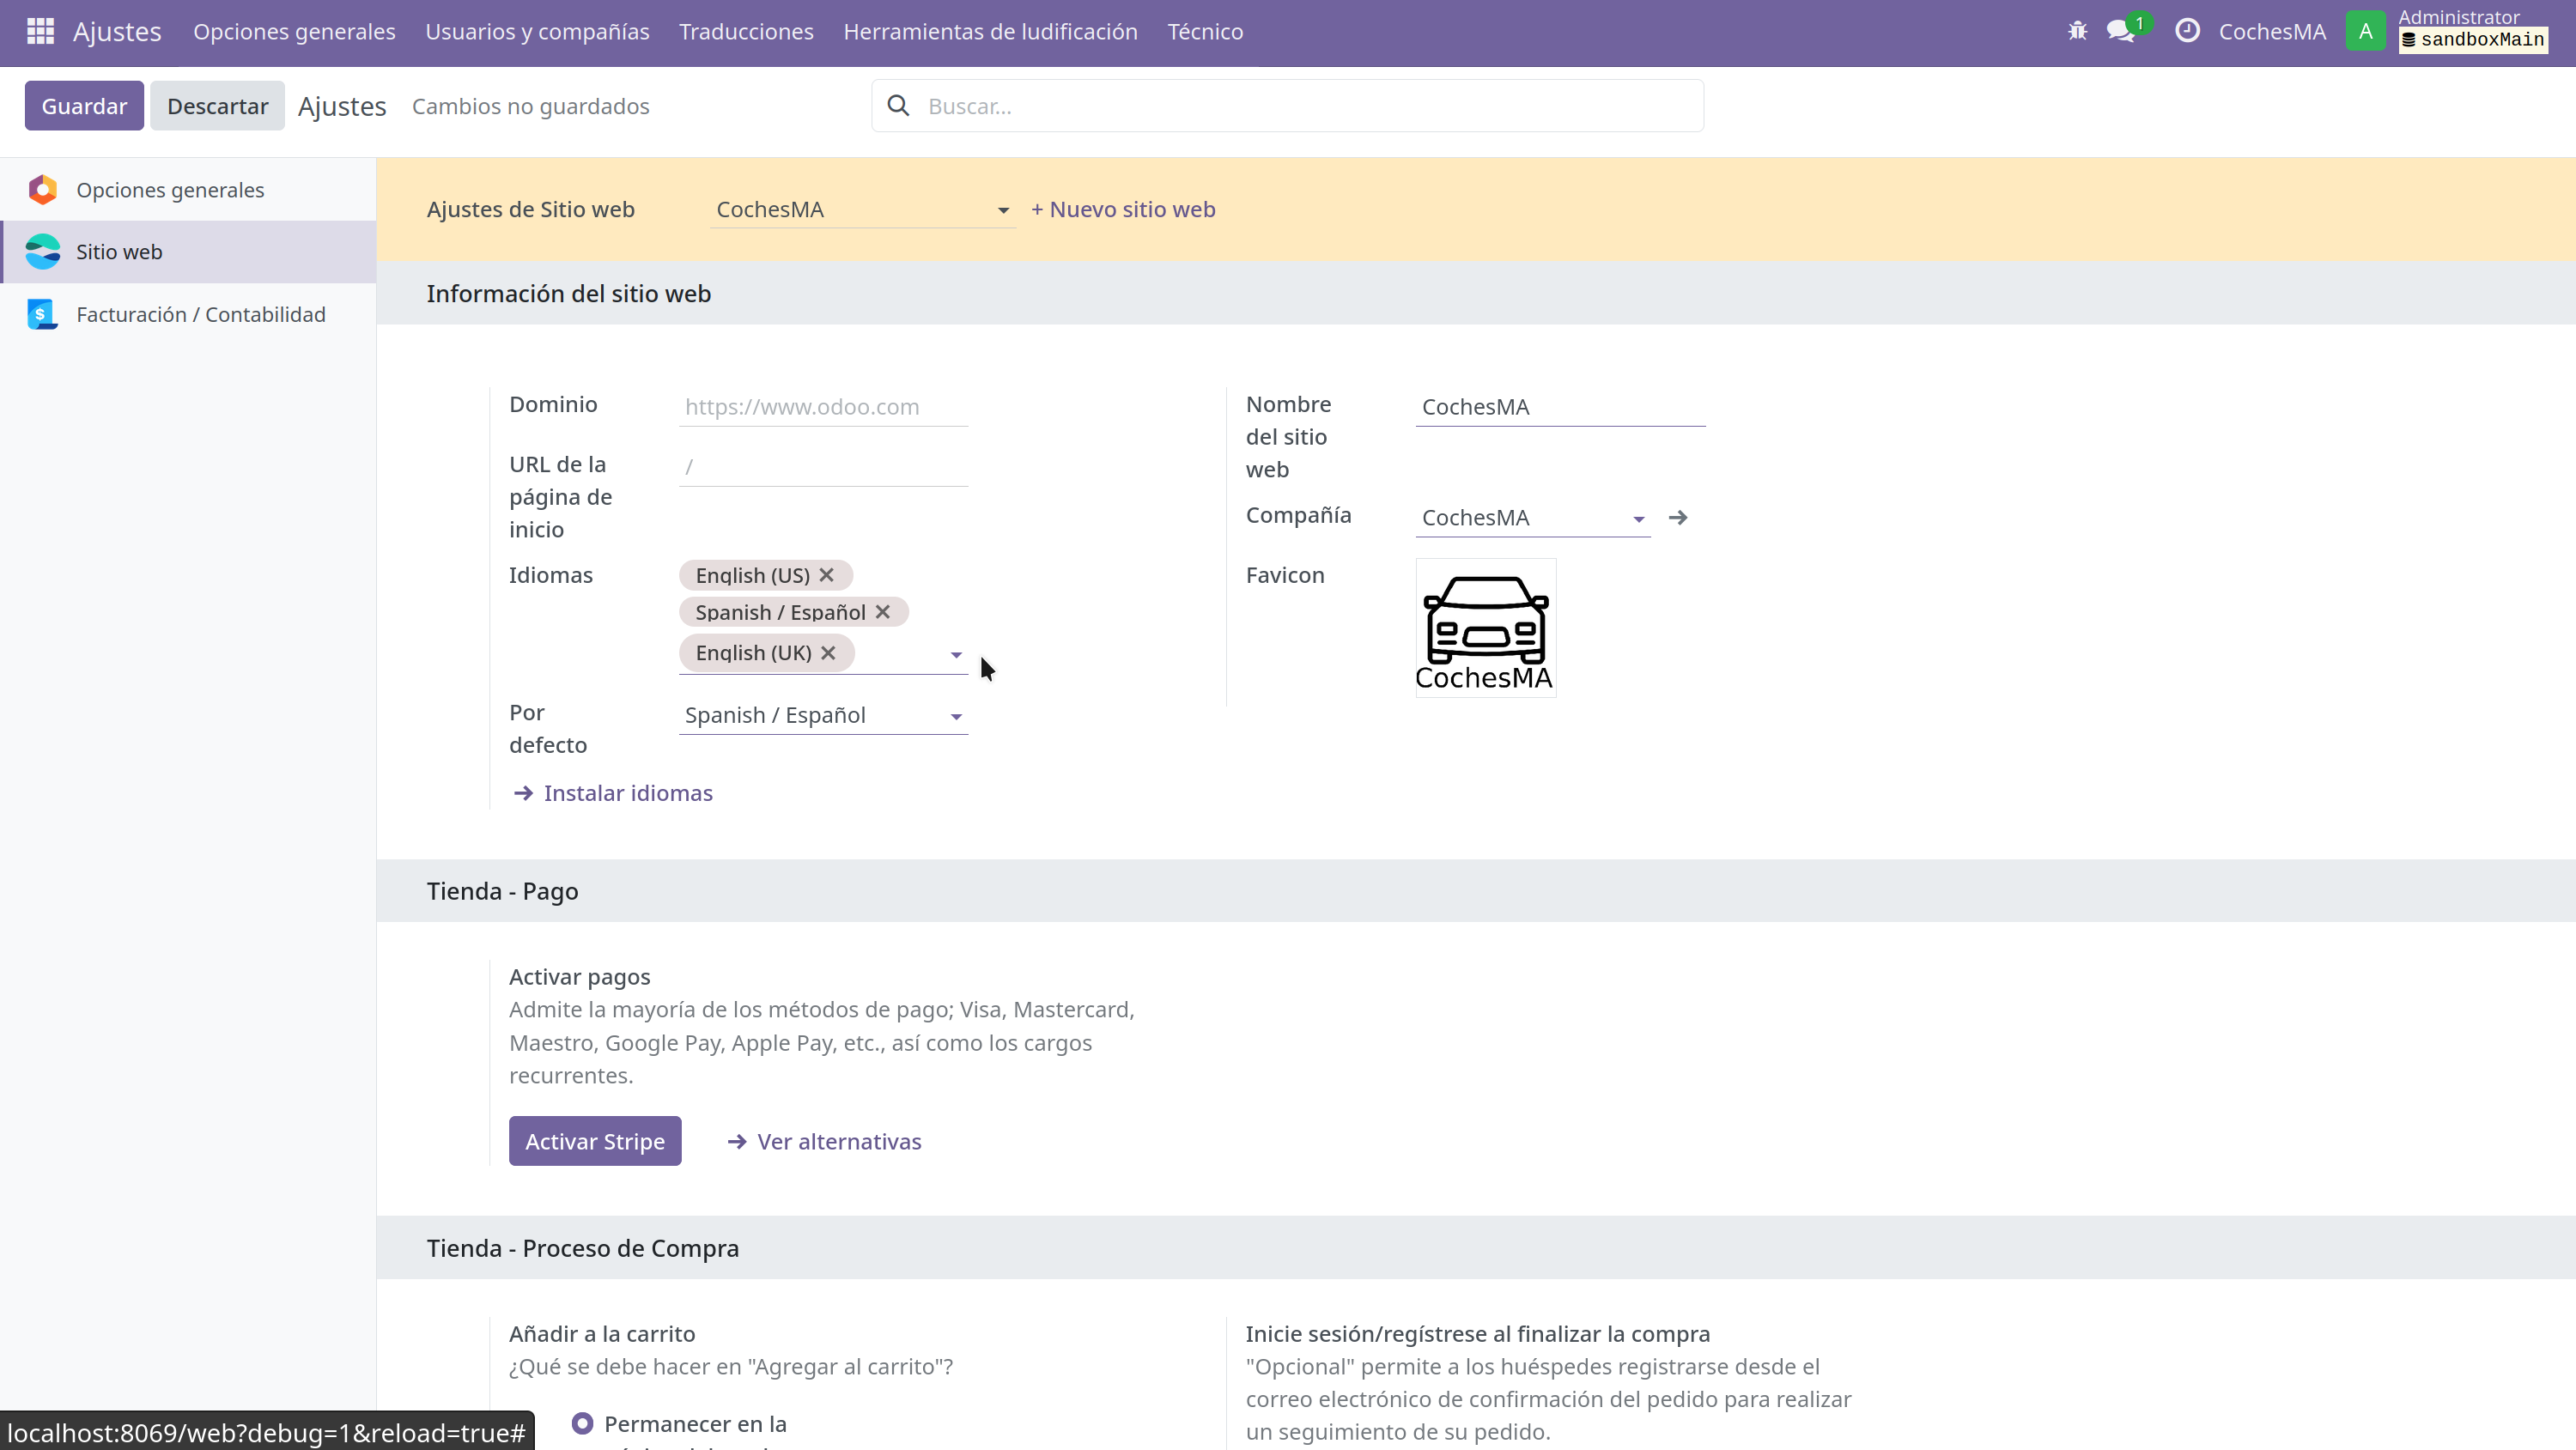
\includegraphics[width=6cm]{idiomasCompañia.png}
    \caption{Página de los idiomas de la web.}
    \label{fig:faqs}
\end{figure}
\paragraph{}
Ahora el usuario podrá cambiar el idioma desde la web en la parte inferior de esta.
\begin{figure}[h]
    \centering
    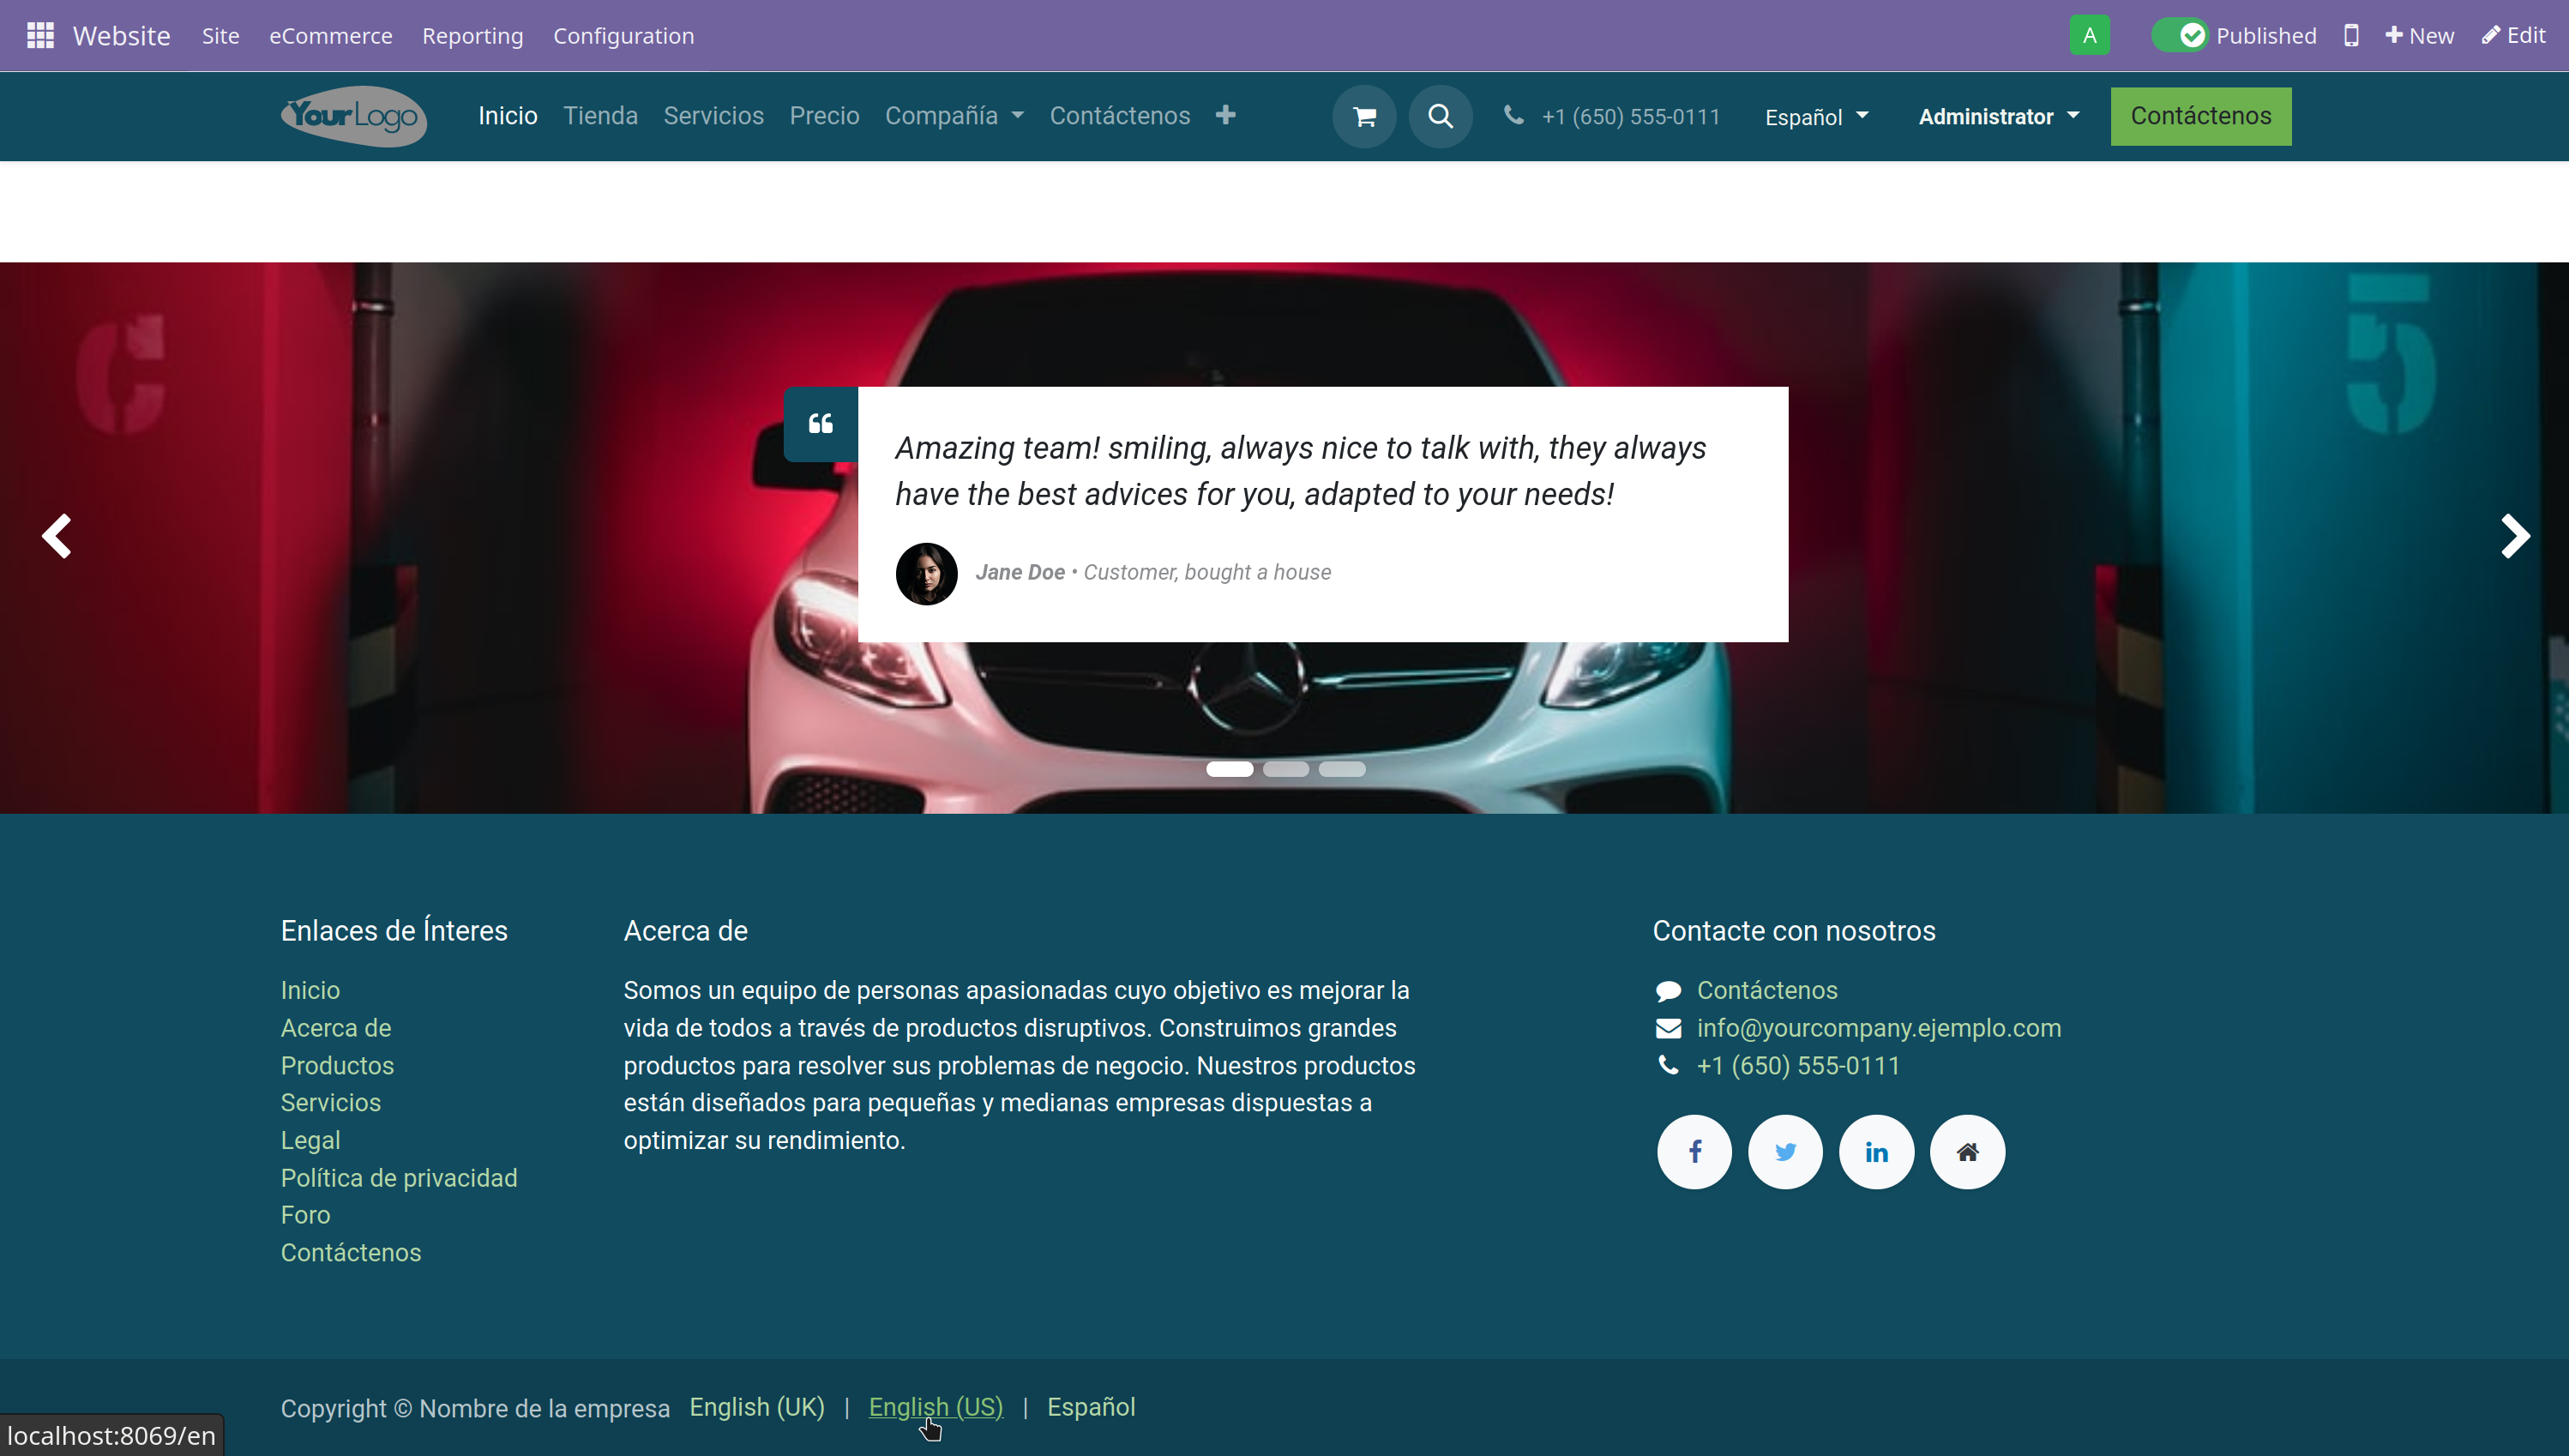
\includegraphics[width=6cm]{idiomasWeb.png}
    \caption{Cambiar idioma en la web.}
    \label{fig:faqs}
\end{figure}
\paragraph{}
Para añadir a la página web el nombre de la empresa, la dirección, los detalles de contacto y la misión se hace editando la web, añadiendo o editando los bloques que la conforman.
Primero, debemos ir a la web de la siguiente manera.
\begin{figure}[h]
    \centering
    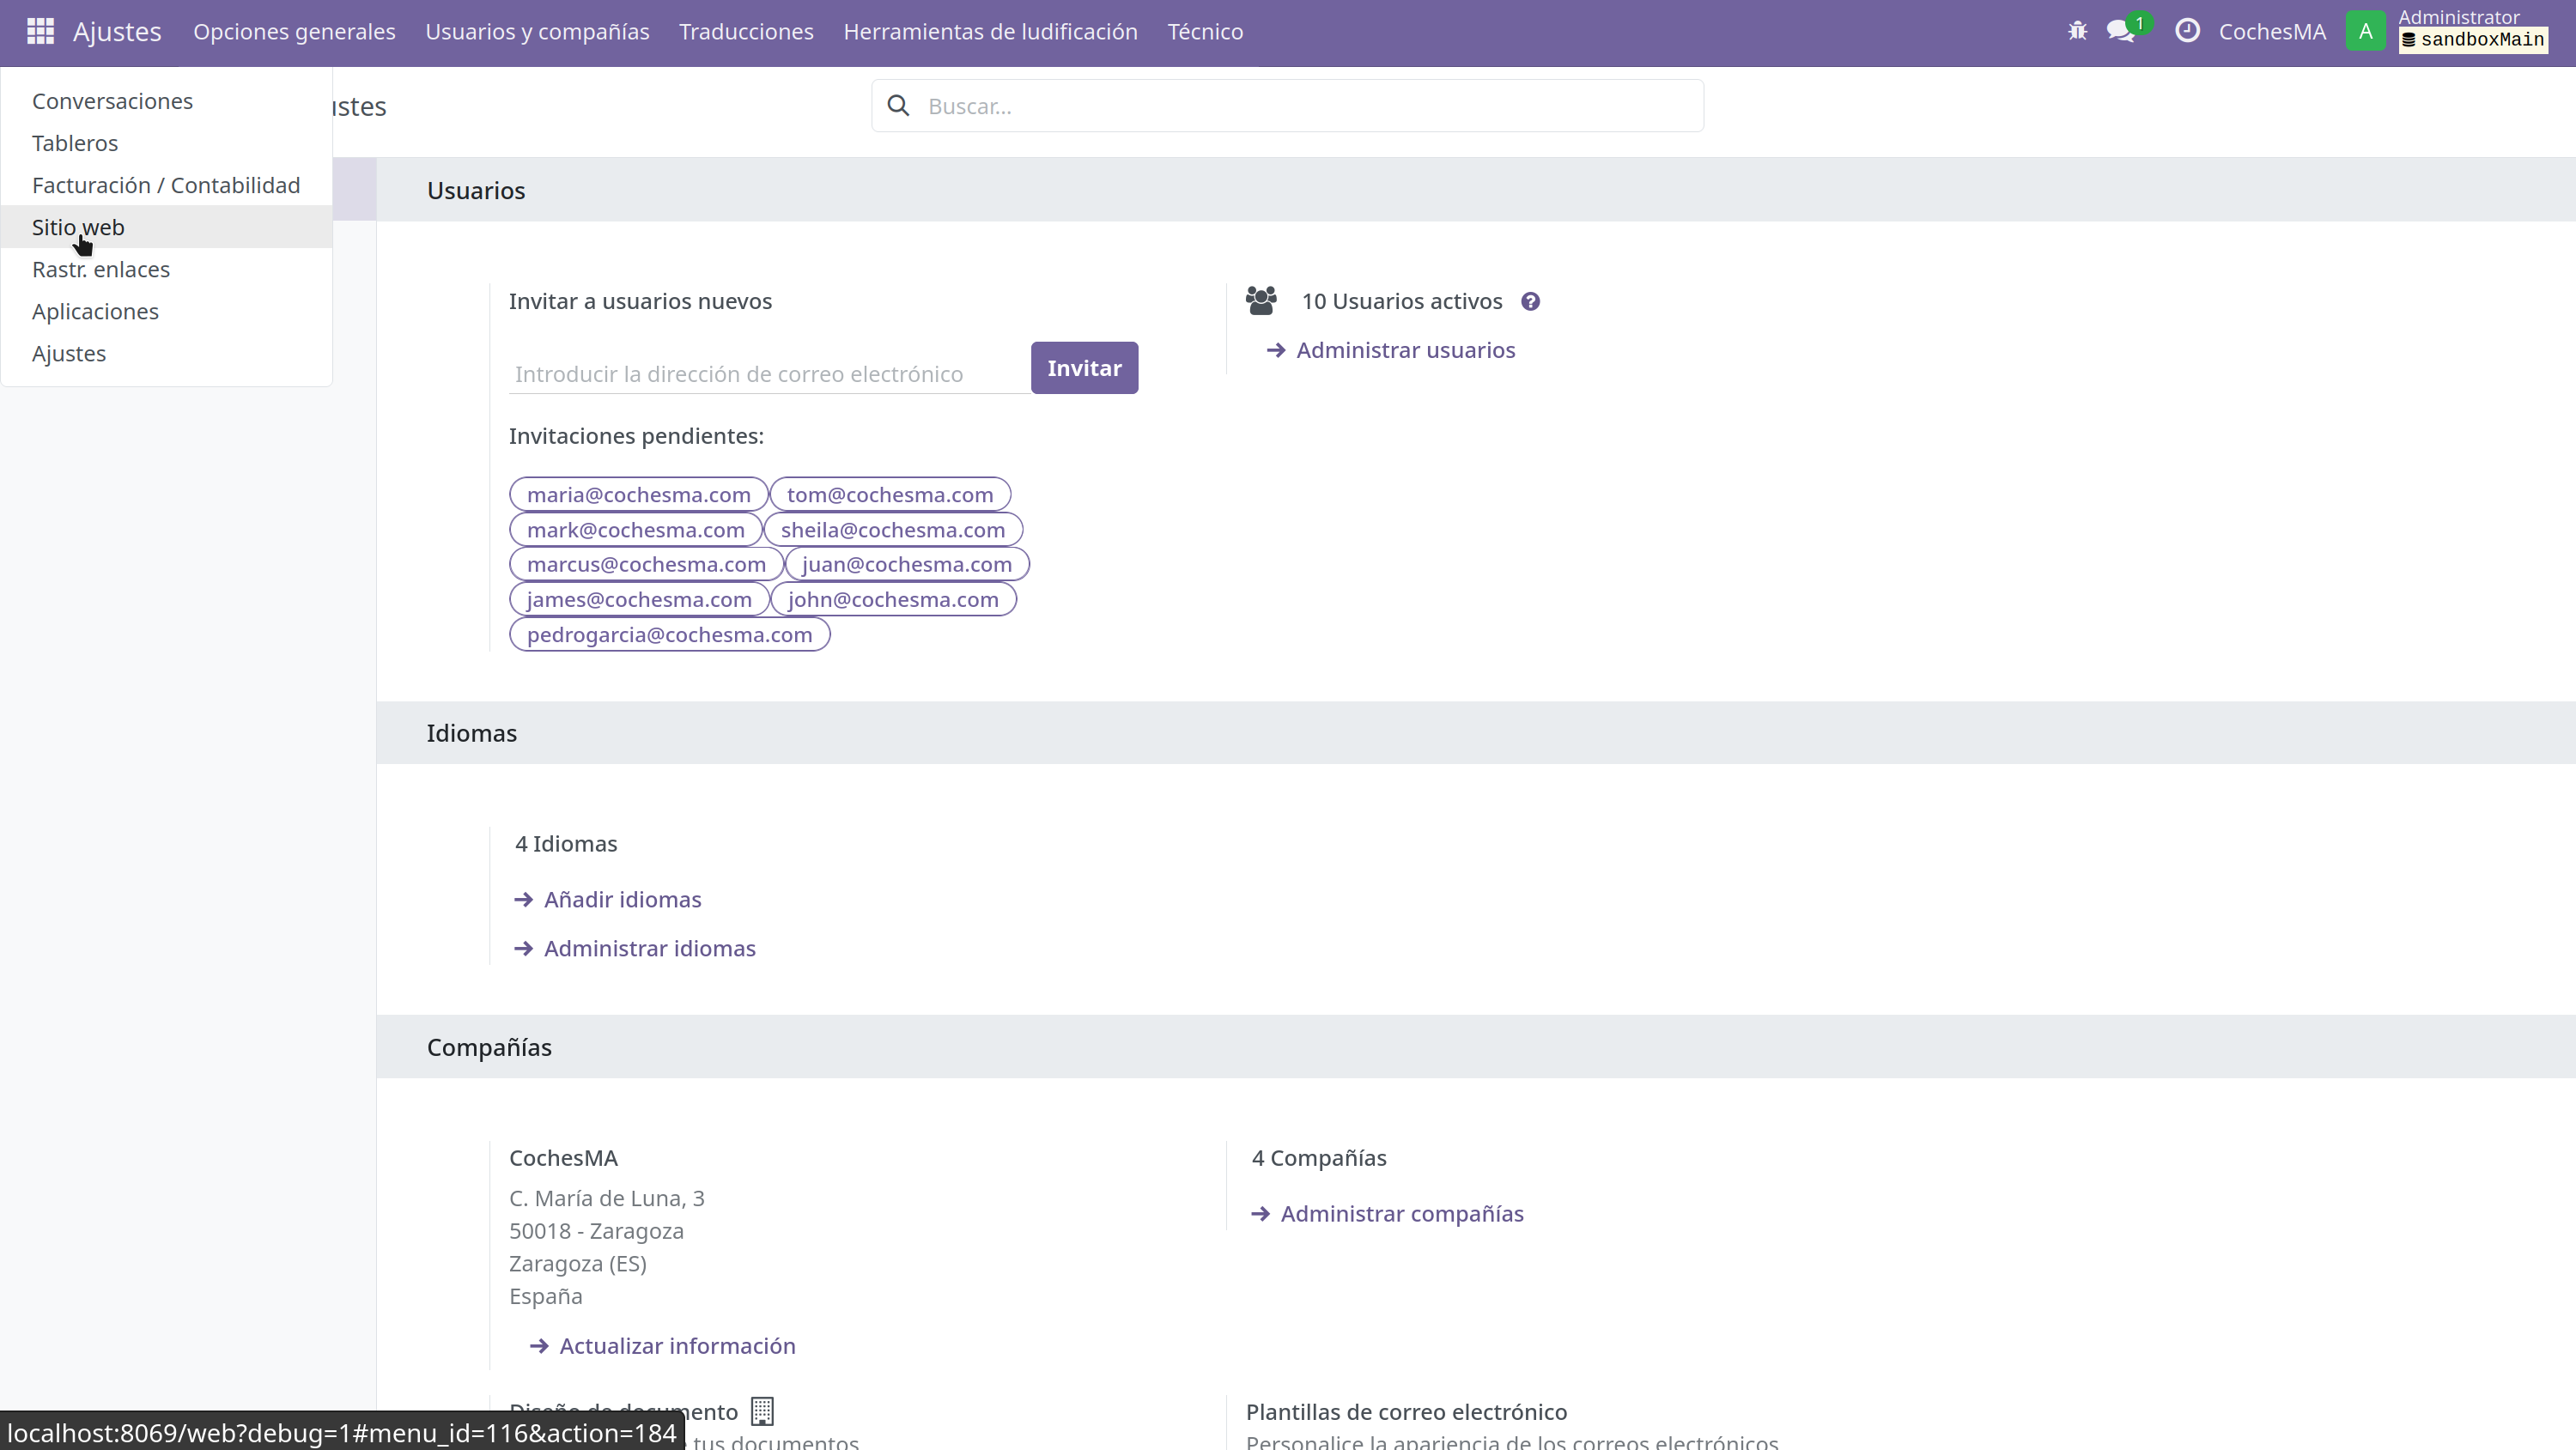
\includegraphics[width=6cm]{sitioWeb.png}
    \caption{Entrar en el sitio web.}
    \label{fig:faqs}
\end{figure}
\paragraph{}
En este caso la información que queremos añadir se va a ubicar en la parte inferior de la página web, por lo que se editará el contenido del bloque correspondiente. Para ello selecciona la opción Editar que hay en la esquina superior derecha para entrar en modo edición. A continuación, haz doble click encima del bloque e introduce la información correspondiente.
\newpage
\begin{figure}[h]
    \centering
    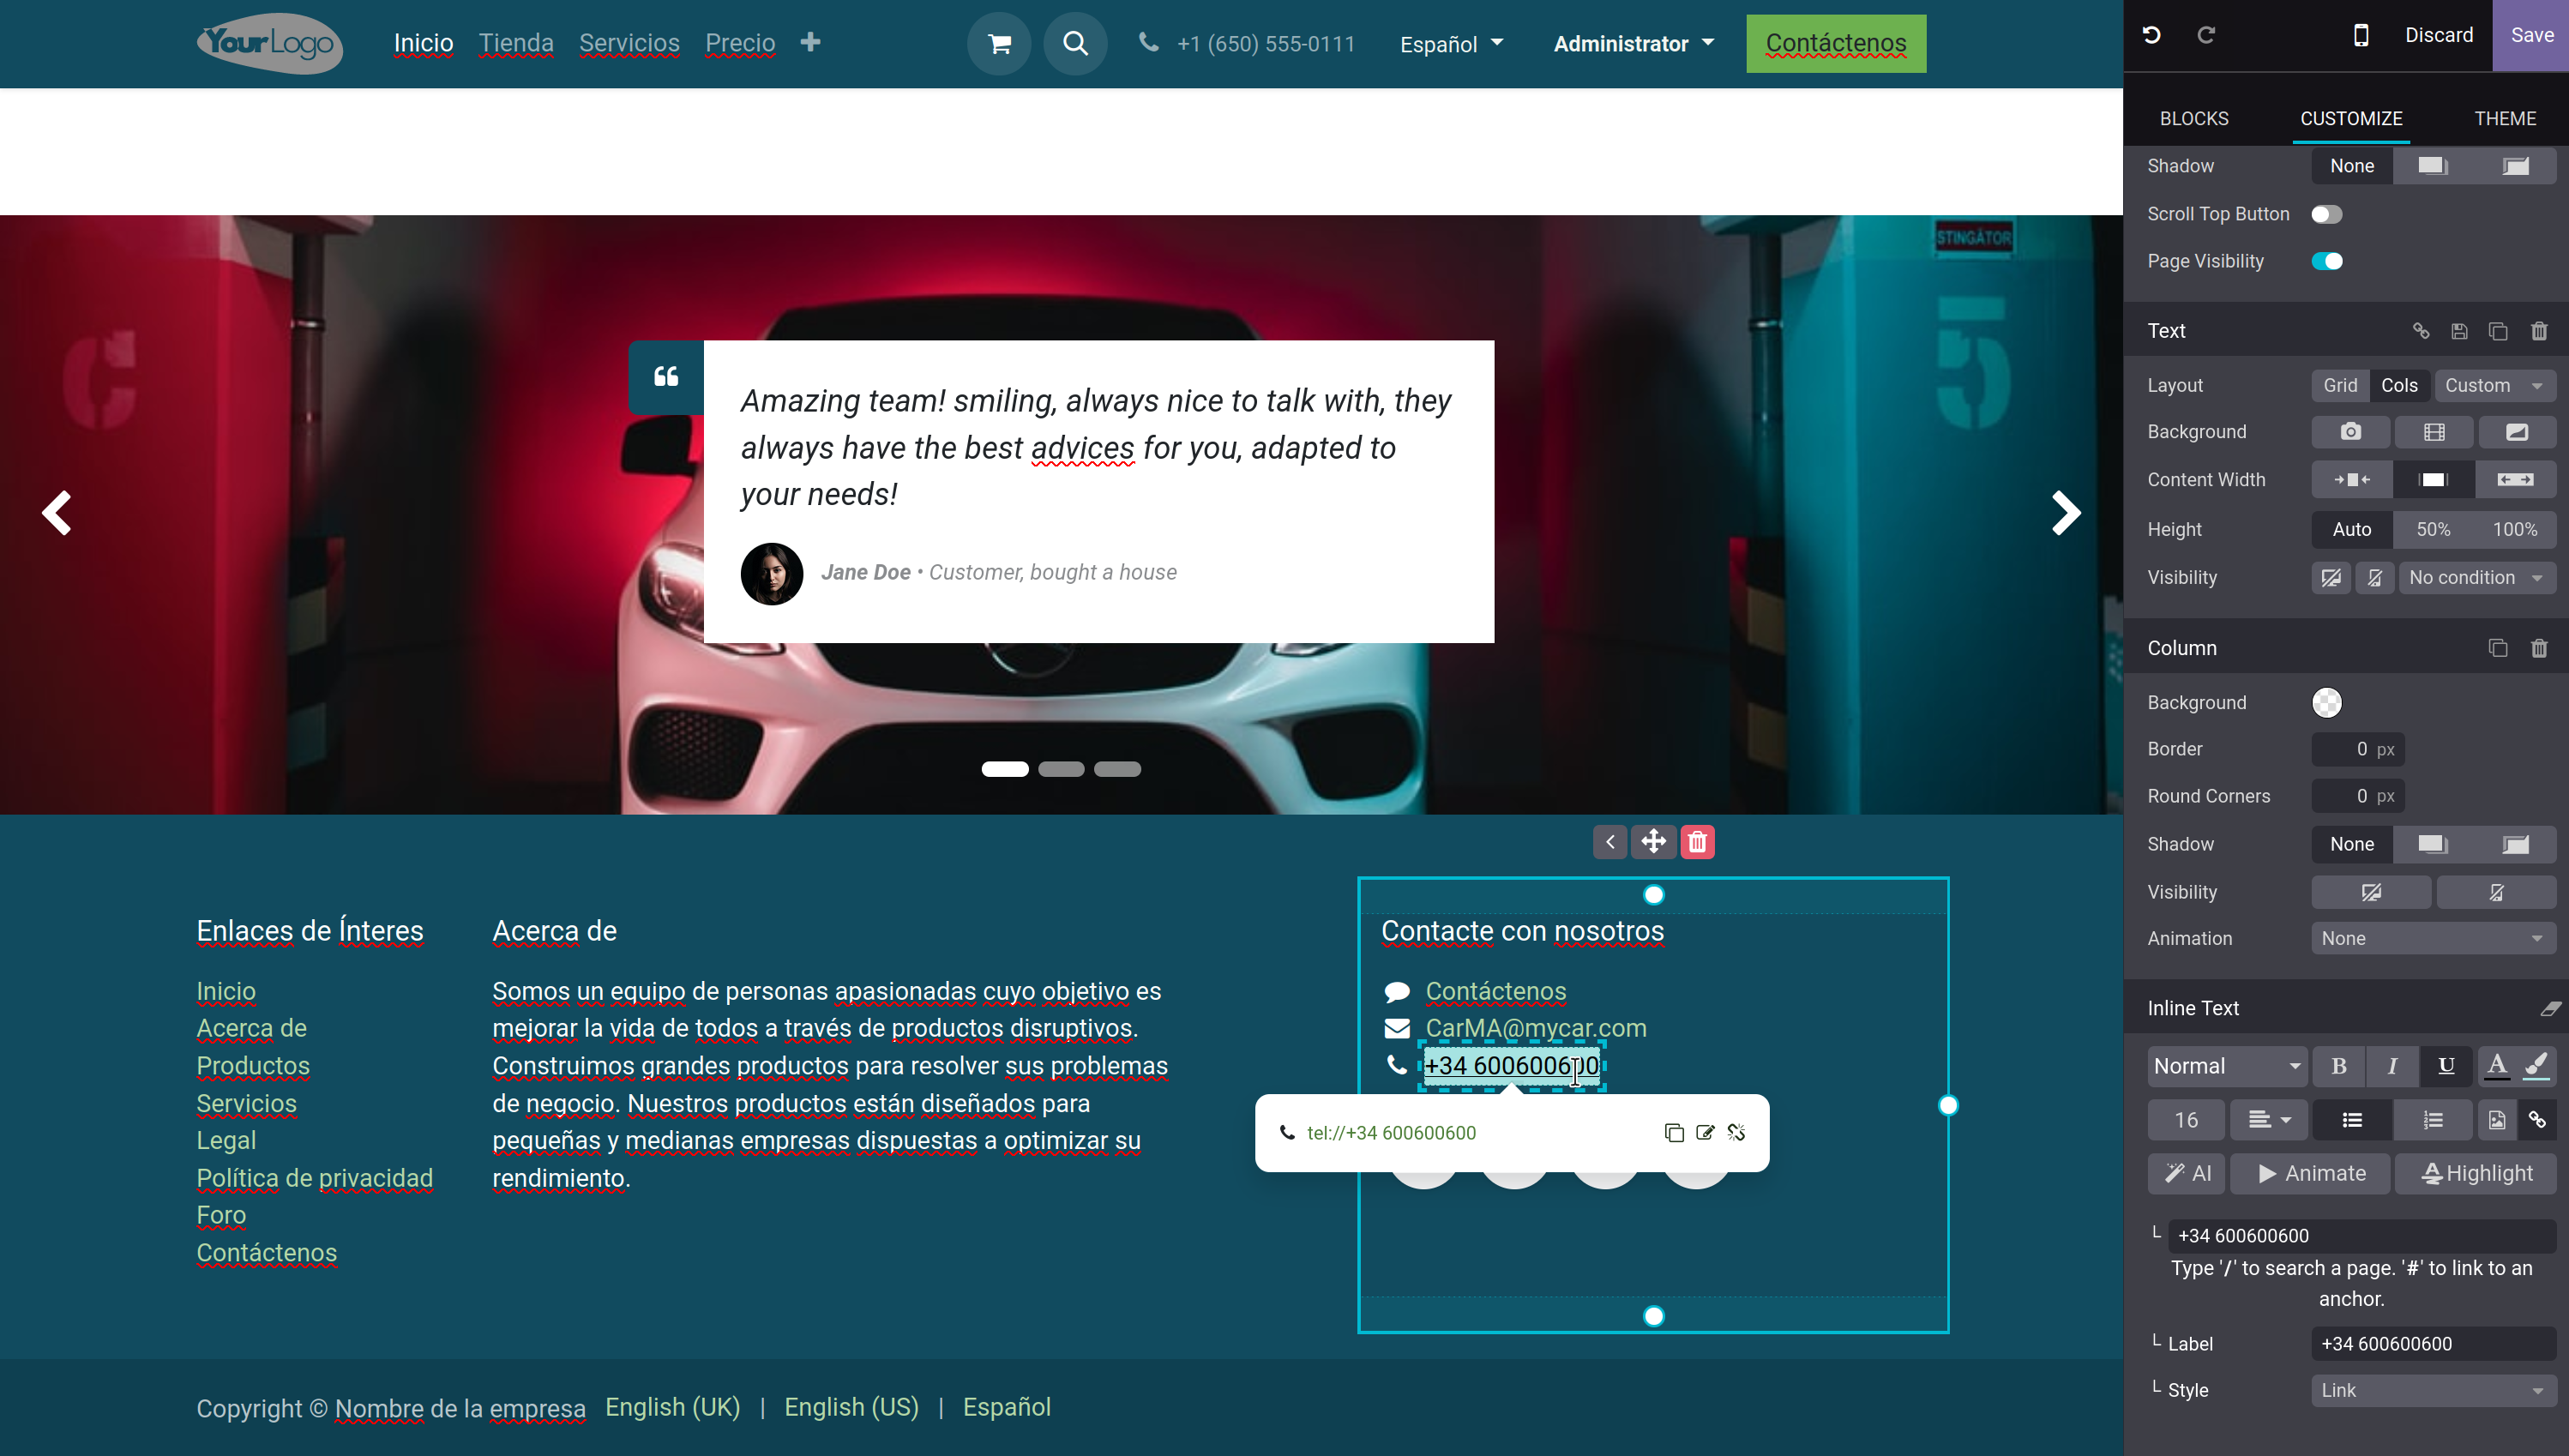
\includegraphics[width=6cm]{añadirInfoCompañia.png}
    \caption{Edición de la información de la compañía en la web.}
    \label{fig:faqs}
\end{figure}
\paragraph{}
Edita todos los bloques deseados en las demás páginas de la web de la misma manera
\begin{figure}[h]
    \centering
    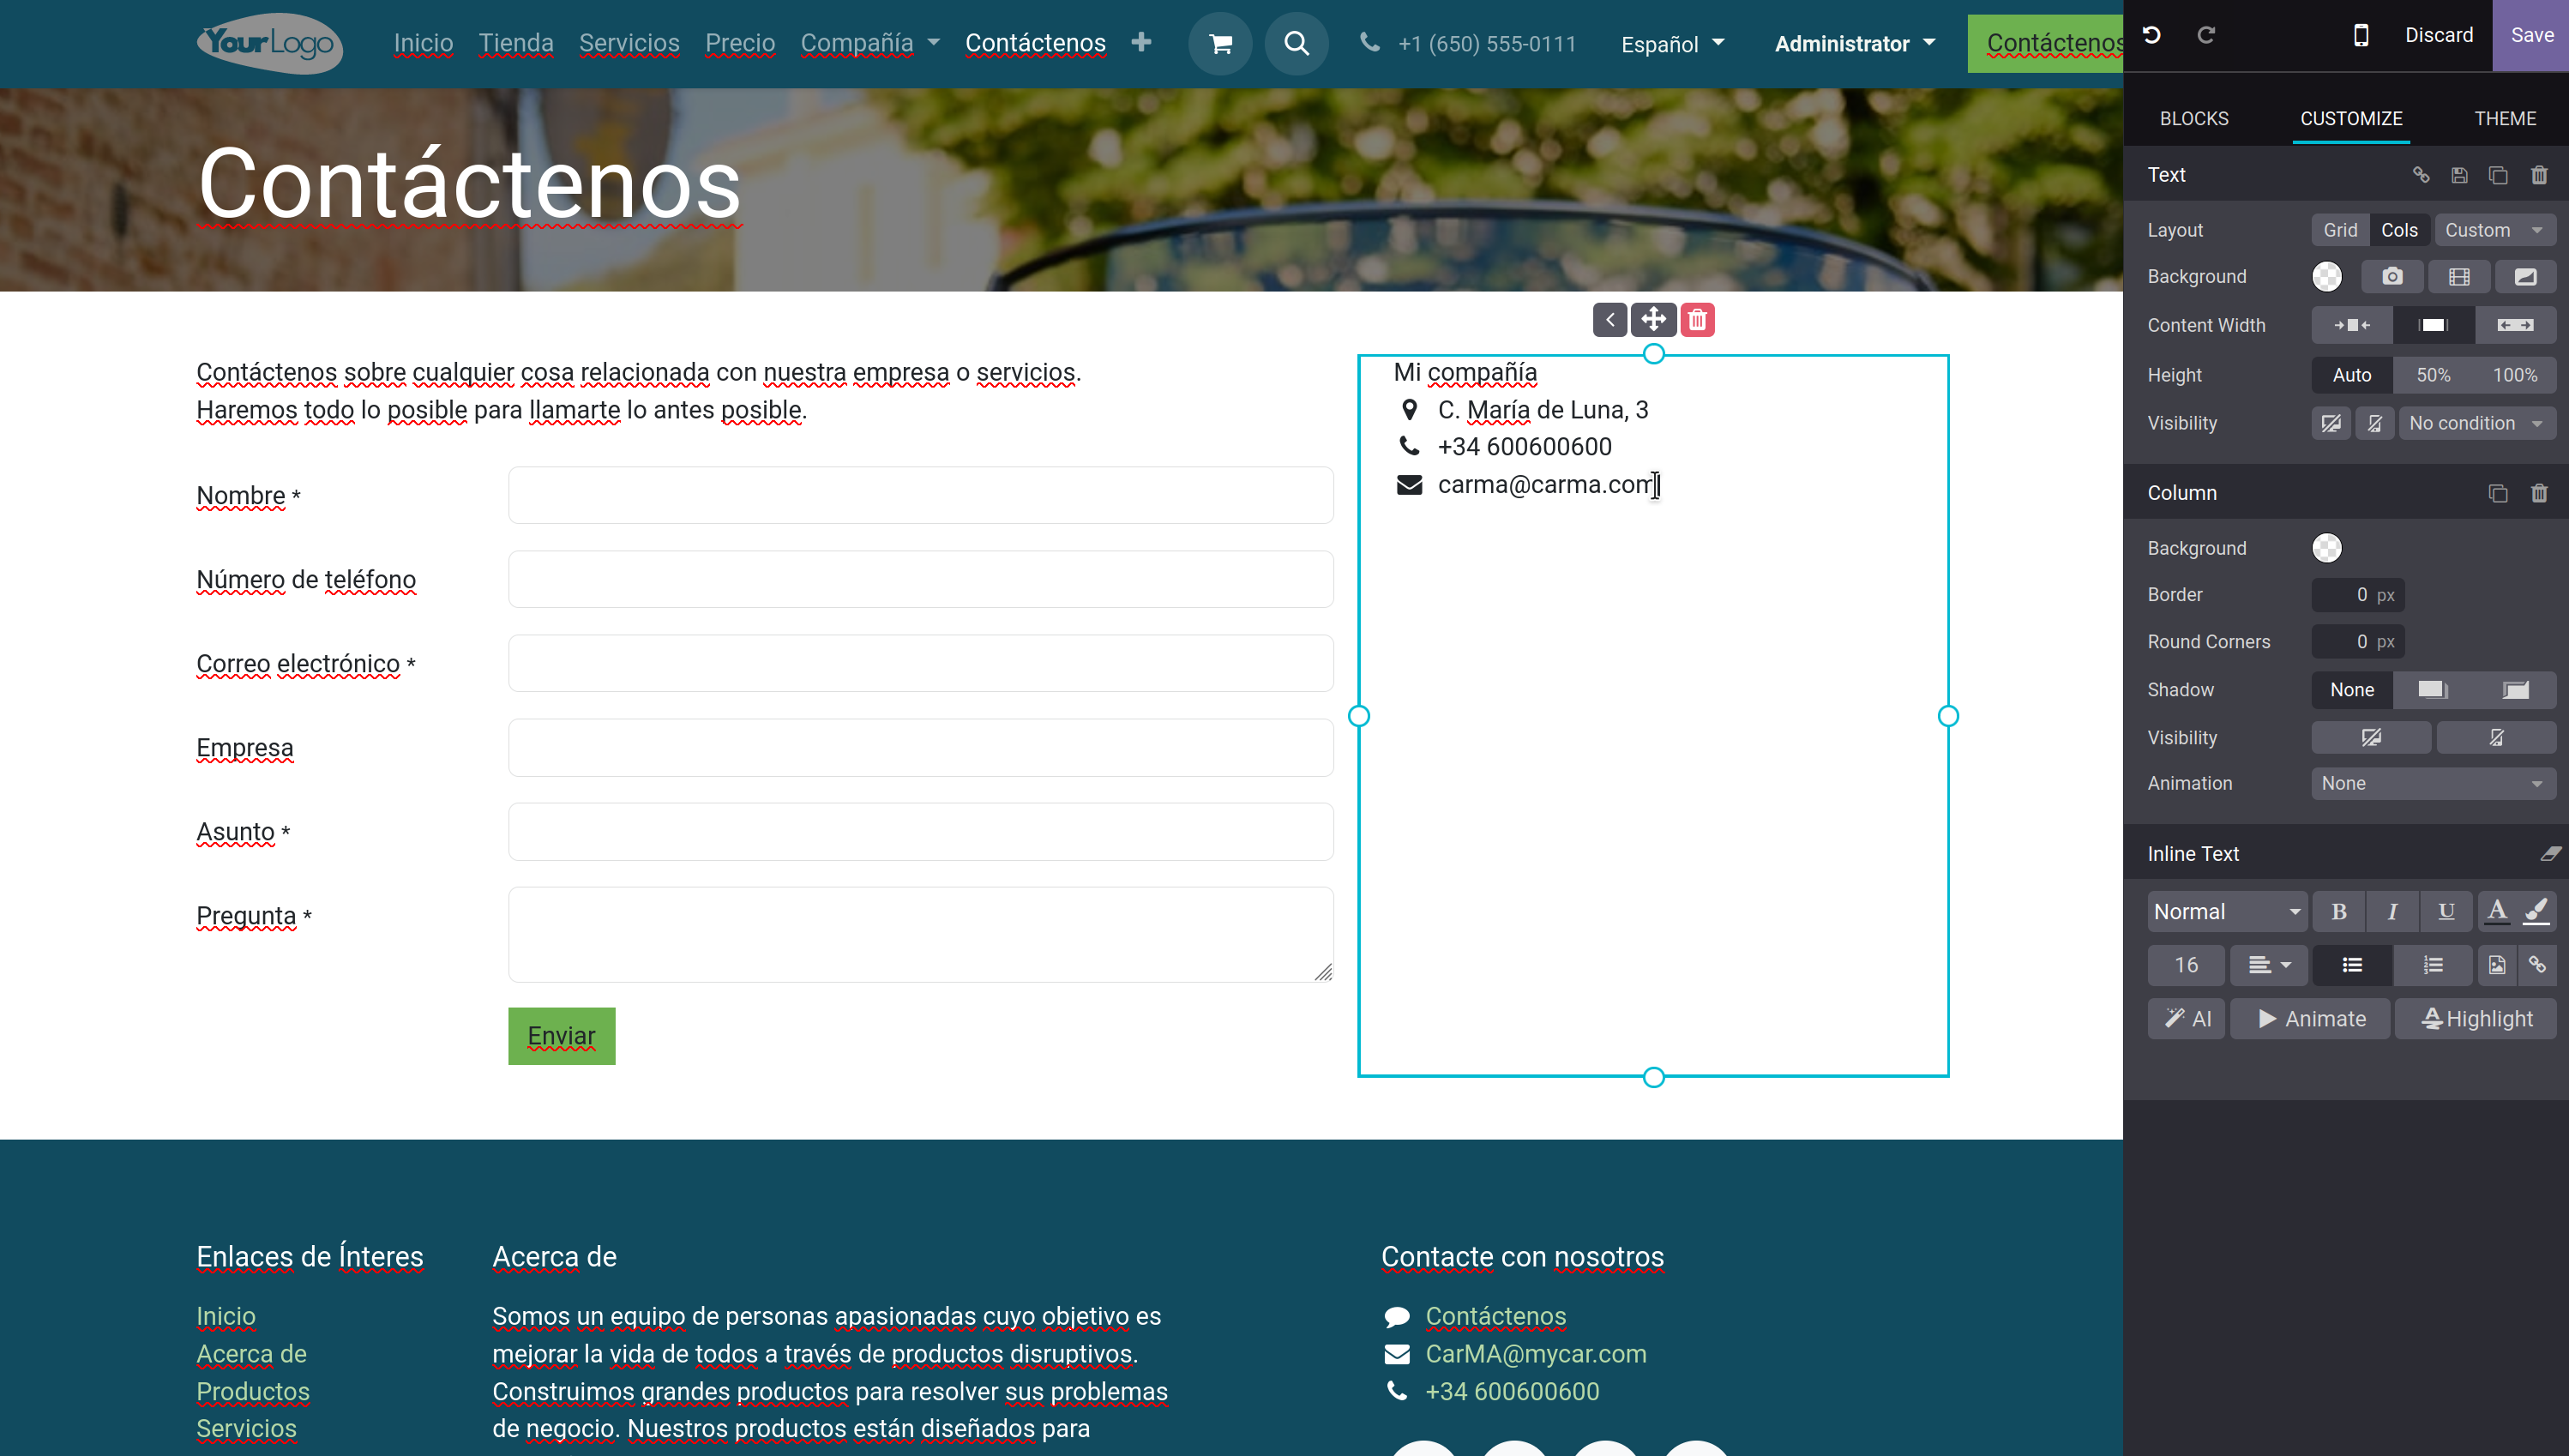
\includegraphics[width=6cm]{añadirInfoCompañia2.png}
    \caption{Edición de la información de la compañía en la web.}
    \label{fig:faqs}
\end{figure}
\begin{figure}[h]
    \centering
    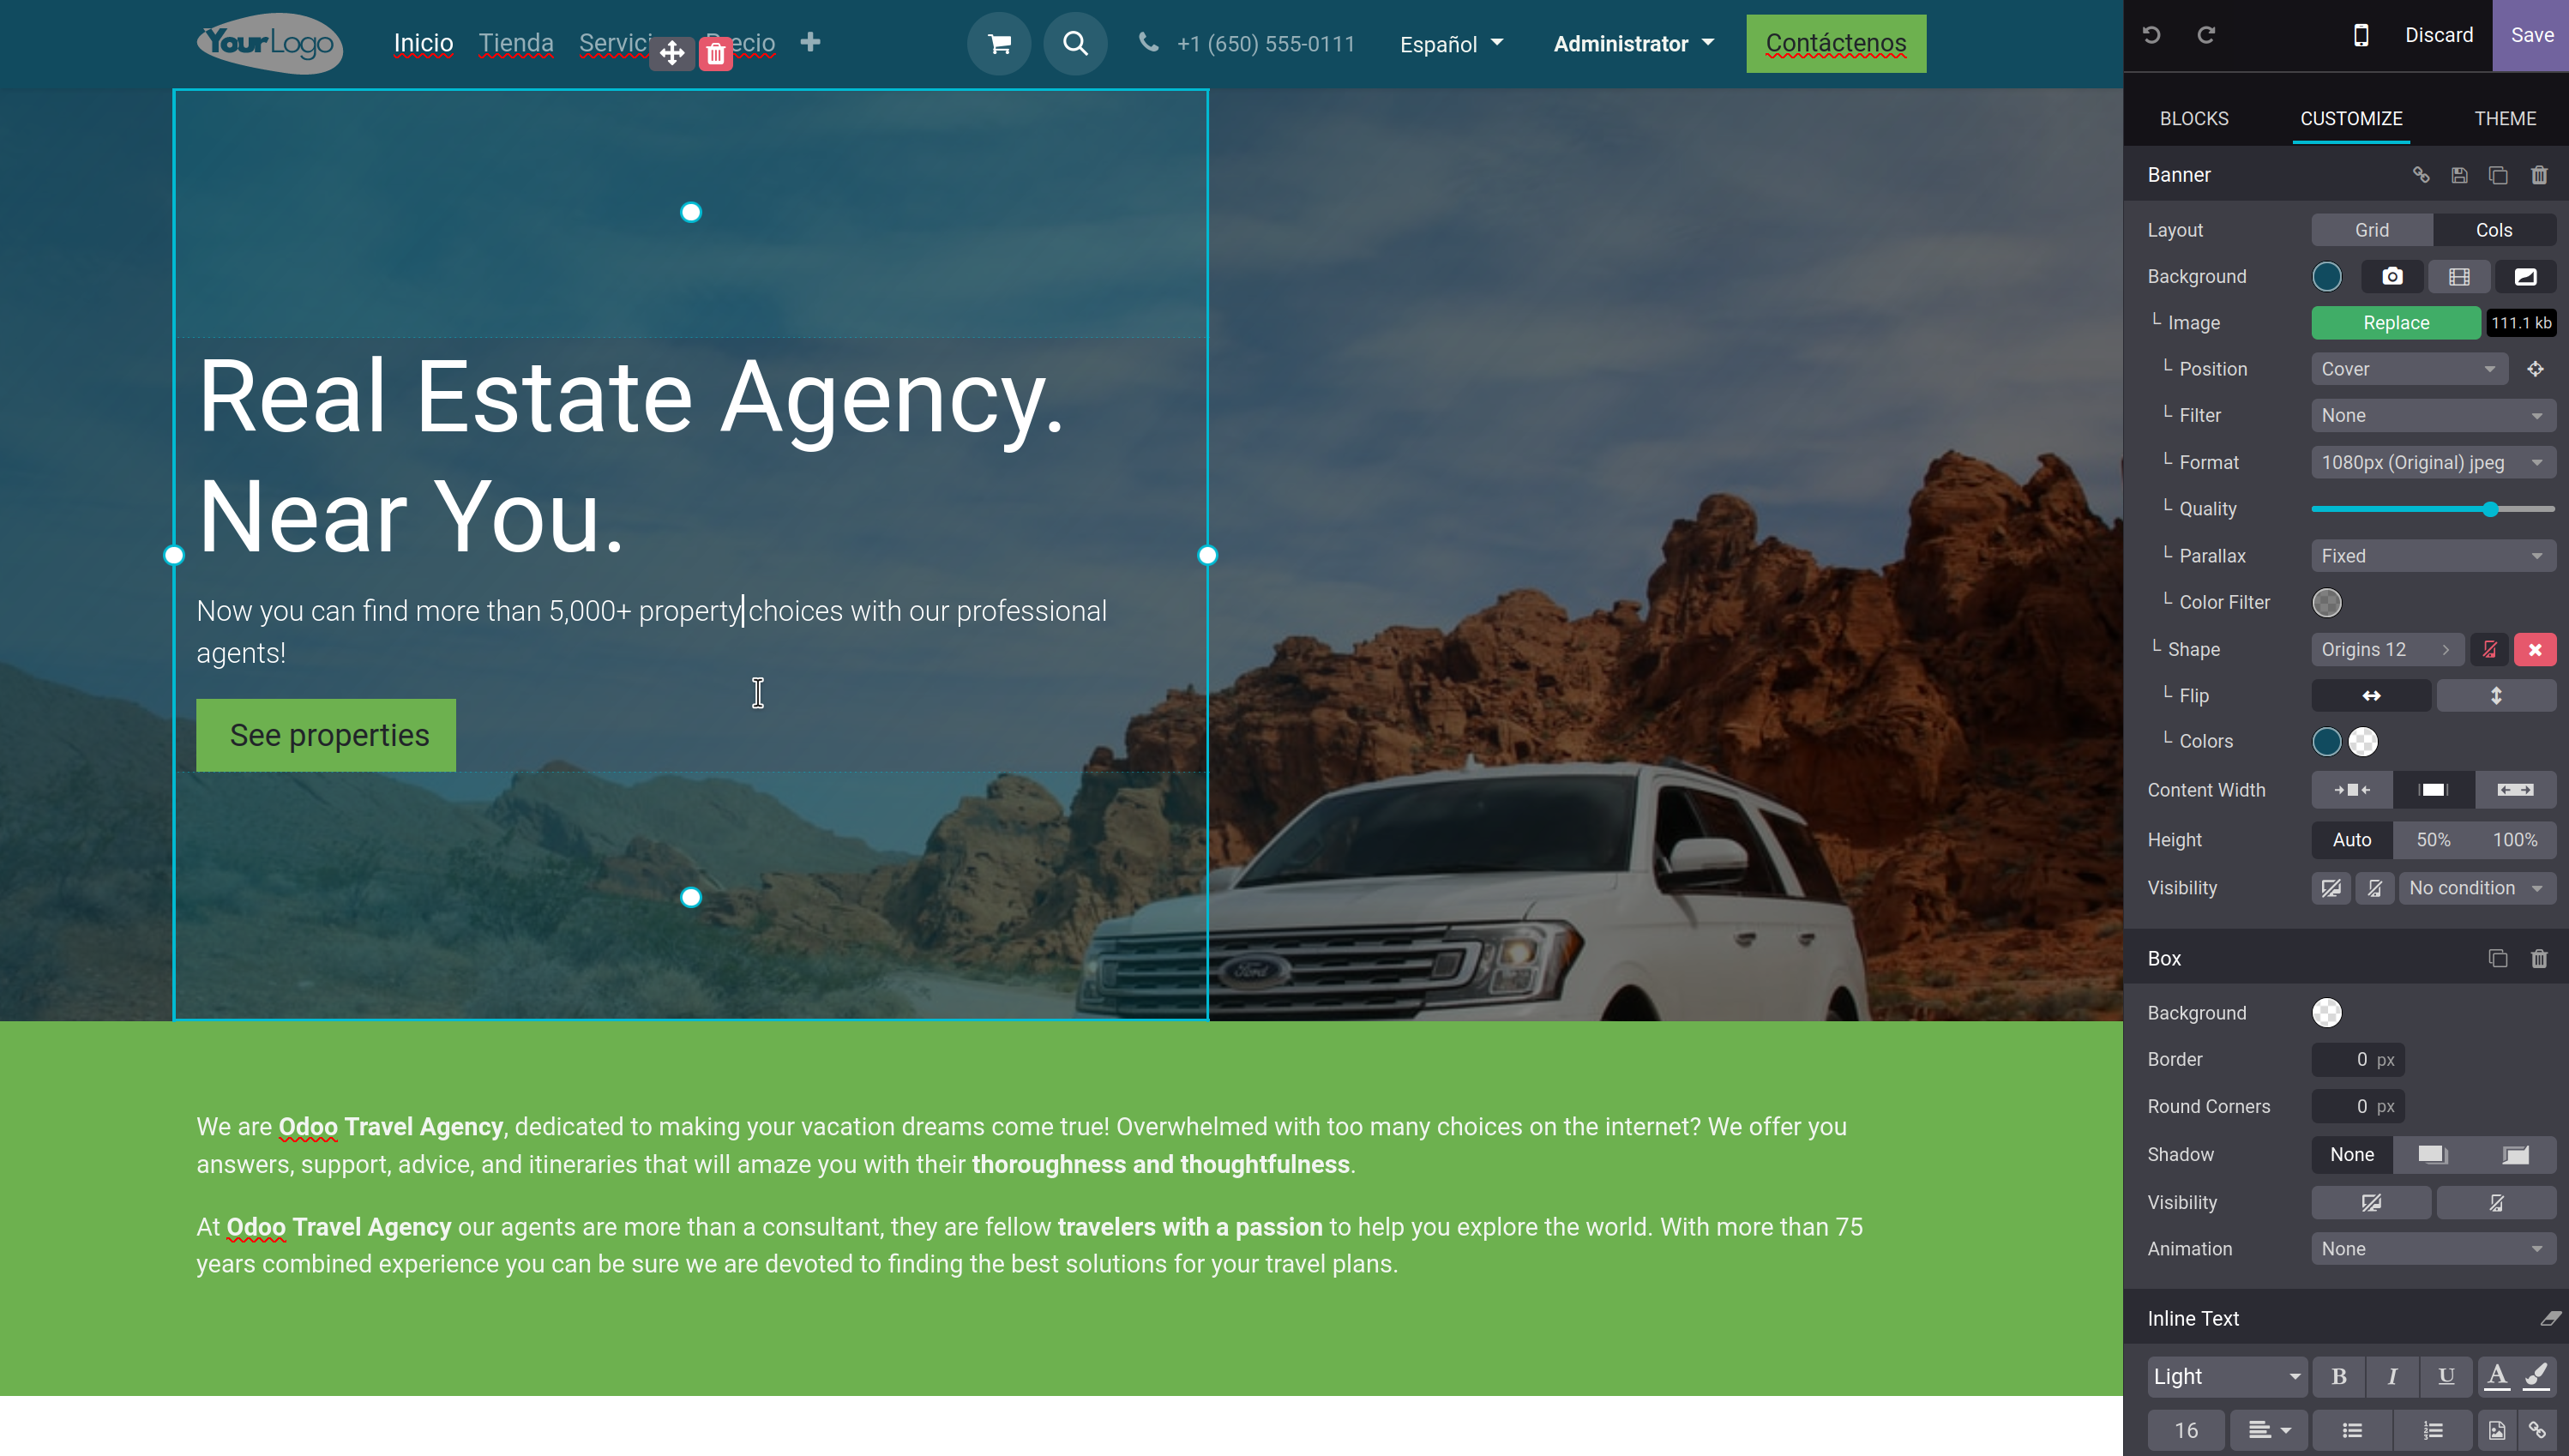
\includegraphics[width=6cm]{añadirInfoCompañia3.png}
    \caption{Edición de la misión de la compañía en la web.}
    \label{fig:faqs}
\end{figure}
\paragraph{}
Por otro lado, también se puede cambiar tanto los colores como el tema de la web.
Para cambiar el tema, se debe estar en el modo edición de la web y en el menú Tema en la barra lateral derecha de la siguiente manera.
\newpage
\begin{figure}[h]
    \centering
    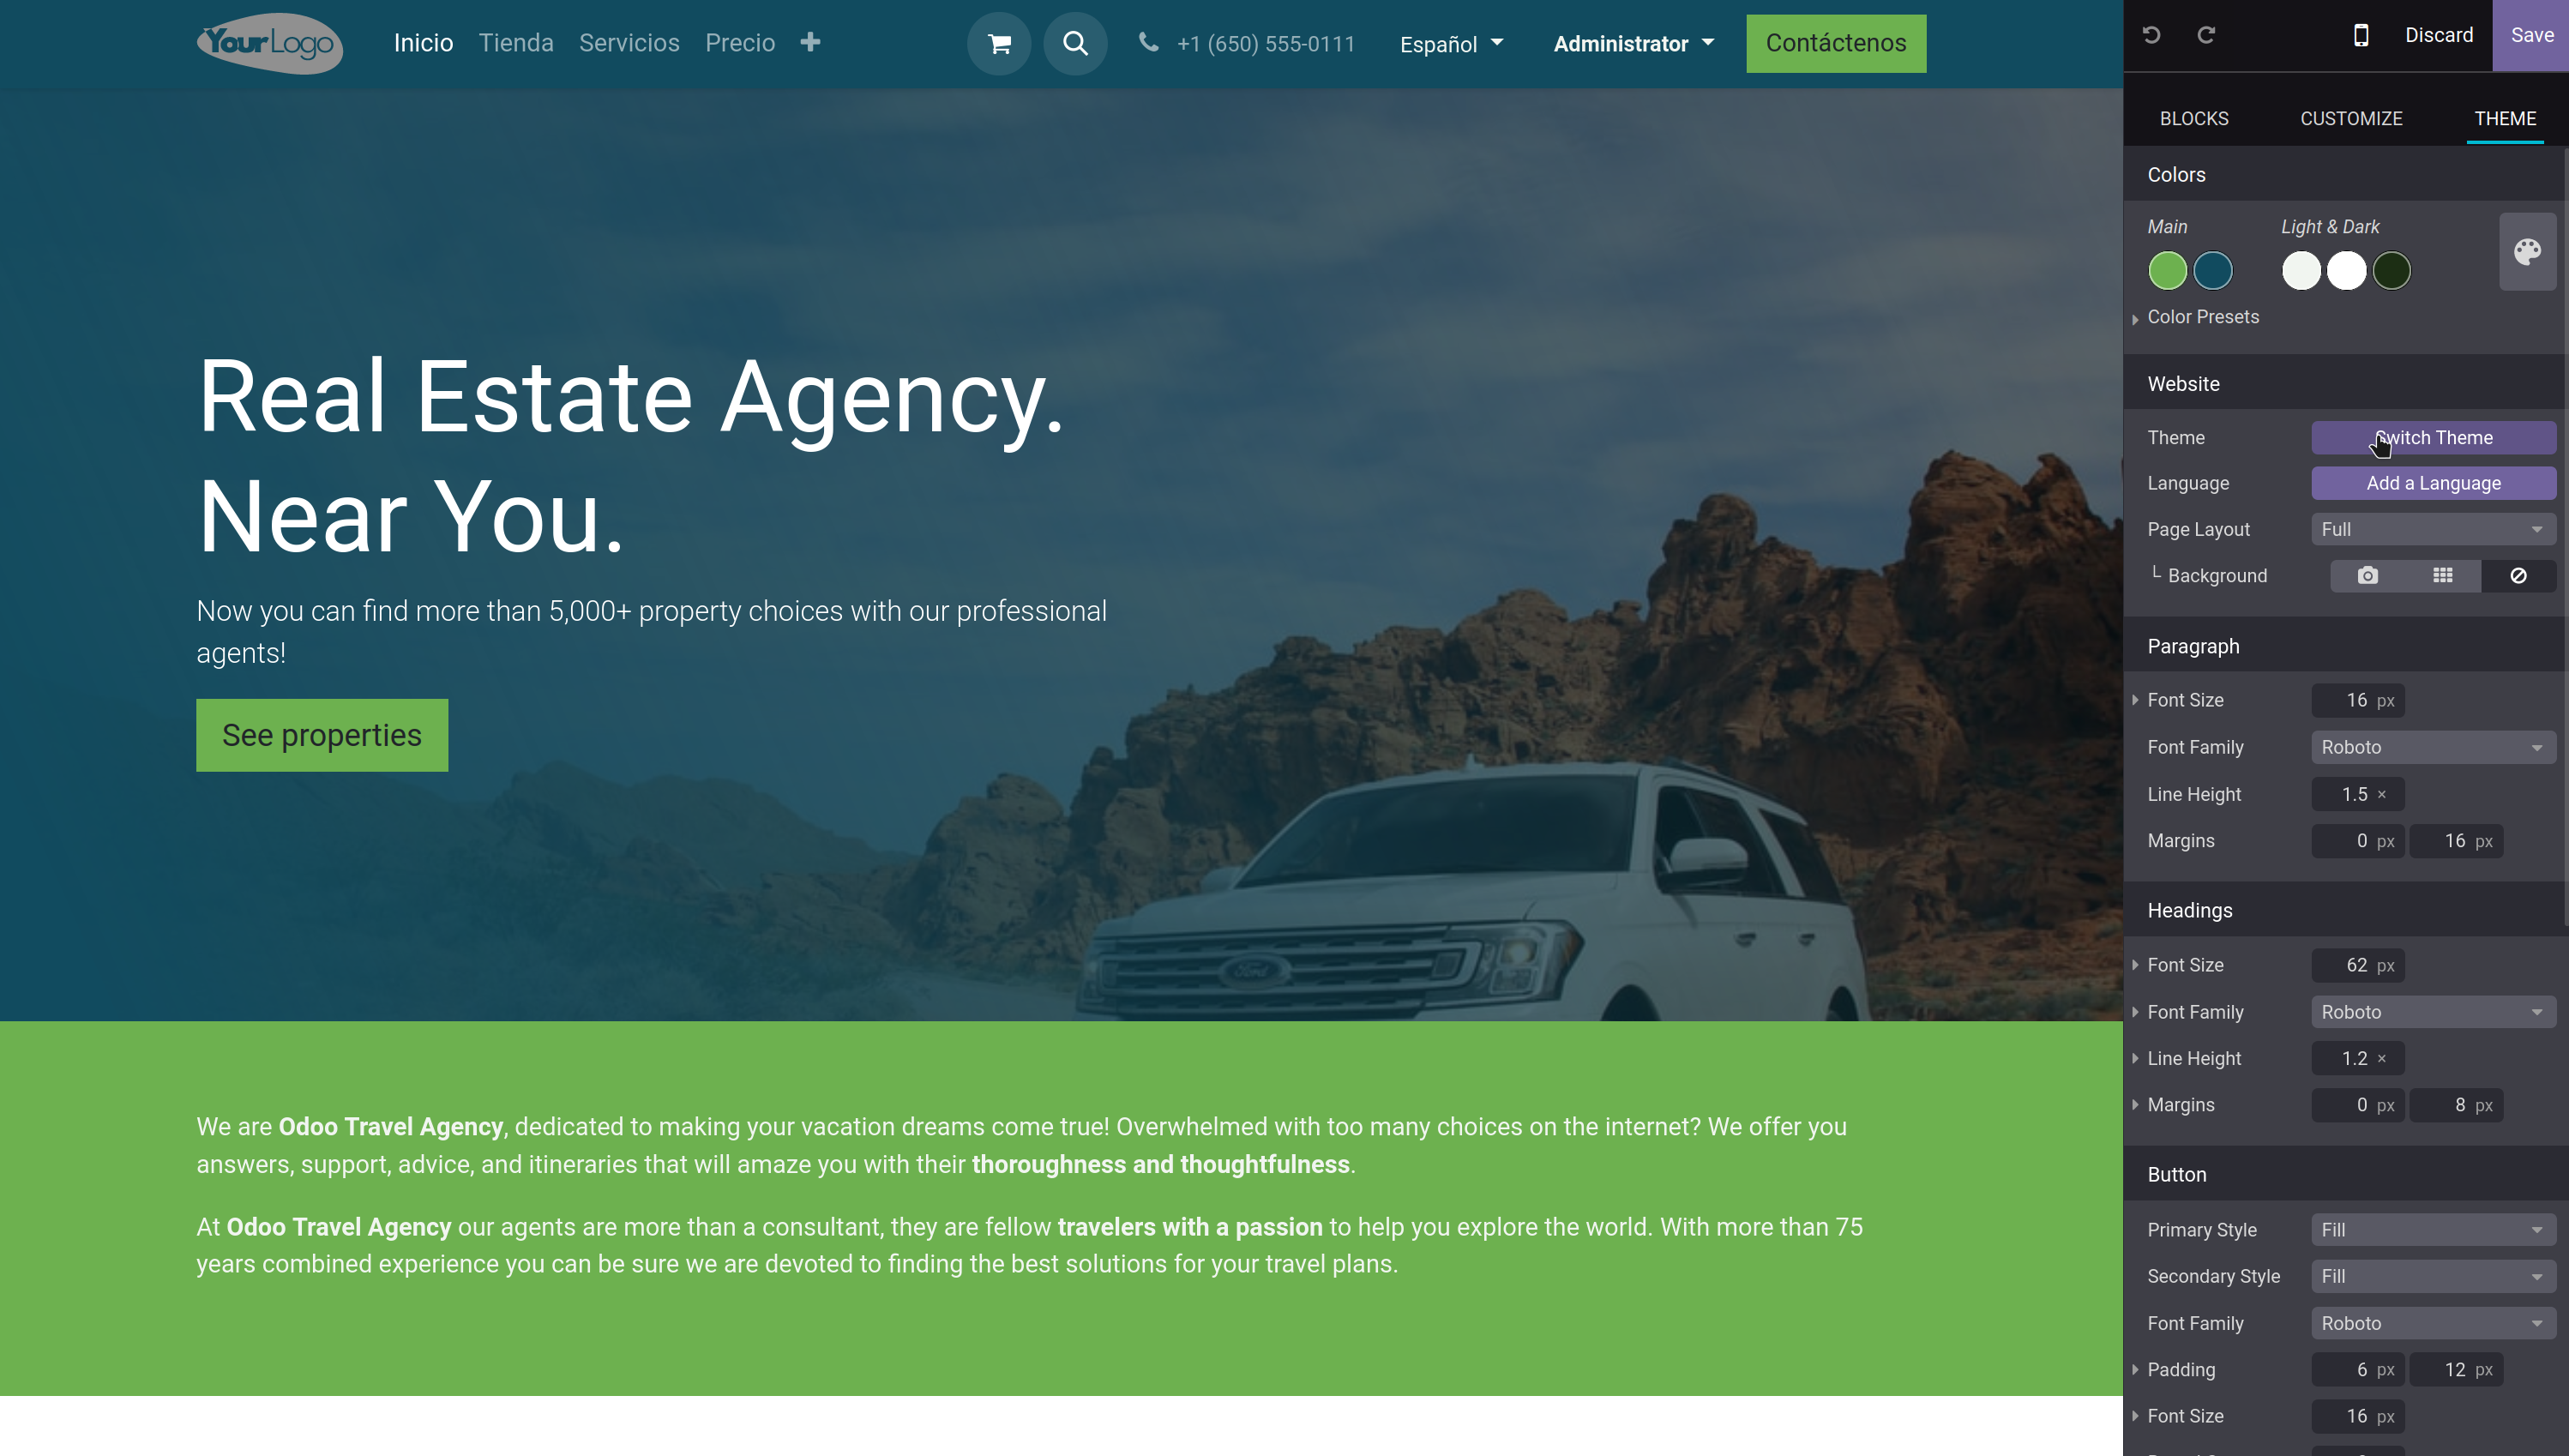
\includegraphics[width=6cm]{editTema.png}
    \caption{Personalización del tema de la web.}
    \label{fig:faqs}
\end{figure}
\paragraph{}
A continuación, se mostraran los temas disponibles y selecciona el que más se adapte a las necesidades de la compañía.
\begin{figure}[h]
    \centering
    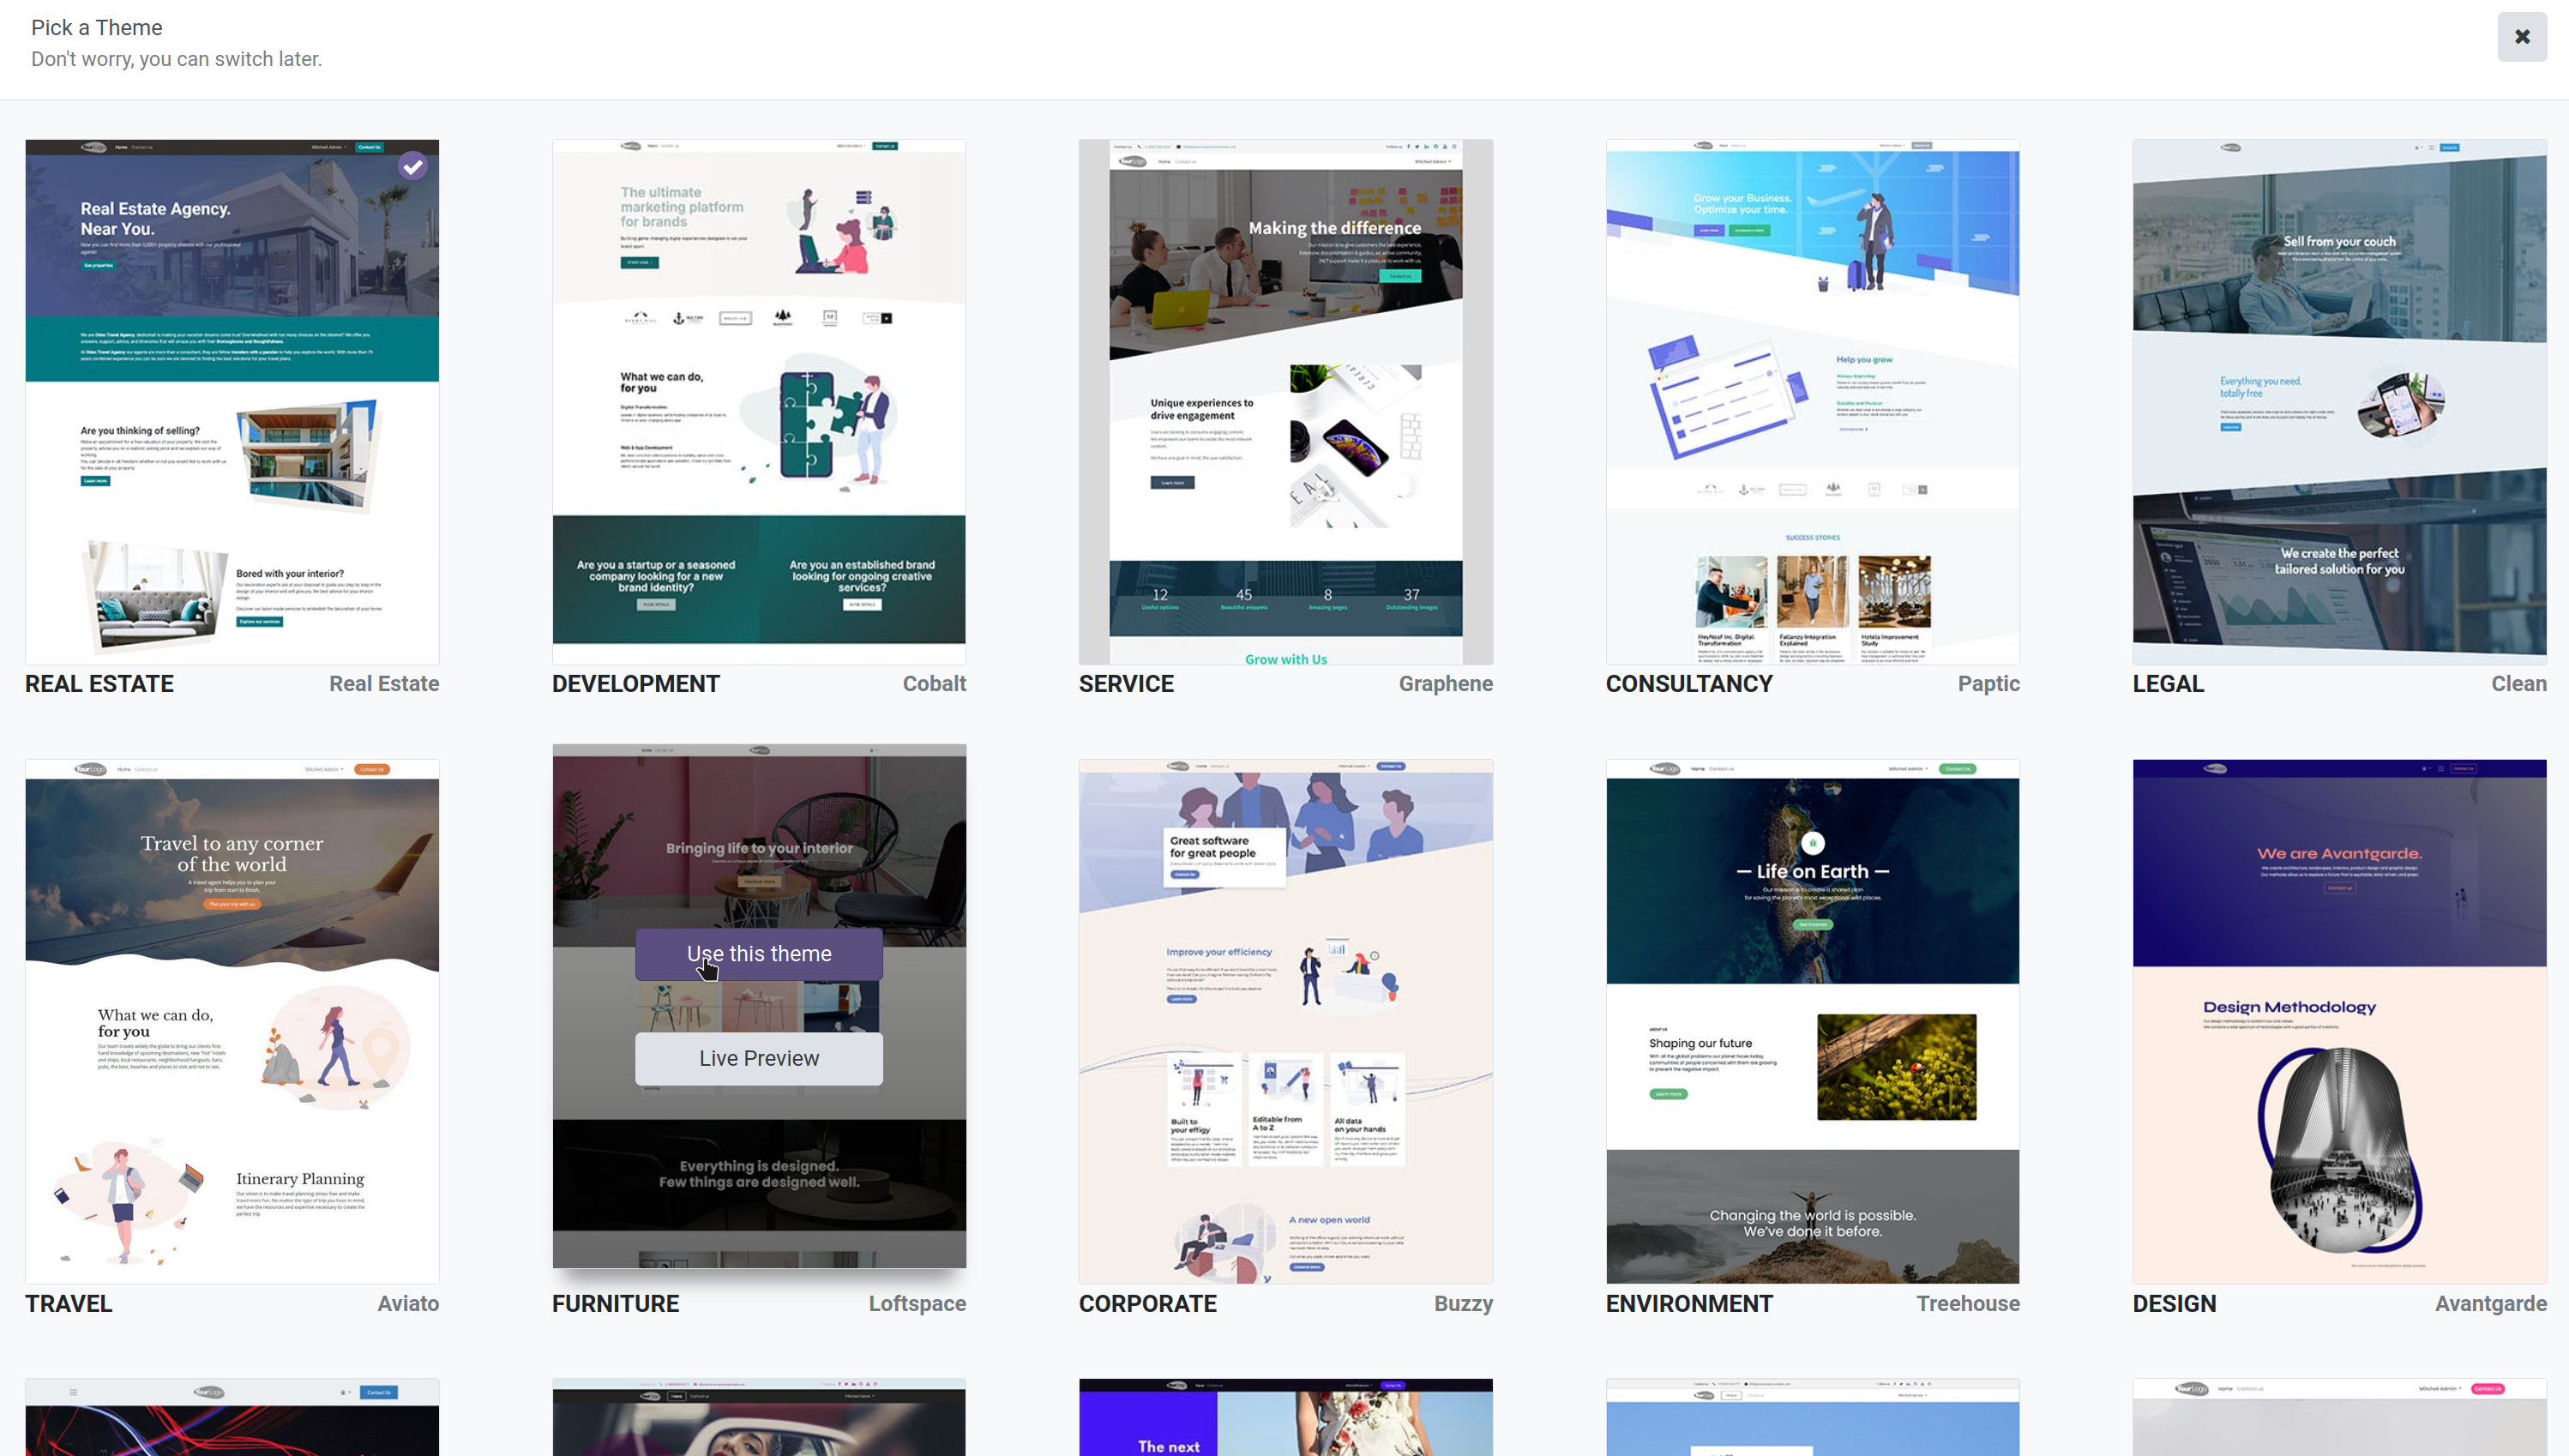
\includegraphics[width=6cm]{elegirTema.png}
    \caption{Elección del tema de la web.}
    \label{fig:faqs}
\end{figure}
\paragraph{}
Una vez, elegido el tema se puede personalizar el color de este. Para ello, en la parte superior del botón de cambiar el tema se encuentra las opciones de color. Si se hace click encima de un color se puede cambiar por otro que se eliga, sino se pueden elegir entre unos colores ya predefinidos haciendo click en la paleta de colores.
\begin{figure}[h]
    \centering
    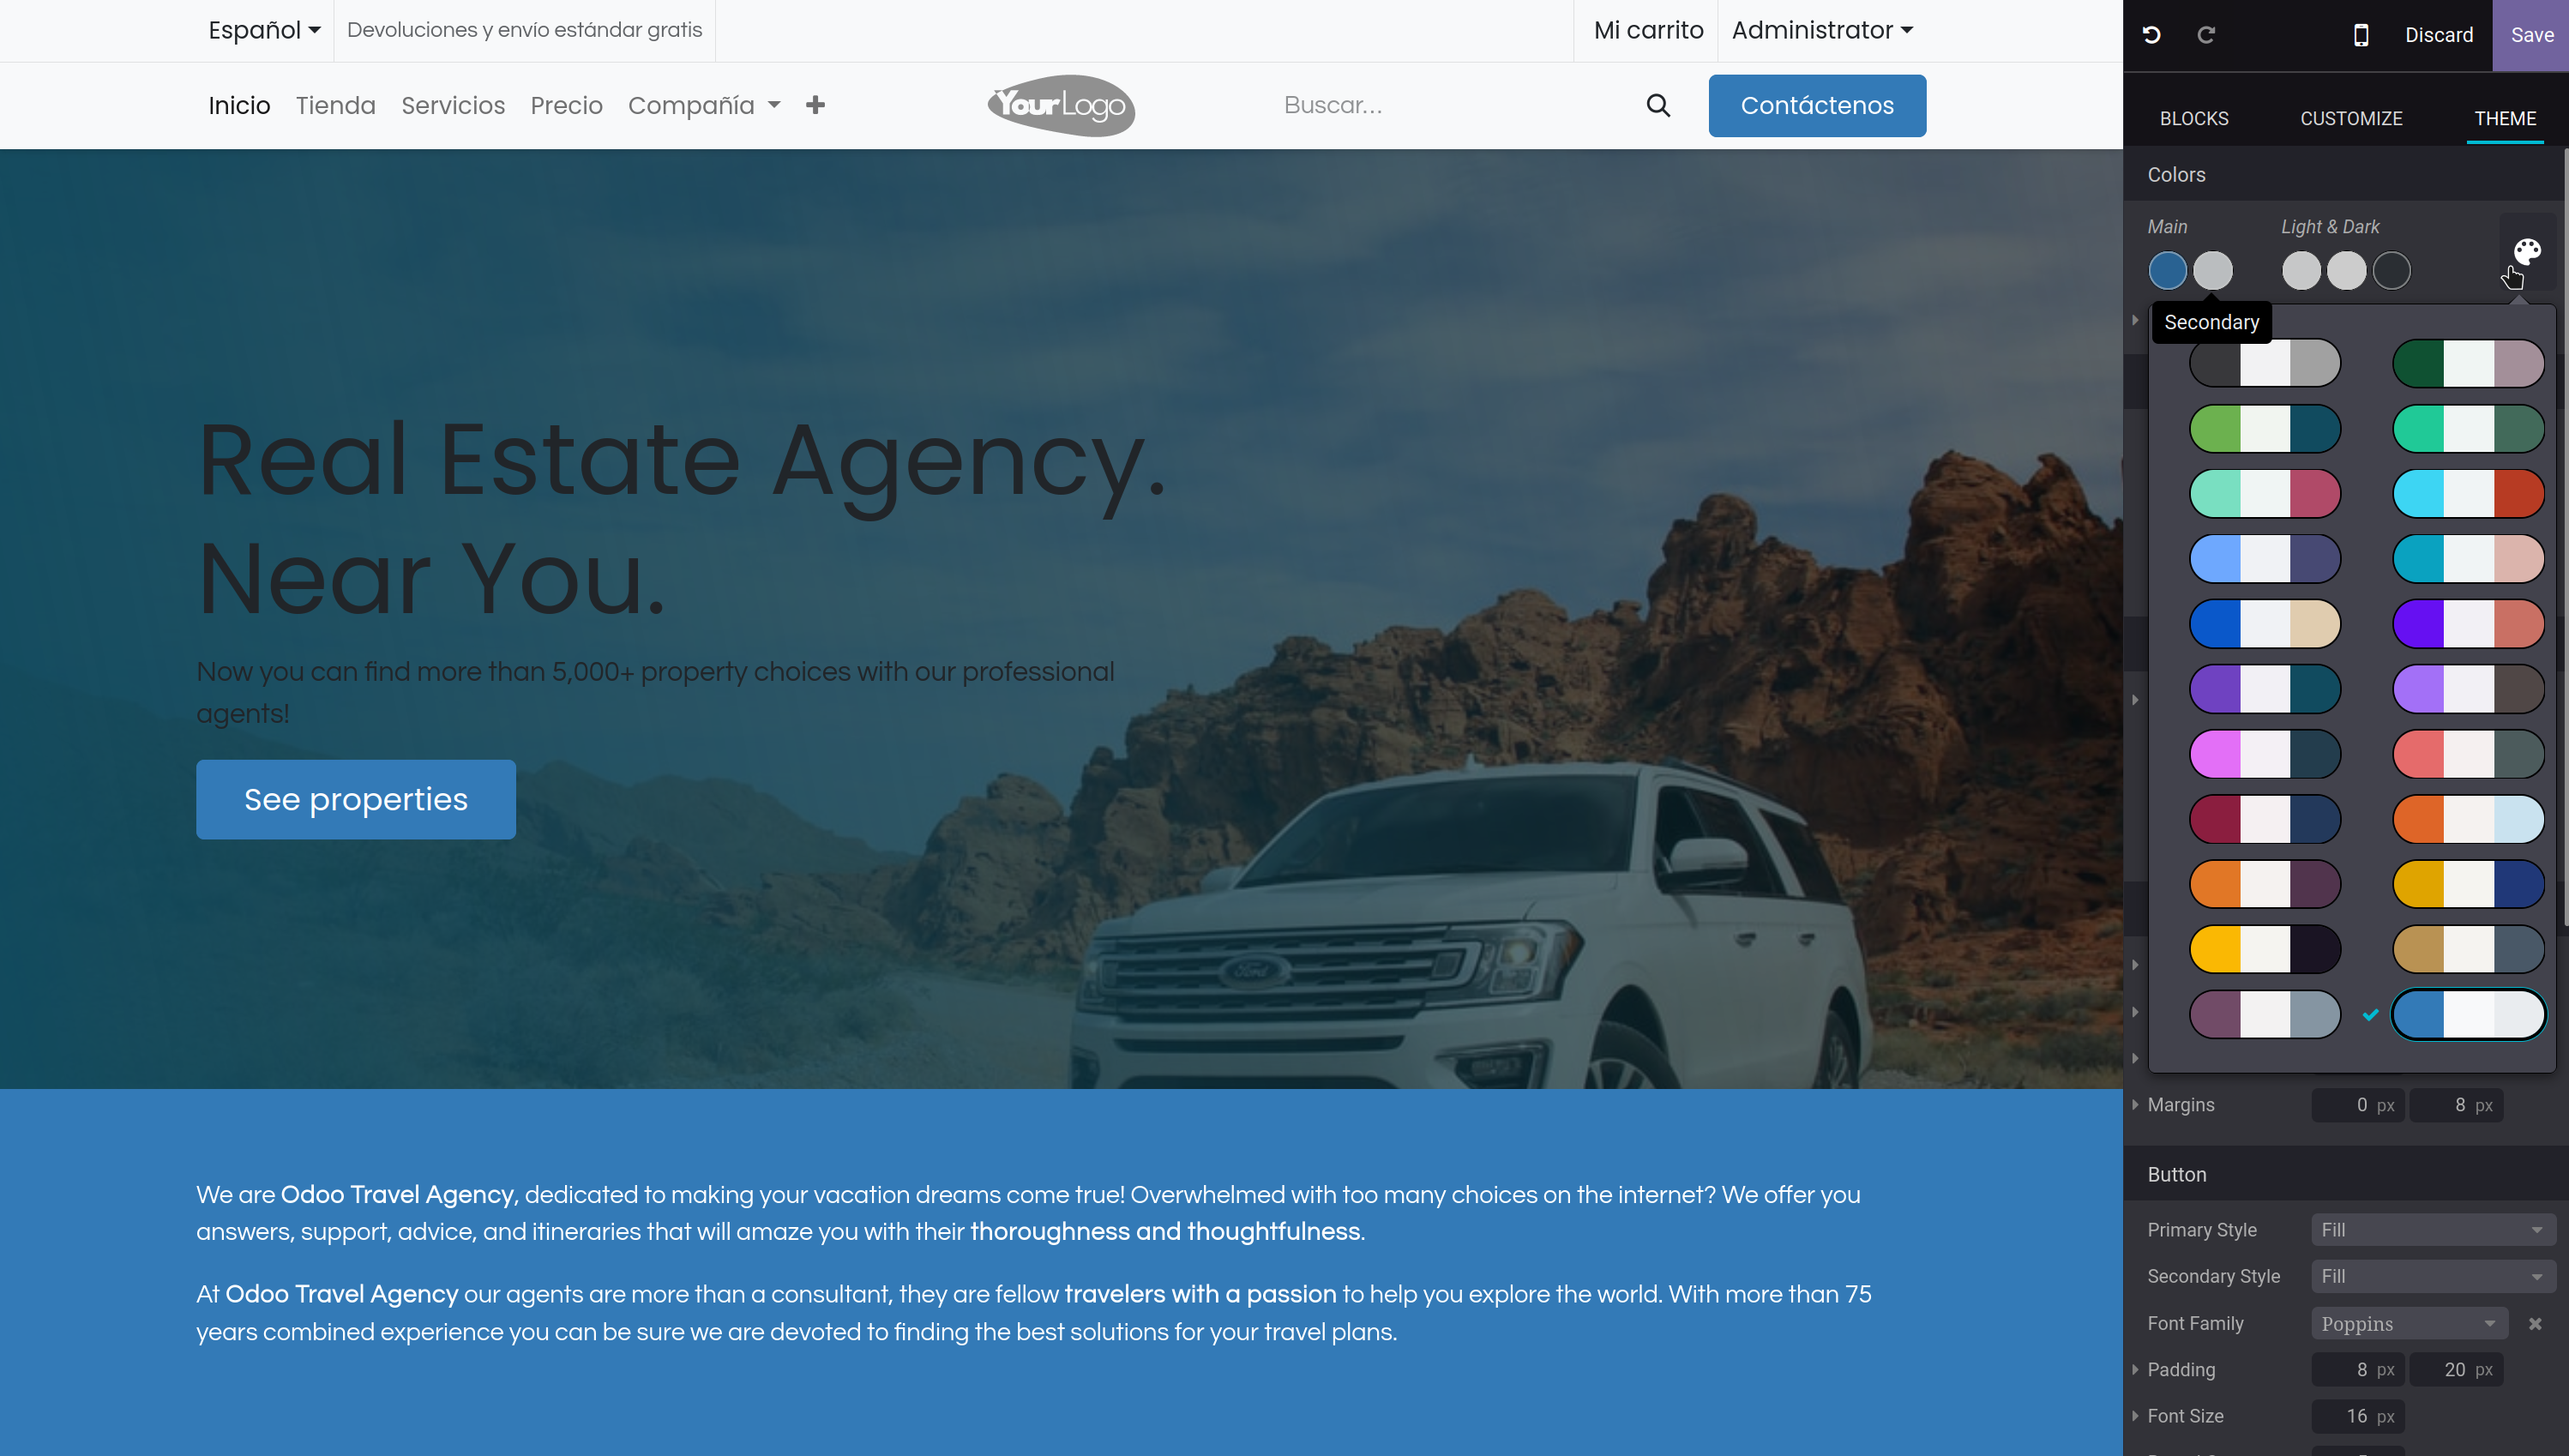
\includegraphics[width=6cm]{cambiarColor.png}
    \caption{Personalización del color del tema de la web.}
    \label{fig:faqs}
\end{figure}
\paragraph{}
Si se quiere añadir el logo a la página web, se debe estar en el modo edición en la pagina web. Haz doble click en el logo predefinido. Selecciona la opción de subir una imagen. A continuación, busca y selecciona la imagen del logo que se encuentra en tu máquina. Te aparecerá entre las imagenes para escoger, haz click en ella para convertirla en tu logo.
\newpage
\begin{figure}[h]
    \centering
    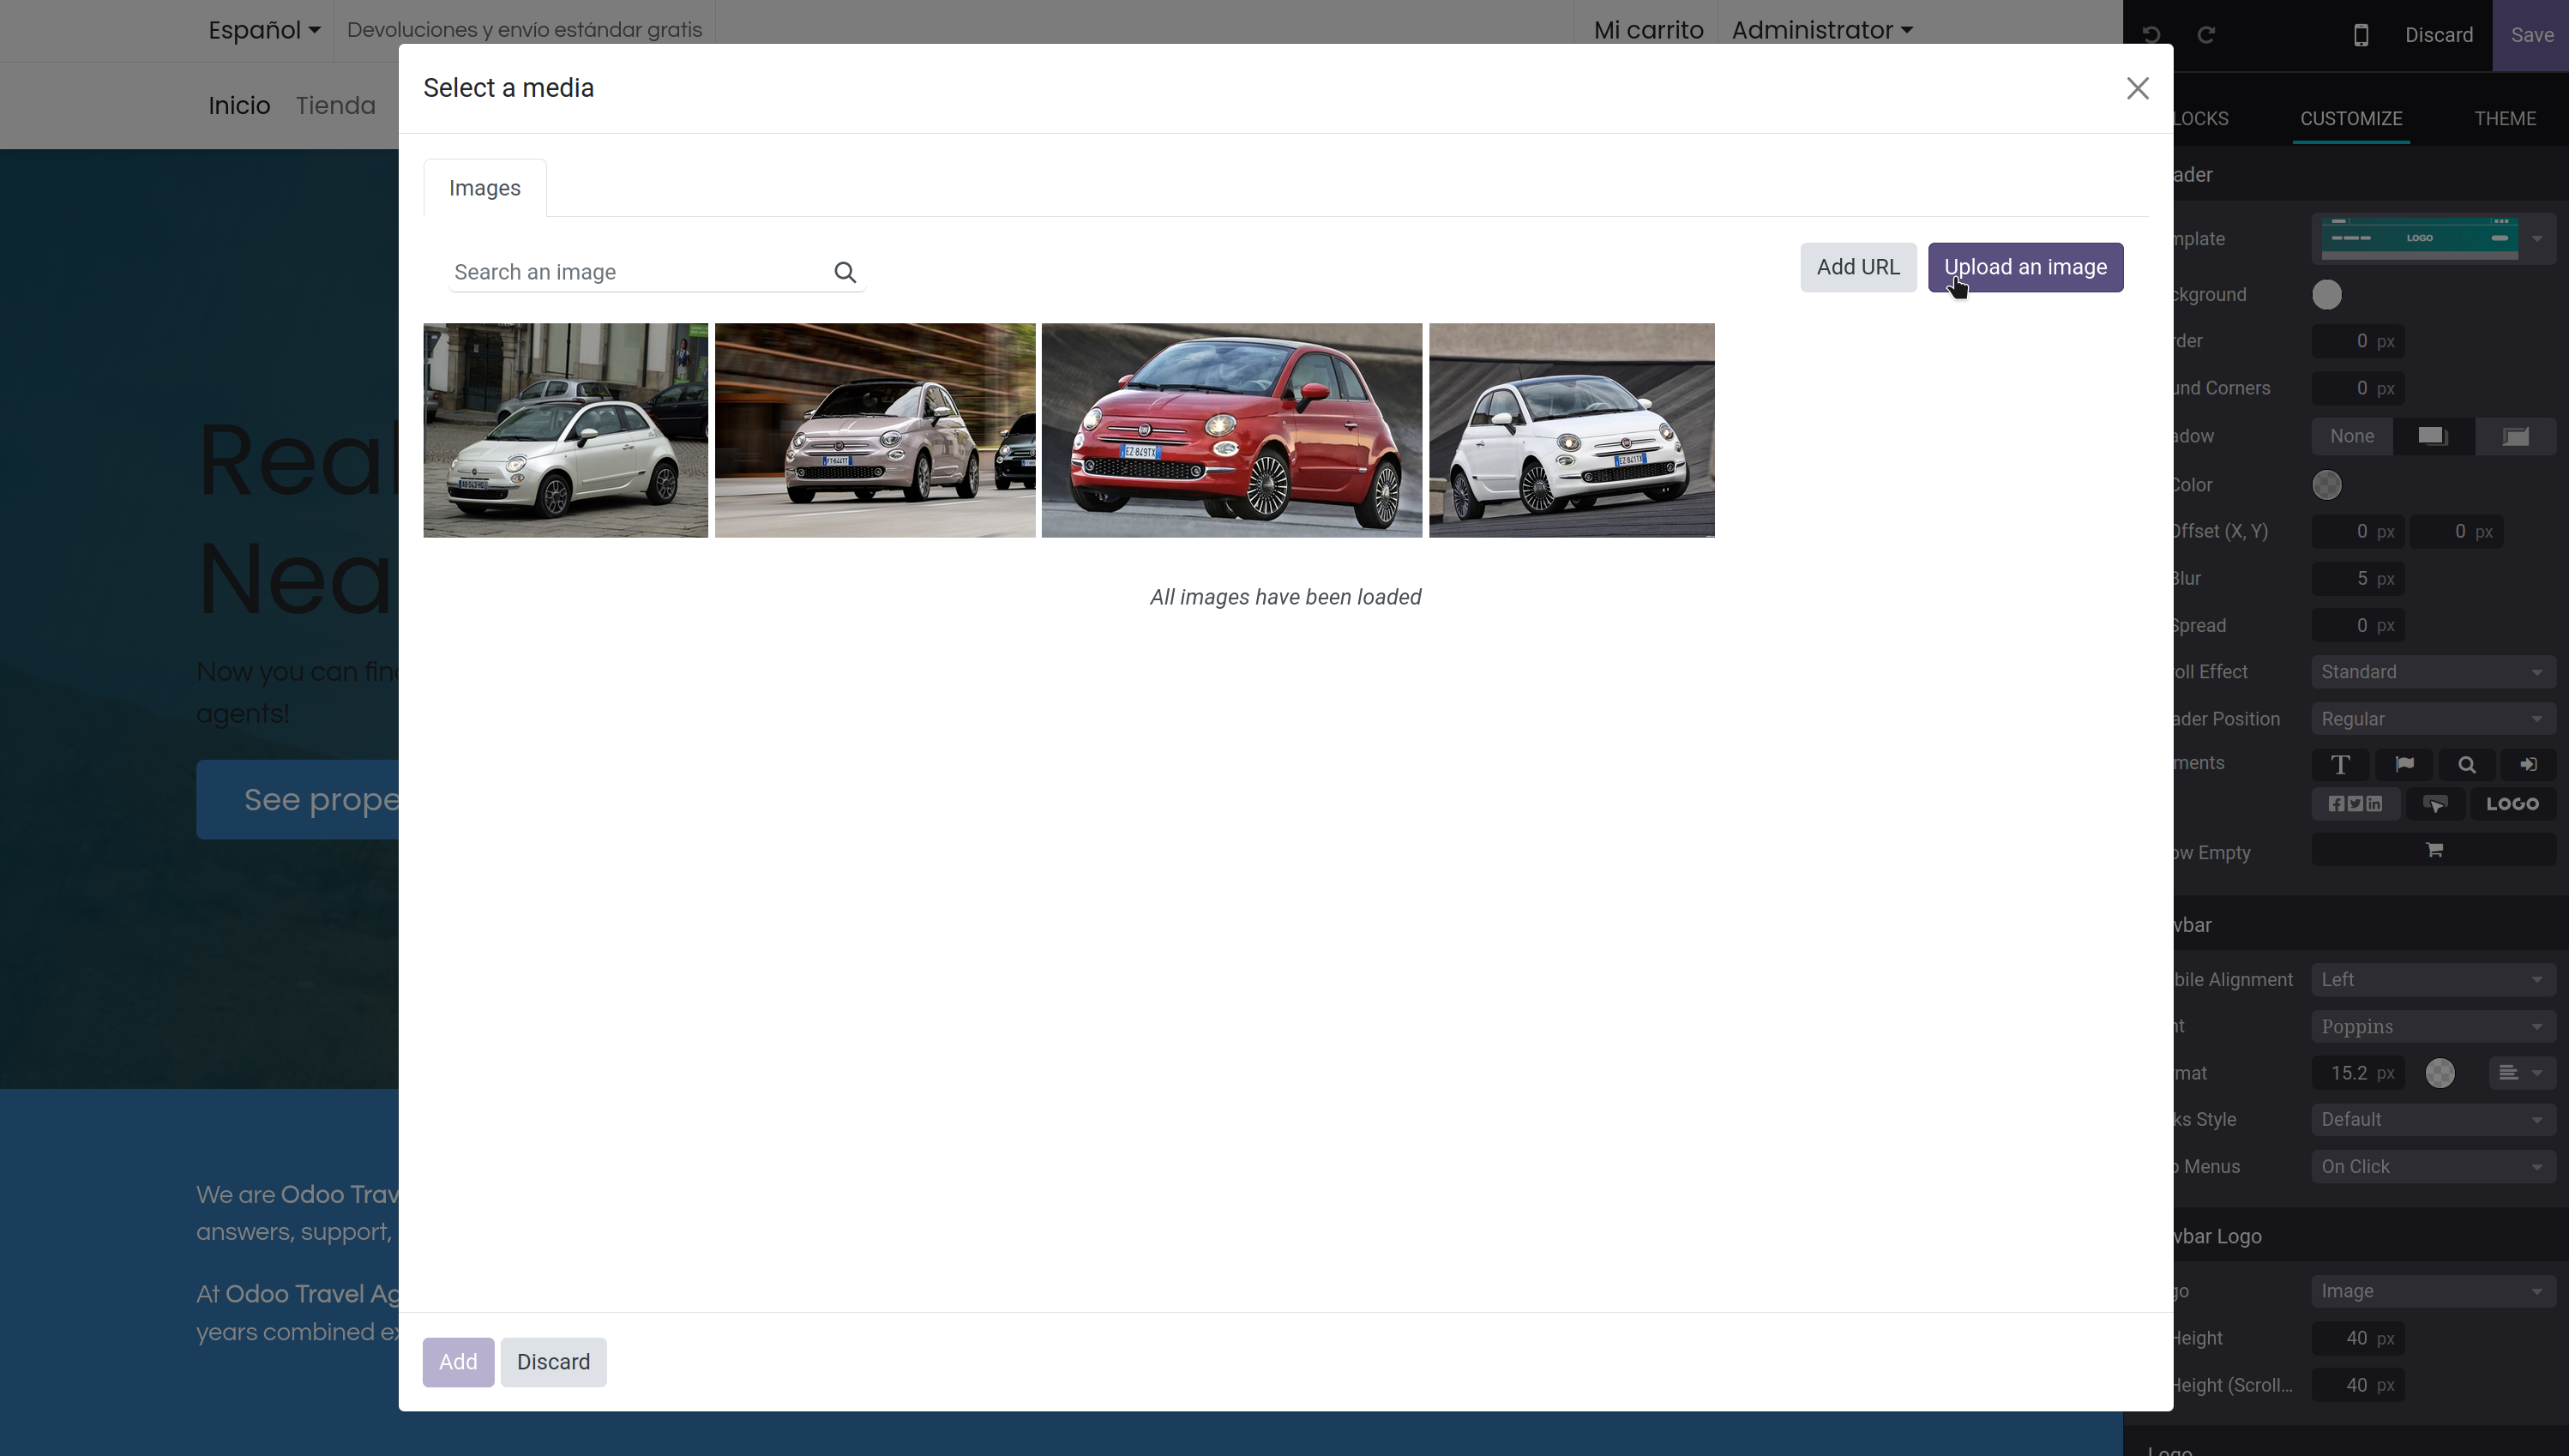
\includegraphics[width=6cm]{añadirLogo.png}
    \caption{Personalización del logo.}
    \label{fig:faqs}
\end{figure}
\paragraph{}
Para realizar una configuración para mejorar en el ranking de búsqueda de Google, se debe ir al menú de configuración de la web y seleccionar la opción de SEO.
En este menú se pueden editar el titulo y la descripción que aparecerá desde el buscador de Google y se puede añadir una imagen que se mostrará en el buscador de Google.
Además, se encuentra la configuración de las palabras clave de Google, que son las palabras que se quieren que se asocien a la web. Para añadir una palabra clave se debe introducir el termino y el idioma de este y hacer click en la opción de Añadir .
En la lista de la parte inferior aparece información de la palabra, en que tipos de ubicaciones se encuentra en la web y otras palabras relacionadas.
\begin{figure}[h]
    \centering
    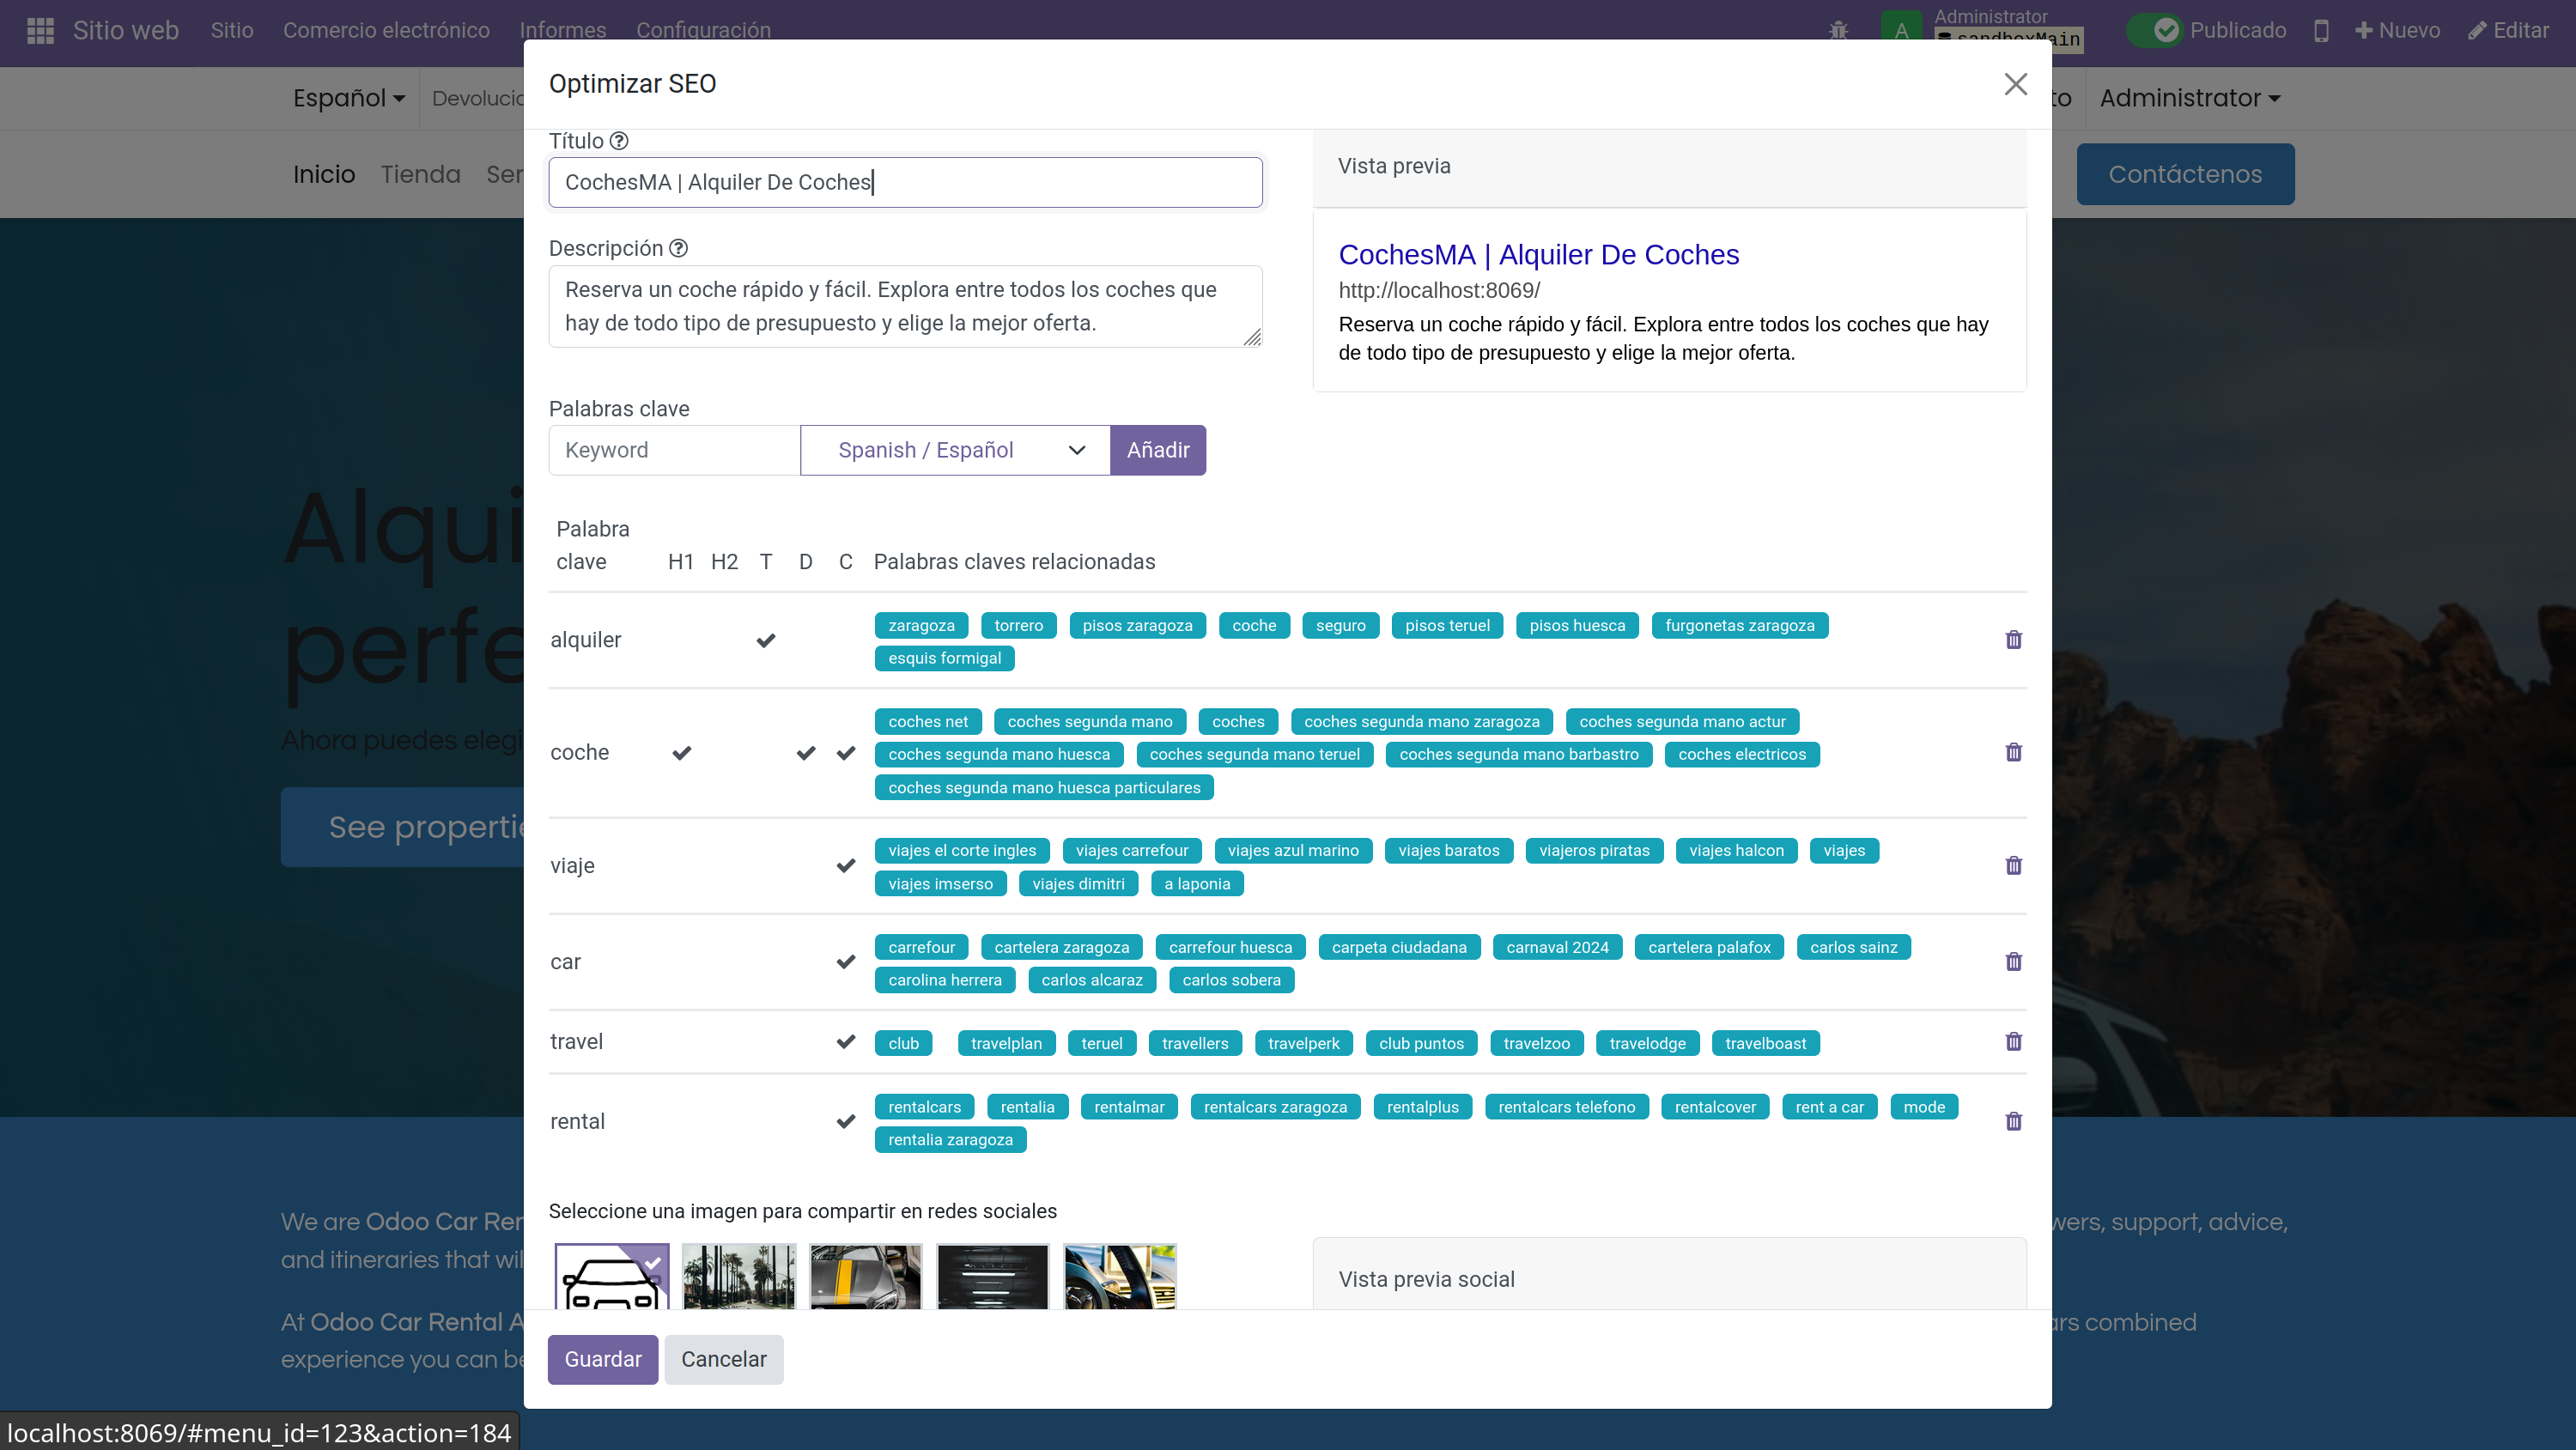
\includegraphics[width=6cm]{rankingGoogle.png}
    \caption{Configuración de optimicaziones SEO.}
    \label{fig:faqs}
\end{figure}
\section{Configuración técnica}
\paragraph{}
Odoo ofrece una interfaz para gestionar las bases de datos que se encuentran en la máquina. Para acceder a este menú dirigese al enlace: https://localhost:8069/web/database/manager.
\begin{figure}[h]
    \centering
    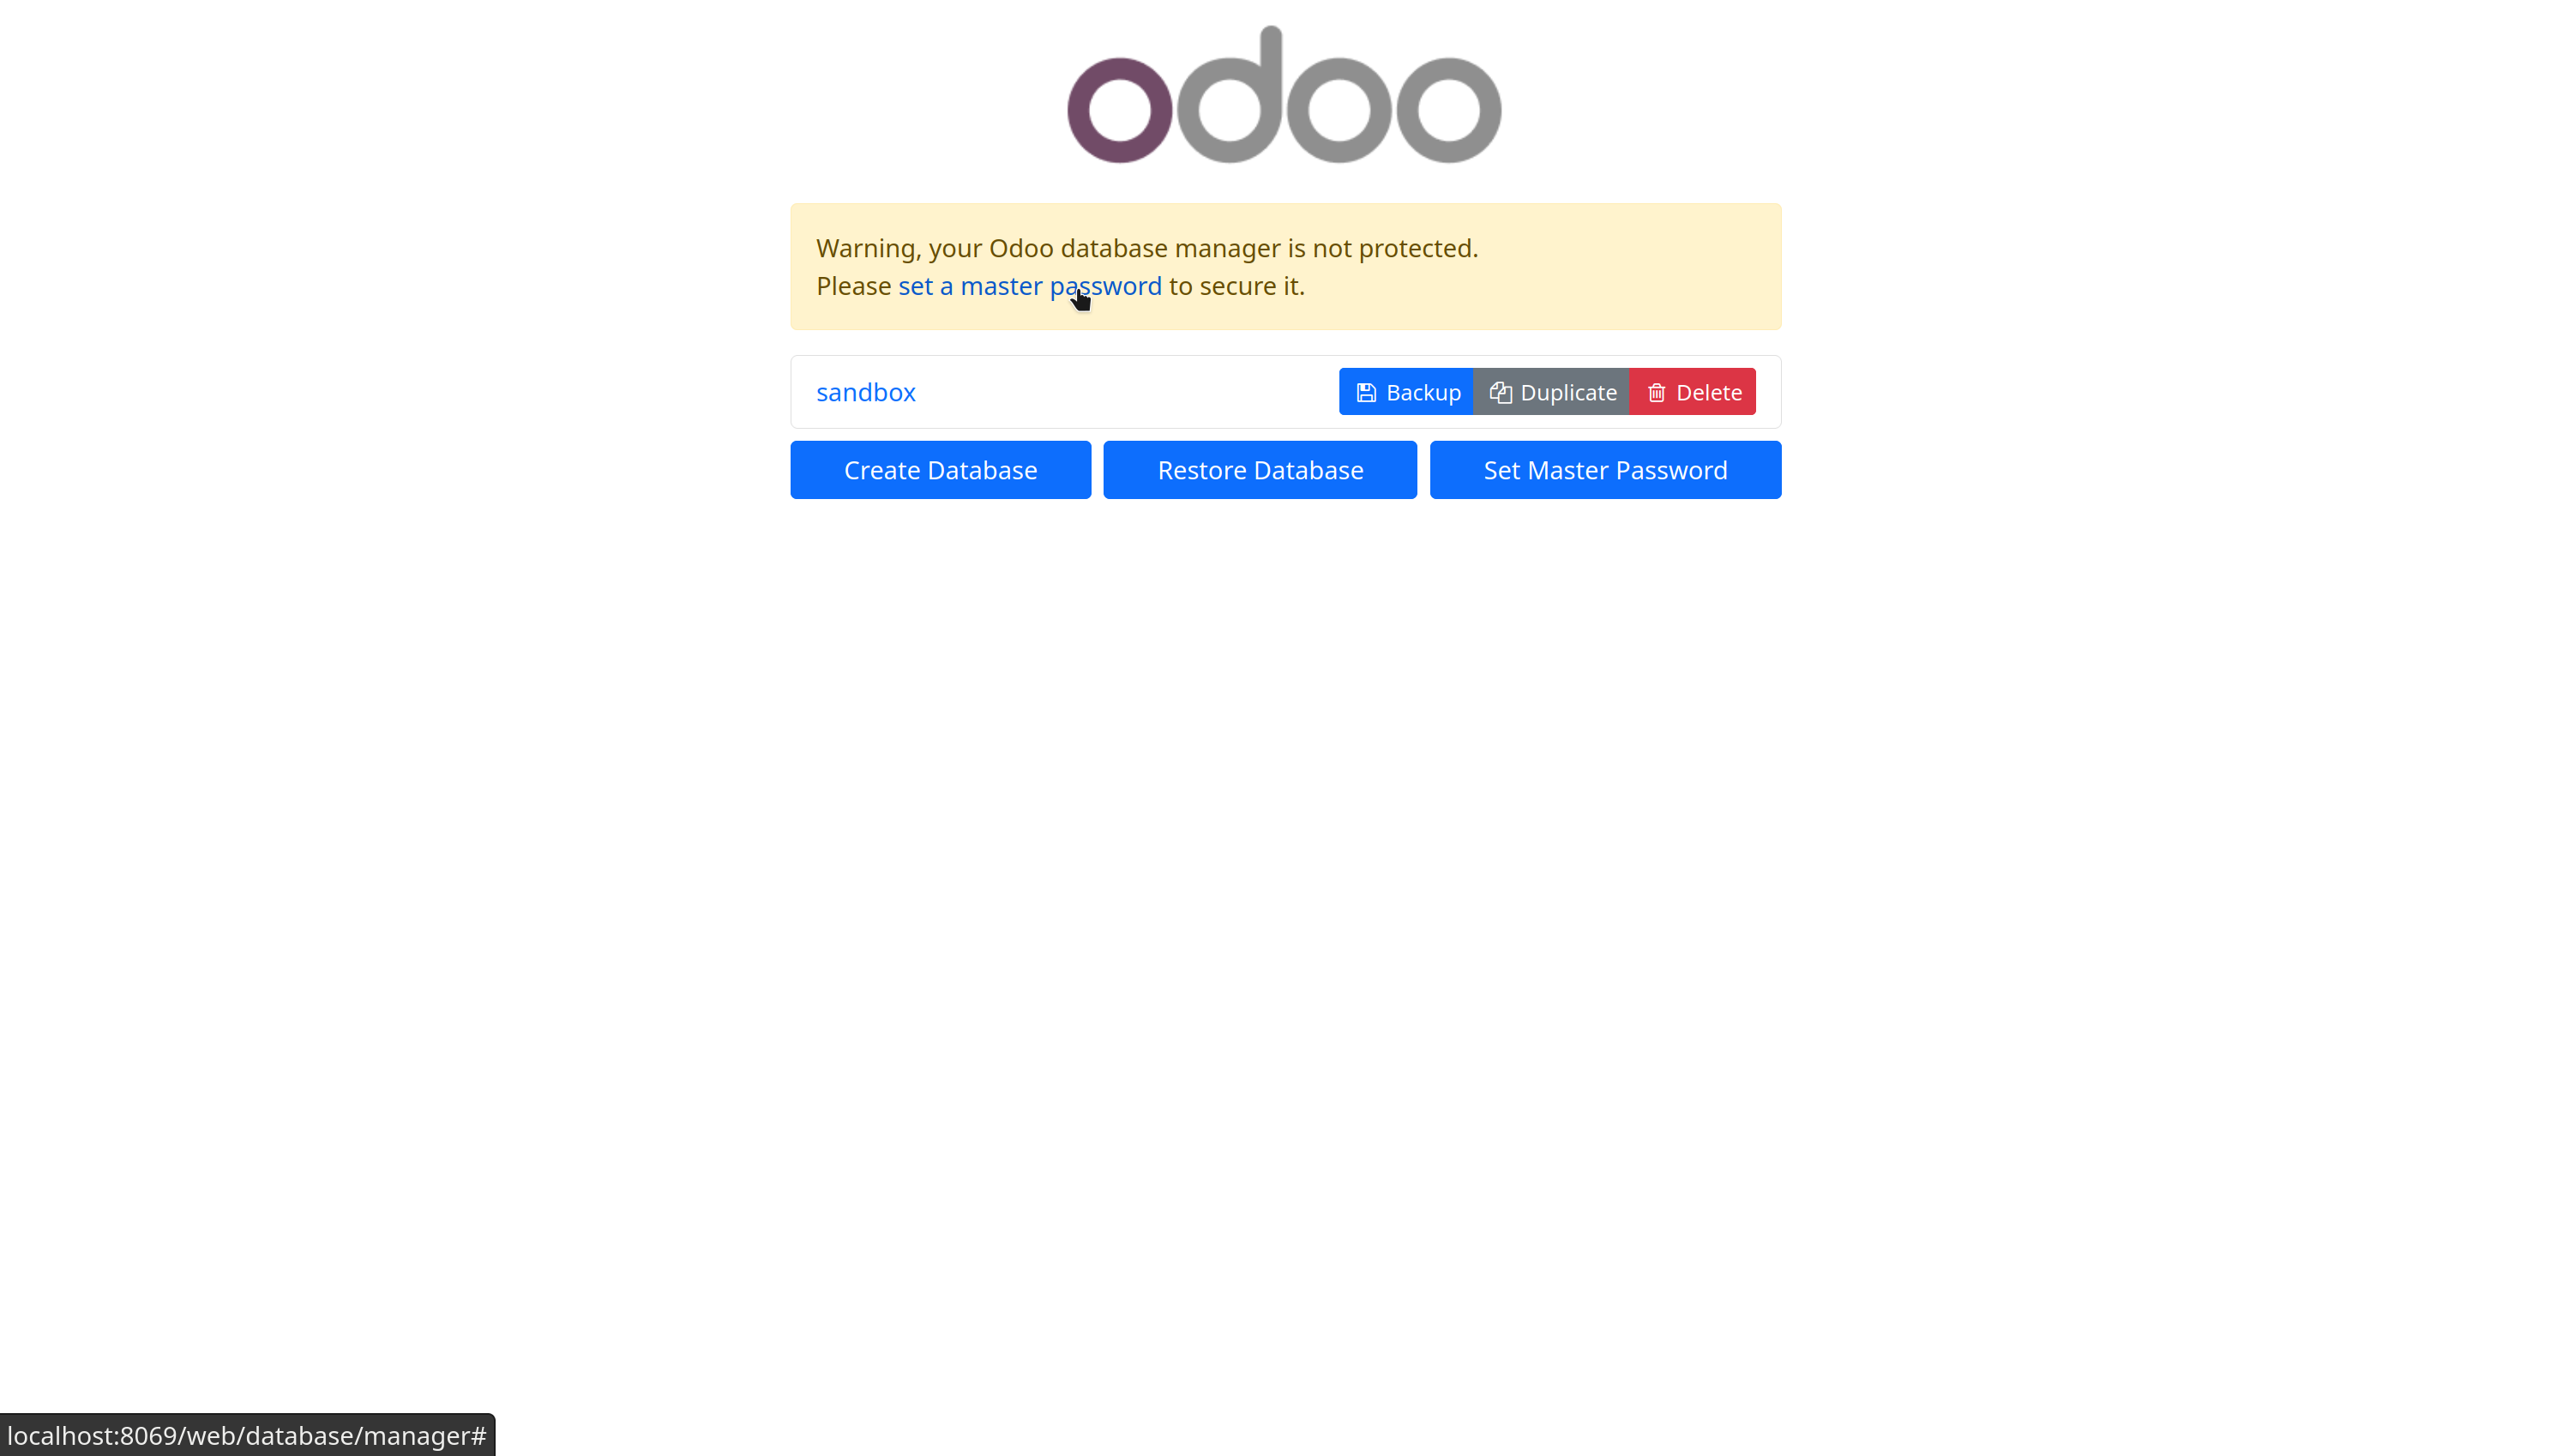
\includegraphics[width=6cm]{manageDb.png}
    \caption{Menú de gestión de bases de datos.}
    \label{fig:faqs}
\end{figure}
\paragraph{}
Primero, haz click en Set a master password, introduce la nueva contraseña maestra y pulsa en Continue. 
Odoo ofrece una opción para crear una nueva base de datos, para ello haz click en Create Database. Introduce la información correspondiente y pulsa en Continue.
\newpage
\begin{figure}[h]
    \centering
    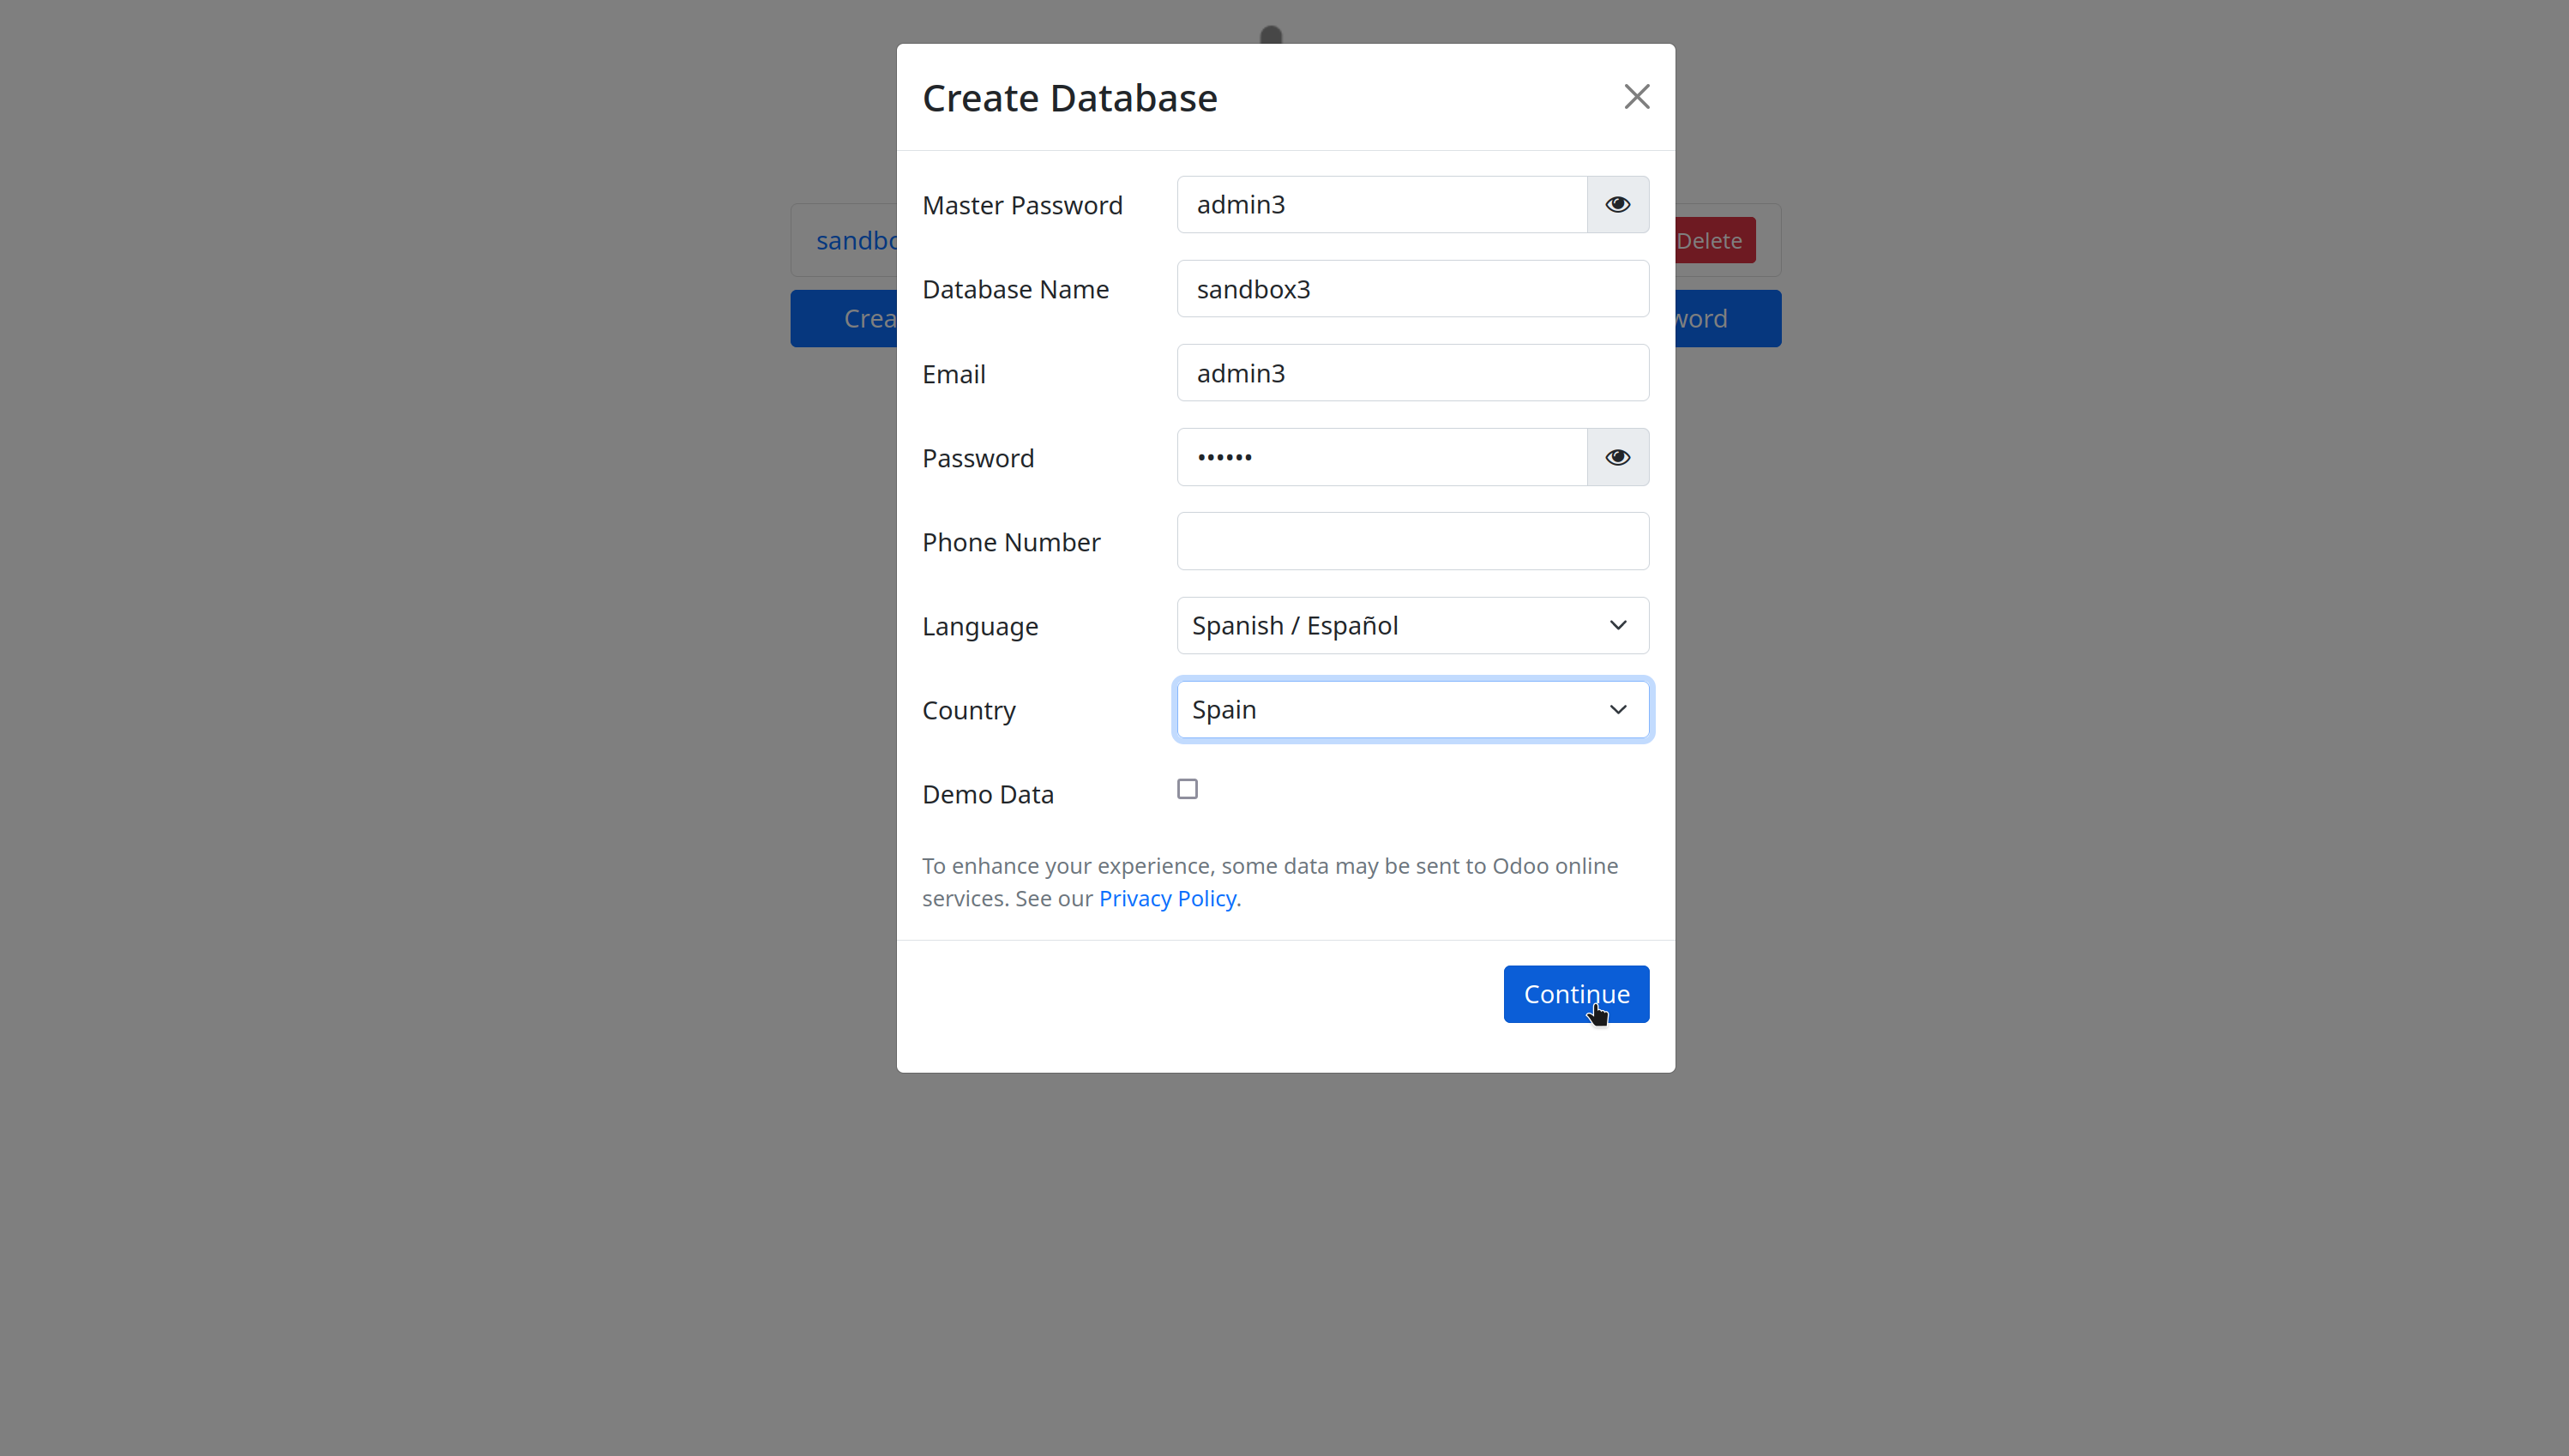
\includegraphics[width=6cm]{crearDb.png}
    \caption{Creación de una base de datos.}
    \label{fig:faqs}
\end{figure}
\paragraph{}
Una vez creada, inicia sesión con la información introducida anteriormente y se accederá al menú de aplicaciones como se ha explicado en la sección de instalación.
Odoo ofrece la posibilidad de duplicar una base de datos. Selecciona la opción Duplicate de la base de datos a duplicar. Introduce la información de la siguiente imagen y pulsa en Continue.
\begin{figure}[h]
    \centering
    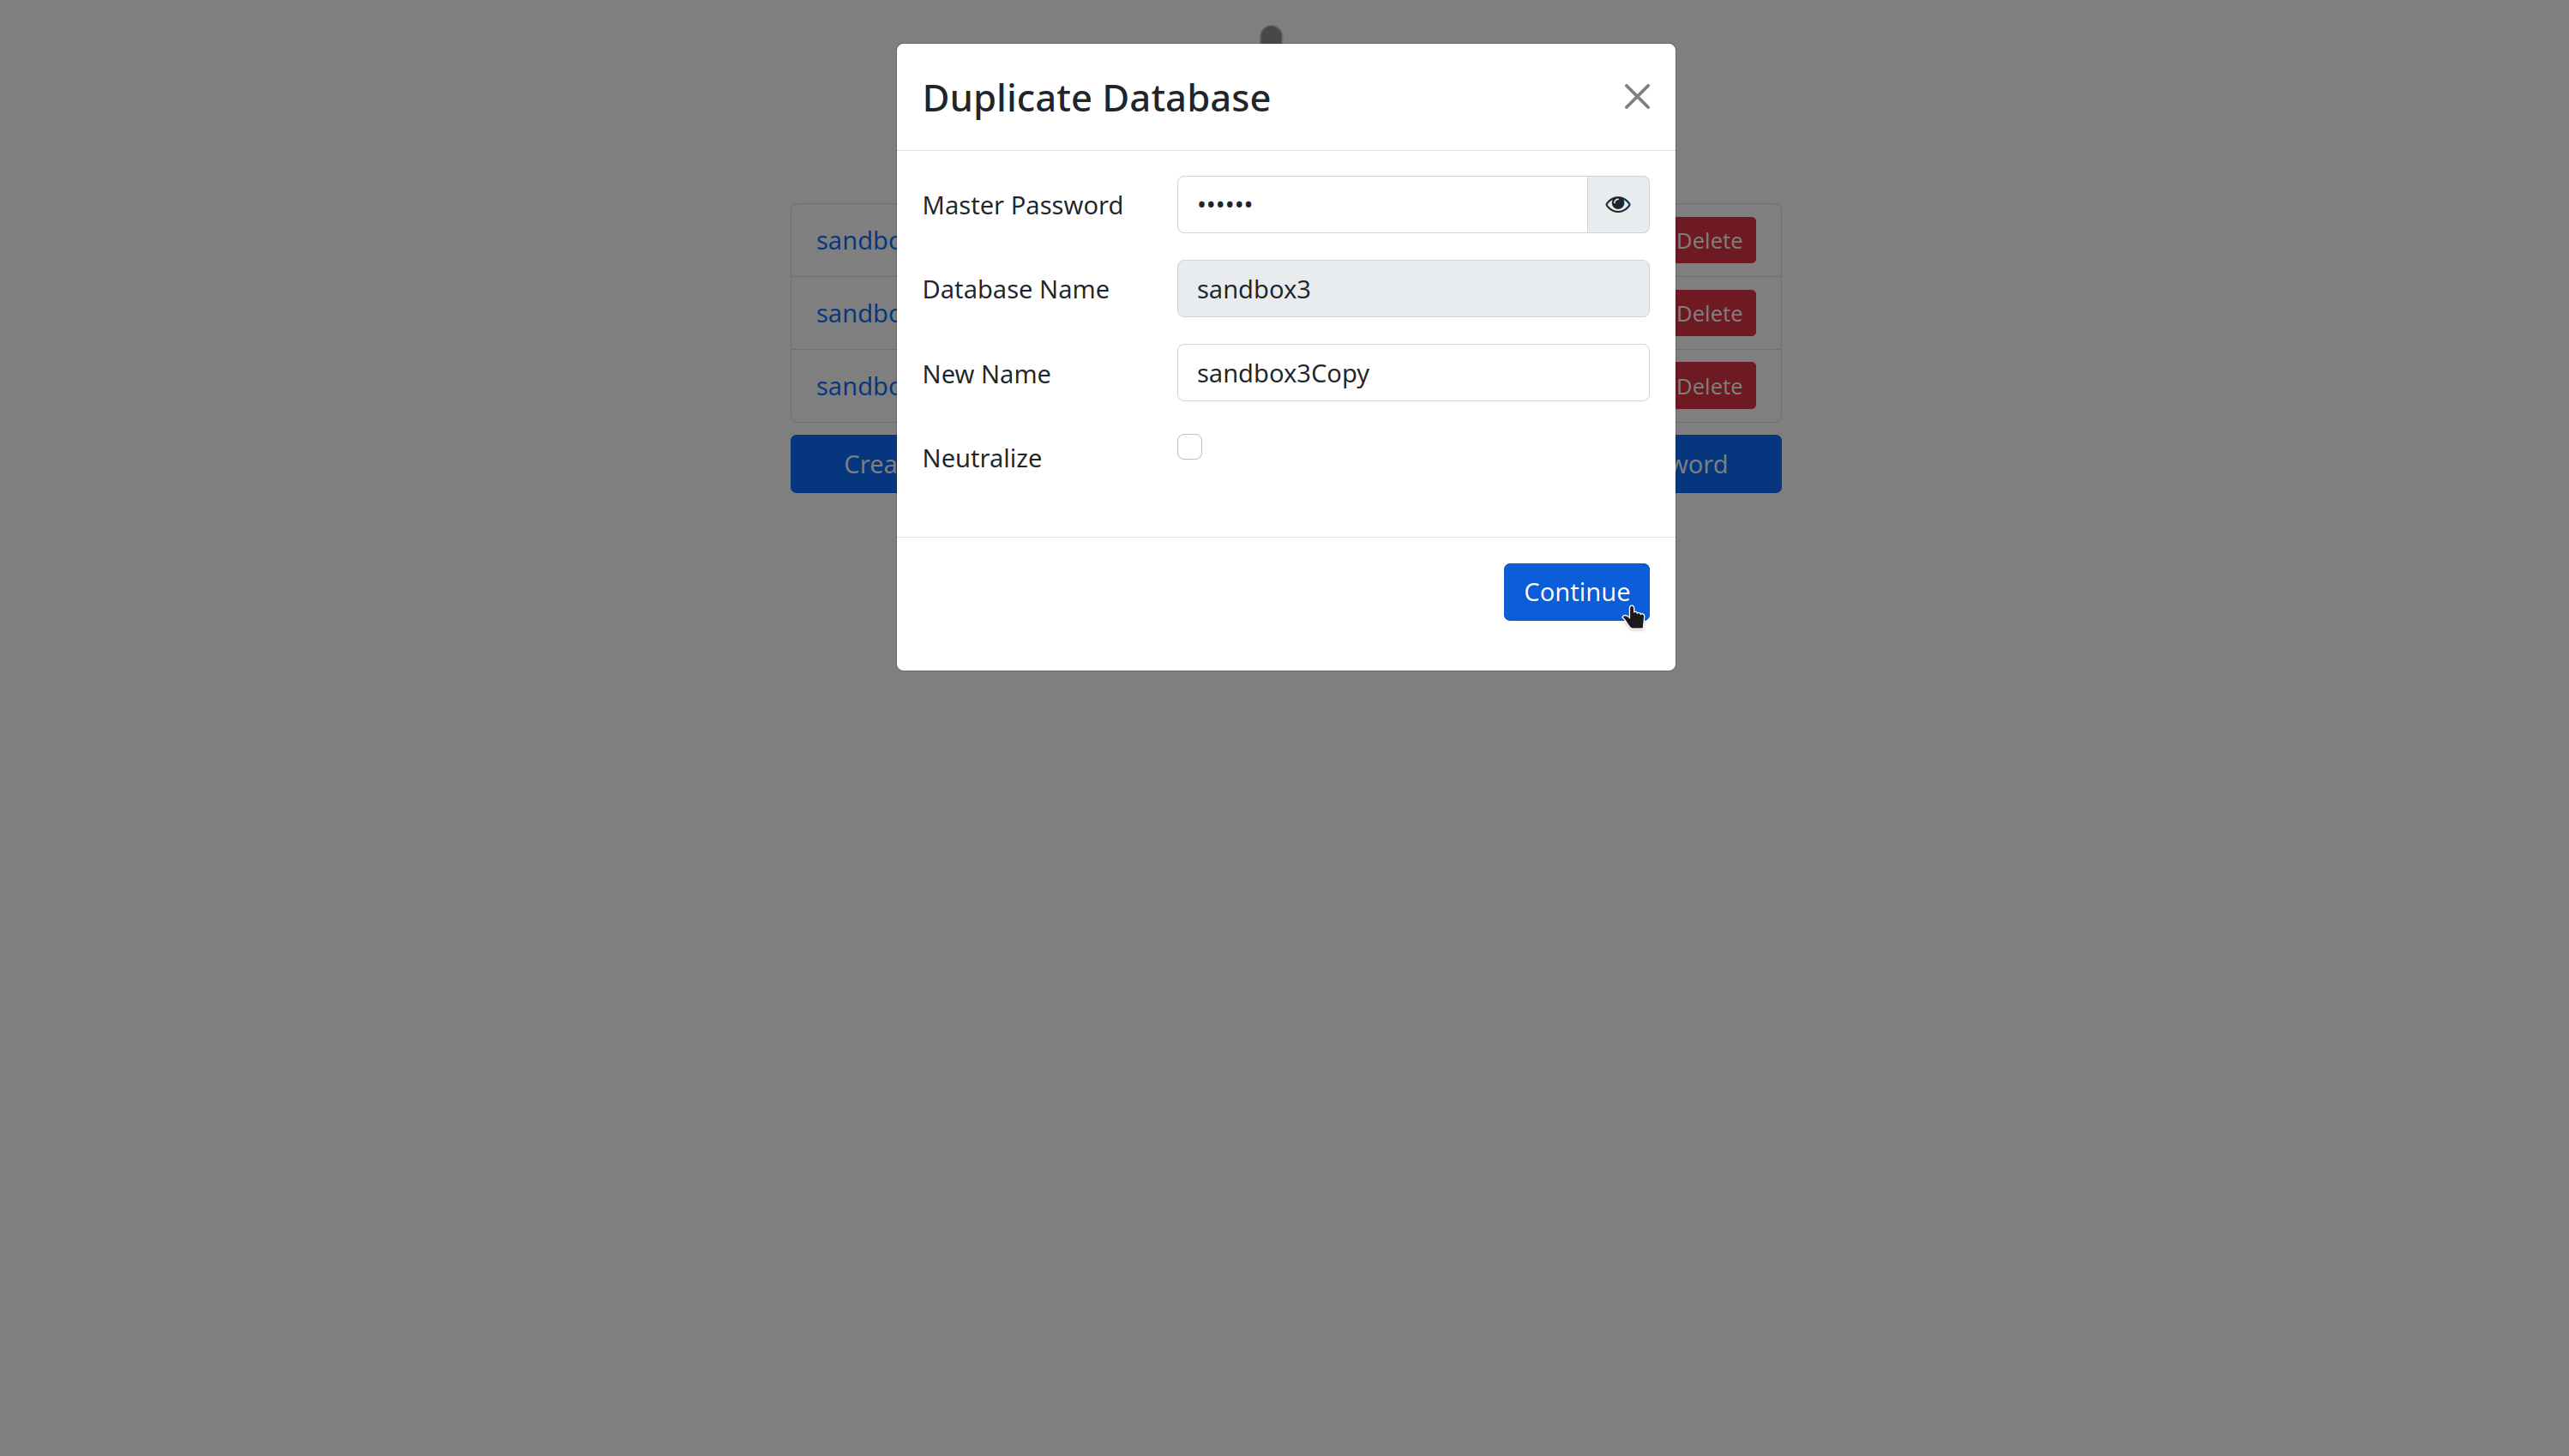
\includegraphics[width=6cm]{duplicarDb.png}
    \caption{Duplicación de una base de datos.}
    \label{fig:faqs}
\end{figure}
\paragraph{}
Al igual que en la creación de una base de datos, inicia sesión como si fuera la base de datos original.
\paragraph{}
Para eliminar una base de datos haz click en la opción de Delete de la base de datos a eliminar. Introduce la contraseña maestra y pulsa en Continue.
\begin{figure}[h]
    \centering
    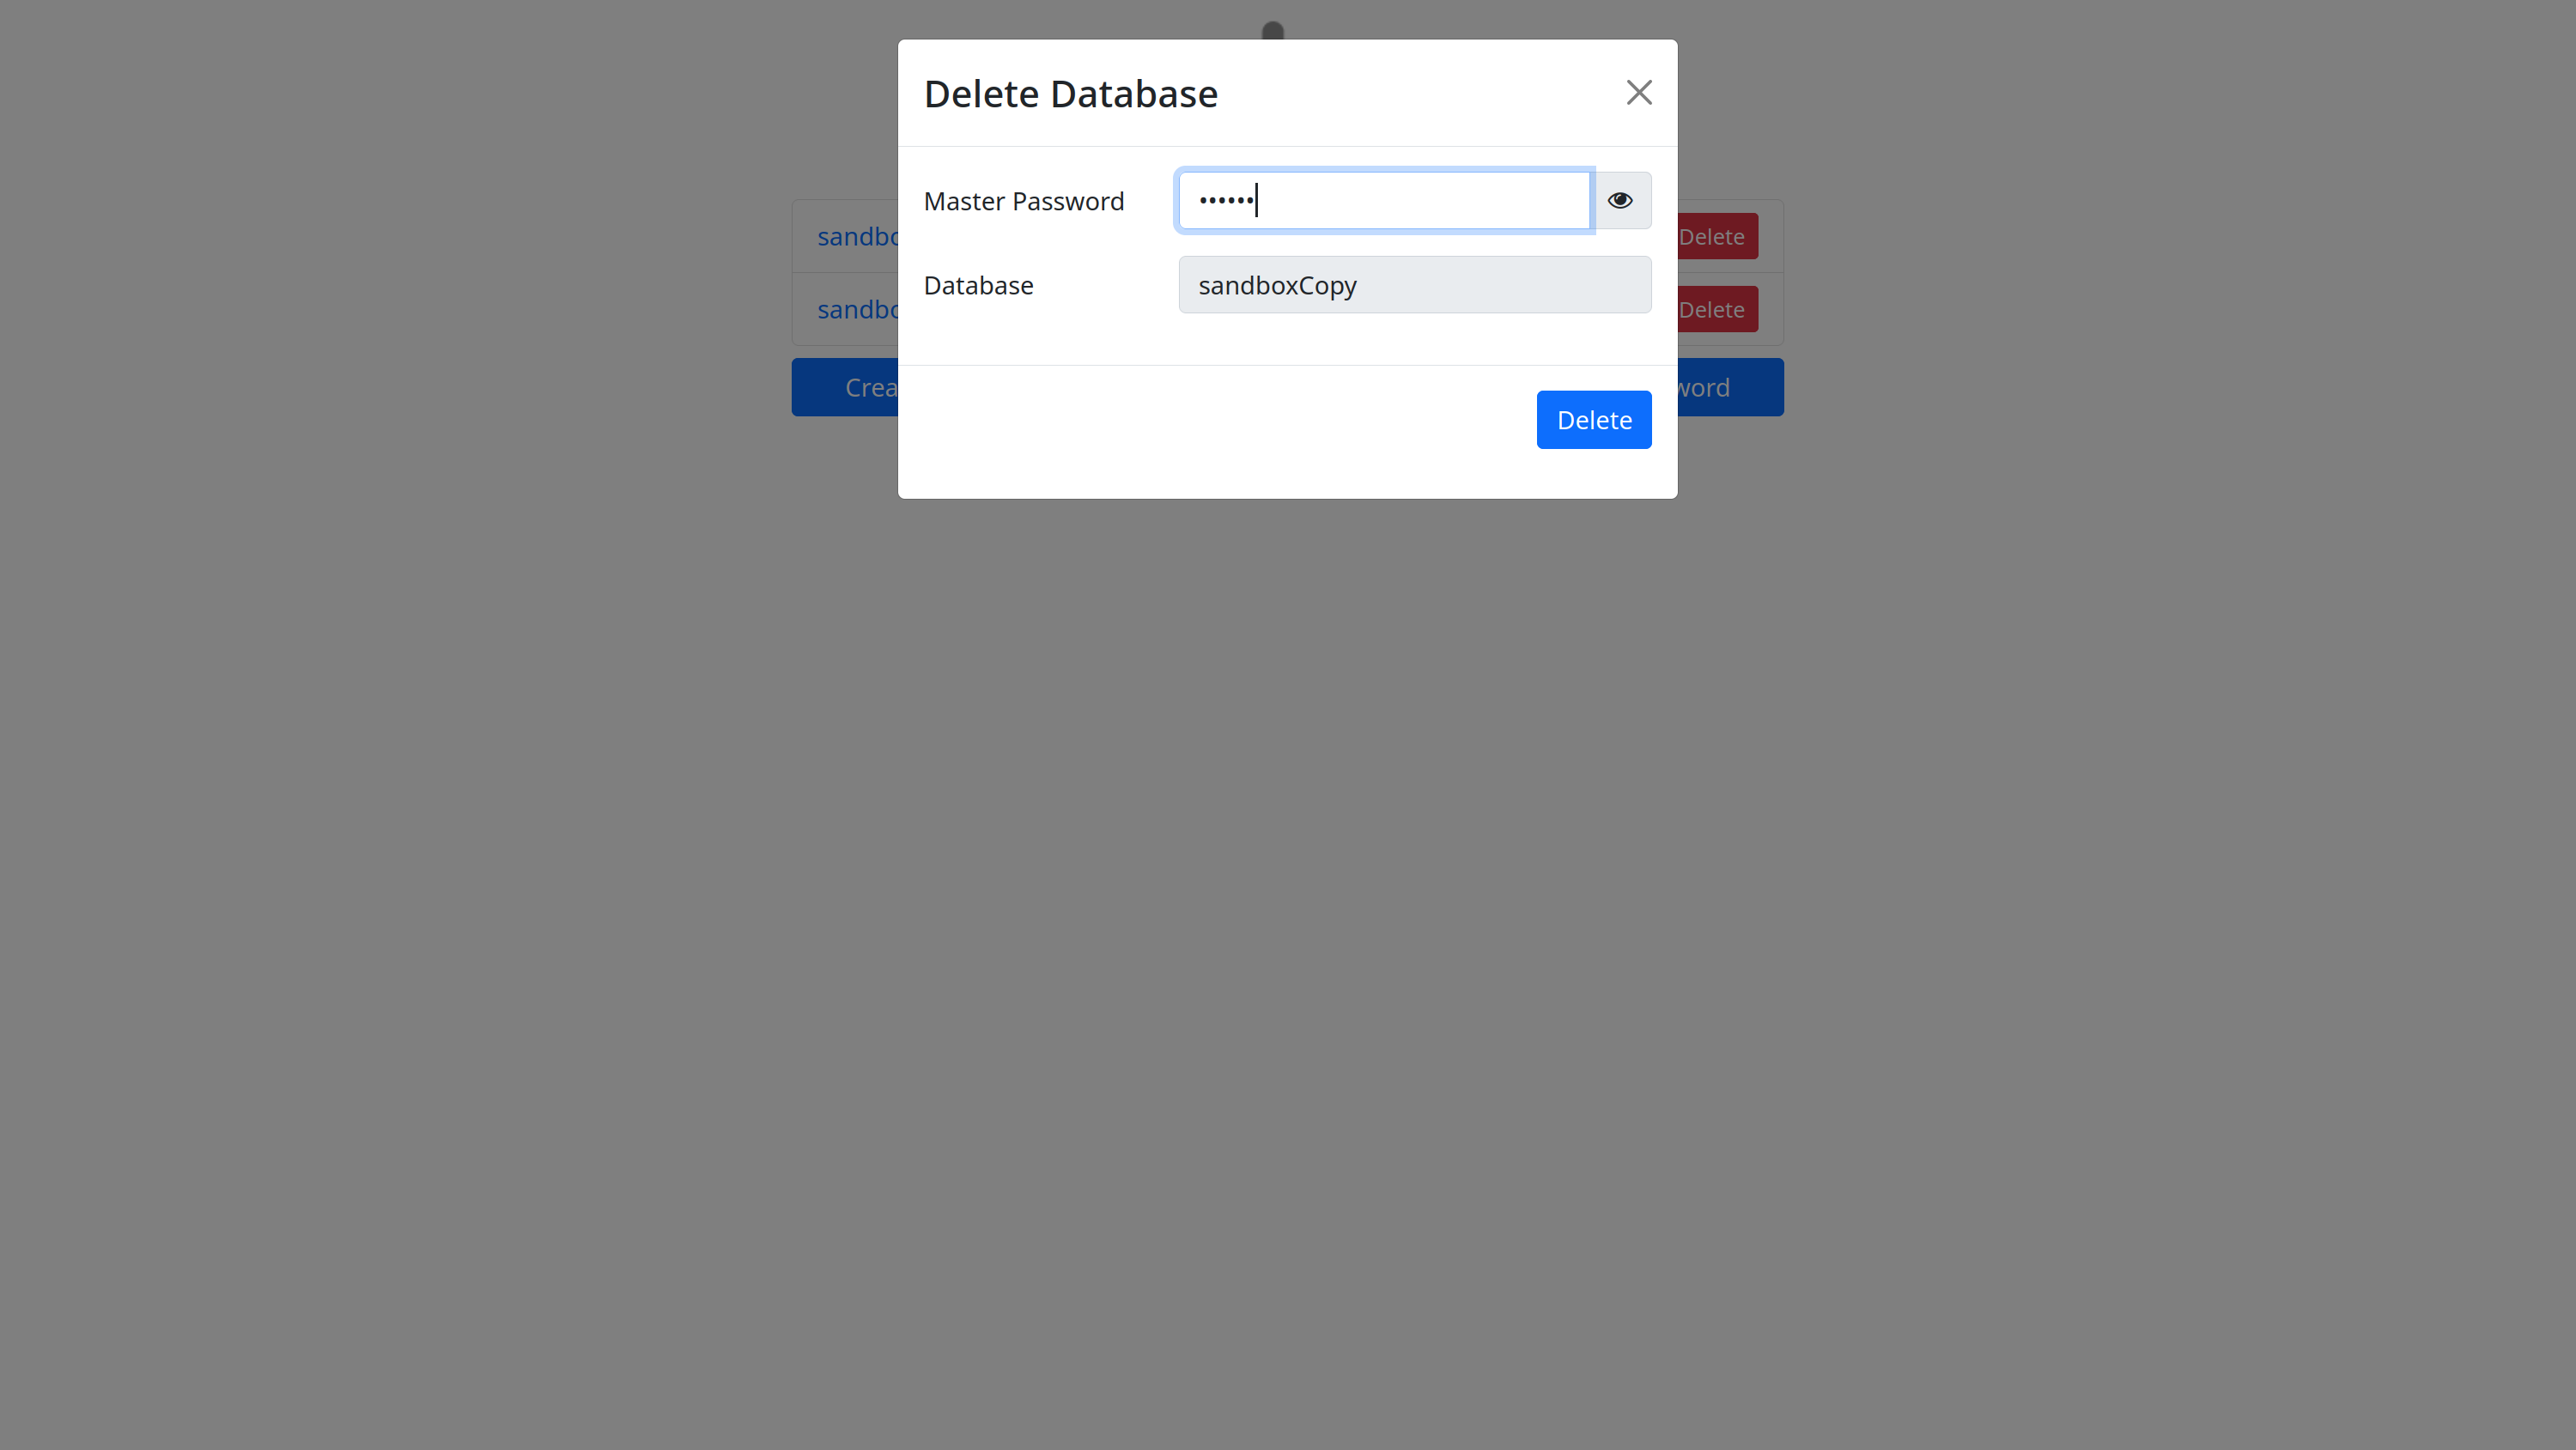
\includegraphics[width=6cm]{eliminarDb.png}
    \caption{Borrado de una base de datos.}
    \label{fig:faqs}
\end{figure}
\paragraph{}
Por último, Odoo ofrece la posibilidad de restaurar una base de datos. Pulsa en el botón Restore Database. Introduce la contraseña maestra, el nombre de la base de datos y selecciona la carpeta zip que contiene la base de datos a restaurar. Selecciona si es una base de datos copiada o movida si es por otra situación, pulsa en Continue y espera a que se restaure.
\newpage
\begin{figure}[h]
    \centering
    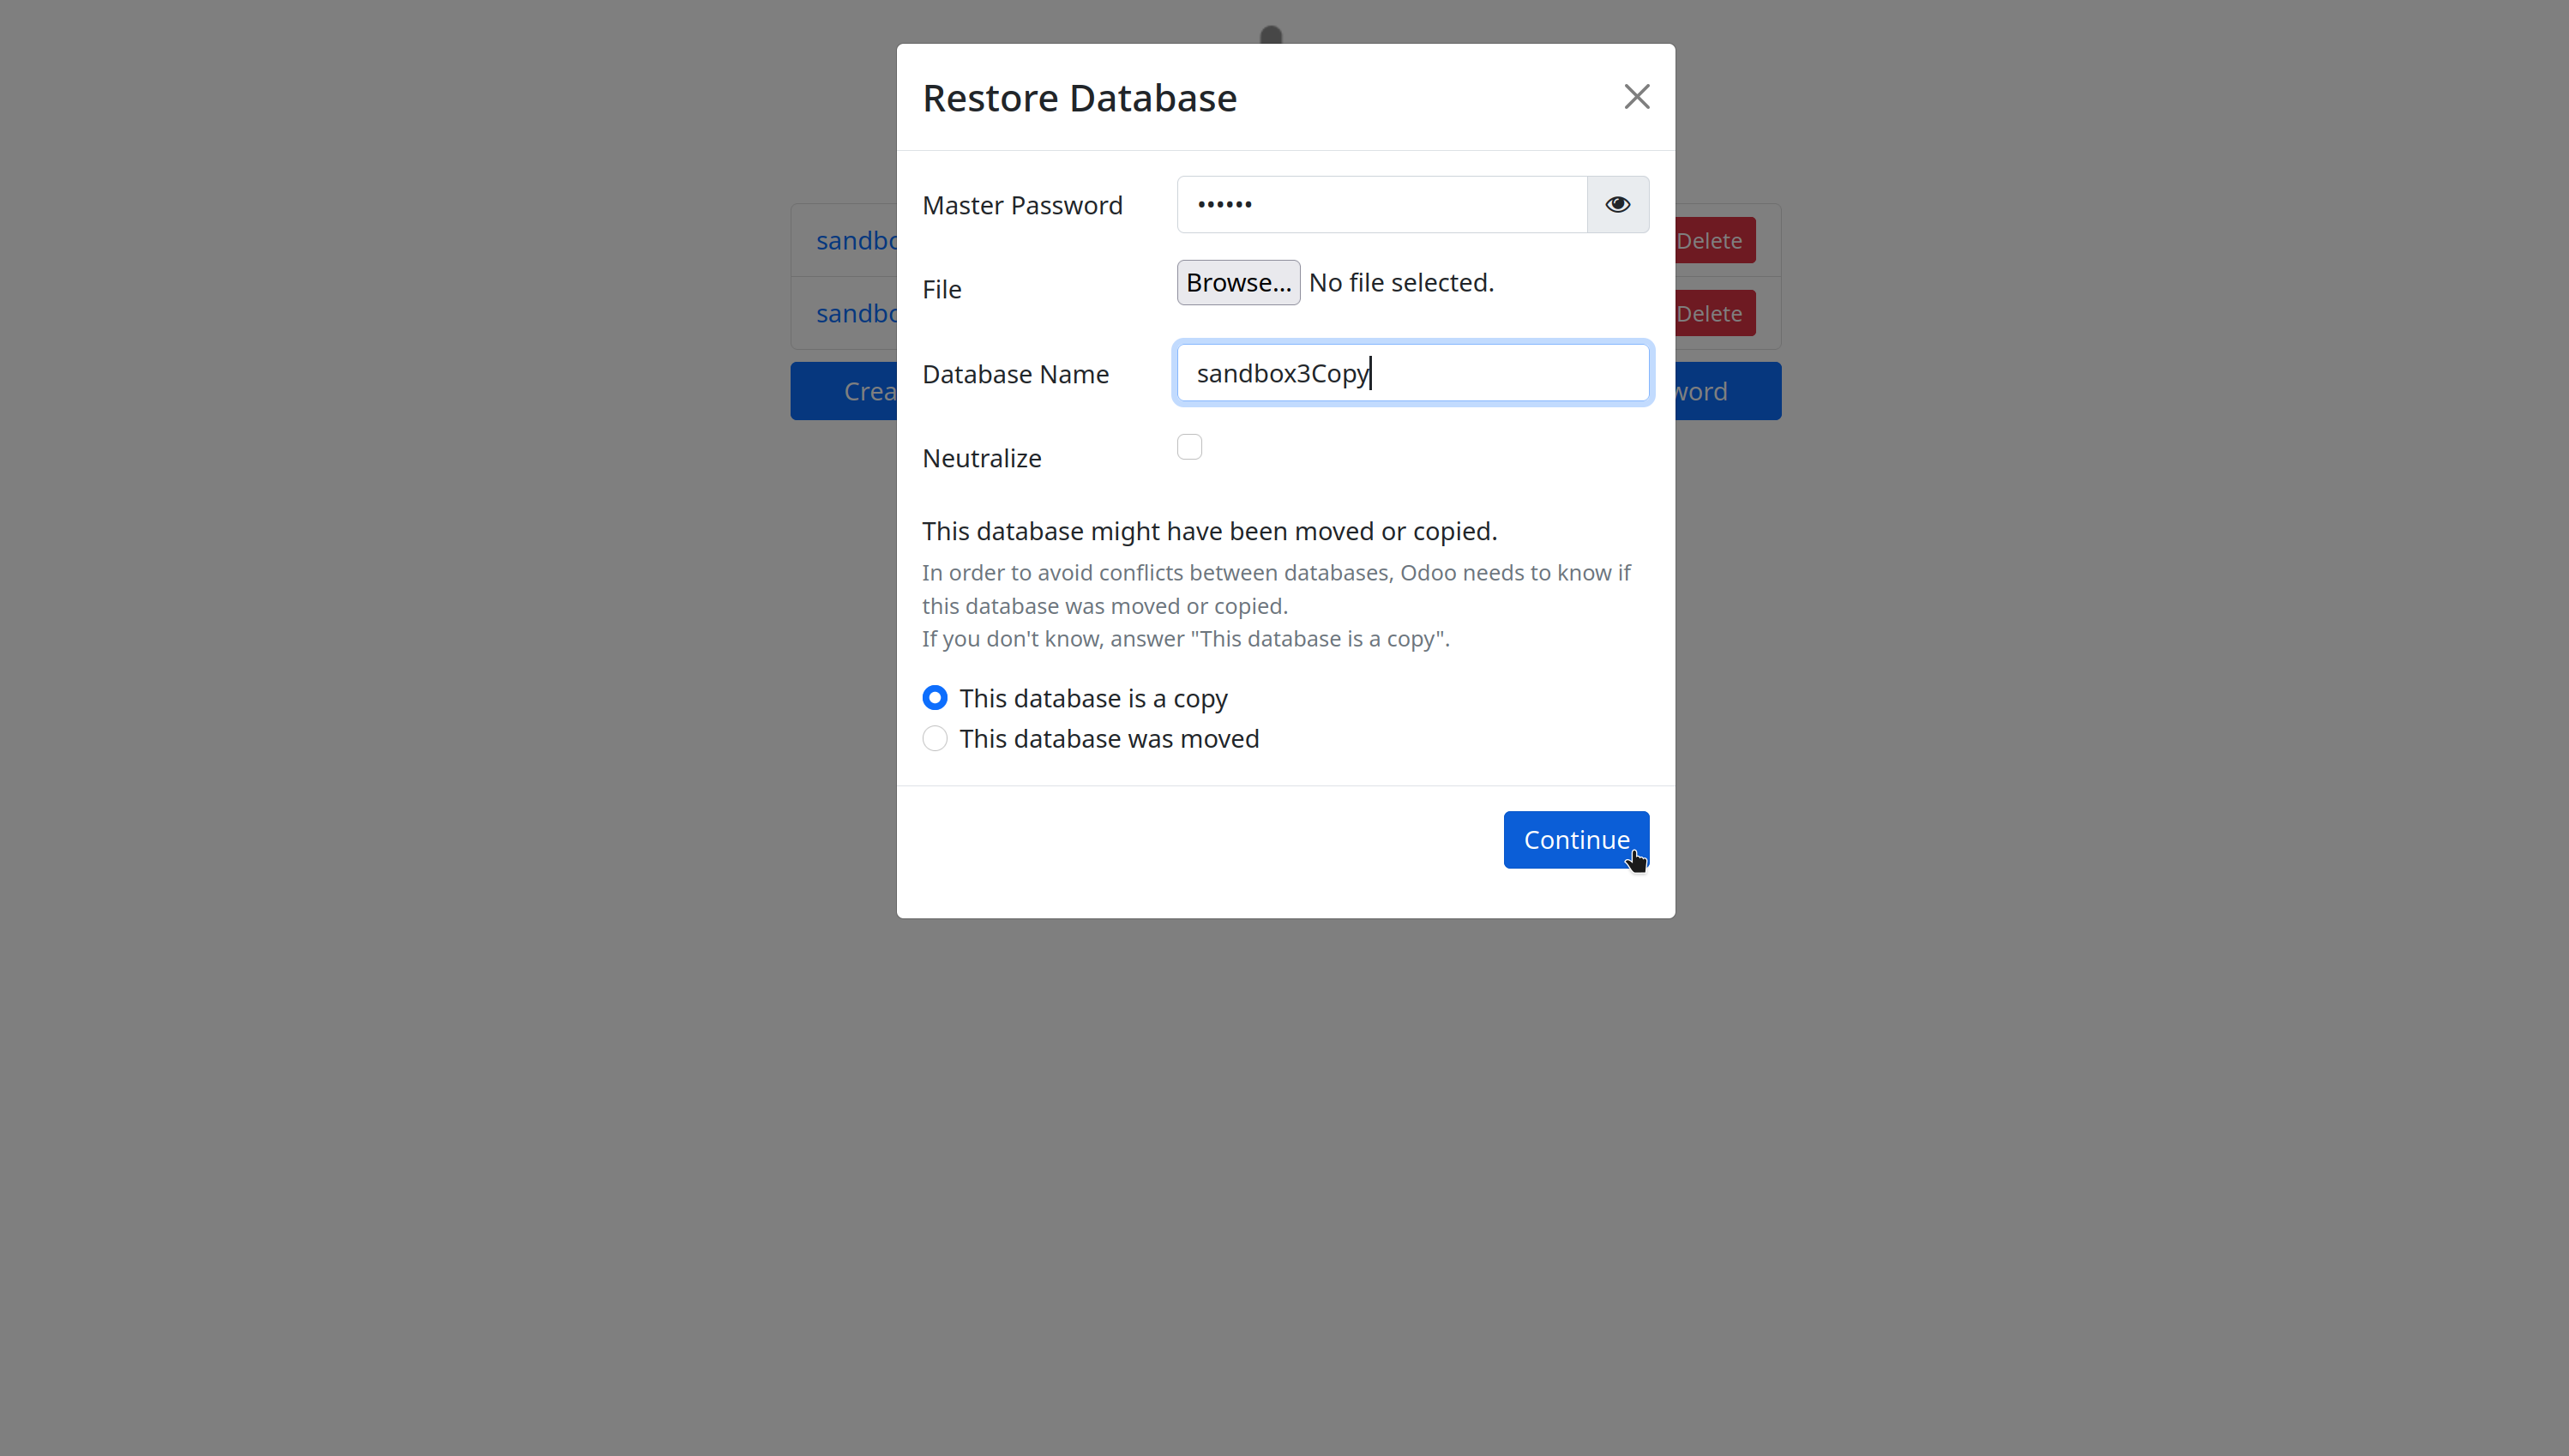
\includegraphics[width=6cm]{restaurarDb.png}
    \caption{Restauración de una base de datos.}
    \label{fig:faqs}
\end{figure}
\paragraph{}
Para llevar a cabo una transferencia de base de datos de una máquina a otra. Se debe realizar una copia de seguridad de la base de datos que se quiere transferir pulsando en la opción Backup dentro de la base de datos. 
\begin{figure}[h]
    \centering
    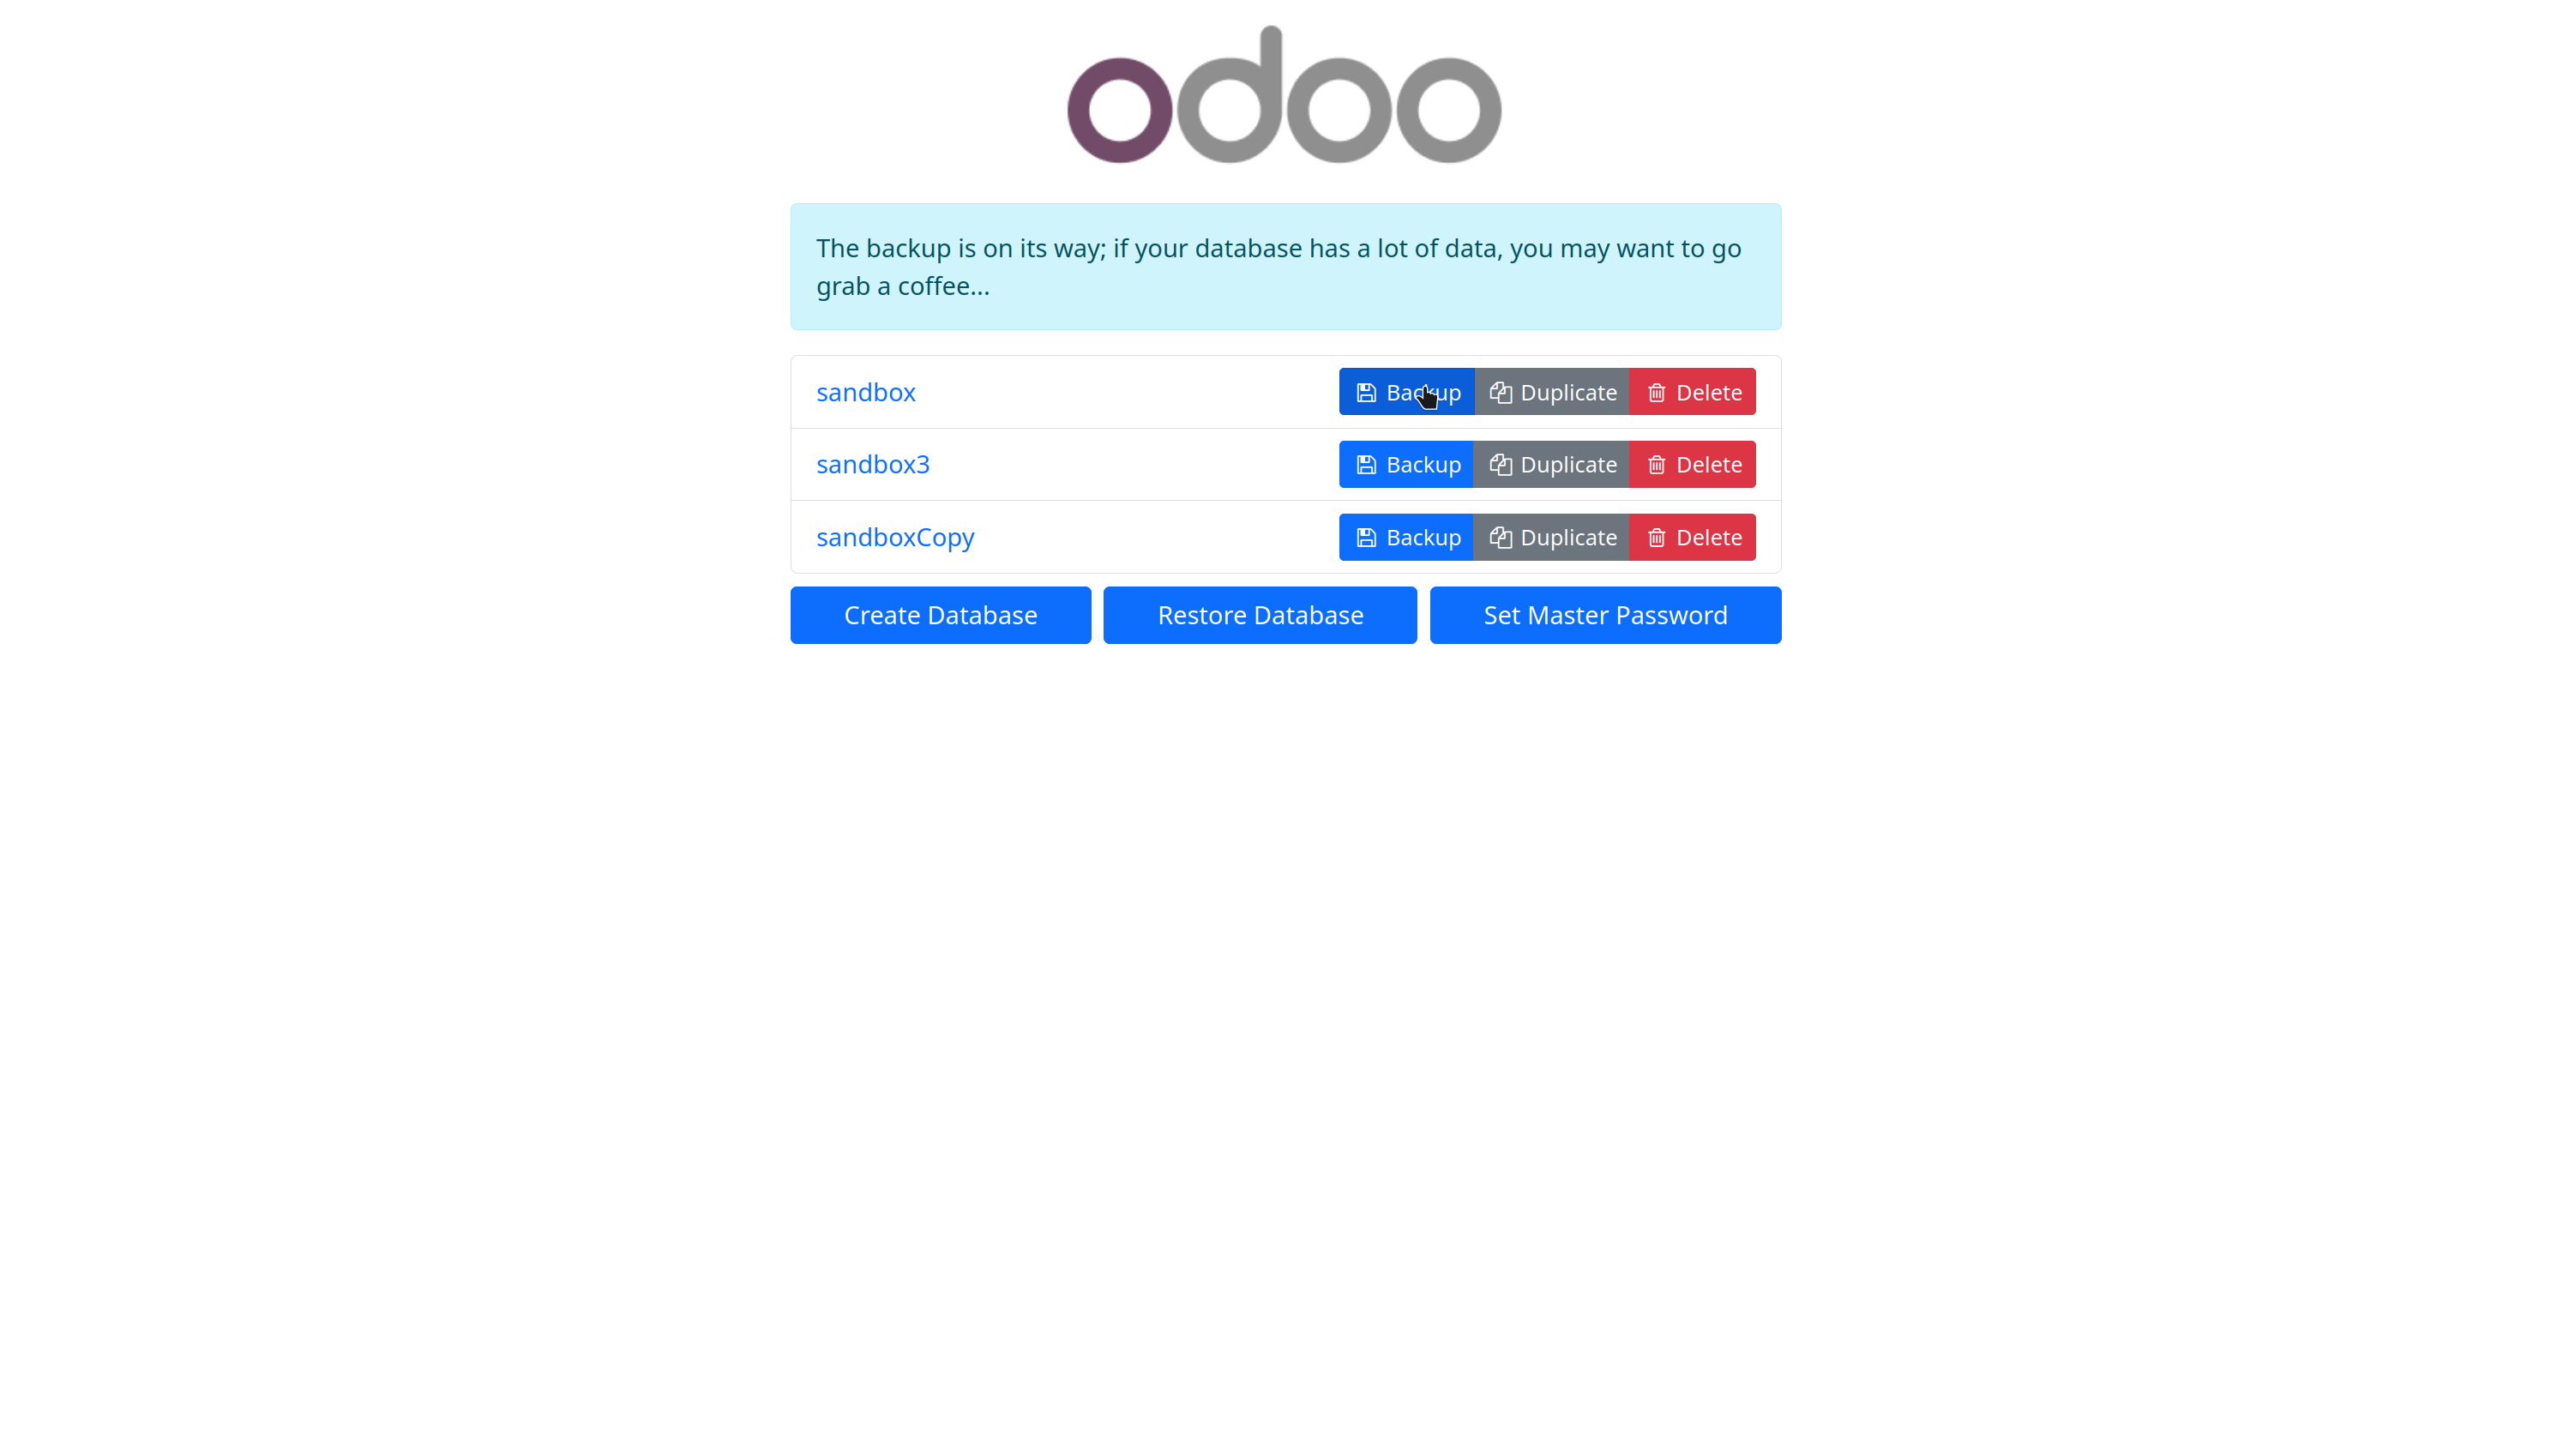
\includegraphics[width=6cm]{backupDb.png}
    \caption{Copia de seguridad de una base de datos.}
    \label{fig:faqs}
\end{figure}
\paragraph{}
A continuación, introduce la clave maestra, asegurate de que el formato es zip y pulsa en Continue.
\begin{figure}[h]
    \centering
    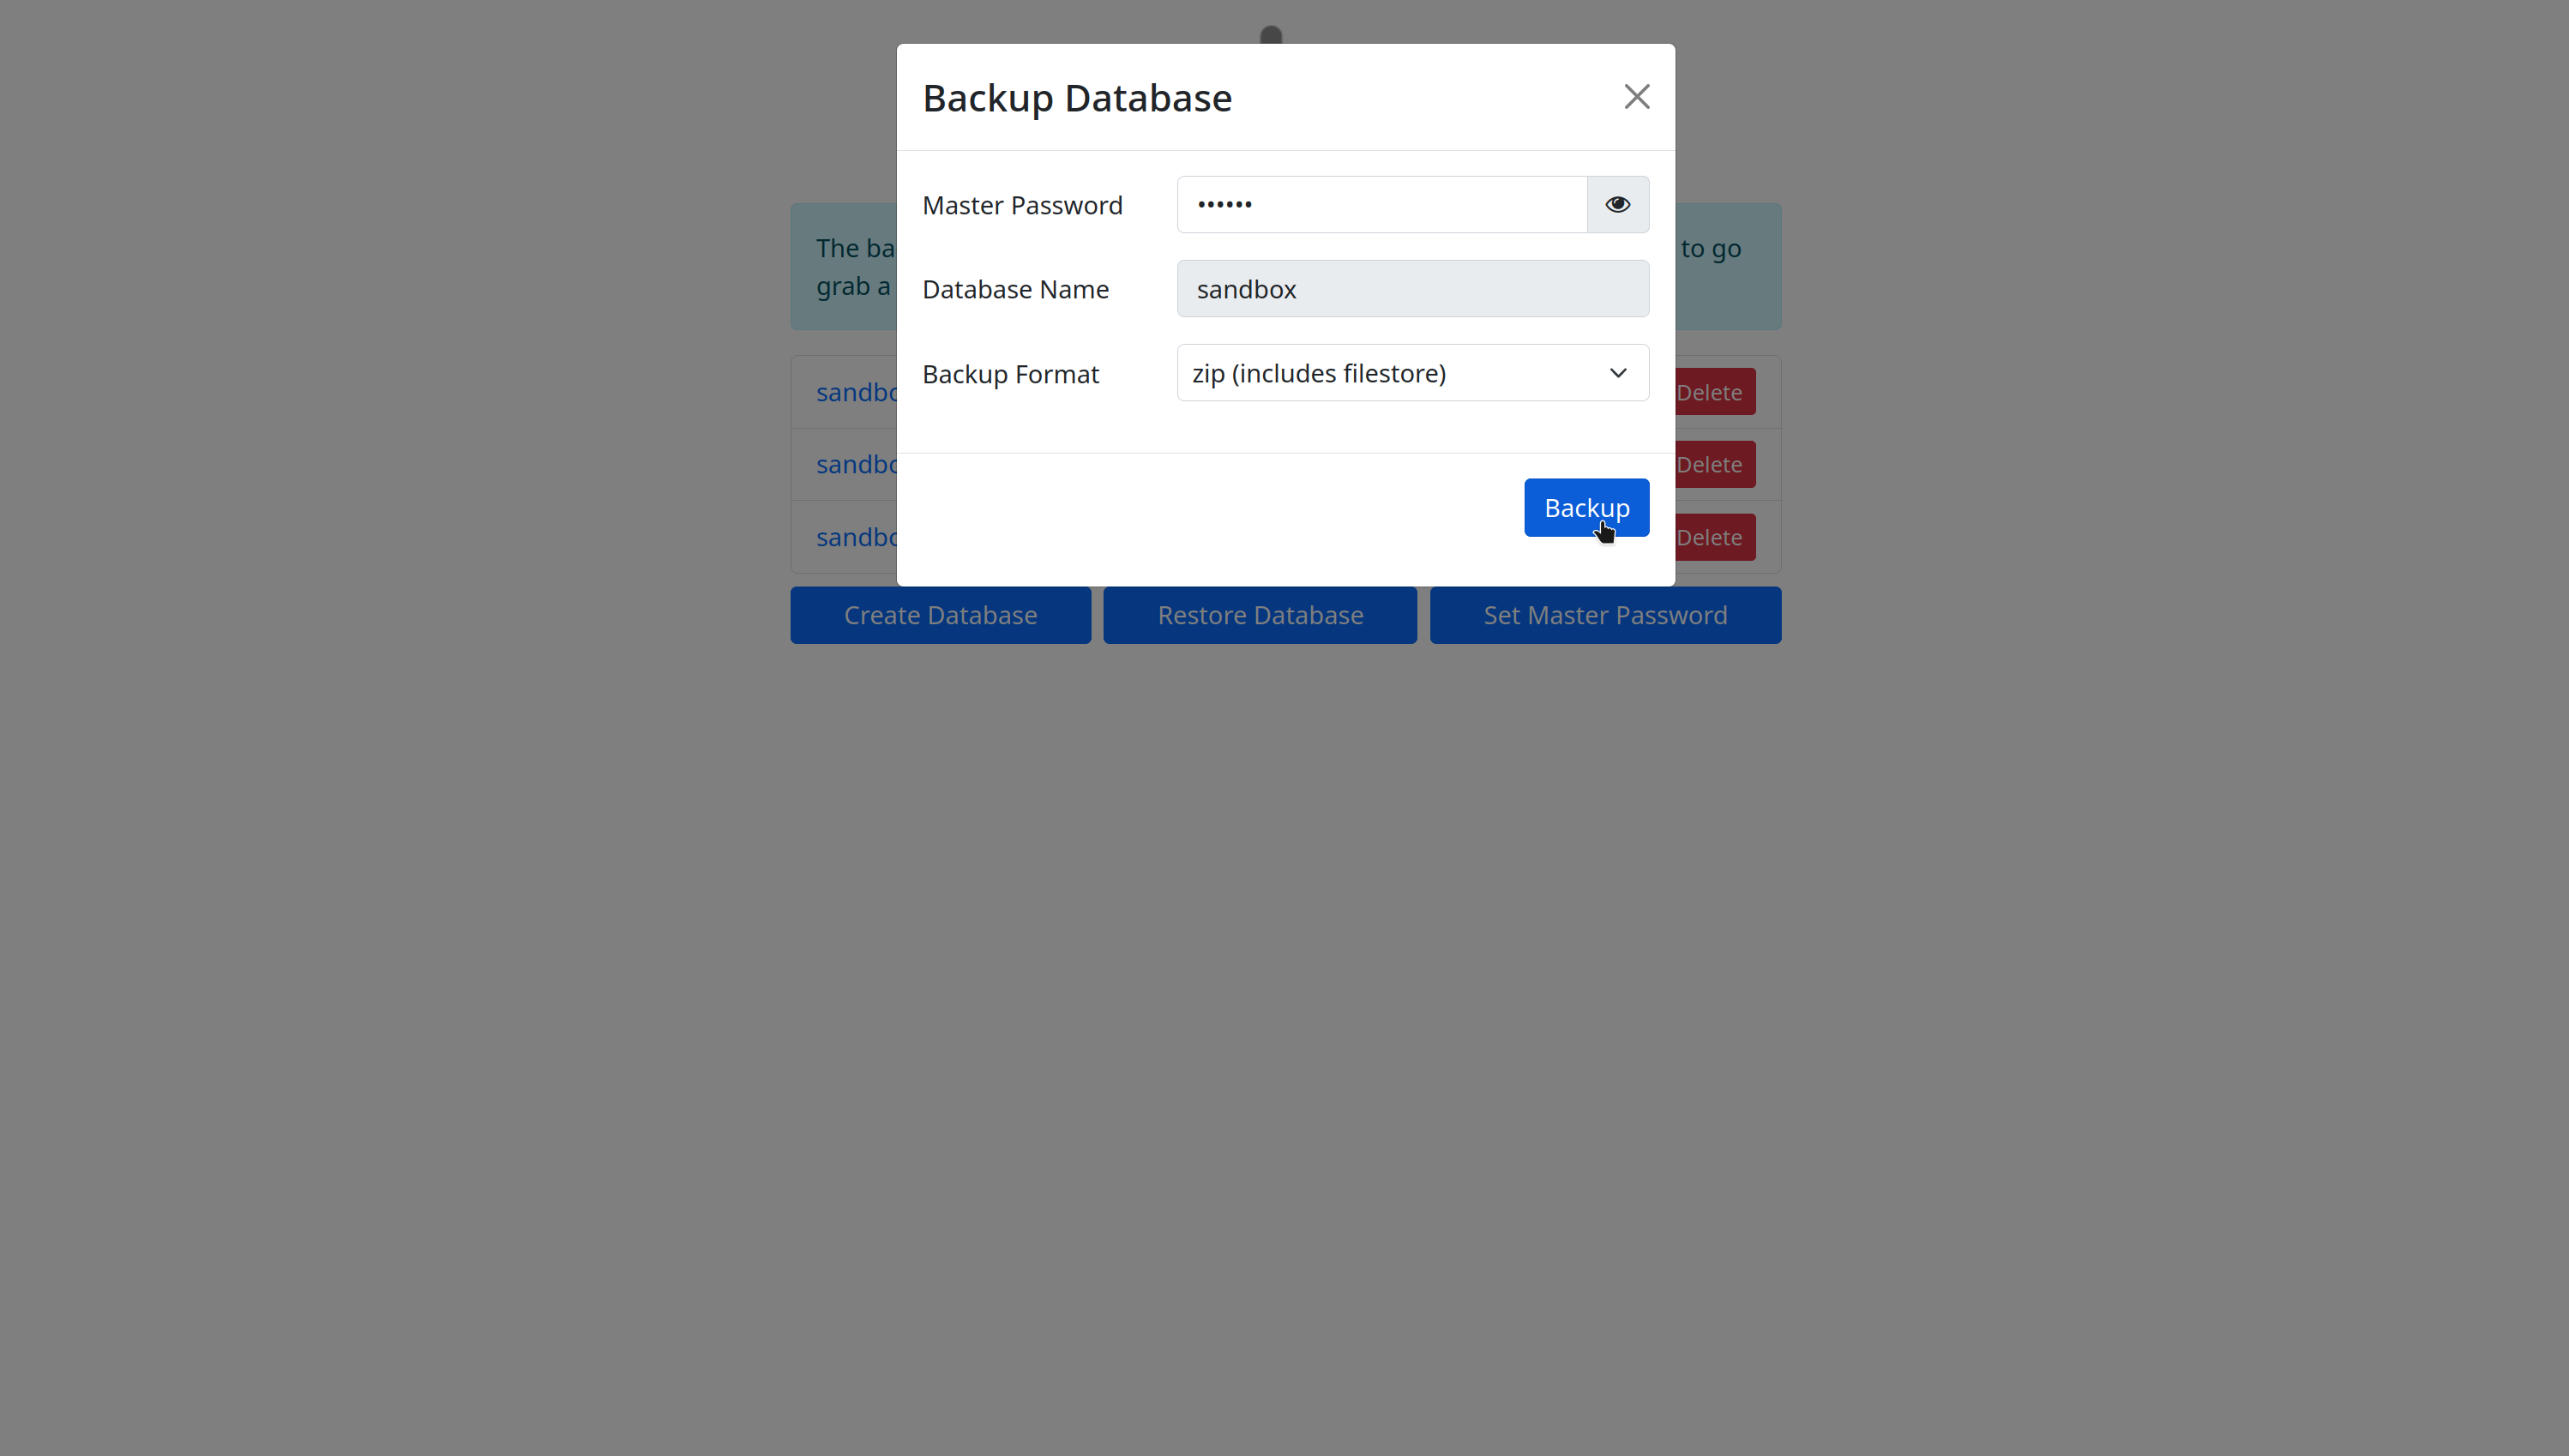
\includegraphics[width=6cm]{backupDb2.png}
    \caption{Copia de seguridad de una base de datos.}
    \label{fig:faqs}
\end{figure}
\paragraph{}
Cuando termine se habrá descargado en la máquina un zip con la base de datos. Por lo que ahora se podrá distribuir este zip a otra máquina y se podrá importar la base de datos. Para ello, se debe seguir los pasos que se han explicado anteriormente para restaurar una base de datos y seleccionando la carpeta zip que se ha descargado.
Al acceder a Odoo con esa base de datos se tendrá la misma información que se tenía en la máquina anterior.
\newpage
\section{Proyectos}
\paragraph{}
Odoo ofrece la posibilidad de administrar los proyectos de nuestra empresa. Para ello, debemos instalar el módulo "Proyectos" en la página de aplicaciones.
\begin{figure}[h]
    \centering
    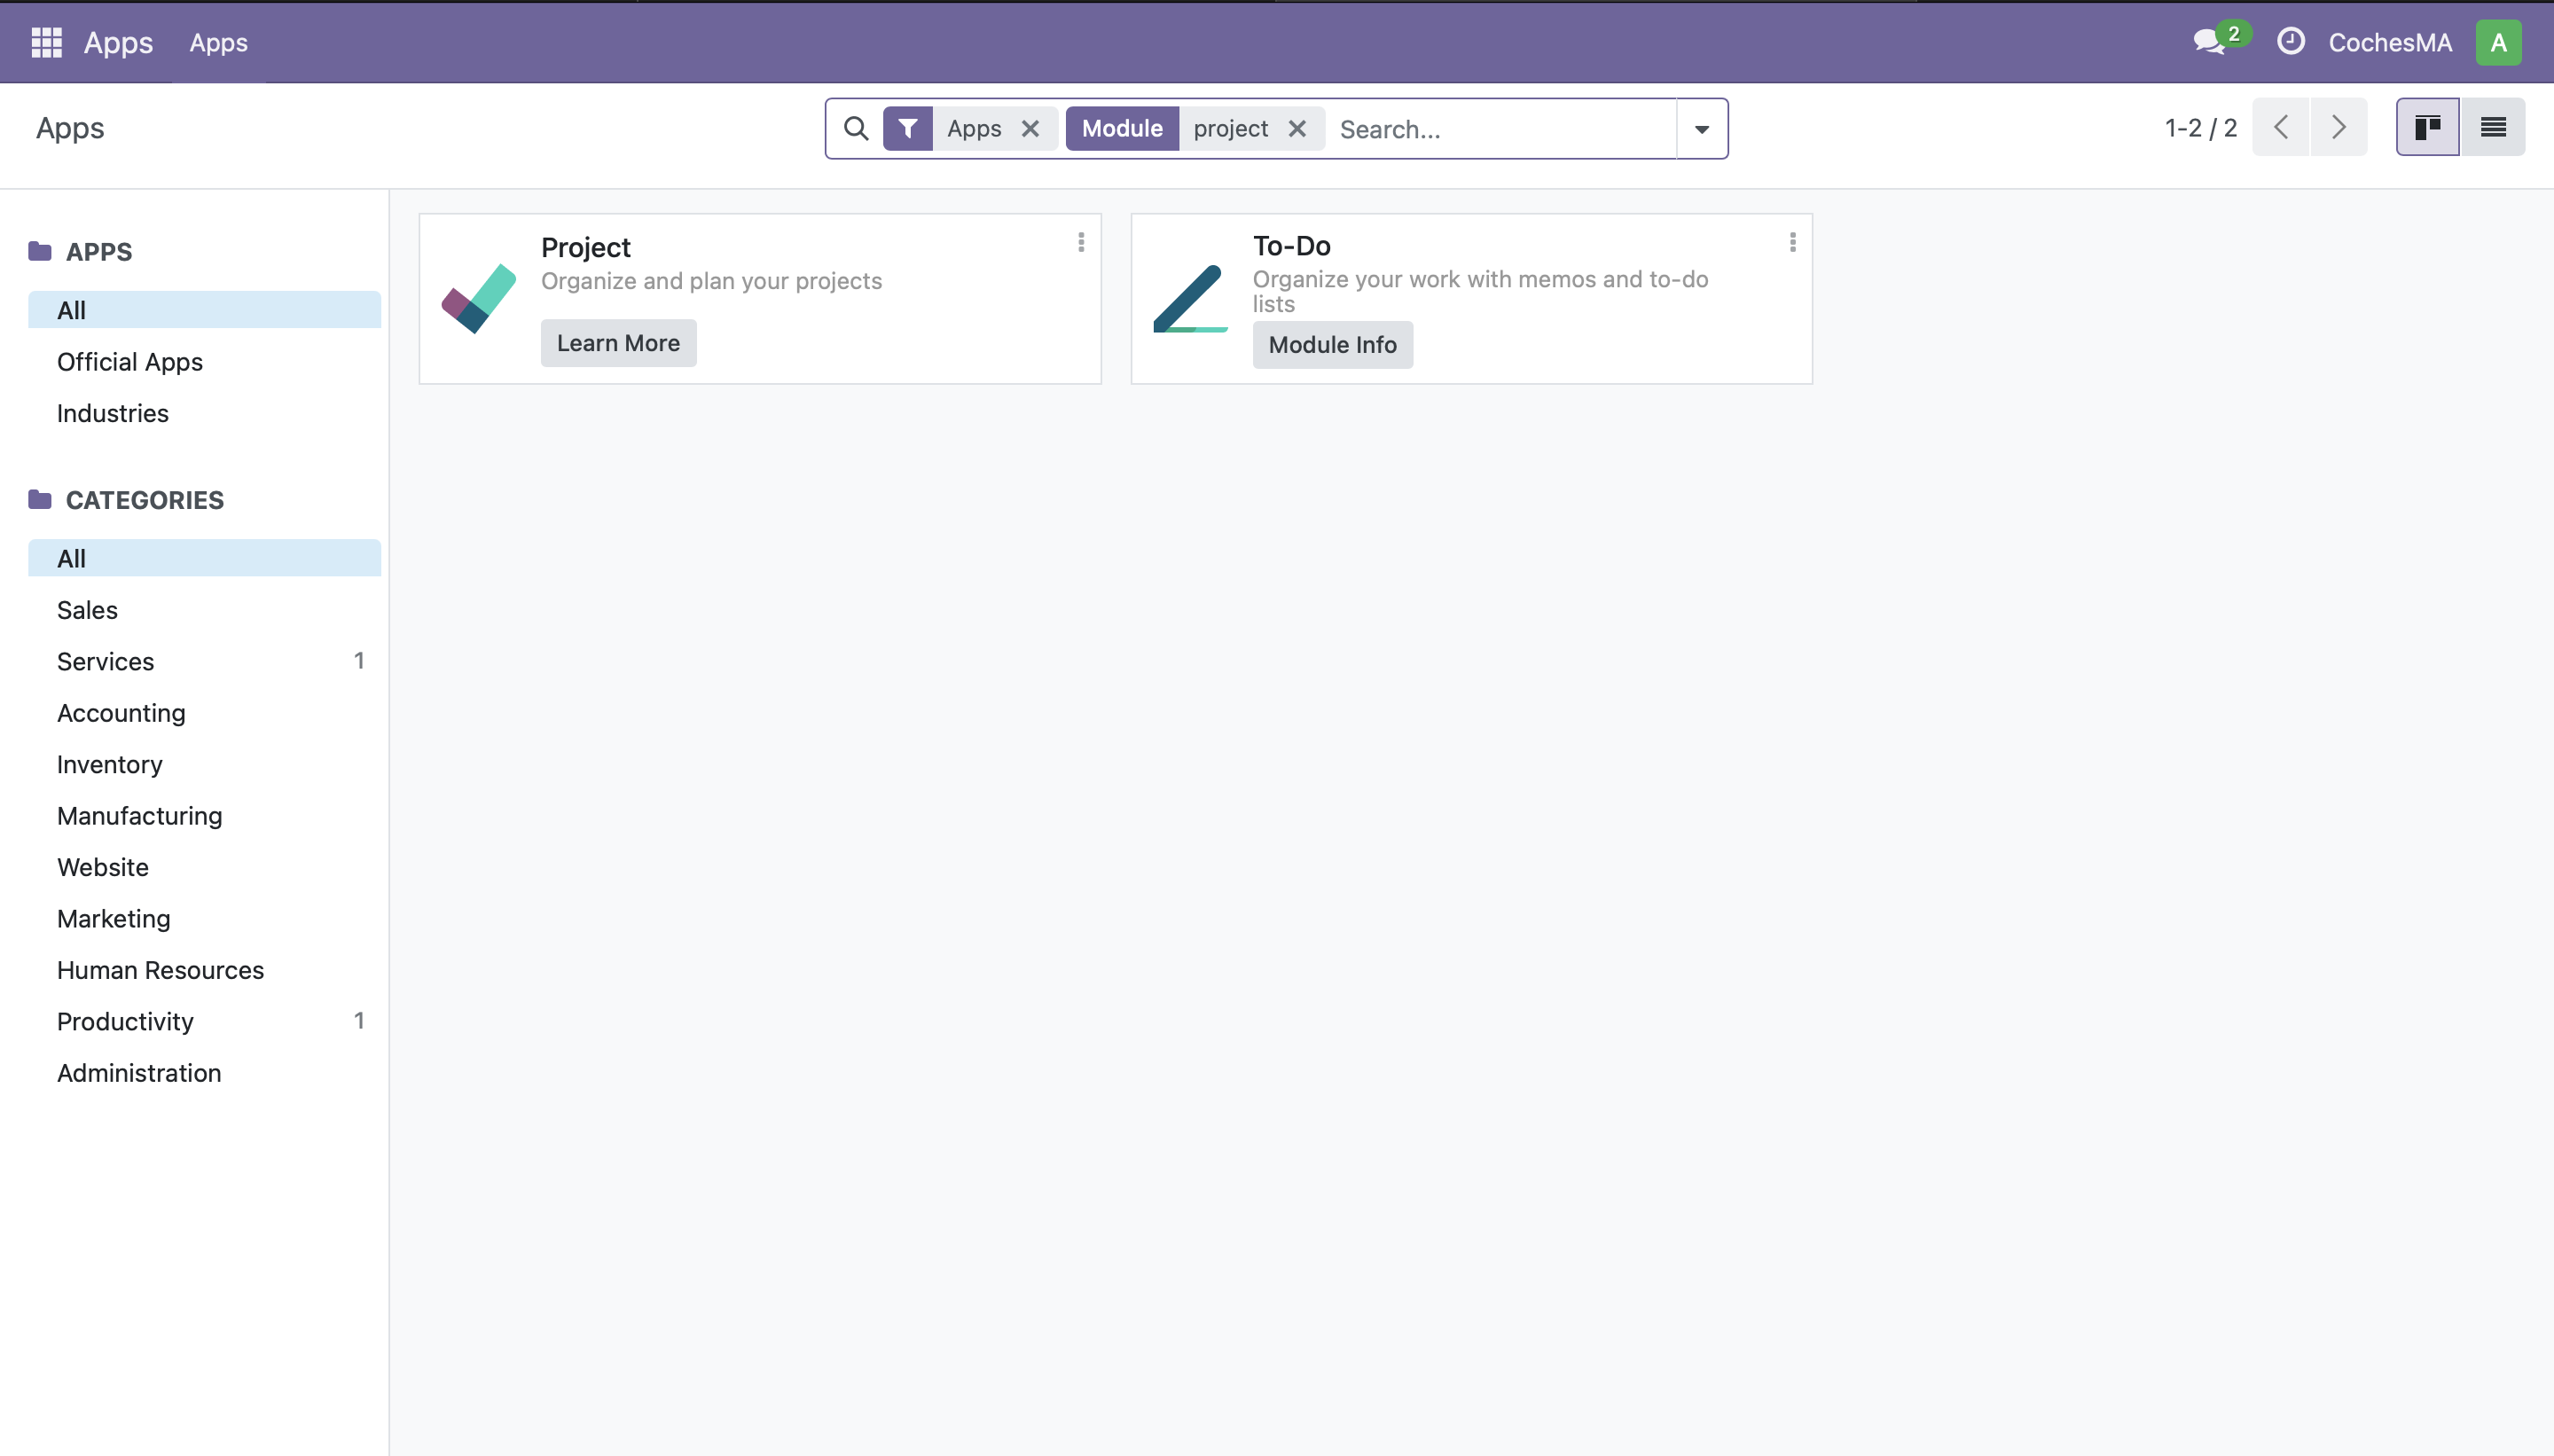
\includegraphics[width=10cm]{searchProject.png}
    \caption{Instalación del módulo de proyectos.}
    \label{fig:installProyectos}
\end{figure}
\paragraph{}
Una vez que hemos instalado podemos abrirlo pulsando en la esquina superior izquierda en el menú de aplicaciones y seleccionando la opción de Proyectos.
\begin{figure}[h]
    \centering
    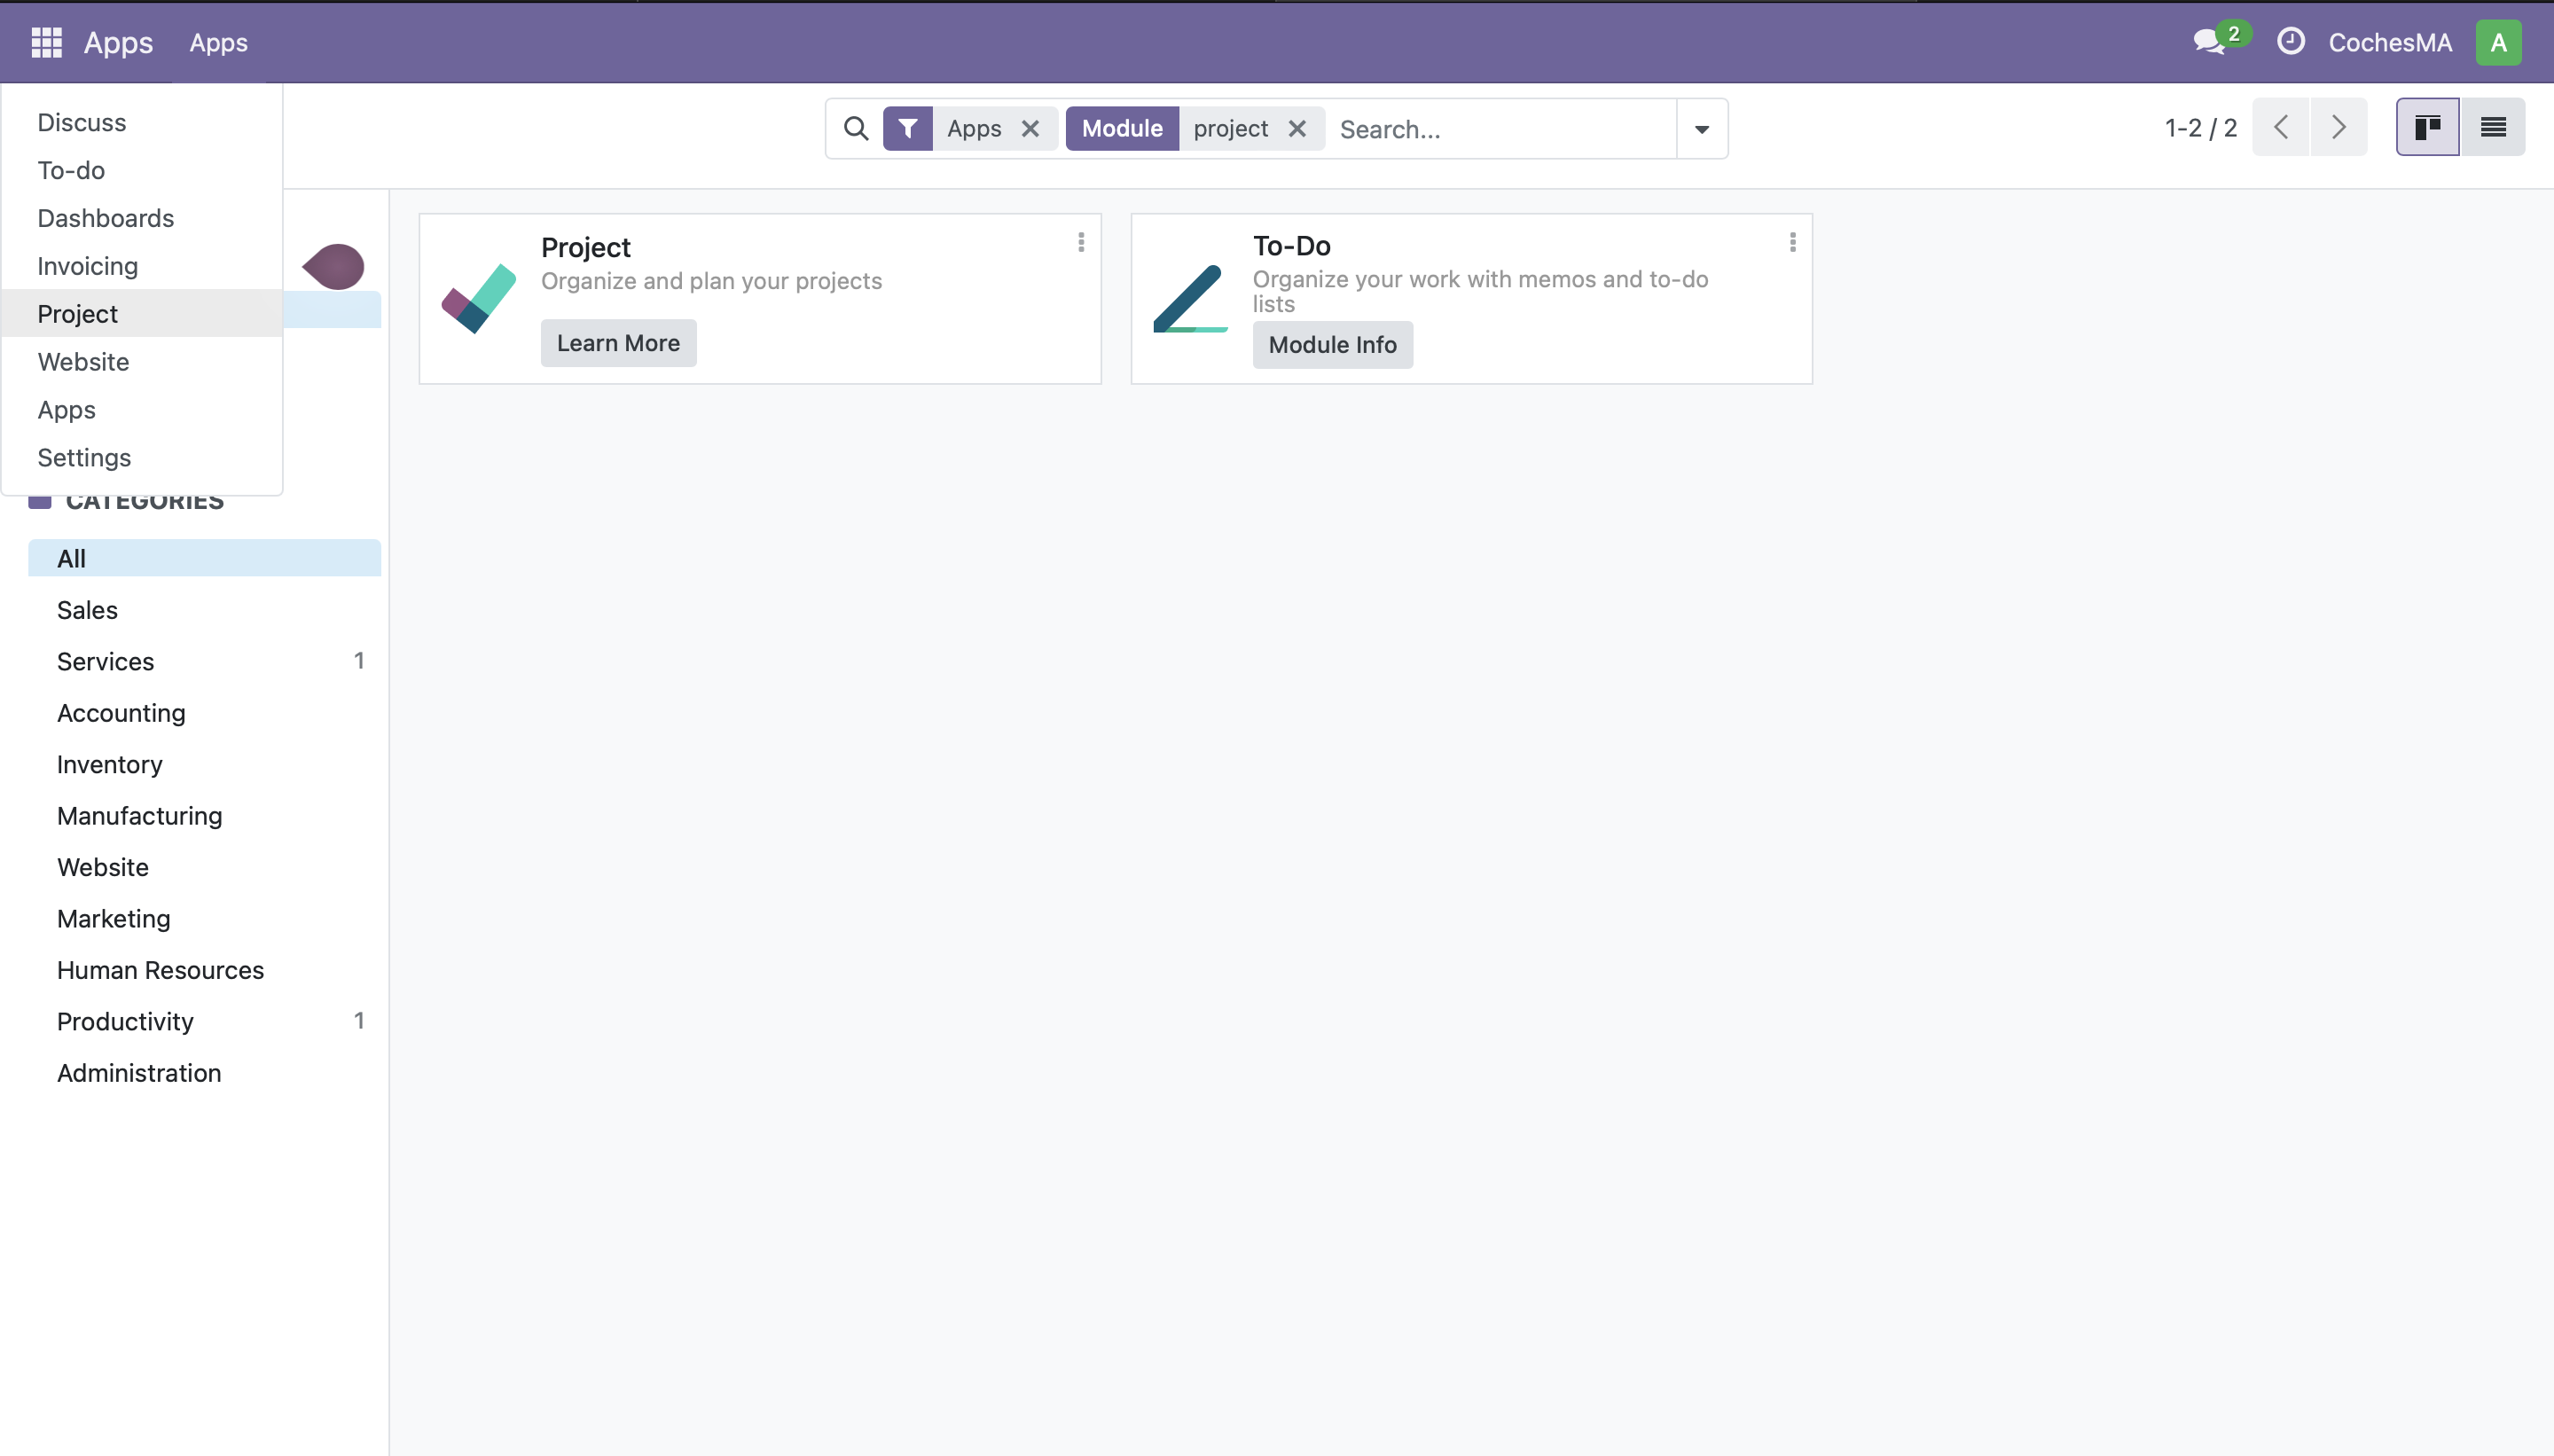
\includegraphics[width=10cm]{openProject.png}
    \caption{Abrir del módulo de proyectos.}
    \label{fig:openProyectos}
\end{figure}
\newpage
\paragraph{}
Al abrir el módulo de proyectos, se nos mostrará una lista de proyectos que se han creado. Al ser la primera vez que lo abrimos no existe ningun proyecto.

\begin{figure}[h]
    \centering
    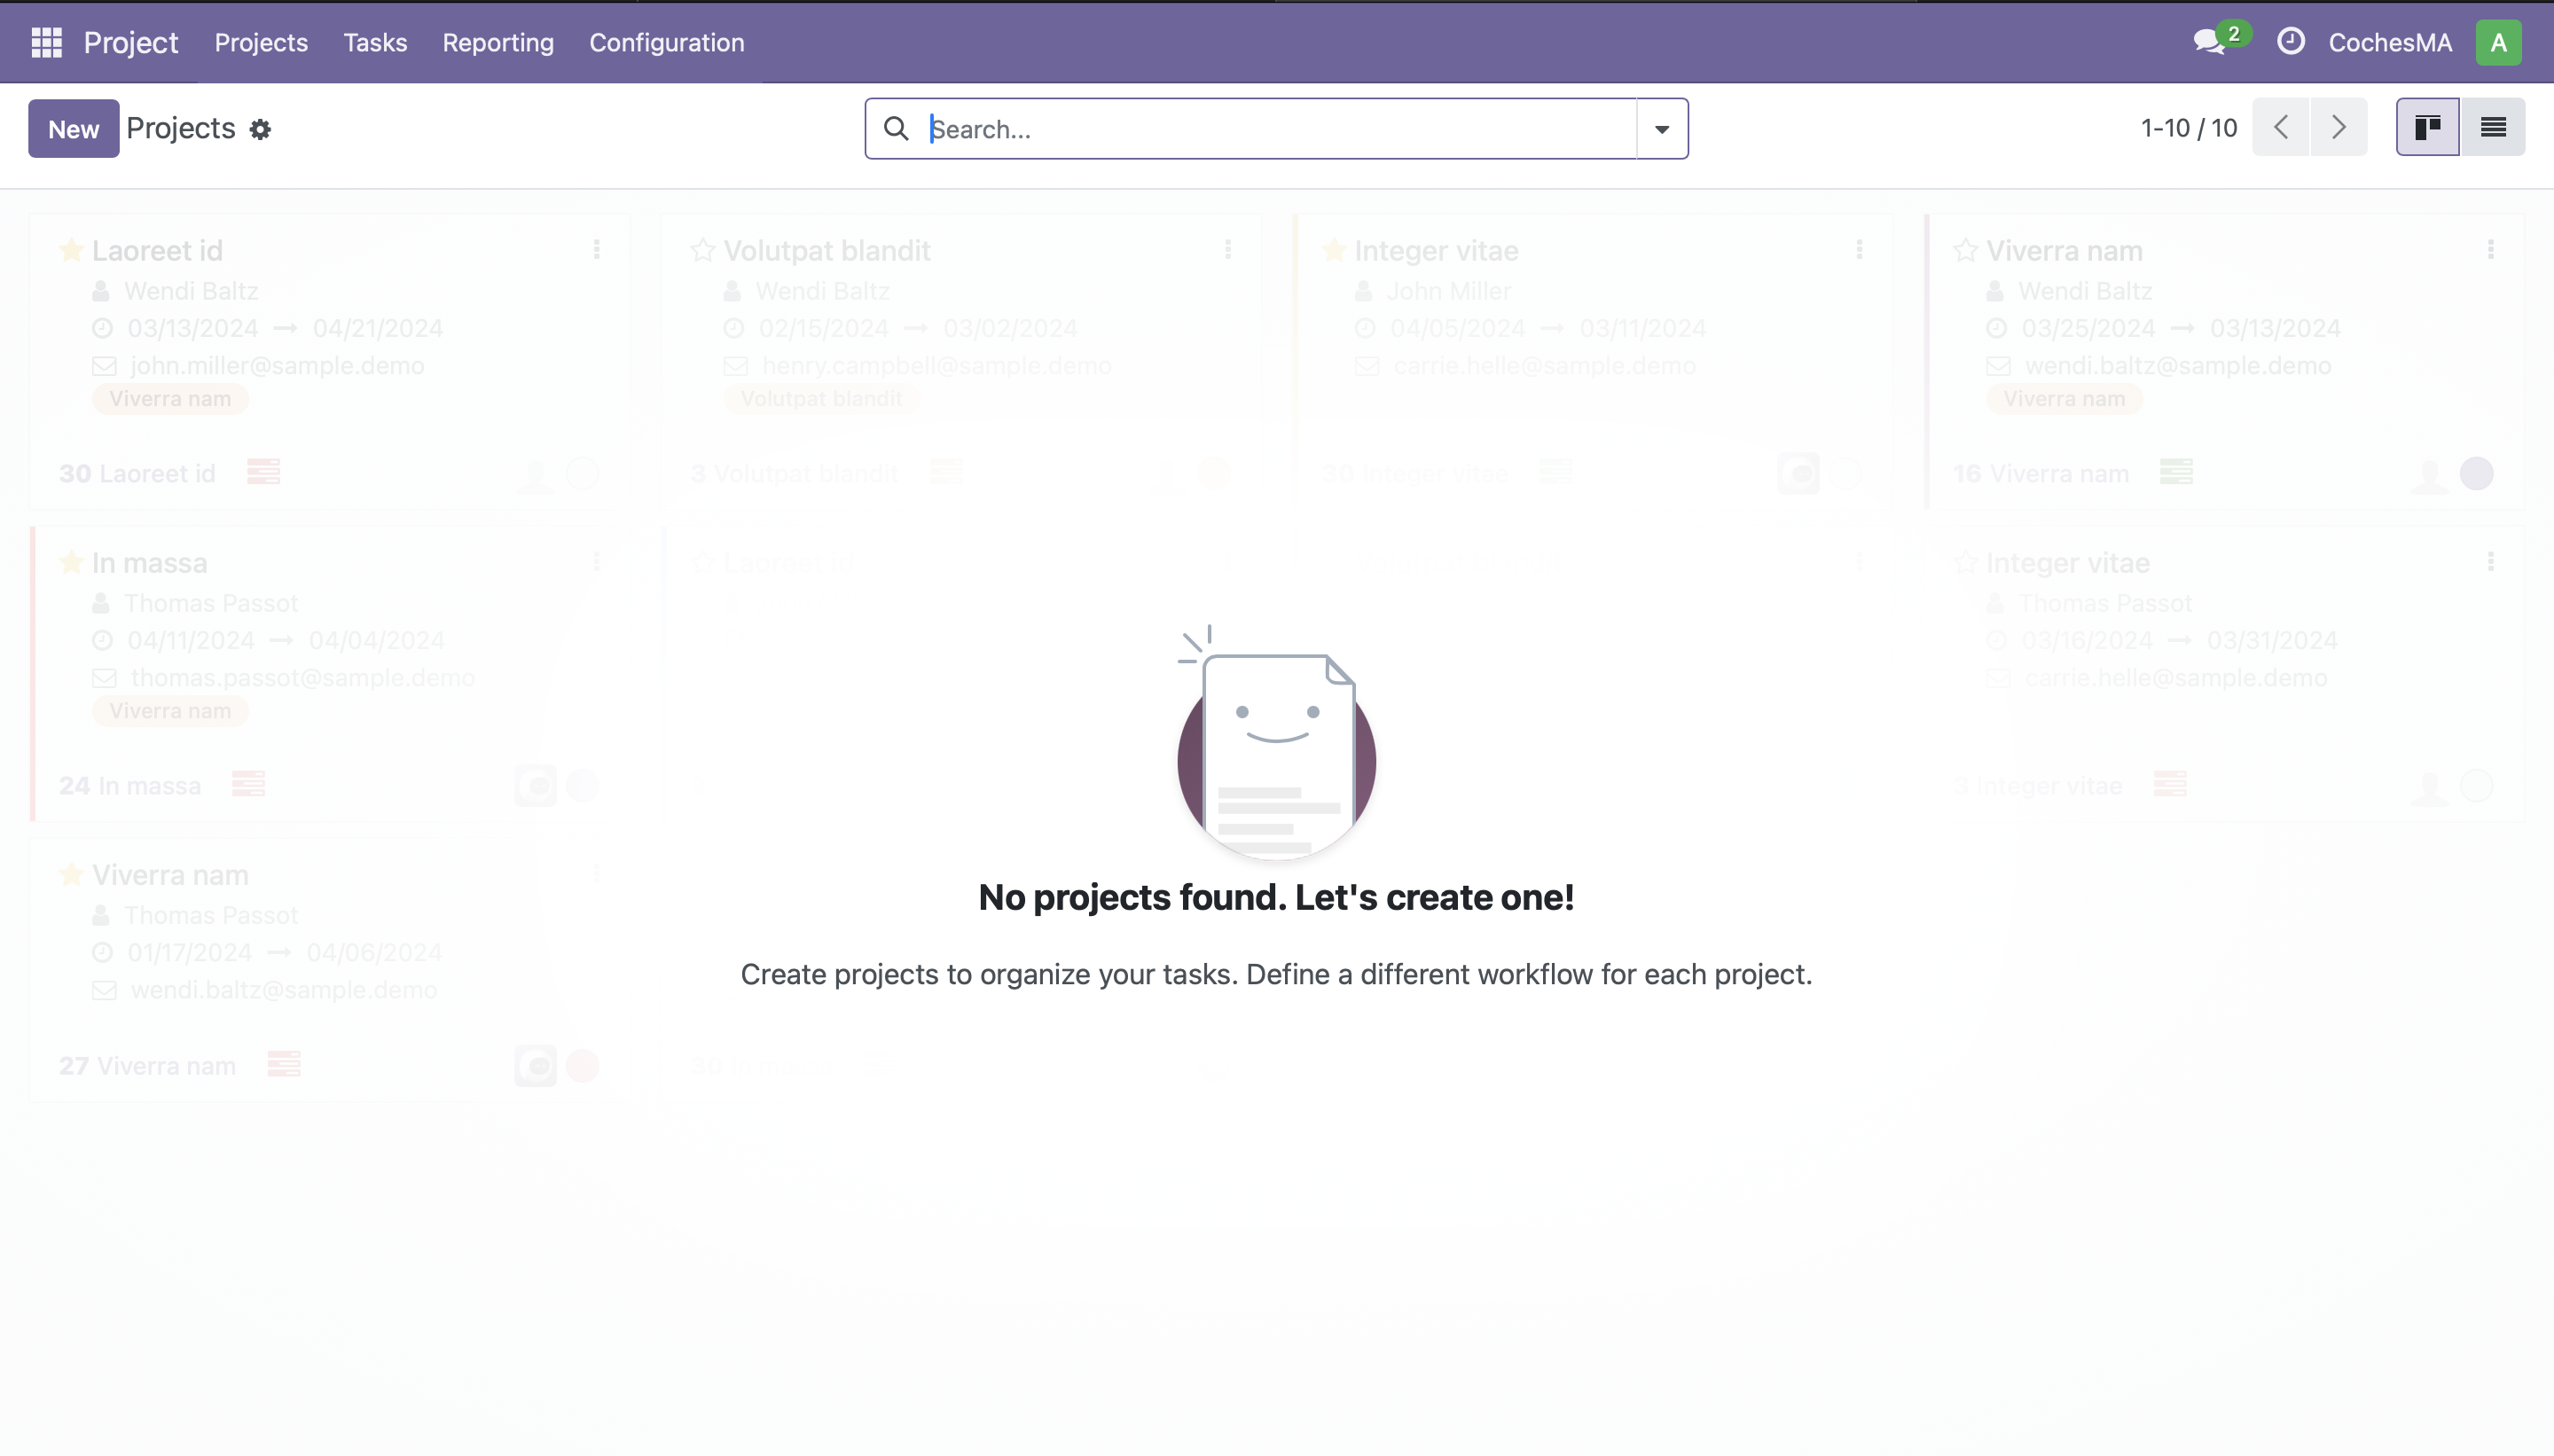
\includegraphics[width=10cm]{emptyProject.png}
    \caption{Página principal del módulo de proyectos.}
    \label{fig:openProyectos}
\end{figure}
 Para crear un nuevo proyecto, pulsa en el botón \textit{New}. Se abrirá un formulario donde se debe introducir la información correspondiente al proyecto que se quiere crear. Una vez introducida la información pulsa en \textit{Create project} y se creará el proyecto.
\begin{figure}[h]
    \centering
    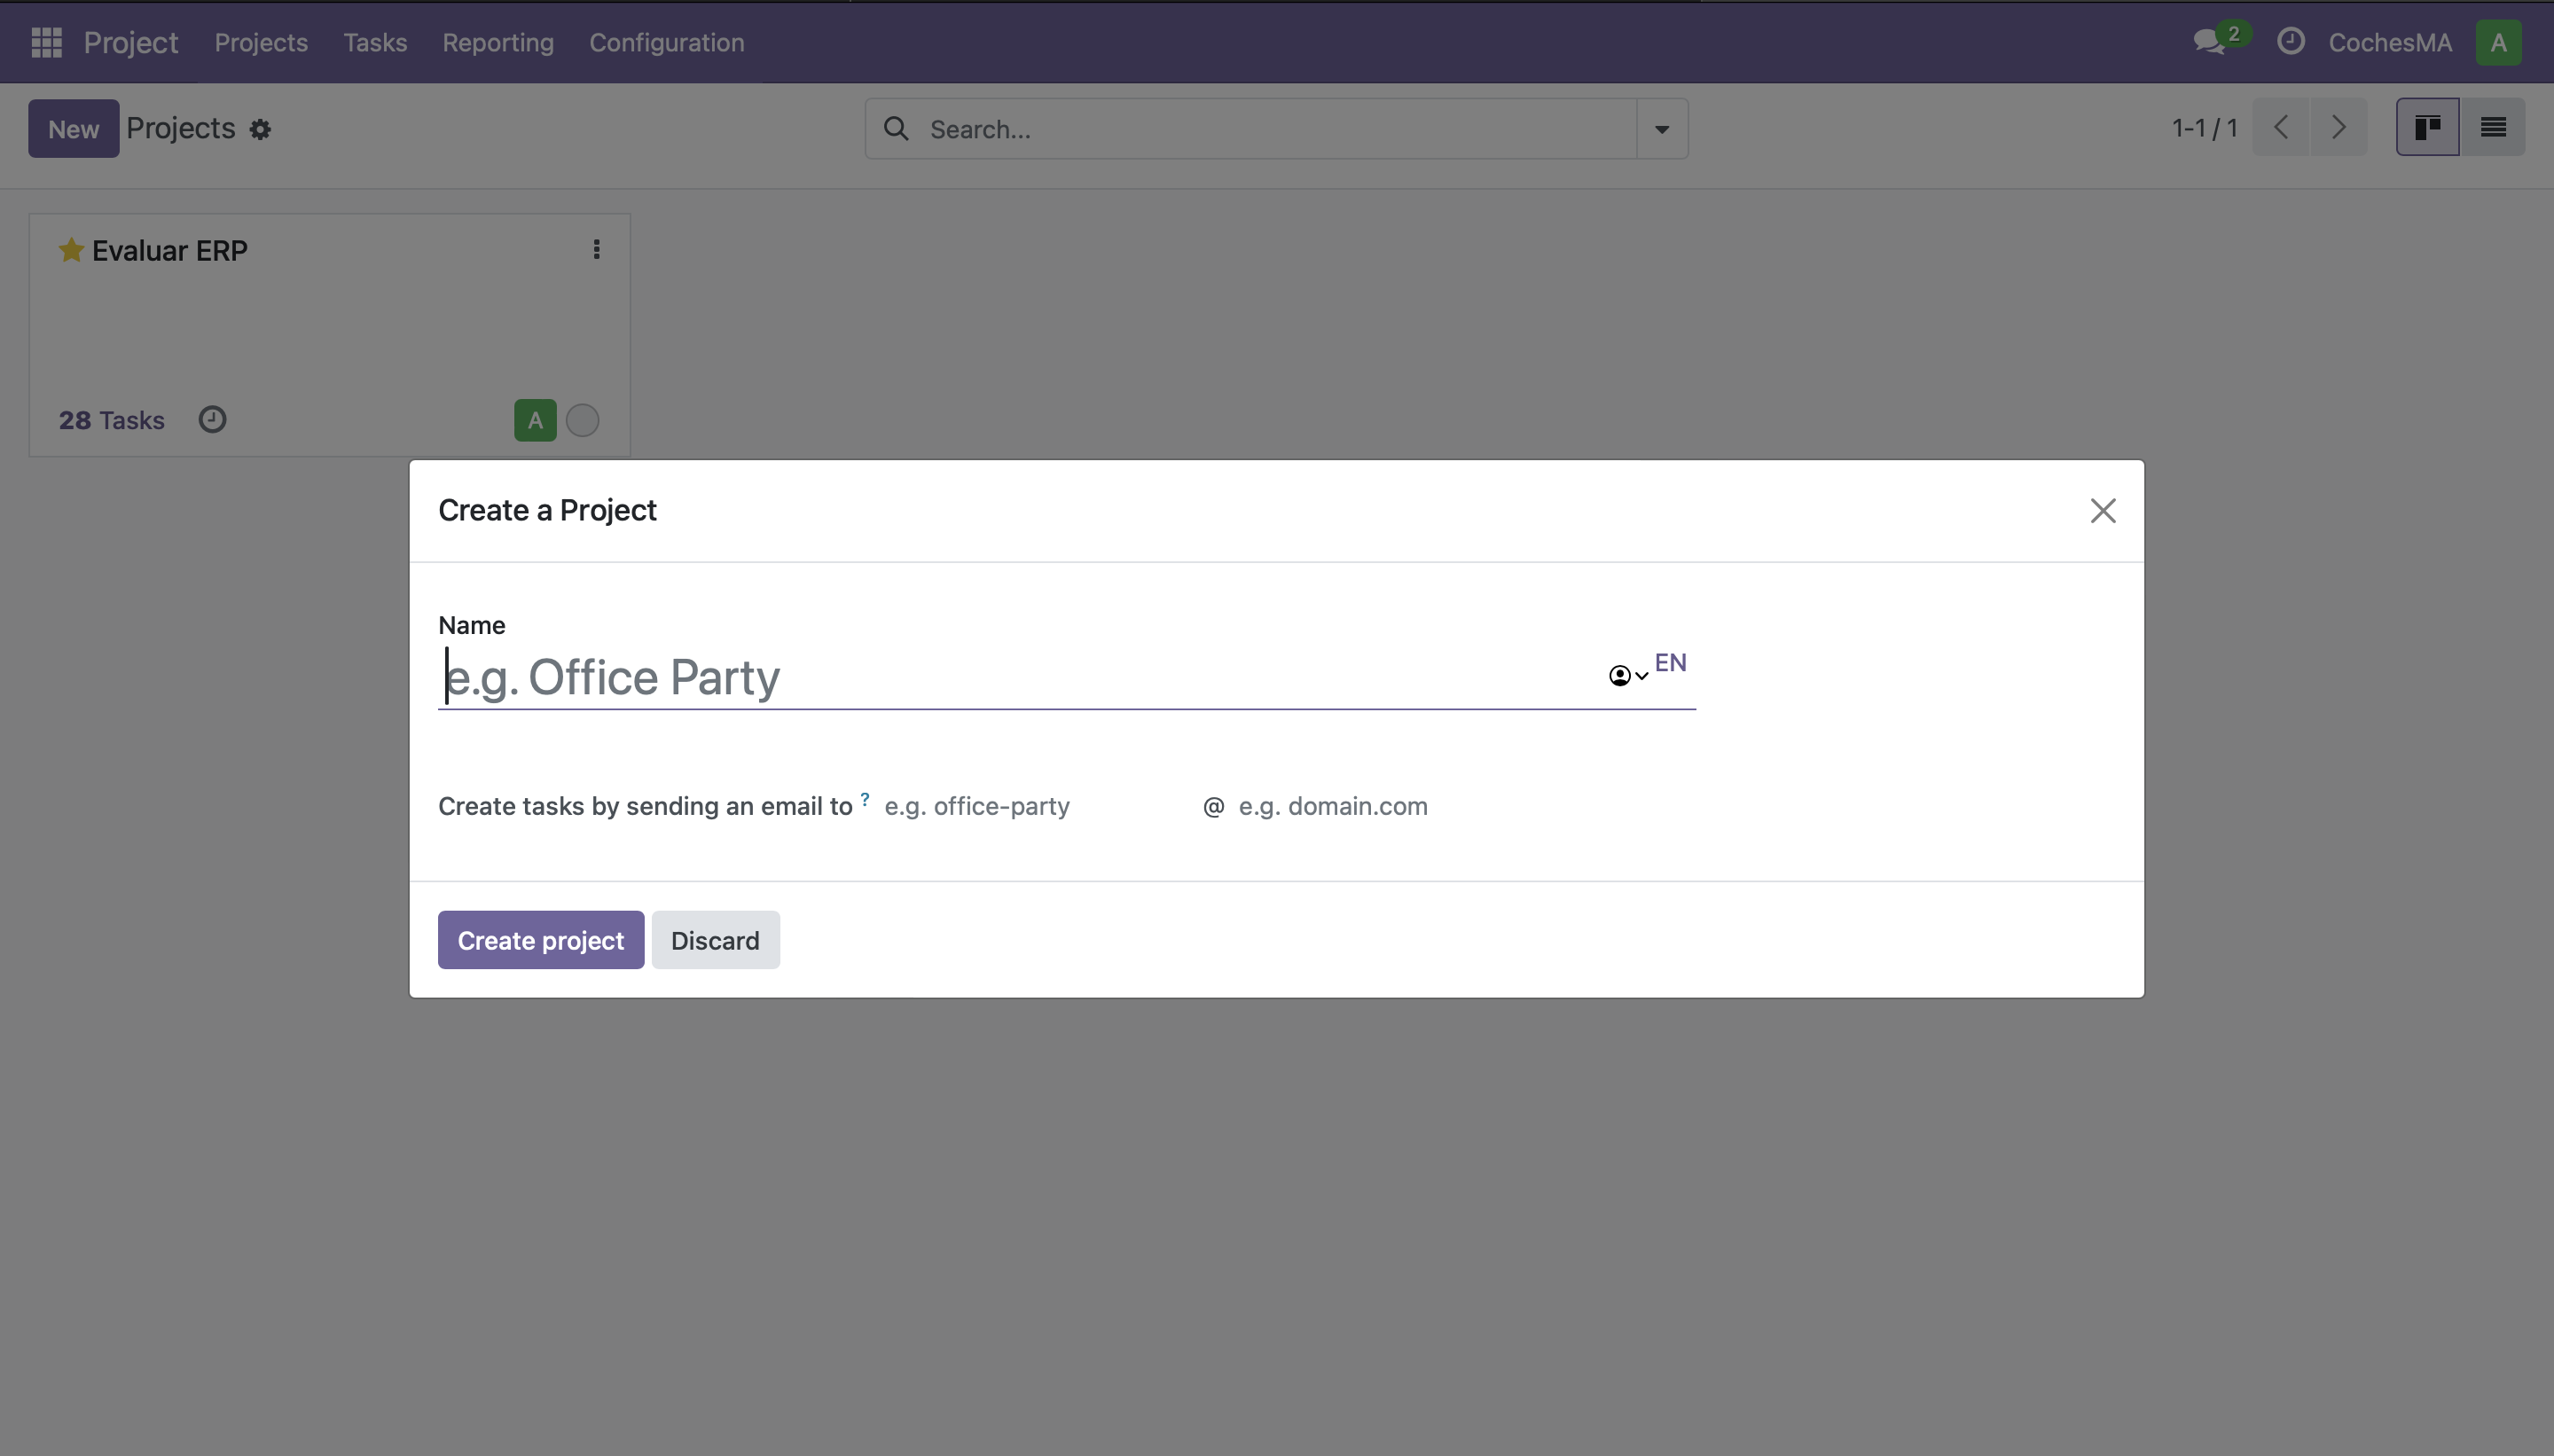
\includegraphics[width=10cm]{addProject.png}
    \caption{Crear un nuevo proyecto.}
    \label{fig:openProyectos}
\end{figure}
\newpage
\paragraph{}
Una vez que hemos creado el primer proyecto, se nos abrirá automáticamente la página de este proyecto. Lo primero que debemos hacer para poder comenzar a gestionar nuestro proyecto es crear las columnas para clasificar nuestras tareas. En este caso hemos decidido dividir en tres estados: Pendiente, En proceso y Hecho. Para crear las columnas hay que pulsar en el botón \textit{+Stage}, introducir el nombre de la columna y pulsar en \textit{Add}.
\begin{figure}[h]
    \centering
    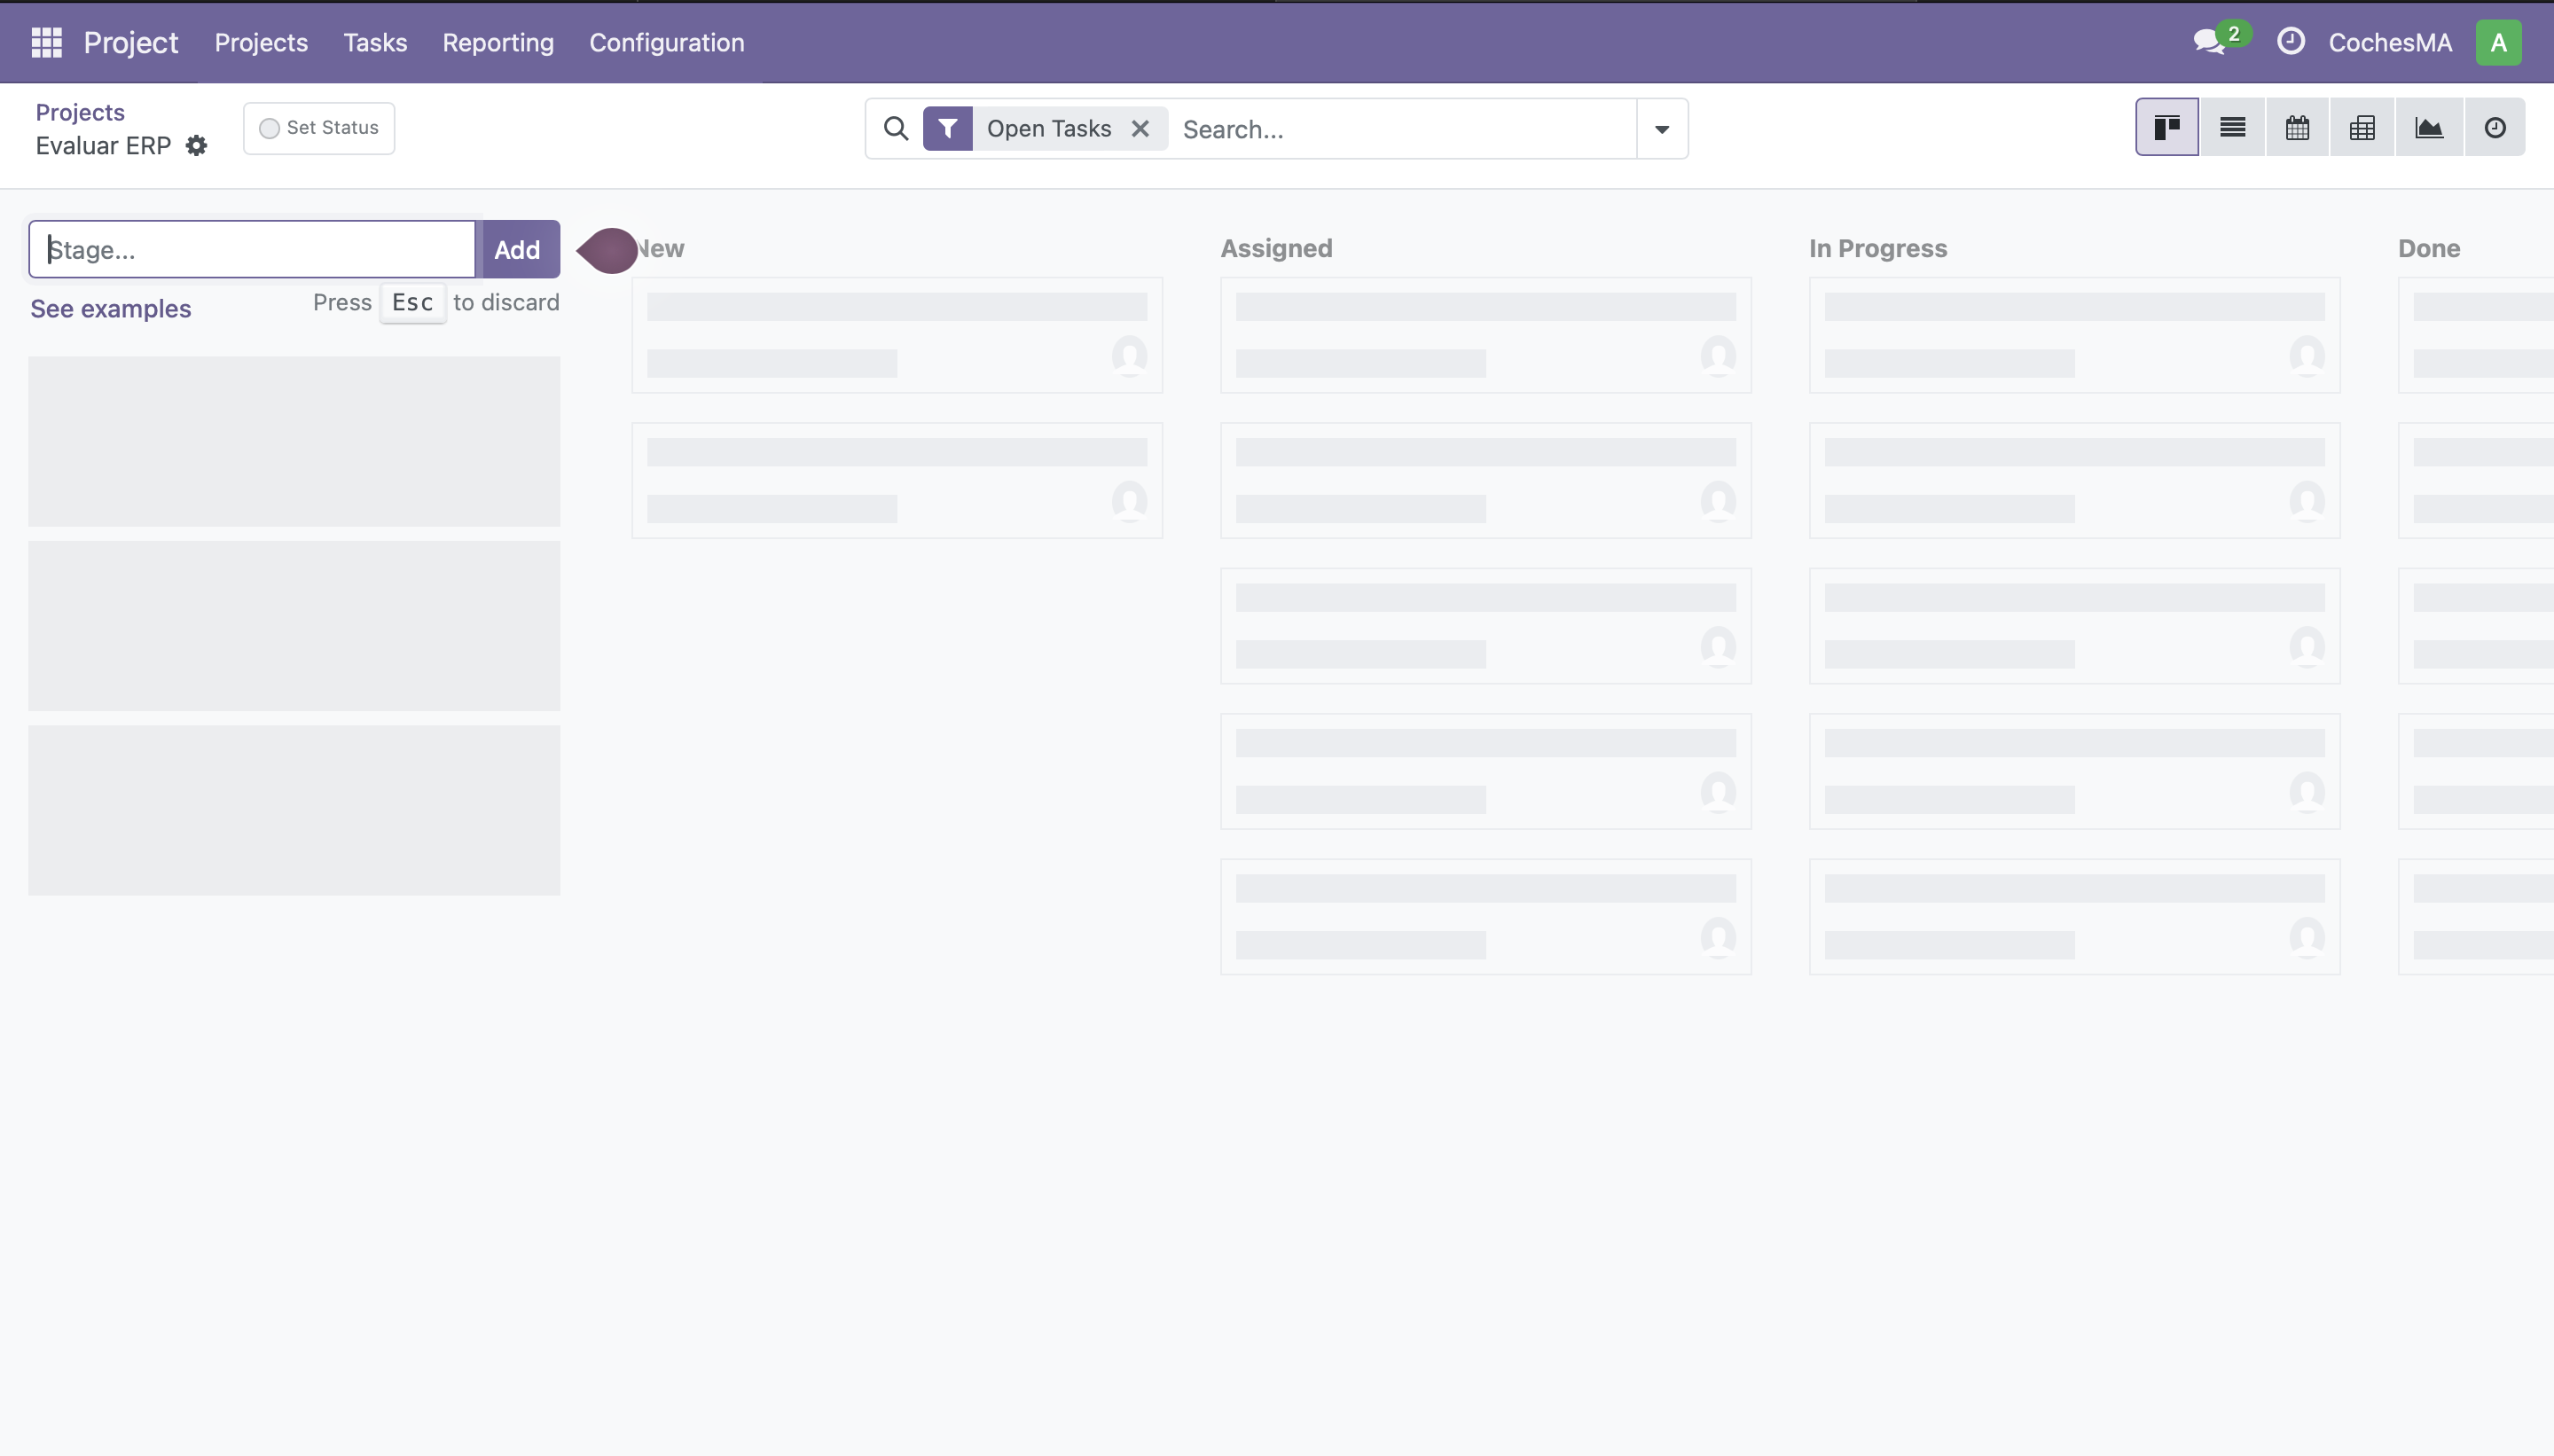
\includegraphics[width=10cm]{addColProject.png}
    \caption{Añadir columnas.}
    \label{fig:openProyectos}
\end{figure}
\begin{figure}[h]
    \centering
    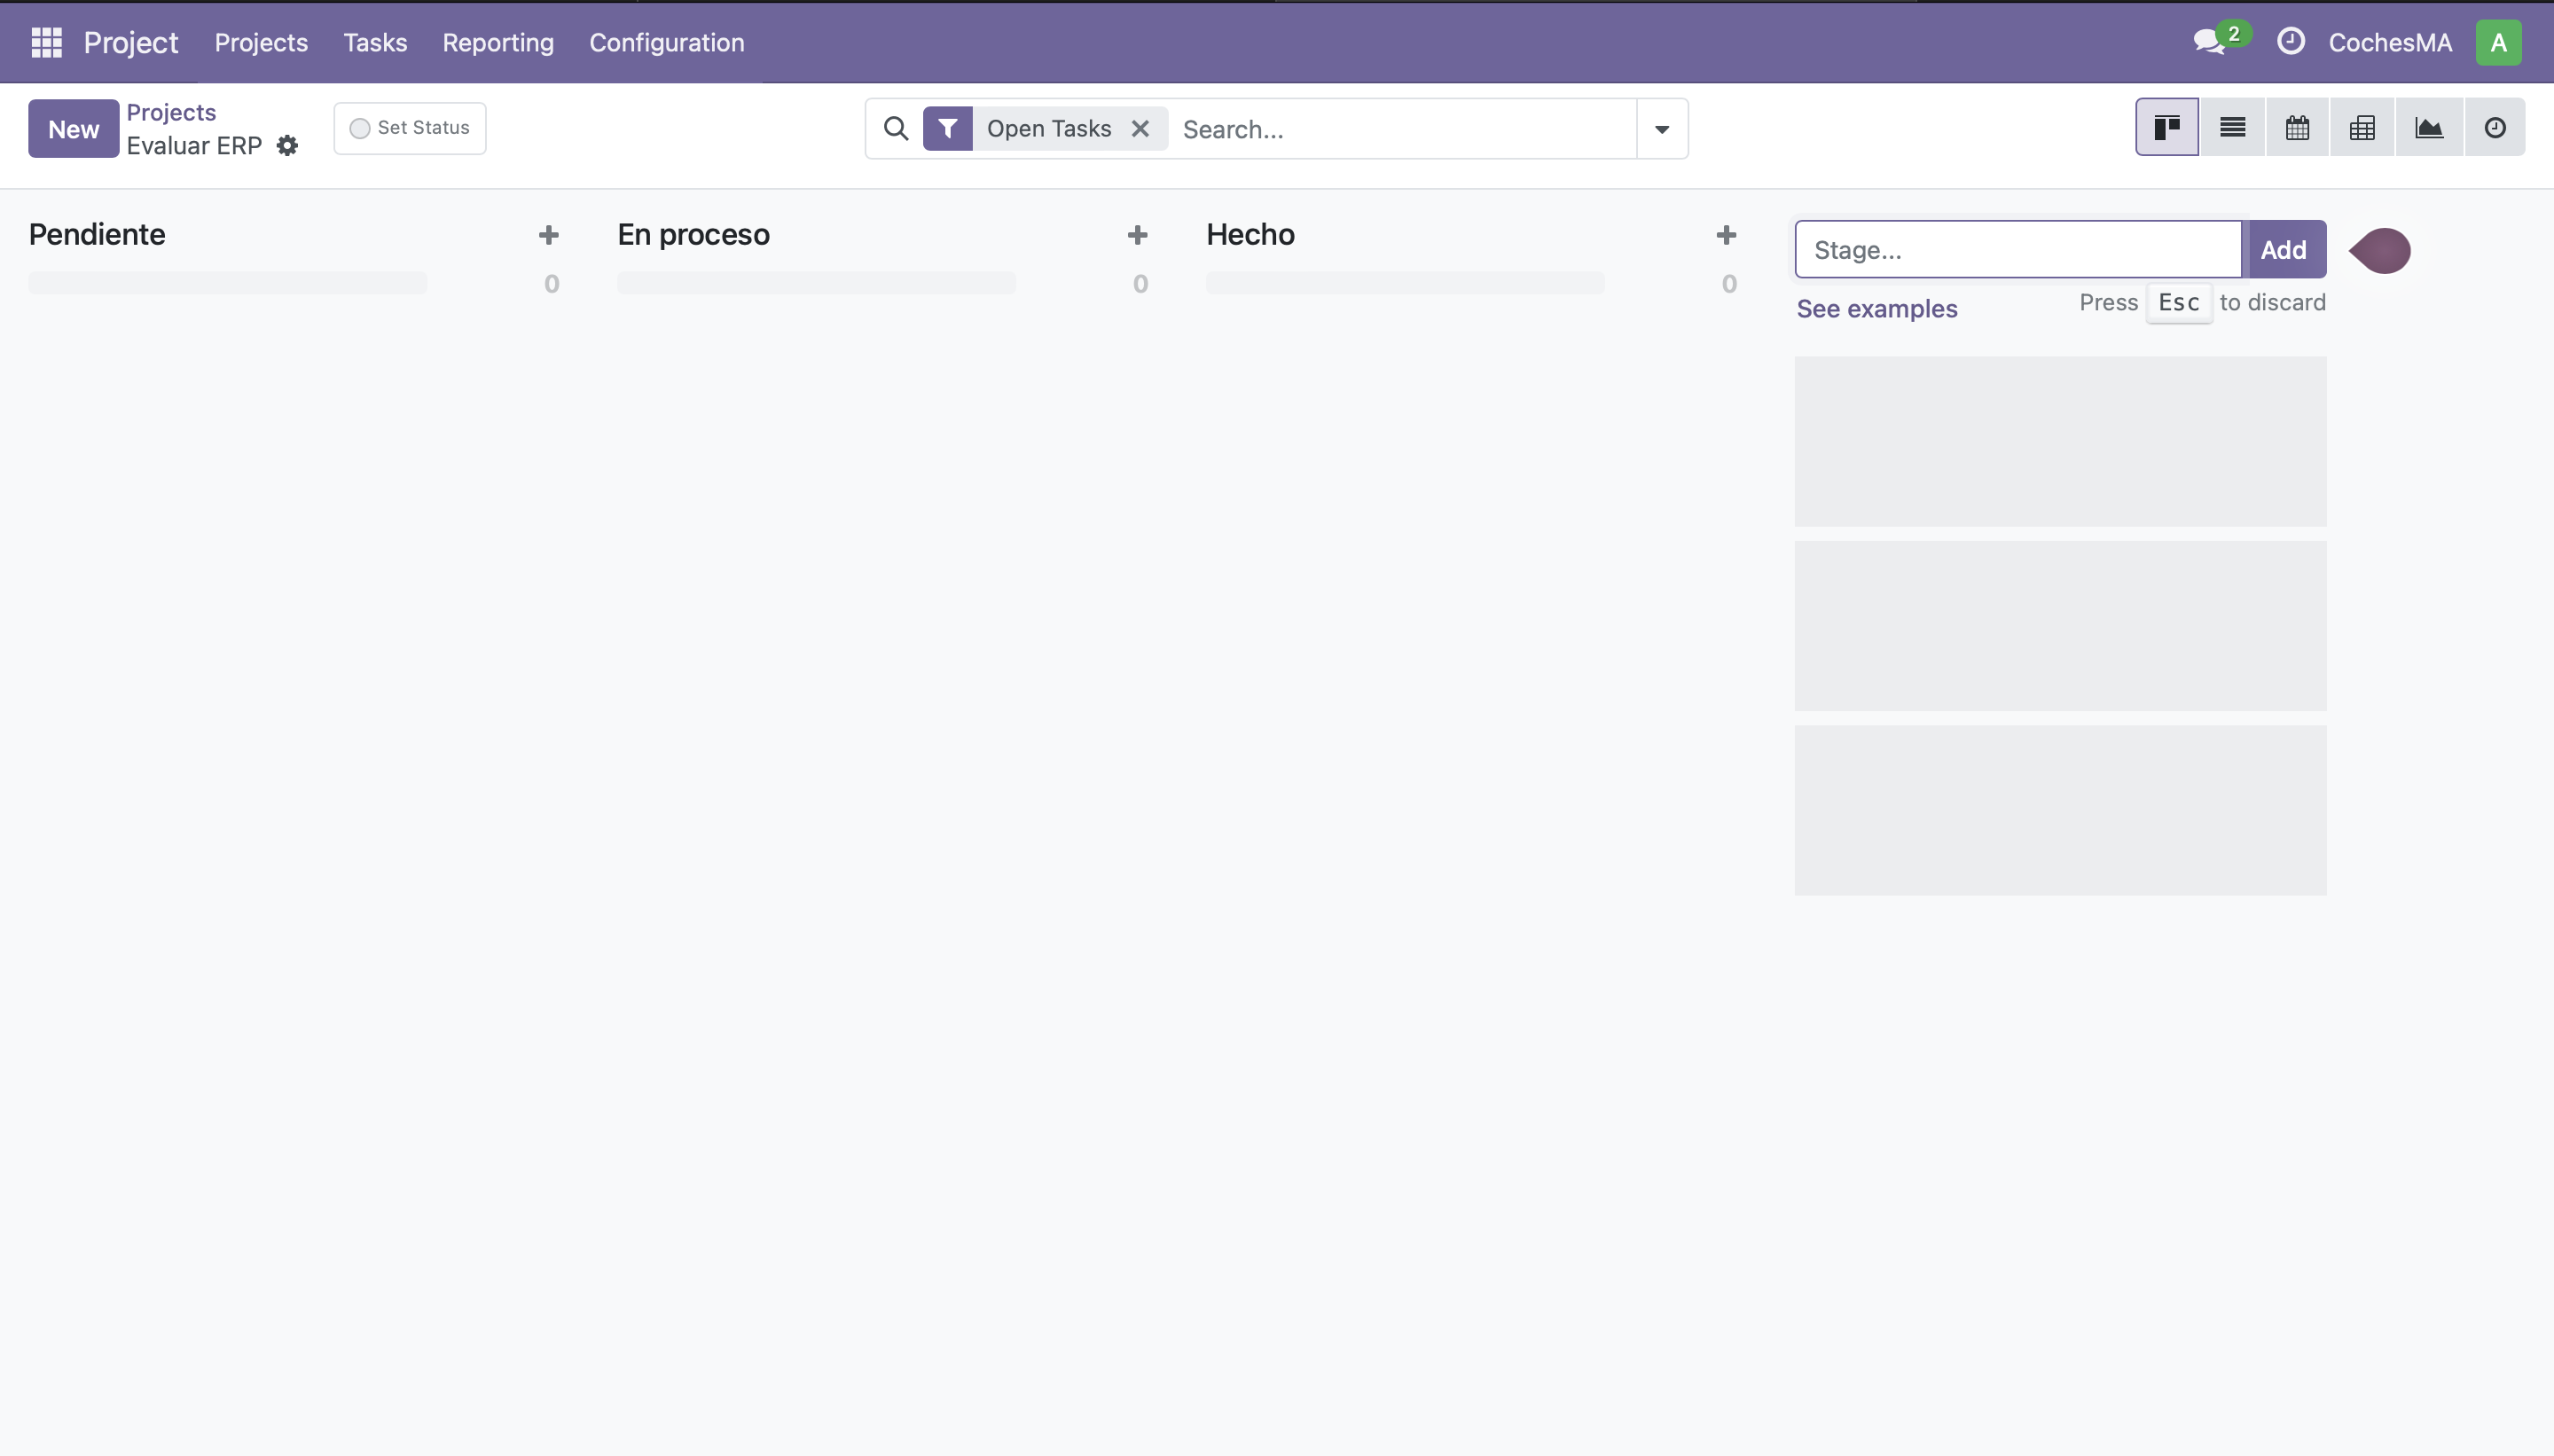
\includegraphics[width=10cm]{colsAddedProject.png}
    \caption{Columnas añadidas.}
    \label{fig:openProyectos}
\end{figure}
\paragraph{}
Tras crear las columnas, podemos añadir tareas a nuestro proyecto. Para ello, pulsa en el botón \textit{+}, introduce la información correspondiente a la tarea que se quiere añadir y pulsa en \textit{Add}. Las tareas están formadas por un título, una descripción, si son prioritarias (estrella) y las personas que deben realizarla. Además, se pueden añadir sub-tareas y las tareas que la bloquean.
\begin{figure}[h]
    \centering
    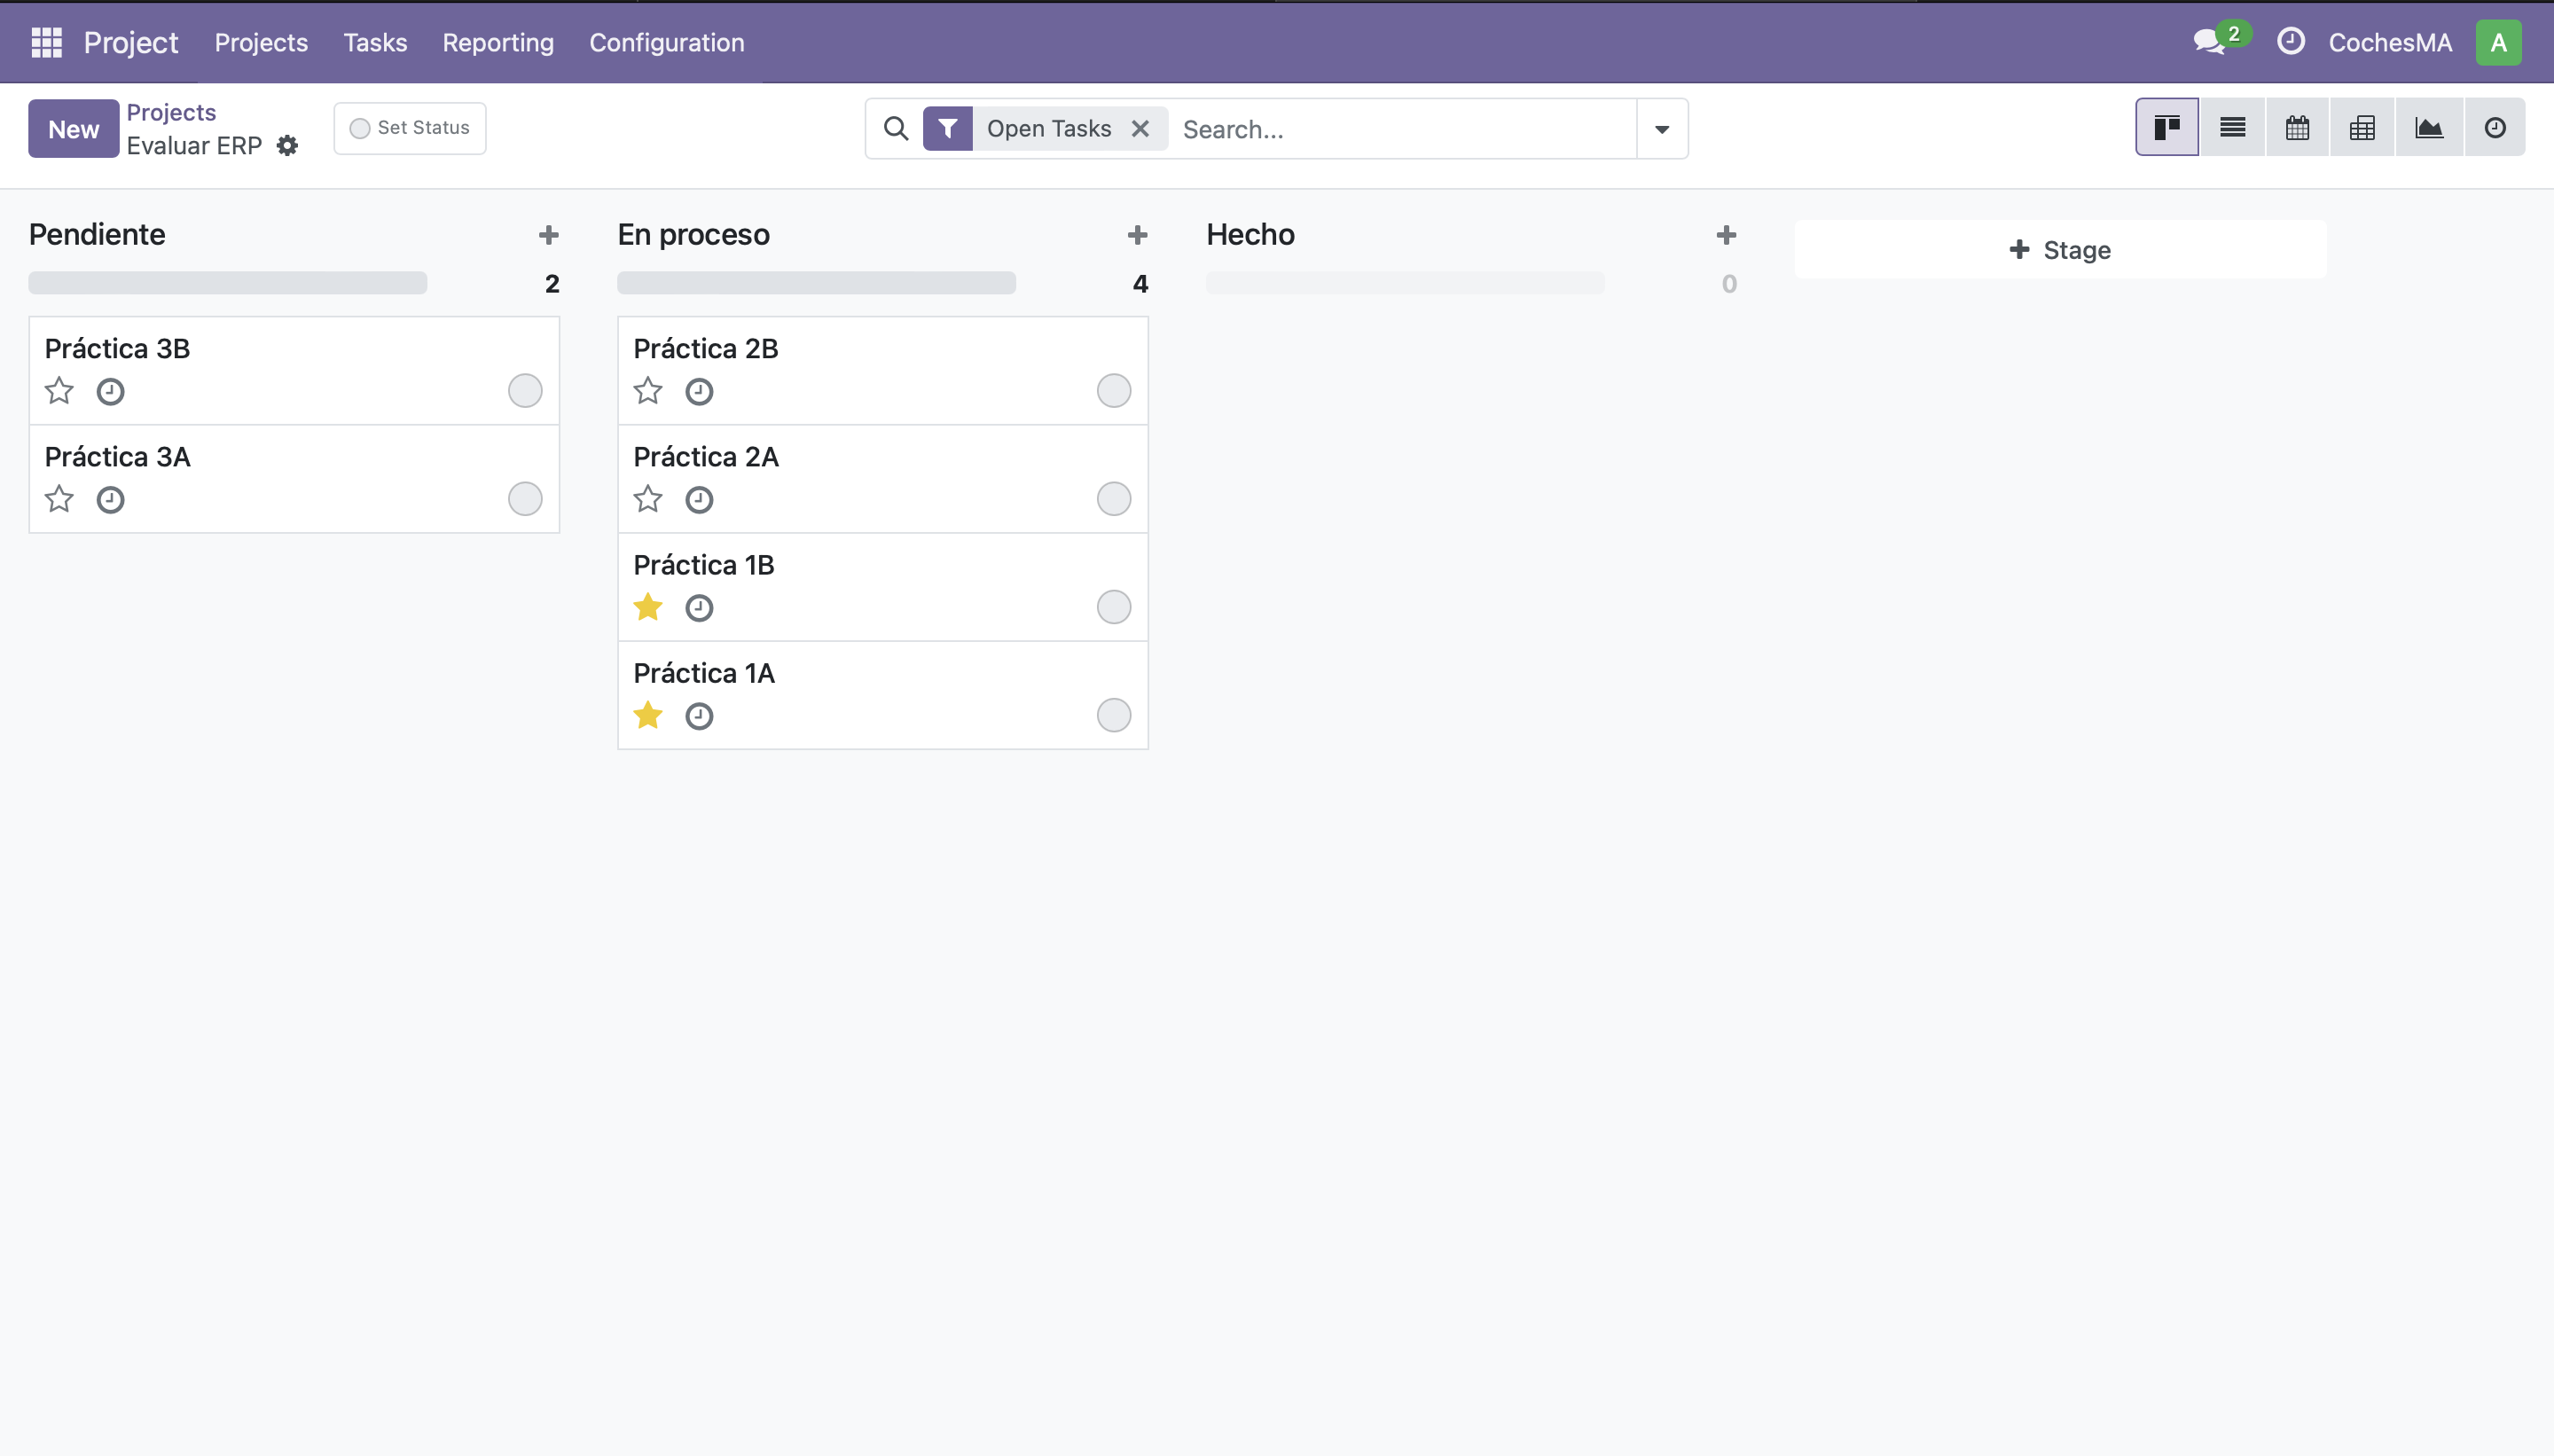
\includegraphics[width=10cm]{itemsAddedProject.png}
    \caption{Items añadidos.}
    \label{fig:openProyectos}
\end{figure}
\newpage
\subsection{Asignación de tareas}
\paragraph{}
Para asignar una tarea a alguien se puede hacer al crear la tarea o desde la tarea. En ambos casos se debe seleccionar la persona que se quiere que realice la tarea. Por ejemplo, en este caso hemos asignado la tare \textit{Práctica 1A} a Marcus, uno de los integrantes de la empresa y la tarea \textit{Práctica 1B} a James, otro integrante de la empresa.
\begin{figure}[h]
    \centering
    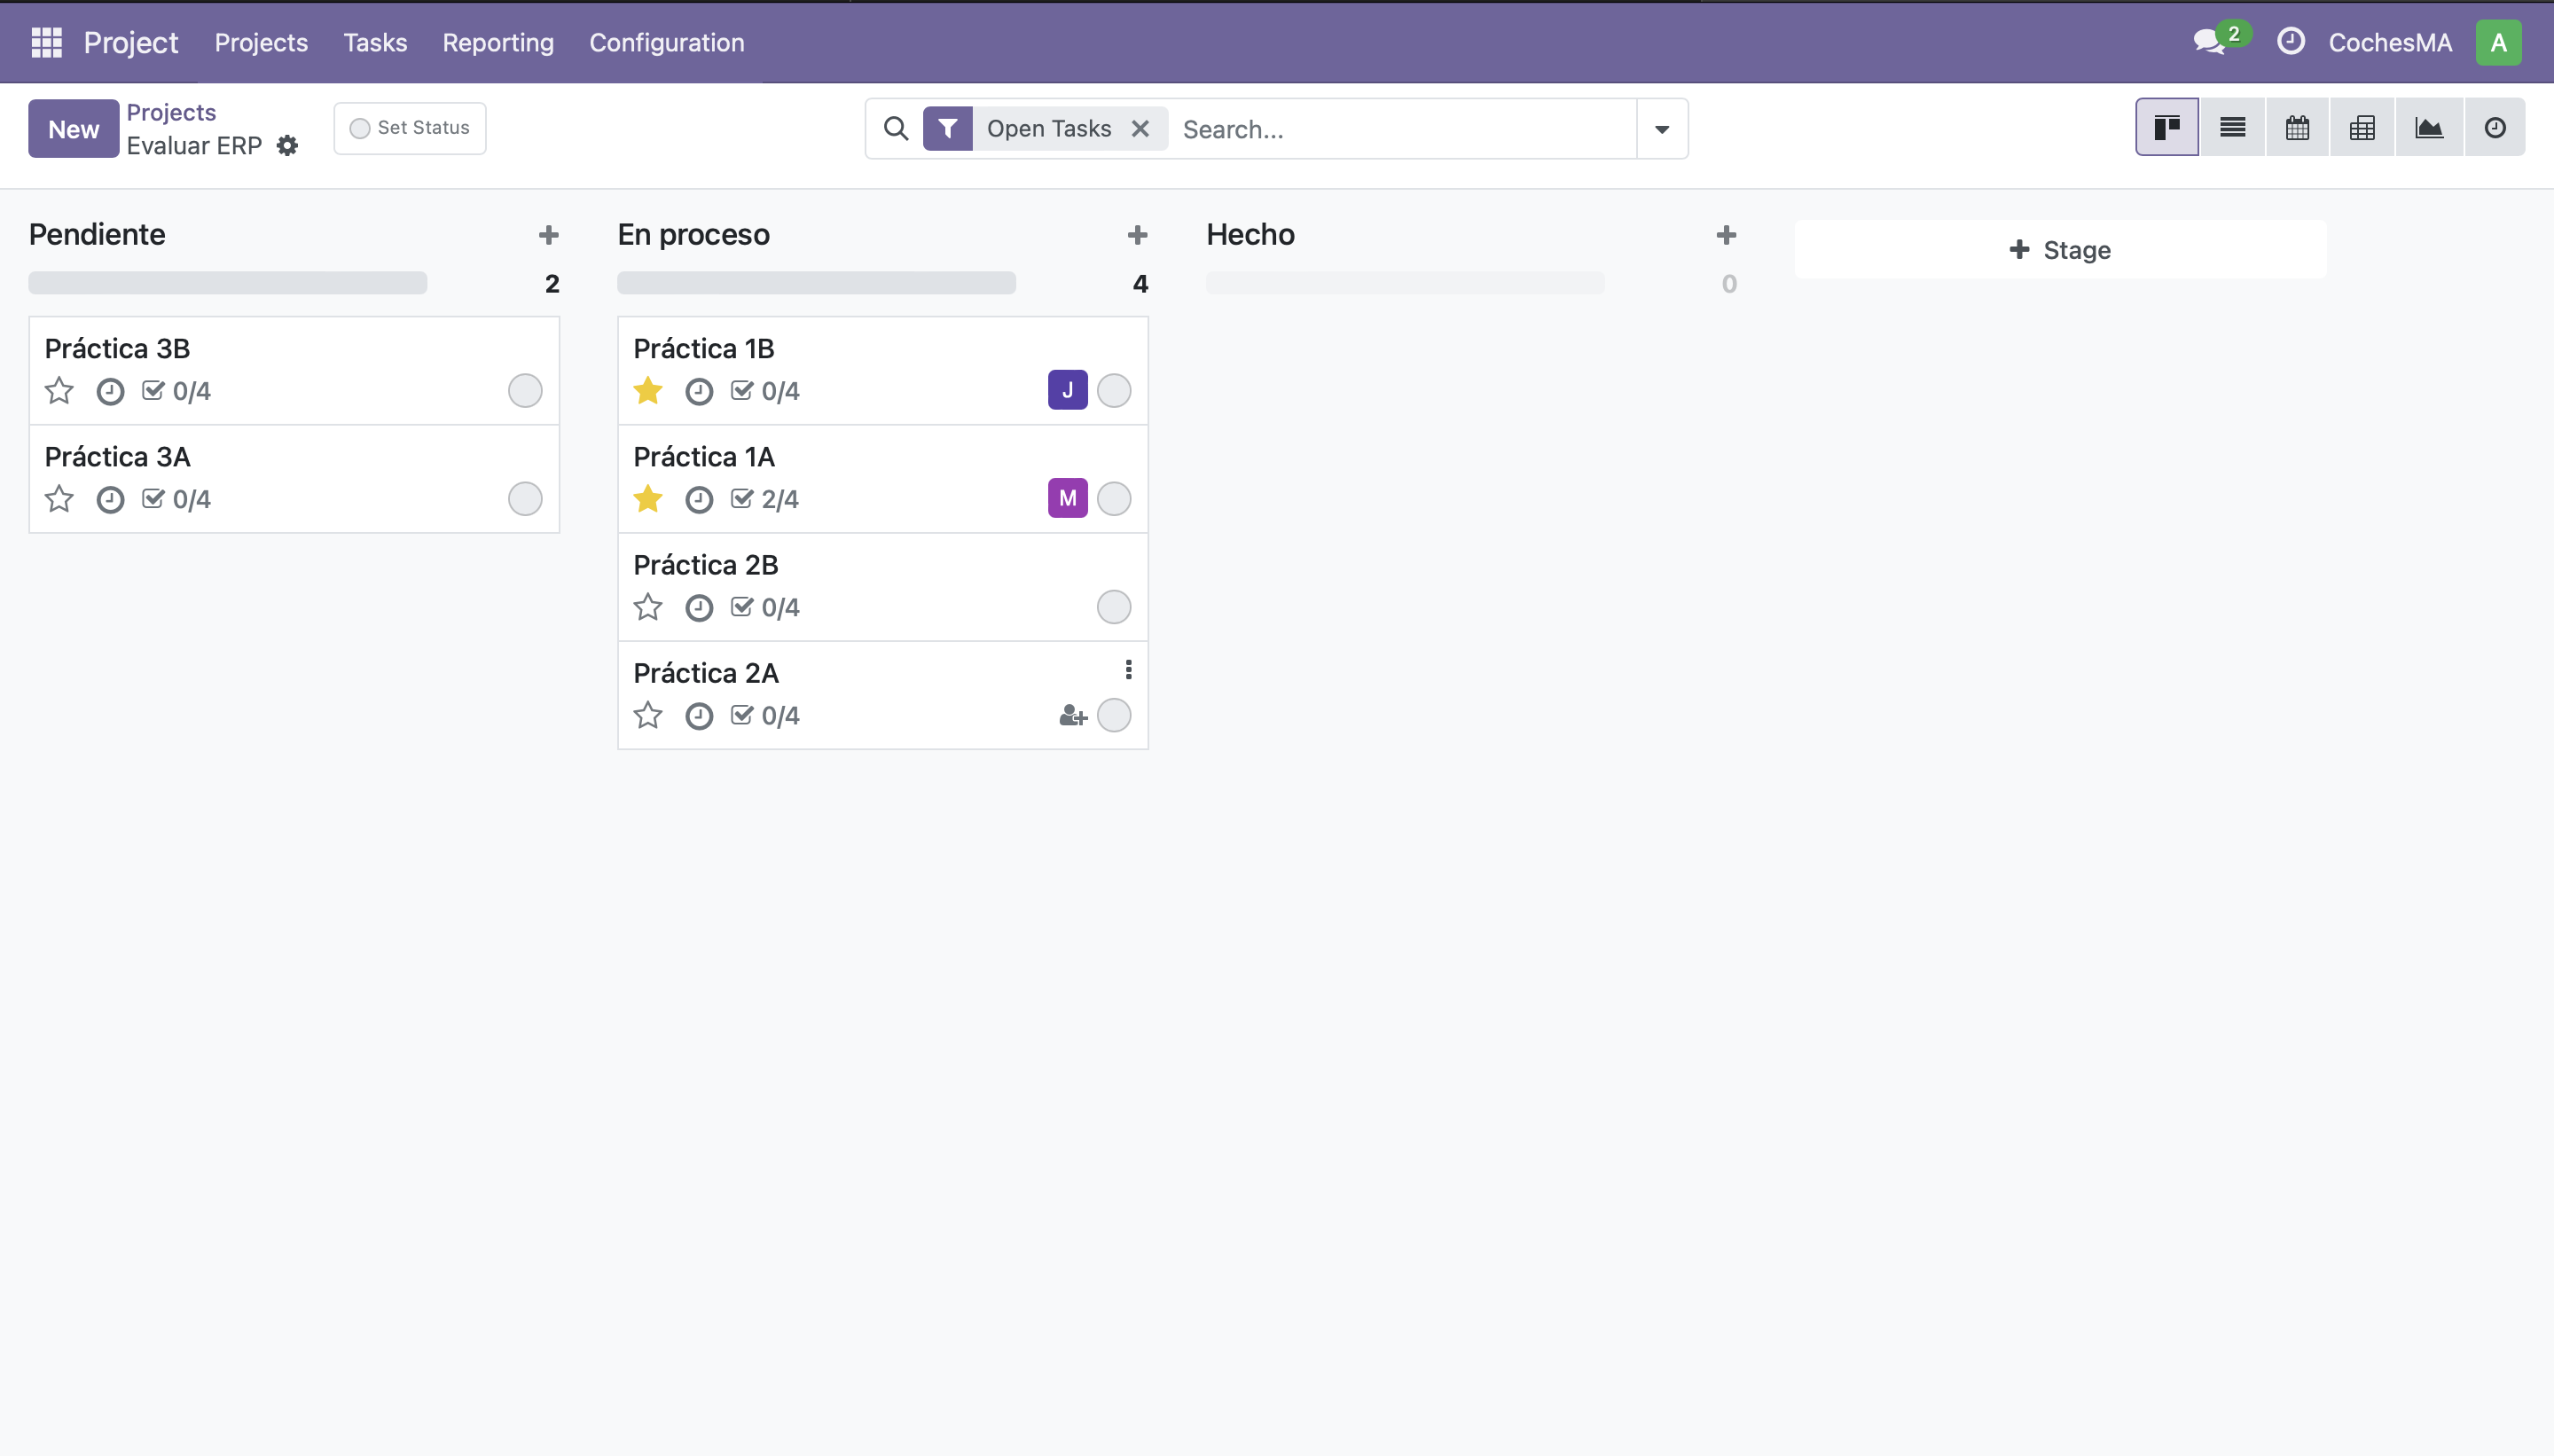
\includegraphics[width=10cm]{assignProject.png}
    \caption{Asignación tarea.}
    \label{fig:openProyectos}
\end{figure}
\newpage
\subsection{Sub-tareas}
\paragraph{}
Cada tarea puede estar formada por otras tareas más pequeñas. Para añadir una sub-tarea a una tarea, pulsa en la tarea y se abrirá la página de la tarea. Selecciona la opción \textit{Add a sub-task} y añade las correspondientes sub-tareas. En este caso hemos añadido 4 sub-tareas a la tarea \textit{Práctica 1A}, las tareas correspondientes a cada una de las partes de la práctica. Además se pueden marcar como completadas y asignar a una persona.
\begin{figure}[h]
    \centering
    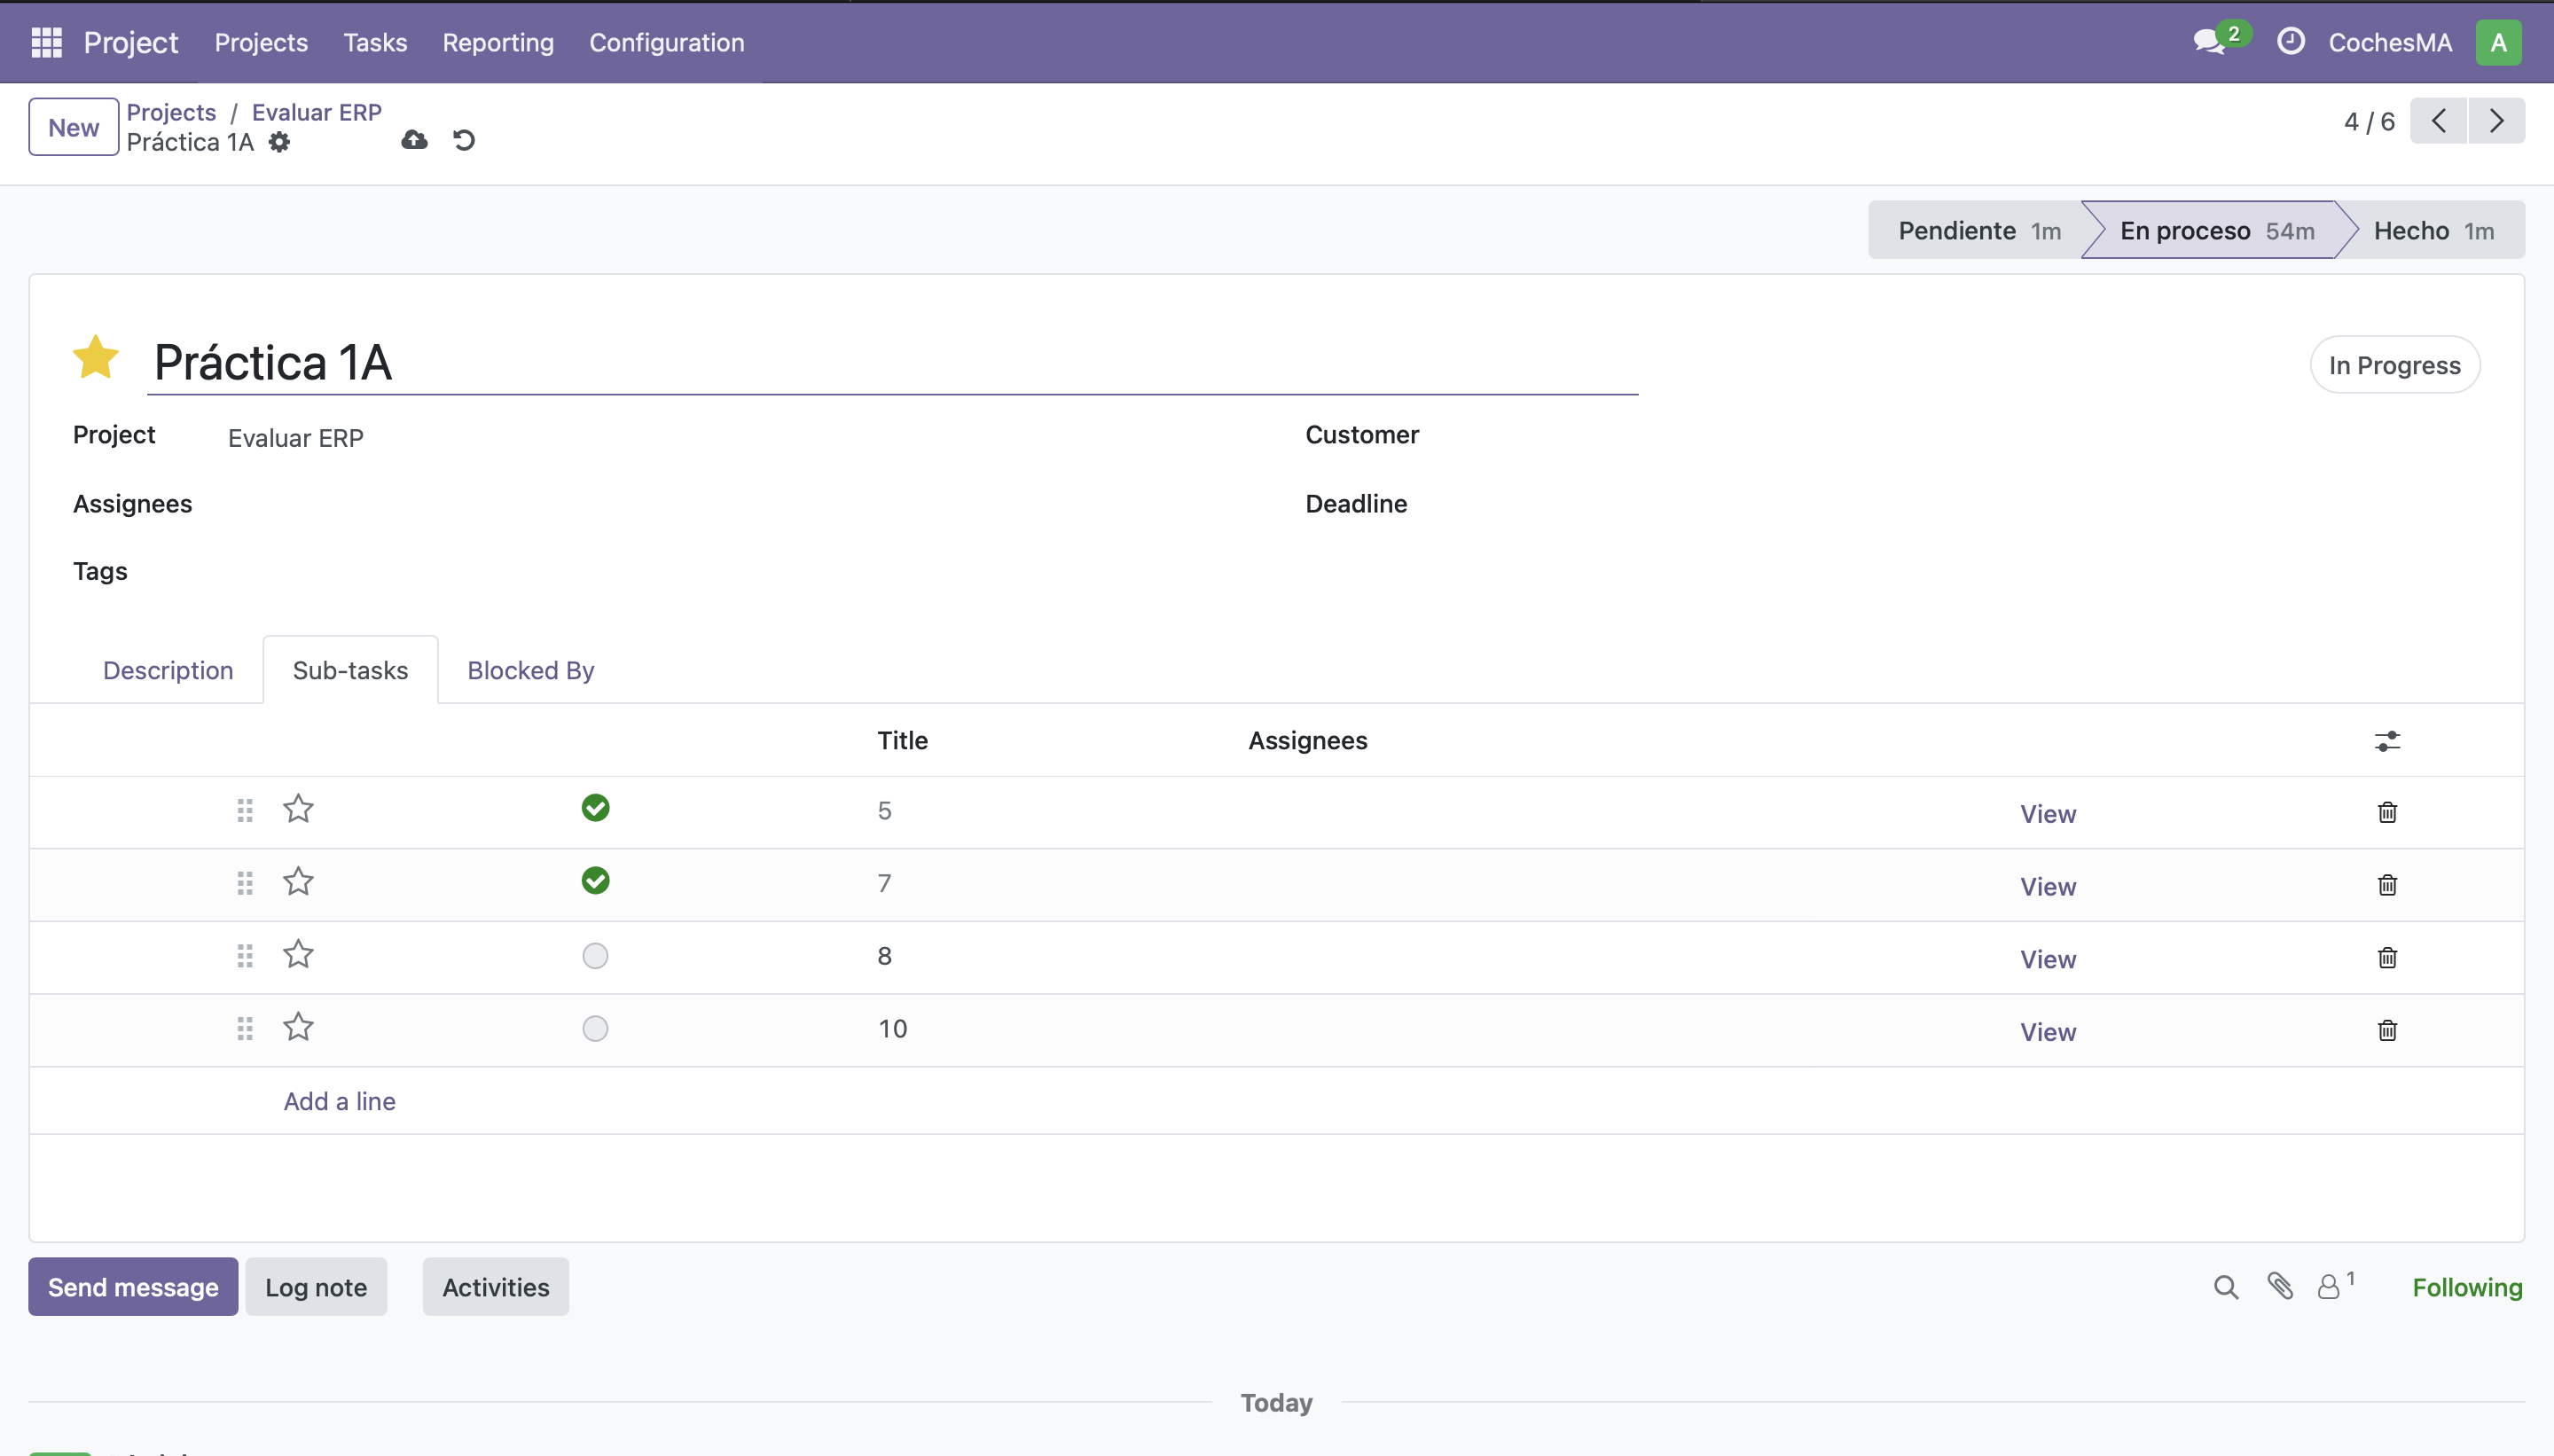
\includegraphics[width=10cm]{subItemsProject.png}
    \caption{Sub-tareas.}
    \label{fig:openProyectos}
\end{figure}
\begin{figure}[h]
    \centering
    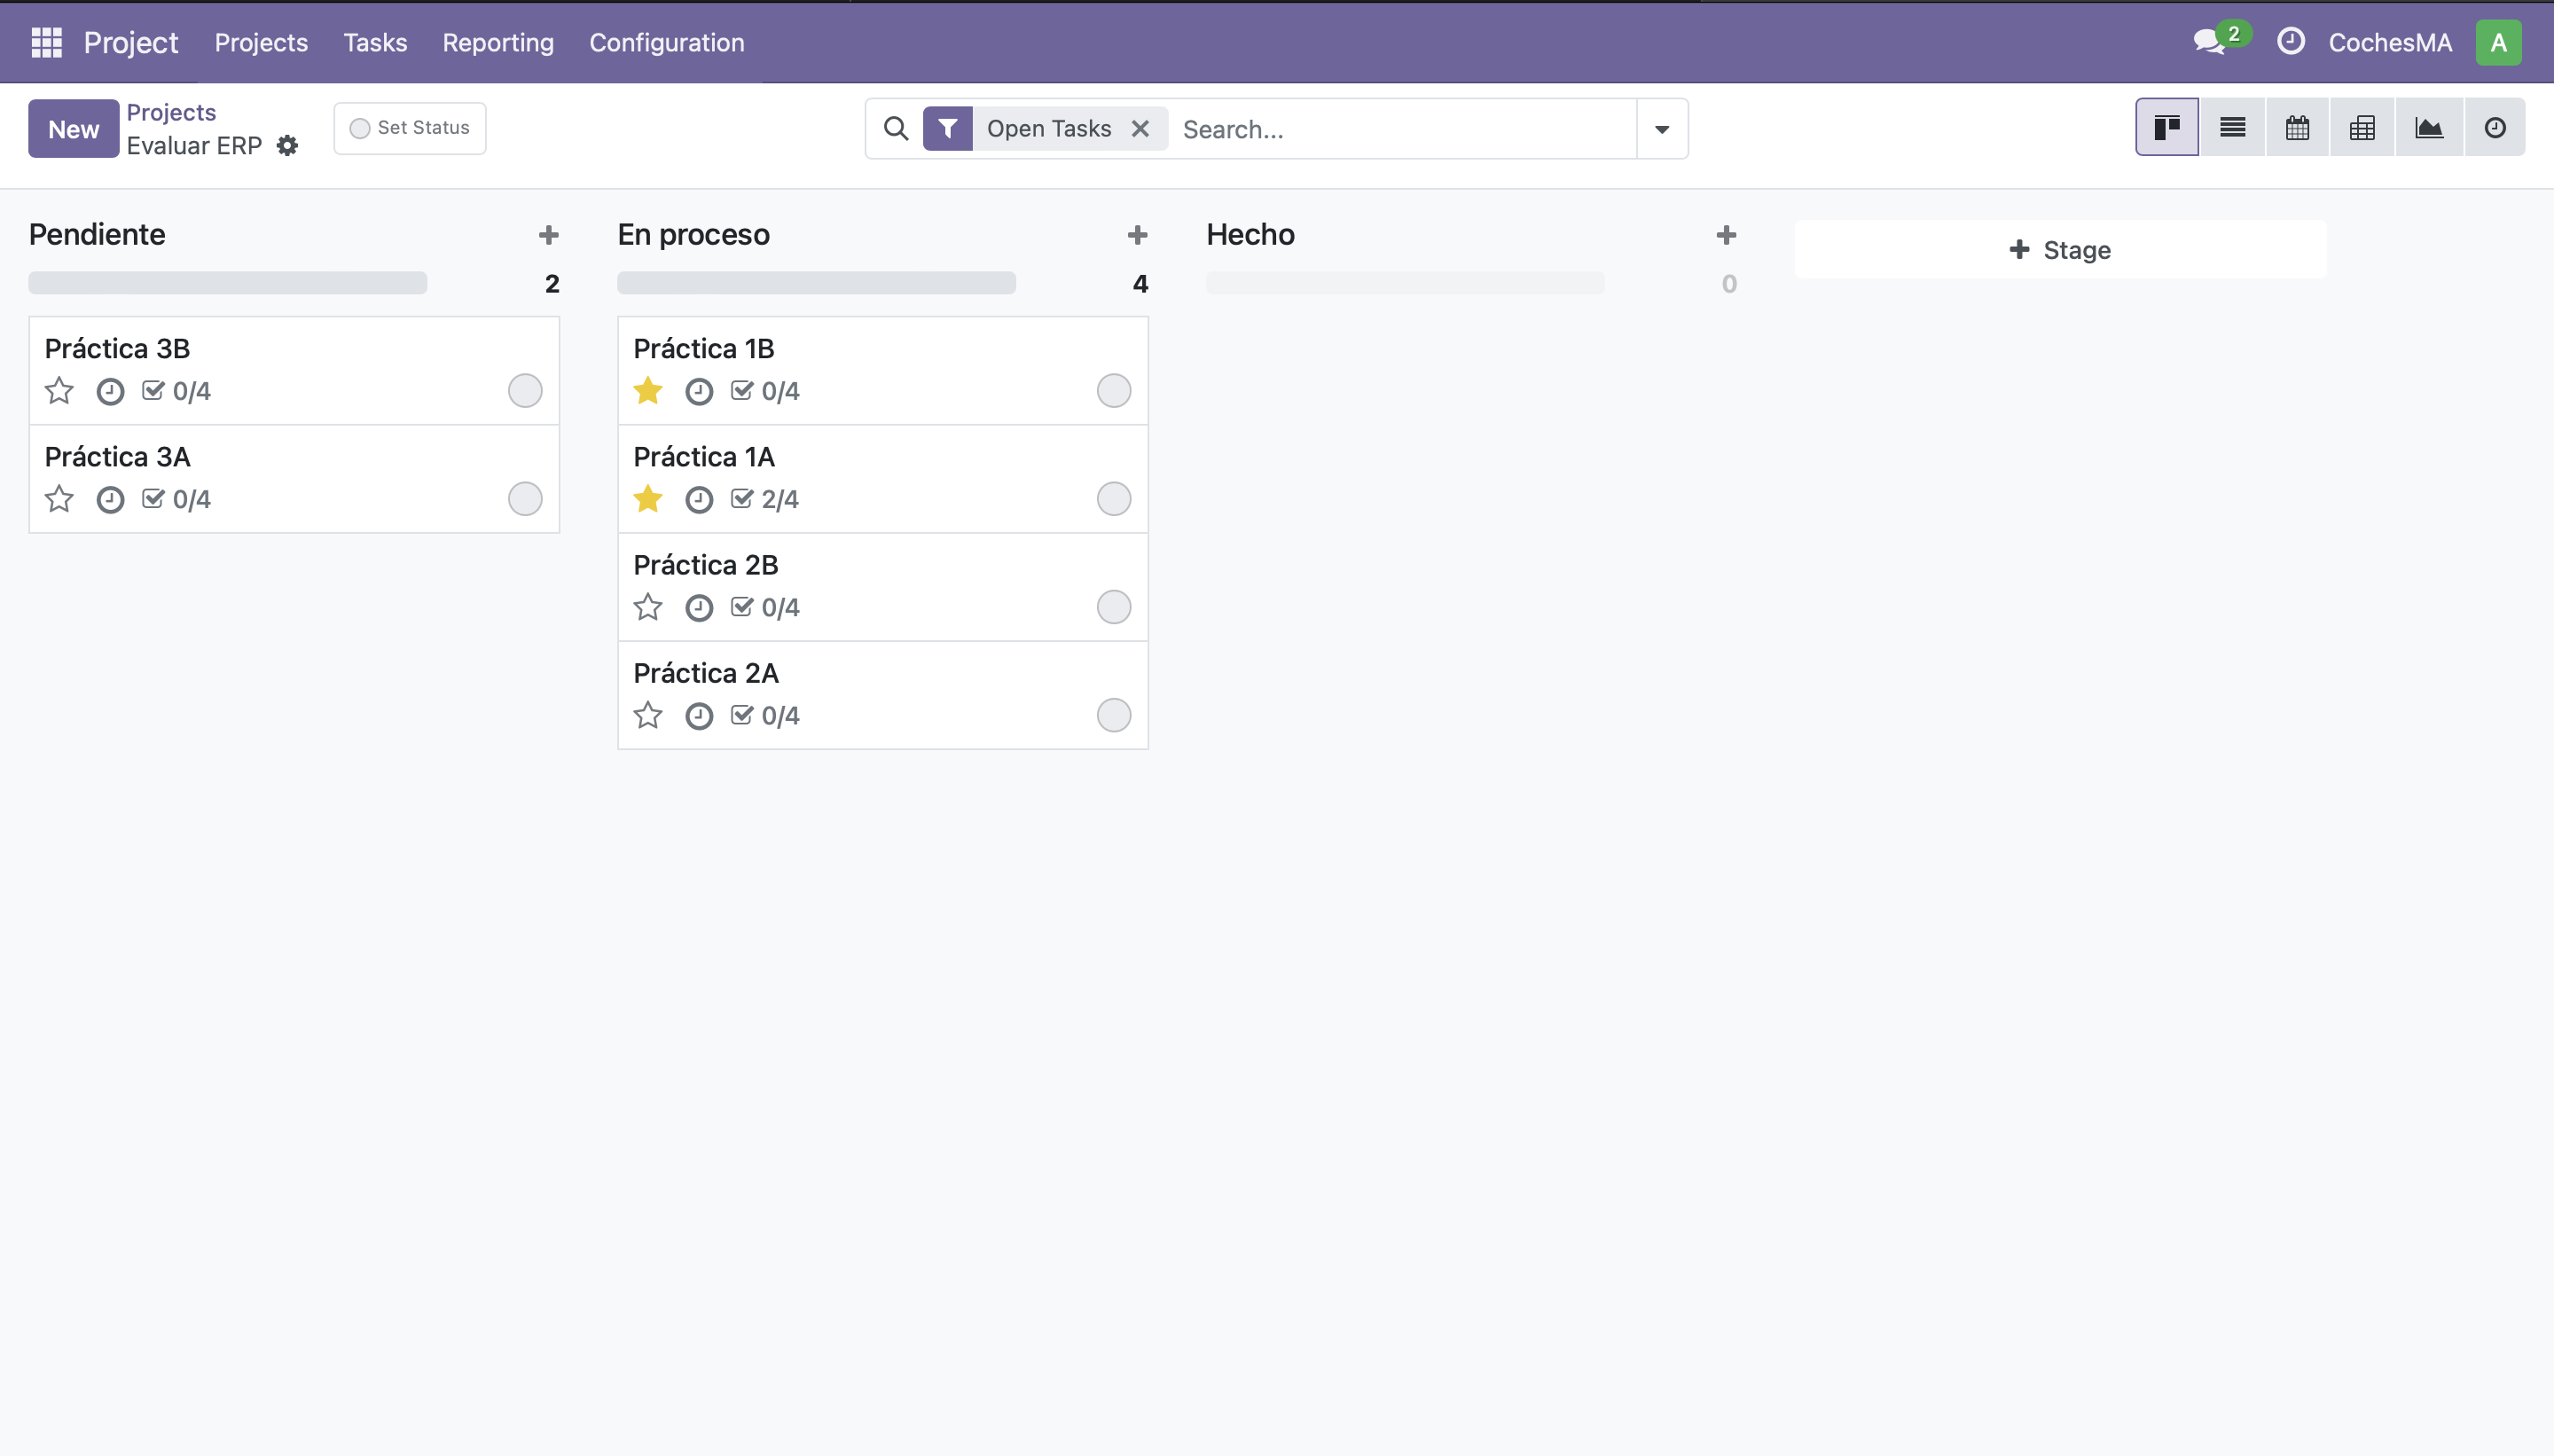
\includegraphics[width=10cm]{completedSubtaskProject.png}
    \caption{Sub-tareas vista general.}
    \label{fig:openProyectos}
\end{figure}
\subsection{Bloqueo de tareas}
\paragraph{}
Por último, se puede bloquear una tarea hasta que otra tarea se haya completado. Para ello es necesario configurar nuestro projecto. Abrimos los ajustes del projecto y activamos la opción \textit{Task Dependencies}. Tras cambiar la configuración pulsa en la tarea que quieres bloquear y selecciona la opción \textit{Block by} y selecciona la tarea que bloquea. En nuestro caso hemos bloqueado la tarea \textit{Práctica 1B} hasta que se complete la tarea \textit{Práctica 1A}. Para saber si hemos bloqueado una tarea, se mostrará un relon de arena en la tarea que está bloqueada.
\begin{figure}[h]
    \centering
    \includegraphics[width=10cm]{settingsProject.png}
    \caption{Ajustes del proyecto .}
    \label{fig:openProyectos}
\end{figure}
\begin{figure}[h]
    \centering
    \includegraphics[width=10cm]{blockTaskProject.png}
    \caption{Bloque de tarea.}
    \label{fig:openProyectos}
\end{figure}
\begin{figure}[h]
    \centering
    \includegraphics[width=10cm]{viewBlockProject.png}
    \caption{Visualizar bloqueo de tarea.}
    \label{fig:openProyectos}
\end{figure}






\end{document} 
